\documentclass[11pt,oneside]{book}
\usepackage{fontspec}
\setmainfont{Noto Serif}
\setsansfont{Noto Sans}
\setmonofont{Noto Sans Mono}
\newfontfamily\proseunicodefont{DejaVu Serif}
\usepackage[margin=1in]{geometry}
\usepackage{microtype}
\usepackage{amsmath,amssymb,amsthm,mathtools,bm}
\usepackage{graphicx}
\usepackage{adjustbox}
\usepackage{xcolor}
\usepackage{booktabs}
\usepackage{array}
\usepackage{longtable}
\usepackage{enumitem}
\usepackage{float}
\usepackage{caption}
\usepackage{hyperref}
\usepackage{fancyhdr}
\usepackage{tikz}
\usetikzlibrary{arrows.meta,positioning,calc,decorations.pathmorphing}

\hypersetup{
  colorlinks=true,
  linkcolor=blue!50!black,
  urlcolor=blue!50!black,
  citecolor=blue!50!black
}

\setlength{\parskip}{0.5em}
\setlength{\parindent}{0pt}
\setlist[itemize]{topsep=0.25em,itemsep=0.2em}
\setlist[enumerate]{topsep=0.25em,itemsep=0.2em}
\setlength{\headheight}{40pt}
\numberwithin{equation}{chapter}

\newtheorem{theorem}{Định lý}[chapter]
\newtheorem{proposition}[theorem]{Mệnh đề}
\newtheorem{lemma}[theorem]{Bổ đề}
\newtheorem{corollary}[theorem]{Hệ quả}
\theoremstyle{definition}
\newtheorem{definition}[theorem]{Định nghĩa}
\newtheorem{example}[theorem]{Ví dụ}
\theoremstyle{remark}
\newtheorem{remark}[theorem]{Nhận xét}

\providecommand{\ket}[1]{\left\lvert#1\right\rangle}
\providecommand{\bra}[1]{\left\langle#1\right\rvert}
\providecommand{\braket}[2]{\left\langle#1\,\middle|\,#2\right\rangle}
\providecommand{\expect}[1]{\left\langle#1\right\rangle}
\newcommand{\lectureoverview}[1]{\paragraph{Tổng quan.} #1}

\makeatletter
\newcommand{\course@headerfont}{\normalfont\small\itshape}
\newcommand{\course@pagefont}{\normalfont\small}
\newcommand{\course@headerraise}{14pt}
\newlength{\course@headerboxheight}
\setlength{\course@headerboxheight}{\dimexpr\headheight-\course@headerraise-9pt\relax}
\newcommand{\course@leftheadbox}[1]{%
  \raisebox{\course@headerraise}{%
    \parbox[t][\course@headerboxheight][t]{0.82\textwidth}{%
      \raggedright\course@headerfont\strut\MakeUppercase{#1}\strut%
    }%
  }%
}
\newcommand{\course@rightheadbox}[1]{%
  \raisebox{\course@headerraise}{%
    \parbox[t][\course@headerboxheight][t]{0.82\textwidth}{%
      \raggedleft\course@headerfont\strut\MakeUppercase{#1}\strut%
    }%
  }%
}
\renewcommand{\chaptermark}[1]{\markboth{\MakeUppercase{\chaptername\ \thechapter.\ #1}}{}}
\renewcommand{\sectionmark}[1]{\markright{\MakeUppercase{\thesection\hspace{0.4em}#1}}}
\fancyhf{}
\fancyhead[L]{\course@leftheadbox{\leftmark}}
\fancyhead[R]{\course@pagefont\thepage}
\renewcommand{\headrulewidth}{0.5pt}
\pagestyle{fancy}
\fancypagestyle{plain}{%
  \fancyhf{}
  \fancyhead[L]{\course@leftheadbox{\leftmark}}
  \fancyhead[R]{\course@pagefont\thepage}
  \renewcommand{\headrulewidth}{0.5pt}
}
\makeatother

% Video2Book editorial provenance macros
\newenvironment{classroomqa}{%
  \par\medskip\noindent\begin{minipage}{\linewidth}\small\hrule\medskip
}{%
  \medskip\hrule\end{minipage}\par\medskip
}
\newcommand{\audiencequestion}[1]{\noindent\textbf{Câu hỏi từ người nghe.} #1\par\smallskip}
\newcommand{\lecturerresponse}[1]{\noindent\textbf{Trả lời.} #1\par}
\newcommand{\lecturetimestamp}[1]{\footnote{Mốc thời gian bài giảng: #1.}}
\newcommand{\lectureframe}[1]{\par\smallskip{\centering\footnotesize\itshape Khung hình bài giảng: #1.\par}}
\newcommand{\editorialnote}[1]{\footnote{Chú giải biên tập: #1}}

\usepackage{polyglossia}
\setdefaultlanguage{vietnamese}
\usepackage{sectsty}
\renewcommand{\contentsname}{Mục lục}
\renewcommand{\chaptername}{Chương}
\renewcommand{\figurename}{Hình}
\renewcommand{\tablename}{Bảng}
\renewcommand{\proofname}{Chứng minh}
\renewcommand{\bibname}{Tài liệu tham khảo}
\sectionfont{\raggedright}
\subsectionfont{\raggedright}
\makeatletter
\renewcommand{\@pnumwidth}{2.2em}
\renewcommand{\@tocrmarg}{3.2em}
\makeatother
\usepackage{tocloft}
\renewcommand{\cftchapfont}{\small\bfseries}
\renewcommand{\cftchappagefont}{\small\bfseries}
\renewcommand{\cftsecfont}{\small}
\renewcommand{\cftsecpagefont}{\small}
\setlength{\cftsecnumwidth}{3em}
\renewcommand{\cftsubsecfont}{\small}
\renewcommand{\cftsubsecpagefont}{\small}
\setlength{\cftsubsecindent}{4.5em}
\setlength{\cftsubsecnumwidth}{4em}
\emergencystretch=6em
\pdfstringdefDisableCommands{\def\proseunicodefont{}}

\geometry{paperwidth=177.6mm,paperheight=252mm,left=16mm,right=16mm,
 top=18mm,bottom=18mm,includeheadfoot,headheight=28pt,headsep=7mm,footskip=9mm}
\usepackage{scrextend}
\changefontsizes[17pt]{12pt}
\raggedbottom
\renewenvironment{classroomqa}{\par\medskip\begingroup}{\par\endgroup\medskip}
\fancyhf{}
\setlength{\headwidth}{\textwidth}
\fancyhead[L]{\parbox{\textwidth}{\raggedright\fontsize{9}{11}\selectfont\nouppercase{\leftmark}}}
\fancyfoot[C]{\small\thepage}
\renewcommand{\headrulewidth}{0.3pt}
\fancypagestyle{plain}{\fancyhf{}\fancyfoot[C]{\small\thepage}\renewcommand{\headrulewidth}{0pt}}

\graphicspath{{../../../generated_course_notes/supplementary/advanced_quantum_mechanics/2013_fall/figures/}{../../../generated_course_notes/supplementary/advanced_quantum_mechanics/2013_fall/assets/}}
\begin{document}
\frontmatter
\hypersetup{pageanchor=false}
\begin{titlepage}
\hyphenpenalty=10000\exhyphenpenalty=10000
\thispagestyle{empty}
\begin{tikzpicture}[remember picture,overlay]
  \node[anchor=center,inner sep=0] at (current page.center) {%
    \includegraphics[height=\paperheight,keepaspectratio]{../../../generated_course_notes/supplementary/advanced_quantum_mechanics/2013_fall/assets/cover-art.png}%
  };
  \node[
    anchor=north west,
    align=left,
    text width=0.78\paperwidth,
    fill=white,
    fill opacity=0.9,
    rounded corners=8pt,
    inner xsep=10pt,
    inner ysep=8pt
  ] at ([xshift=0.08\paperwidth,yshift=-0.06\paperheight]current page.north west) {%
    {\fontsize{30}{33}\selectfont\bfseries\color{black!88} Cơ học lượng tử nâng cao\\[0.85em]}
    {\large\color{black!72} Bản tiếng Việt / mùa thu 2013}
  };
  \node[
    anchor=south west,
    align=left,
    text width=0.68\paperwidth,
    fill=white,
    fill opacity=0.82,
    text opacity=1,
    rounded corners=6pt,
    inner sep=12pt
  ] at ([xshift=0.08\paperwidth,yshift=0.08\paperheight]current page.south west) {%
    {\normalsize\color{black!78} Bài giảng gốc: Leonard Susskind\\[0.35em]}
    {\small\color{black!72} Ấn bản đồng hành: \href{https://lazying.art}{LazyingArt LLC} / \href{https://github.com/lachlanchen/Video2Book}{Video2Book}}
  };
\end{tikzpicture}
\mbox{}
\end{titlepage}
\hypersetup{pageanchor=true}

\clearpage
\chapter*{Về những ghi chú này}
Những ghi chú đồng hành được biên tập độc lập này dựa theo các bài giảng của Leonard Susskind. Chúng được phục dựng từ bản chép lời do máy tạo, phụ đề và một số khung hình được chọn lọc từ bảng, sau đó đối chiếu với các tư liệu nguồn hiện có. Đây không phải là bản thảo gốc của Giáo sư Susskind, và ông cũng chưa xem xét hay chứng thực những ghi chú này.

Ấn bản được \href{https://lazying.art}{LazyingArt LLC} biên soạn bằng quy trình mã nguồn mở \href{https://github.com/lachlanchen/Video2Book}{Video2Book}. Bản chép lời do máy tạo được cung cấp riêng và có thể có lỗi nhận dạng. Những phần làm rõ về biên tập và những chỗ phục dựng đáng kể được ghi rõ trong chú thích.
\clearpage
\tableofcontents
\mainmatter
\chapter{Vectơ trạng thái, sự tiến hóa unita và đối xứng tịnh tiến}
\providecommand{\ket}[1]{\left\lvert#1\right\rangle}
\providecommand{\bra}[1]{\left\langle#1\right\rvert}

Sau khoảng nghỉ hai quý, việc ôn nhanh cơ học lượng tử sẽ rất hữu ích. Tuy nhiên, không thể dành trọn cả quý cho việc ôn tập. Chủ đề tiếp theo là ứng dụng cơ học lượng tử vào những bài toán mà ban đầu lý thuyết này được phát triển để giải quyết: nguyên tử, electron và các hạt liên quan, cùng photon.

Trước hết là nguyên tử. Làm sao có thể xét nguyên tử trước electron, khi electron là thành phần của nguyên tử? Ban đầu, chỉ cần biết vừa đủ về cơ học của electron để viết các phương trình cơ bản của nguyên tử hydro. Sau đó có thể nghiên cứu chi tiết hơn về các hạt giống electron. Trong suốt những ứng dụng này, đối xứng sẽ là công cụ thường xuyên được sử dụng: cách các đối xứng được biểu diễn trong cơ học lượng tử và những hệ quả của chúng đối với một hệ.

\section{Trạng thái, đại lượng quan sát được và tính trực giao}

Trong cơ học cổ điển, trạng thái được biểu diễn bằng một điểm trong không gian pha. Trong cơ học lượng tử, trạng thái được biểu diễn bằng một vectơ trong một không gian vectơ phức. Đây là vectơ trừu tượng, không phải mũi tên trong không gian ba chiều thông thường. Có thể cộng các vectơ trạng thái và nhân chúng với các số phức; không gian chứa chúng không nhất thiết phải có số chiều hữu hạn cụ thể nào.

Ký hiệu Dirac viết vectơ trạng thái dưới dạng ket,
\begin{equation}
\ket{\psi},
\end{equation}
và gắn với nó một bra,
\begin{equation}
\bra{\psi}.
\end{equation}
Bra và ket liên hệ với nhau qua phép liên hợp Hermite. Ghép một bra với một ket ta được tích vô hướng,
\begin{equation}
\langle\phi|\psi\rangle,
\end{equation}
vốn thường là một số phức.

Đại lượng quan sát được là đại lượng có thể đo: vị trí, động lượng, năng lượng hay bất kỳ đại lượng đo được nào khác. Trong cơ học lượng tử, một đại lượng quan sát được được biểu diễn bằng toán tử tuyến tính Hermite \(A\),
\begin{equation}
A^\dagger=A.
\end{equation}
Tính Hermite là dạng tương tự của tính thực đối với toán tử. Cụ thể, các trị riêng của một toán tử Hermite đều là số thực.

Vectơ riêng của \(A\) thỏa mãn
\begin{equation}
A\ket{\alpha}=\alpha\ket{\alpha}.
\end{equation}
Các trị riêng có thể có chính là những kết quả có thể thu được khi đo \(A\). Chẳng hạn, nếu một đại lượng quan sát được chỉ có thể cho kết quả \(1\), \(3\) hoặc \(7\), thì những số này là các trị riêng của nó. Các vectơ riêng là những trạng thái trong đó kết quả được xác định rõ, chứ không mang tính thống kê. Ở trạng thái \(\ket{\alpha}\), phép đo \(A\) chắc chắn cho kết quả \(\alpha\).

Tích vô hướng biểu thị một quan hệ logic quan trọng giữa các trạng thái. Giả sử có một phép đo có thể phân biệt chắc chắn \(\ket{\phi}\) với \(\ket{\psi}\). Khi đó hai trạng thái trực giao với nhau:
\begin{equation}
\langle\phi|\psi\rangle=0.
\end{equation}
Tính trực giao nghĩa là có thể phân biệt các trạng thái về mặt vật lý mà không có sự nhập nhằng. Với một trạng thái đã chuẩn hóa,
\begin{equation}
\langle\psi|\psi\rangle=1.
\end{equation}

\section{Hạt trong biểu diễn vị trí}

Trước hết, xét một hạt chuyển động trên một đường thẳng. Vị trí \(x\) của hạt là một đại lượng quan sát được. Với mỗi vị trí có thể có \(x_0\), tồn tại một trạng thái \(\ket{x_0}\) mà trong đó phép đo vị trí chắc chắn cho kết quả \(x_0\).

Các trạng thái ứng với những vị trí khác nhau có thể phân biệt được, nên chúng trực giao:
\begin{equation}
x\neq x'
\quad\Longrightarrow\quad
\langle x'|x\rangle=0.
\end{equation}
Với một trạng thái bất kỳ \(\ket{\psi}\), độ chồng lấp của nó với trạng thái vị trí xác định hàm sóng:
\begin{equation}
\psi(x)=\langle x|\psi\rangle.
\end{equation}
Đây là biểu diễn vị trí của vectơ trạng thái.

Bản thân hàm sóng không phải là xác suất. Hàm sóng có thể dương, âm, ảo hoặc hoàn toàn phức. Mật độ xác suất vị trí là
\begin{equation}
P(x)=\psi^*(x)\psi(x)=|\psi(x)|^2.
\end{equation}
Tích này không âm, đúng như yêu cầu đối với một mật độ xác suất. Với hàm sóng đã chuẩn hóa,
\begin{equation}
\int_{-\infty}^{\infty}dx\,|\psi(x)|^2=1.
\end{equation}

Trong biểu diễn vị trí, toán tử vị trí tác dụng bằng phép nhân:
\begin{equation}
(\hat x\psi)(x)=x\psi(x).
\end{equation}
Các hàm riêng của nó là những hàm lý tưởng tập trung tại một điểm. Về mặt hình thức, chúng được mô tả bằng các hàm delta Dirac: những đỉnh rất hẹp có tâm tại trị riêng vị trí. Không cần đến định nghĩa phân phối chính xác của chúng trong phần ôn tập này.

Trong ba chiều, vị trí có ba thành phần \(x\), \(y\) và \(z\); trạng thái vị trí biểu diễn một điểm trong không gian ba chiều. Hai trạng thái như vậy trực giao nếu các điểm tương ứng khác nhau ít nhất ở một tọa độ. Thông thường, ta vẫn dùng ký hiệu một chiều và ngầm hiểu phần mở rộng tương ứng sang ba chiều.

\section{Động lượng và các trạng thái có động lượng xác định}

Mỗi thành phần vị trí có một thành phần động lượng tương ứng. Trong biểu diễn vị trí, toán tử động lượng dọc theo trục \(x\) là
\begin{equation}
\hat p_x=-i\hbar\frac{d}{dx}.
\end{equation}
Như vậy, một toán tử Hermite trừu tượng cũng có thể được hình dung cụ thể như một phép toán tác động lên các hàm sóng.

Trạng thái có động lượng xác định \(p_0\) thỏa mãn phương trình trị riêng
\begin{equation}
\hat p_x\psi_{p_0}(x)=p_0\psi_{p_0}(x).
\end{equation}
Thay dạng vi phân của \(\hat p_x\) vào ta được
\begin{equation}
-i\hbar\frac{d\psi_{p_0}(x)}{dx}
=p_0\psi_{p_0}(x).
\end{equation}
Đạo hàm của hàm sóng tỉ lệ với chính hàm sóng, nên nghiệm có dạng hàm mũ:
\begin{equation}
\psi_{p_0}(x)\propto
\exp\left(\frac{ip_0x}{\hbar}\right).
\end{equation}

\begin{classroomqa}
\lecturetimestamp{00:24:26}
\audiencequestion{Phương trình vi phân này có đúng với mọi hàm sóng không?}
\lecturerresponse{Không. Đây là phương trình trị riêng cho trạng thái có động lượng xác định. Phần lớn các hàm sóng không thỏa mãn phương trình này; nó chọn ra các hàm riêng động lượng.}
\end{classroomqa}

Sự khác biệt giữa trạng thái riêng vị trí và trạng thái riêng động lượng rất rõ rệt. Hàm riêng vị trí tập trung tại một điểm. Hàm riêng động lượng có
\begin{equation}
\left|\exp\left(\frac{ip_0x}{\hbar}\right)\right|^2=1.
\end{equation}
Do đó, môđun của nó không đổi trên toàn bộ đường thẳng. Theo nghĩa lý tưởng hóa này, động lượng xác định đồng nghĩa với độ bất định hoàn toàn về vị trí; tương tự, vị trí xác định cũng đồng nghĩa với độ bất định hoàn toàn về động lượng. Đây là trường hợp cực hạn của hệ thức bất định vị trí--động lượng.

\begin{classroomqa}
\lecturetimestamp{00:26:36}
\audiencequestion{Nếu biết động lượng là \(p_0\), tại sao vẫn có phân bố xác suất?}
\lecturerresponse{Đại lượng được trình bày ở đây liên quan đến phép đo vị trí, chứ không phải một phép đo động lượng khác. Động lượng và vị trí là hai đại lượng quan sát được khác nhau. Với trạng thái riêng động lượng lý tưởng hóa, biên độ vị trí có môđun không đổi trên toàn bộ đường thẳng. Biên độ động lượng thuộc về biểu diễn động lượng và liên hệ với hàm sóng vị trí qua phép biến đổi Fourier.}
\end{classroomqa}

\begin{classroomqa}
\lecturetimestamp{00:28:02}
\audiencequestion{Xác suất vị trí có dạng thế nào khi hàm sóng là hàm delta Dirac?}
\lecturerresponse{Nó tập trung tại vị trí đã chỉ định. Đỉnh lý tưởng hóa biểu thị vị trí được xác định chắc chắn.}
\end{classroomqa}

\editorialnote{Các trạng thái riêng vị trí và động lượng chính xác là những trạng thái tổng quát hóa. Hàm delta Dirac và sóng phẳng không phải là các hàm sóng thông thường, bình phương khả tích và được chuẩn hóa trên toàn đường thẳng; bình phương theo nghĩa thông thường của một hàm delta cũng không phải là một phân phối thông thường. Những phát biểu trên nói về tính định xứ lý tưởng hóa và môđun không đổi của chúng.}

Về mặt hình thức, có thể xem hàm sóng như một vectơ có một thành phần ứng với mỗi giá trị của \(x\). Tuy nhiên, không giống một vectơ cột hữu hạn thông thường, nó có vô hạn liên tục các thành phần.

\begin{classroomqa}
\lecturetimestamp{00:28:53}
\audiencequestion{Vectơ trạng thái có được biểu diễn bằng vectơ cột không?}
\lecturerresponse{Có thể biểu diễn như vậy, nhưng viết một hàm sóng vị trí dưới dạng vectơ cột thông thường khá bất tiện vì \(x\) nhận liên tục nhiều giá trị. Có thể hình dung nó về mặt hình thức như một vectơ cột liên tục, còn bra tương ứng là một vectơ hàng liên tục.}
\end{classroomqa}

\section{Sự tiến hóa theo thời gian và tính unita}

Trạng thái thay đổi theo thời gian như thế nào? Sự tiến hóa theo thời gian là một phép biến đổi trên không gian trạng thái. Gọi \(U(t)\) là toán tử biểu thị sự tiến hóa trong khoảng thời gian đã trôi qua \(t\). Khi đó,
\begin{equation}
U(t)\ket{\psi(t_1)}=\ket{\psi(t_1+t)}.
\end{equation}
Đặc biệt,
\begin{equation}
\ket{\psi(t)}=U(t)\ket{\psi(0)},
\qquad
U(0)=\mathbf 1.
\end{equation}

Điều kiện đối với \(U(t)\) bắt nguồn từ định luật bảo toàn thông tin. Nếu hai trạng thái ban đầu có thể phân biệt được, sự tiến hóa theo thời gian không được xóa nhòa sự khác biệt đó. Các trạng thái trực giao phải tiếp tục trực giao. Tổng quát hơn, tích vô hướng giữa hai trạng thái bất kỳ được bảo toàn:
\begin{equation}
\langle U(t)\phi|U(t)\psi\rangle
=\langle\phi|\psi\rangle.
\end{equation}
Vì
\begin{equation}
\langle U(t)\phi|U(t)\psi\rangle
=\langle\phi|U^\dagger(t)U(t)|\psi\rangle,
\end{equation}
việc bảo toàn mọi tích vô hướng đòi hỏi
\begin{equation}
U^\dagger(t)U(t)=\mathbf 1.
\end{equation}
Toán tử thỏa mãn phương trình này được gọi là toán tử unita.

\begin{classroomqa}
\lecturetimestamp{00:36:36}
\audiencequestion{Bảo toàn mọi tích vô hướng có phải là một điều kiện mạnh hơn chỉ bảo toàn tính trực giao không?}
\lecturerresponse{Đối với các phép biến đổi tuyến tính của trạng thái đang xét, bảo toàn tính trực giao dẫn đến bảo toàn tích vô hướng. Phép quay thông thường là một phép tương tự quen thuộc: nó bảo toàn tính trực giao và tích vô hướng.}
\end{classroomqa}

\editorialnote{Nói chính xác, chỉ bảo toàn tính trực giao vẫn cho phép một hệ số co giãn chung khác không. Việc bảo toàn chuẩn hóa, vốn đã là yêu cầu đối với sự tiến hóa vật lý theo thời gian, loại bỏ khả năng đó và dẫn đến bảo toàn tích vô hướng.}

Không nên nhầm toán tử unita với các đại lượng quan sát được Hermite. Vị trí và động lượng là các toán tử Hermite, nhưng nhìn chung chúng không phải là toán tử unita. Các trị riêng của một toán tử unita là các pha, tức những số có dạng \(e^{i\theta}\) và nằm trên đường tròn đơn vị.

\begin{classroomqa}
\lecturetimestamp{00:38:12}
\audiencequestion{Ví dụ nào về một phép biến đổi không unita?}
\lecturerresponse{Các toán tử vị trí và động lượng là những ví dụ: chúng là các đại lượng quan sát được Hermite nhưng không unita. Toán tử unita có các trị riêng với môđun bằng đơn vị, nên các trị riêng của nó là các pha.}
\end{classroomqa}

\section{Hamiltonian và phương trình Schr\"odinger}

Giả sử sự tiến hóa theo thời gian là liên tục. Vì vậy, trong một khoảng thời gian rất ngắn \(\epsilon\), toán tử tiến hóa phải gần với toán tử đồng nhất:
\begin{equation}
U(\epsilon)=\mathbf 1+\epsilon G+\mathcal O(\epsilon^2).
\end{equation}
Dùng tính unita,
\begin{align}
U^\dagger(\epsilon)U(\epsilon)
&=
\left(\mathbf 1+\epsilon G^\dagger\right)
\left(\mathbf 1+\epsilon G\right)
+\mathcal O(\epsilon^2)
\\
&=
\mathbf 1+\epsilon(G^\dagger+G)
+\mathcal O(\epsilon^2).
\end{align}
Ở bậc nhất,
\begin{equation}
G^\dagger=-G.
\end{equation}
Do đó \(G\) là phản Hermite. Có thể viết nó dưới dạng
\begin{equation}
G=-\frac{i}{\hbar}H,
\end{equation}
trong đó \(H\) là toán tử Hermite:
\begin{equation}
H^\dagger=H.
\end{equation}
Vì vậy, toán tử tiến hóa trong thời gian vi phân là
\begin{equation}
U(\epsilon)
=
\mathbf 1-\frac{i\epsilon}{\hbar}H
+\mathcal O(\epsilon^2).
\end{equation}
Toán tử Hermite \(H\) được gọi là Hamiltonian.

\begin{classroomqa}
\lecturetimestamp{00:45:48}
\audiencequestion{Vì sao có thể bỏ qua số hạng \(\epsilon^2\)?}
\lecturerresponse{Phép tính được thực hiện nhất quán đến bậc nhất theo \(\epsilon\). Nếu tính đến bậc hai thì phải giữ tất cả các số hạng bậc hai, kể cả số hạng tỉ lệ với \(-\epsilon^2H^2/(2\hbar^2)\). Phép gần đúng nằm ở biểu thức đã lược bỏ các số hạng của \(U(\epsilon)\), chứ không nằm trong tính Hermite của \(H\).}
\end{classroomqa}

Có thể ghép một khoảng thời gian hữu hạn từ nhiều khoảng nhỏ. Chia \(t\) thành \(N\) bước, mỗi bước dài \(t/N\). Lặp lại phép biến đổi vi phân ta được
\begin{equation}
U(t)
=
\lim_{N\to\infty}
\left(
\mathbf 1-\frac{itH}{N\hbar}
\right)^N
=
\exp\left(-\frac{iHt}{\hbar}\right).
\end{equation}
Hàm mũ là dạng hữu hạn của phép biến đổi vi phân.

Giờ hãy cho trạng thái tiến hóa từ \(t\) đến \(t+\epsilon\):
\begin{align}
\ket{\psi(t+\epsilon)}
&=
U(\epsilon)\ket{\psi(t)}
\\
&=
\left(
\mathbf 1-\frac{i\epsilon}{\hbar}H
\right)\ket{\psi(t)}
+\mathcal O(\epsilon^2).
\end{align}
Lấy hiệu với \(\ket{\psi(t)}\), chia cho \(\epsilon\) rồi lấy giới hạn, ta được
\begin{equation}
\frac{d}{dt}\ket{\psi(t)}
=
-\frac{i}{\hbar}H\ket{\psi(t)}.
\end{equation}
Tương đương,
\begin{equation}
i\hbar\frac{d}{dt}\ket{\psi(t)}
=
H\ket{\psi(t)}.
\end{equation}
Đây là phương trình Schr\"odinger phụ thuộc thời gian. Trong biểu diễn vị trí, phương trình trở thành
\begin{equation}
i\hbar\frac{\partial}{\partial t}\psi(x,t)
=
H\psi(x,t),
\end{equation}
trong đó \(H\) tác dụng như một toán tử lên hàm sóng.

Phương trình Schr\"odinger không phụ thuộc thời gian là phương trình trị riêng của Hamiltonian:
\begin{equation}
H\ket{E}=E\ket{E}.
\end{equation}
Các trị riêng \(E\) là những năng lượng có thể đo được, hay các mức năng lượng. Vì vậy, cùng một Hamiltonian xác định cả những năng lượng được phép lẫn sự tiến hóa của trạng thái.

Nếu trạng thái ban đầu là một trạng thái riêng năng lượng, sự tiến hóa của nó là
\begin{equation}
\ket{E;t}
=
\exp\left(-\frac{iEt}{\hbar}\right)\ket{E}.
\end{equation}
Nó vẫn là cùng một vectơ riêng năng lượng và chỉ nhận thêm một pha.\footnote{Dấu trừ được xác định từ phép suy ra \(U(t)=\exp(-iHt/\hbar)\) ở trên. Cách đọc thành lời của pha ở phần sau có dấu ngược lại và không nhất quán với phép suy ra đó.}

\begin{classroomqa}
\lecturetimestamp{01:01:05}
\audiencequestion{Vectơ riêng năng lượng tiến hóa như thế nào theo phương trình Schr\"odinger phụ thuộc thời gian?}
\lecturerresponse{Giữ nguyên ket. Vì \(H\ket{E}=E\ket{E}\), sự tiến hóa theo thời gian nhân vectơ riêng năng lượng với một pha được xác định bởi năng lượng của nó: \(\exp(-iEt/\hbar)\).}
\end{classroomqa}

\section{Thế nào là một đối xứng?}

Sự tiến hóa theo thời gian là một phép biến đổi unita trên không gian trạng thái. Các phép biến đổi đối xứng là một lớp quan trọng khác.

Đối xứng quay giữ vai trò trung tâm trong vật lý nguyên tử. Trong nguyên tử hydro, electron chuyển động trong thế Coulomb tâm. Phép quay hệ tọa độ không làm thay đổi các phương trình; còn khi quay nguyên tử trên thực tế, nguyên tử vẫn tuân theo cùng các phương trình ấy. Trạng thái có thể thay đổi khi quay, nhưng định luật động lực học thì không.

Tịnh tiến là một ví dụ khác. Một hệ cô lập trong không gian trống phải có cách ứng xử như nhau sau khi mọi bộ phận của nó cùng được dịch đi một khoảng như nhau. Điều kiện giới hạn này rất quan trọng. Nếu có một lò nung và chỉ dịch chuyển hệ lại gần lò, hệ có thể ứng xử khác đi; lò nung phá vỡ đối xứng tịnh tiến đó. Nếu dịch chuyển cả hệ lẫn lò nung cùng nhau, quan hệ ban đầu giữa chúng được khôi phục.

Không phải phép biến đổi nào cũng là đối xứng. Nén tinh thể muối mỏ theo hệ số hai thường làm thay đổi cách tinh thể ứng xử. Ép là một phép biến đổi xác định rõ, nhưng nhìn chung không phải là đối xứng.

Vì vậy, đối xứng là một phép biến đổi trên các trạng thái bảo toàn dạng thức của động lực học. Ký hiệu phép biến đổi đó là \(V\). Nó phải bảo toàn khả năng phân biệt: hai trạng thái trực giao phải vẫn trực giao sau phép biến đổi. Do đó,
\begin{equation}
V^\dagger V=\mathbf 1,
\end{equation}
nên \(V\) là unita.

\section{Đối xứng giao hoán với sự tiến hóa theo thời gian}

Giả sử trạng thái ban đầu \(\ket{\psi_1}\) tiến hóa thành \(\ket{\psi_2}\):
\begin{equation}
\ket{\psi_2}=U(t)\ket{\psi_1}.
\end{equation}
Áp dụng phép đối xứng được đề xuất \(V\) lên cả hai trạng thái:
\begin{equation}
\ket{\psi_1'}=V\ket{\psi_1},
\qquad
\ket{\psi_2'}=V\ket{\psi_2}.
\end{equation}
Nếu \(V\) là đối xứng của động lực học, trạng thái ban đầu sau biến đổi phải tiến hóa thành trạng thái cuối sau biến đổi:
\begin{equation}
\ket{\psi_2'}=U(t)\ket{\psi_1'}.
\end{equation}
Thay các định nghĩa vào, ta được
\begin{equation}
VU(t)\ket{\psi_1}
=
U(t)V\ket{\psi_1}.
\end{equation}
Điều này phải đúng với mọi trạng thái ban đầu. Do đó,
\begin{equation}
VU(t)=U(t)V.
\end{equation}

Hai lộ trình tương đương có thể được biểu diễn bằng một sơ đồ giao hoán.\footnote{Sơ đồ tái hiện lập luận hai lộ trình được triển khai từ 01:10:30 đến 01:16:34.}
\begin{figure}
\centering
\begin{tikzpicture}[>=Stealth]
\node (a) at (0,0) {$\ket{\psi_1}$};
\node (b) at (4.2,0) {$\ket{\psi_2}=U(t)\ket{\psi_1}$};
\node (c) at (0,-2.0) {$V\ket{\psi_1}$};
\node (d) at (4.2,-2.0) {$V\ket{\psi_2}=U(t)V\ket{\psi_1}$};

\draw[->] (a) -- node[above] {$U(t)$} (b);
\draw[->] (c) -- node[below] {$U(t)$} (d);
\draw[->] (a) -- node[left] {$V$} (c);
\draw[->] (b) -- node[right] {$V$} (d);
\end{tikzpicture}
\caption{Phép biến đổi đối xứng và sự tiến hóa theo thời gian cho cùng một trạng thái cuối, bất kể thứ tự thực hiện.}
\end{figure}

\begin{classroomqa}
\lecturetimestamp{01:16:38}
\audiencequestion{Đối xứng có phải giao hoán với sự tiến hóa theo thời gian ở mọi thời điểm không?}
\lecturerresponse{Có. Đối xứng của động lực học phải thỏa mãn điều kiện giao hoán đối với toàn bộ sự tiến hóa theo thời gian.}
\end{classroomqa}

\begin{classroomqa}
\lecturetimestamp{01:17:13}
\audiencequestion{Điều đó có nghĩa là ta có thể quay rồi chờ, hoặc chờ rồi mới quay, phải không?}
\lecturerresponse{Đúng vậy. Nếu phép quay là một đối xứng, cả hai thứ tự đều cho cùng một trạng thái cuối sau biến đổi.}
\end{classroomqa}

Trong một khoảng thời gian nhỏ,
\begin{equation}
U(\epsilon)
=
\mathbf 1-\frac{i\epsilon}{\hbar}H
+\mathcal O(\epsilon^2).
\end{equation}
Điều kiện giao hoán trở thành
\begin{equation}
V\left(
\mathbf 1-\frac{i\epsilon}{\hbar}H
\right)
=
\left(
\mathbf 1-\frac{i\epsilon}{\hbar}H
\right)V
+\mathcal O(\epsilon^2).
\end{equation}
Các số hạng đồng nhất triệt tiêu, còn lại
\begin{equation}
VH=HV,
\end{equation}
hay
\begin{equation}
[V,H]=0.
\end{equation}
Vì vậy, một phép biến đổi unita là đối xứng của động lực học khi và chỉ khi nó giao hoán với Hamiltonian.

\begin{classroomqa}
\lecturetimestamp{01:19:29}
\audiencequestion{Vì sao toán tử đối xứng \(V\) phải là toán tử unita?}
\lecturerresponse{Đối xứng phải bảo toàn những phân biệt logic giữa các trạng thái. Nó không được biến hai trạng thái trực giao, loại trừ lẫn nhau thành các trạng thái không còn phân biệt được. Việc bảo toàn những quan hệ đó đòi hỏi một phép biến đổi unita.}
\end{classroomqa}

Một toán tử không phụ thuộc tường minh vào thời gian và giao hoán với \(H\) là một đại lượng bảo toàn. Điều này nối kết đối xứng với các định luật bảo toàn. Trong cơ học cổ điển, mối liên hệ được phát biểu qua định lý Noether. Trong dạng thức cơ học lượng tử đang xét, tiêu chuẩn cốt yếu là giao tử của toán tử với Hamiltonian.

\section{Đối xứng rời rạc và liên tục}

Đối xứng có thể là rời rạc hoặc liên tục. Phản xạ gương là rời rạc: nó đổi trái thành phải, nhưng không có một chuỗi phép phản xạ vô cùng nhỏ liên tục nối hai trạng thái đó. Hoán đổi hai hạt đồng nhất là một phép biến đổi rời rạc khác. Lật một vật có hai mặt không đánh dấu cũng là ví dụ cùng loại.

Phép quay là liên tục. Có thể tạo phép quay một góc \(90^\circ\) bằng cách ghép nhiều phép quay nhỏ quanh cùng một trục. Phép tịnh tiến trong không gian cũng liên tục vì lý do tương tự: có thể tạo một độ dời hữu hạn bằng nhiều độ dời rất nhỏ.

Khả năng chia nhỏ thành các phép biến đổi nhỏ khiến đối xứng liên tục có một dạng đặc biệt. Gần phép đồng nhất, viết
\begin{equation}
V(\epsilon)
=
\mathbf 1-i\epsilon G+\mathcal O(\epsilon^2),
\end{equation}
trong đó \(\epsilon\) tham số hóa phép biến đổi. Tính unita suy ra
\begin{equation}
G^\dagger=G.
\end{equation}
Toán tử Hermite \(G\) được gọi là toán tử sinh của đối xứng.

Nếu phép biến đổi là một đối xứng thì
\begin{equation}
[H,V(\epsilon)]=0.
\end{equation}
Khai triển đến bậc nhất cho ta
\begin{equation}
[H,G]=0.
\end{equation}
Vì vậy, đối xứng liên tục được sinh bởi các toán tử Hermite giao hoán với Hamiltonian. Các toán tử sinh đó là những đại lượng bảo toàn.

Từ ``sinh ra'' ở đây có ý nghĩa cụ thể. Một phép biến đổi hữu hạn được tạo bằng cách lặp đi lặp lại phép biến đổi vi phân, cũng như sự tiến hóa theo thời gian hữu hạn được tạo từ nhiều bước thời gian ngắn.

\section{Đối xứng tịnh tiến và động lượng}

Xét phép tịnh tiến chủ động hàm sóng sang phải một khoảng \(\epsilon\). Nếu hàm sóng ban đầu đạt đỉnh tại \(x_0\), thì hàm sóng sau tịnh tiến phải đạt đỉnh tại \(x_0+\epsilon\). Vì vậy, giá trị của nó tại tọa độ \(x\) bằng giá trị của hàm sóng cũ tại \(x-\epsilon\):
\begin{equation}
(T(\epsilon)\psi)(x)=\psi(x-\epsilon).
\end{equation}
Với một độ dời nhỏ,
\begin{equation}
\psi(x-\epsilon)
=
\psi(x)-\epsilon\frac{d\psi(x)}{dx}
+\mathcal O(\epsilon^2).
\end{equation}
Do đó,
\begin{equation}
T(\epsilon)
=
\mathbf 1-\epsilon\frac{d}{dx}
+\mathcal O(\epsilon^2).
\end{equation}
Dùng hệ thức
\begin{equation}
\hat p_x=-i\hbar\frac{d}{dx},
\qquad
\frac{d}{dx}=\frac{i}{\hbar}\hat p_x,
\end{equation}
phép tịnh tiến vi phân trở thành
\begin{equation}
T(\epsilon)
=
\mathbf 1-\frac{i\epsilon}{\hbar}\hat p_x
+\mathcal O(\epsilon^2).
\end{equation}
Phép tịnh tiến hữu hạn tương ứng là
\begin{equation}
T(\epsilon)
=
\exp\left(-\frac{i\epsilon}{\hbar}\hat p_x\right).
\end{equation}
Theo quy ước \(V(\epsilon)=\mathbf 1-i\epsilon G+\cdots\), tham số tịnh tiến có thứ nguyên cho ta
\begin{equation}
G_{\mathrm{trans}}=\frac{\hat p_x}{\hbar}.
\end{equation}
Tương đương, động lượng được gọi là toán tử sinh của các phép tịnh tiến không gian khi thừa số \(\hbar\) được viết tường minh trong hàm mũ.

\begin{classroomqa}
\lecturetimestamp{01:34:08}
\audiencequestion{Có phải đã bỏ sót dấu trừ trong phép suy ra phép tịnh tiến không?}
\lecturerresponse{Vấn đề nằm ở chiều tịnh tiến được gán cho hàm sóng sau biến đổi. Phép dịch chủ động sang phải được biểu diễn bằng \(\psi(x-\epsilon)\), chứ không phải \(\psi(x+\epsilon)\). Khi sửa lại như vậy, ta có \(T(\epsilon)=\mathbf 1-i\epsilon\hat p_x/\hbar+\cdots\).}
\end{classroomqa}

Động lượng có được bảo toàn hay không tùy thuộc vào Hamiltonian. Với một hạt tự do chuyển động một chiều,
\begin{equation}
H=\frac{\hat p_x^2}{2m}.
\end{equation}
Vì mọi toán tử đều giao hoán với mọi hàm của chính nó,
\begin{equation}
[H,\hat p_x]=0.
\end{equation}
Hamiltonian của hạt tự do do đó bất biến dưới phép tịnh tiến, và \(\hat p_x\) được bảo toàn. Về mặt vật lý, hạt ứng xử như nhau bất kể vị trí ban đầu được chọn ở đâu. Tịnh tiến điều kiện ban đầu chỉ làm tịnh tiến toàn bộ chuyển động.

Trong ba chiều,
\begin{equation}
H
=
\frac{\hat p_x^2+\hat p_y^2+\hat p_z^2}{2m}.
\end{equation}
Mỗi thành phần động lượng đều giao hoán với \(H\):
\begin{equation}
[H,\hat p_x]=[H,\hat p_y]=[H,\hat p_z]=0.
\end{equation}
Có một đối xứng tịnh tiến riêng cho mỗi phương không gian. Động lượng vừa là đại lượng bảo toàn, vừa là toán tử sinh tương ứng với các phép tịnh tiến đó.

Trường hợp tiếp theo là đối xứng quay. Các phép quay phức tạp hơn vì phép quay quanh những trục khác nhau nhìn chung không giao hoán: quay quanh trục \(x\) rồi đến trục \(y\) không cho kết quả như làm theo thứ tự ngược lại. Điều này dẫn đến các toán tử sinh đối xứng không giao hoán và cấu trúc lý thuyết nhóm của phép quay.

\chapter{Đối xứng, suy biến và các thang mômen động lượng}
\providecommand{\ket}[1]{\left\lvert#1\right\rangle}

\section{Đối xứng và các mức năng lượng suy biến}

Đối xứng là một phép biến đổi không làm thay đổi mô tả vật lý của một hệ. Nó không làm thay đổi Hamiltonian, phương trình Schr\"odinger hay các năng lượng có thể có. Nếu toán tử đơn vị \(S\) biểu diễn phép biến đổi đó, tính bất biến có nghĩa là
\begin{equation}
S H S^\dagger=H,
\end{equation}
hoặc tương đương
\begin{equation}
[S,H]=0.
\end{equation}

Phép tịnh tiến là một ví dụ. Dời một nguyên tử từ vị trí này sang vị trí khác mà năng lượng của nó không đổi. Điều này đúng với mọi trạng thái nguyên tử, không chỉ trạng thái cơ bản. Phép quay là một ví dụ khác và sẽ là chủ đề chính ở đây.

Hoán đổi hai hạt đồng nhất cũng là một đối xứng. Gọi hai electron là electron một và electron hai, hoặc Harry và Fred, không khiến chúng trở thành hai hạt khác nhau. Hoán đổi nhãn không thể làm thay đổi các tính chất của nguyên tử.

Tinh thể có thêm một loại đối xứng tịnh tiến. Dời toàn bộ tinh thể trong không gian là một phép tịnh tiến thông thường. Tuy nhiên, với tinh thể vô hạn, tịnh tiến một khoảng mạng cũng đưa ta trở lại cùng một cấu hình vật lý. Tương đương, có thể đổi nhãn các nút mạng bằng cách tăng chỉ số của mọi nút lên một đơn vị. Biên làm mất tính đúng chính xác này ở tinh thể hữu hạn, nhưng đây là một đối xứng tốt khi xét xa hai đầu của một tinh thể rất dài.

Tính đồng nhất của không gian---tức là mọi vị trí đều giống mọi vị trí khác---chính là đối xứng tịnh tiến. Tính đẳng hướng của không gian---tức là mọi phương đều giống mọi phương khác---chính là đối xứng quay.

Suy biến có liên quan đến đối xứng, nhưng không đồng nhất với đối xứng. Một mức năng lượng suy biến khi có nhiều hơn một trạng thái cùng có chính xác năng lượng đó. Với một Hamiltonian tổng quát có phổ rời rạc, việc hai mức không liên quan bằng nhau chính xác sẽ là một sự trùng hợp đáng kinh ngạc. Hai mức chỉ trùng nhau đến sai khác một phần trên \(10^{15}\) vẫn chưa bằng nhau chính xác. Các suy biến chính xác thông thường là dấu hiệu của đối xứng.

Đôi khi đối xứng dẫn đến suy biến, nhưng không phải lúc nào cũng vậy. Ví dụ đầu tiên cho thấy vì sao suy biến có thể xuất hiện, đồng thời giải thích vì sao chỉ một đối xứng có thể chưa đủ.

\section{Hạt trên một đường tròn}

Xét một hạt cườm bị giới hạn chuyển động trên một vòng dây tròn. Có thể mô tả vị trí của nó bằng các tọa độ Descartes \(x\) và \(y\), nhưng chỉ cần một tọa độ góc:
\begin{equation}
\psi=\psi(\theta).
\end{equation}
Mật độ xác suất vị trí trên đường tròn là \(\psi^*(\theta)\psi(\theta)\).

Một phép quay chủ động ngược chiều kim đồng hồ một góc nhỏ \(\epsilon\) biến đổi
\begin{equation}
\psi(\theta)\longrightarrow\psi(\theta-\epsilon).
\end{equation}
Do đó
\begin{align}
\delta\psi(\theta)
&=\psi(\theta-\epsilon)-\psi(\theta)\\
&=-\epsilon\frac{d\psi}{d\theta}
+\mathcal O(\epsilon^2).
\end{align}

Toán tử
\begin{equation}
L_z=-i\hbar\frac{d}{d\theta}
\end{equation}
là toán tử Hermite trên các hàm sóng tuần hoàn. Nó là đại lượng tương tự góc của
\begin{equation}
p_x=-i\hbar\frac{d}{dx}.
\end{equation}
Thừa số \(i\) là thiết yếu để toán tử Hermite. Viết theo \(L_z\),
\begin{equation}
\delta\psi
=-\frac{i\epsilon}{\hbar}L_z\psi
+\mathcal O(\epsilon^2),
\end{equation}
vì vậy toán tử quay vi phân là
\begin{equation}
R(\epsilon)
=1-\frac{i\epsilon}{\hbar}L_z
+\mathcal O(\epsilon^2).
\end{equation}
Điều này xác định \(L_z\) là toán tử sinh phép quay quanh trục vuông góc với đường tròn.

\begin{classroomqa}
\lecturetimestamp{00:11:19}
\audiencequestion{Một trong các thừa số chứa \(i\) có nên mang dấu ngược lại không?}
\lecturerresponse{Kiểm tra các dấu cho ta hệ thức ở trên. Theo quy ước \(\psi(\theta)\to\psi(\theta-\epsilon)\), độ biến thiên là \(-\epsilon\,d\psi/d\theta\), bằng \(-i\epsilon L_z\psi/\hbar\).}
\end{classroomqa}

Bây giờ hãy tìm các trạng thái riêng của mômen động lượng:
\begin{equation}
L_z\psi=M\psi.
\end{equation}
Thay toán tử vi phân vào ta được
\begin{equation}
-i\hbar\frac{d\psi}{d\theta}=M\psi,
\end{equation}
các nghiệm có dạng
\begin{equation}
\psi(\theta)=C\exp\left(\frac{iM\theta}{\hbar}\right).
\end{equation}

Ở đây có thêm một điều kiện không xuất hiện khi chuyển động trên đường thẳng vô hạn. Các điểm \(\theta=0\) và \(\theta=2\pi\) là cùng một điểm, nên hàm sóng quỹ đạo đơn trị phải thỏa mãn
\begin{equation}
\psi(\theta+2\pi)=\psi(\theta).
\end{equation}
Với hàm riêng ở trên, điều này đòi hỏi
\begin{equation}
\exp\left(\frac{2\pi iM}{\hbar}\right)=1.
\end{equation}
Do đó,
\begin{equation}
M=m\hbar,
\qquad
m\in\mathbb Z.
\end{equation}
Các mômen động lượng quỹ đạo có thể có trên đường tròn là
\begin{equation}
\ldots,-2\hbar,-\hbar,0,\hbar,2\hbar,\ldots.
\end{equation}

Trạng thái có mômen động lượng \(m\hbar\) có nhất thiết phải có cùng năng lượng với trạng thái có mômen động lượng \(-m\hbar\) không? Giá trị \(m\) dương và âm mô tả hai chiều tuần hoàn ngược nhau. Câu hỏi là liệu chỉ riêng đối xứng quay có đòi hỏi hai chuyển động ấy phải có năng lượng bằng nhau hay không.

\begin{classroomqa}
\lecturetimestamp{00:22:51}
\audiencequestion{Dùng \(\psi(\theta-\epsilon)\) có nghĩa là hạt đang chuyển động theo chiều kim đồng hồ phải không?}
\lecturerresponse{Không. Quy ước đó chỉ xác định chiều nào được gọi là chiều quay dương. Nó quy định dấu của tọa độ góc và mômen động lượng, nhưng không xác định chiều chuyển động thực tế của hạt.}
\end{classroomqa}

Từ trường vuông góc với mặt phẳng đường tròn là một phản ví dụ. Từ trường có thể làm dịch chuyển năng lượng của các mômen động lượng dương và âm theo hai chiều ngược nhau, qua đó tách đôi cặp mức. Dấu của độ dịch chuyển phụ thuộc vào quy ước về điện tích và chiều, nhưng điểm quan trọng là cặp mức bị tách.

Từ trường như vậy vẫn bảo toàn phép quay quanh trục vuông góc. Vì thế, nó cho thấy chỉ riêng đối xứng quay không đòi hỏi
\begin{equation}
E(m)=E(-m).
\end{equation}
Nếu không có sự tách mức, \(m=1\) và \(m=-1\) có thể tạo thành một cặp suy biến, tương tự \(m=2\) và \(m=-2\). Trạng thái \(m=0\) không có trạng thái đối tác phân biệt theo cách này.

\section{Đối xứng phản xạ và cặp \texorpdfstring{\(m,-m\)}{m, -m}}

Thêm một đối xứng rời rạc là phép phản xạ. Gọi \(\mathcal M\) là phép phản xạ qua một đường kính của đường tròn:
\begin{equation}
(\mathcal M\psi)(\theta)=\psi(-\theta).
\end{equation}
Phép này đảo chiều tuần hoàn:
\begin{equation}
\mathcal M\psi_m=\psi_{-m}.
\end{equation}

Nếu phản xạ là một đối xứng, thì
\begin{equation}
[\mathcal M,H]=0.
\end{equation}
Giả sử
\begin{equation}
H\ket{m}=E_m\ket{m}.
\end{equation}
Áp dụng \(\mathcal M\) ta được
\begin{align}
H\mathcal M\ket{m}
&=\mathcal M H\ket{m}\\
&=E_m\mathcal M\ket{m}.
\end{align}
Vì \(\mathcal M\ket{m}\) là trạng thái có mômen động lượng \(-m\hbar\),
\begin{equation}
E_{-m}=E_m.
\end{equation}
Đối xứng quay bảo toàn mômen động lượng; đối xứng phản xạ liên hệ hai giá trị trái dấu. Kết hợp lại, chúng buộc cặp trạng thái phải suy biến.

\begin{classroomqa}
\lecturetimestamp{00:29:54}
\audiencequestion{Các mode \(m\) và \(-m\) có cùng mật độ xác suất, vậy chỉ điều đó thôi đã chứng tỏ năng lượng của chúng bằng nhau chưa?}
\lecturerresponse{Chưa. Các hàm sóng \(e^{im\theta}\) và \(e^{-im\theta}\) khác nhau dù bình phương môđun của chúng bằng nhau. Phương trình trị riêng của mômen động lượng phụ thuộc vào hàm sóng, chứ không chỉ \(\psi^*\psi\). Cơ học lượng tử đòi hỏi biên độ, chứ không chỉ xác suất.}
\end{classroomqa}

Từ trường bảo toàn phép quay quanh trục của nó nhưng phá vỡ phép phản xạ đã dùng ở trên.

\begin{classroomqa}
\lecturetimestamp{00:33:05}
\audiencequestion{Phép phản xạ có đảo chiều từ trường không?}
\lecturerresponse{Có. Từ trường là một vectơ giả. Phản xạ một từ trường hướng vào mặt bảng sẽ cho từ trường hướng ra khỏi mặt bảng. Tương đương, một vòng dây có dòng điện và ảnh gương của nó mang dòng điện theo hai chiều ngược nhau, nên tạo ra các từ trường hướng ngược nhau.}
\end{classroomqa}

Có thể thấy trực tiếp tính không giao hoán của phép quay và phép phản xạ. Khi tác dụng lên một hàm riêng của mômen động lượng,
\begin{align}
\mathcal M L_z\psi_m
&=m\hbar\,\psi_{-m},\\
L_z\mathcal M\psi_m
&=-m\hbar\,\psi_{-m}.
\end{align}
Do đó
\begin{equation}
[\mathcal M,L_z]\psi_m
=2m\hbar\,\psi_{-m},
\end{equation}
biểu thức này khác không khi \(m\neq0\). Quay rồi phản xạ không phải là cùng phép biến đổi với phản xạ rồi quay.

Cả hai toán tử đều giao hoán với \(H\) khi cả hai phép biến đổi đều là đối xứng, nhưng chúng không giao hoán với nhau. Đây là kiểu quan hệ dẫn đến suy biến.

\begin{classroomqa}
\lecturetimestamp{00:40:28}
\audiencequestion{Một cặp Heisenberg không giao hoán bất kỳ, chẳng hạn \(x\) và \(p\), có tạo ra suy biến không?}
\lecturerresponse{Không, nói chung là không. Các toán tử đó còn phải là đối xứng, nghĩa là phải giao hoán với Hamiltonian. Thông thường, vị trí và động lượng không đồng thời được bảo toàn. Nếu cả hai cùng giao hoán với \(H\), thì tính không giao hoán của chúng sẽ kéo theo suy biến.}
\end{classroomqa}

\section{Đại số giao hoán của các đối xứng}

Giả sử \(A\) và \(B\) là các toán tử sinh Hermite của hai đối xứng liên tục:
\begin{equation}
[A,H]=0,
\qquad
[B,H]=0.
\end{equation}
Các phương trình này không đòi hỏi \(A\) và \(B\) phải giao hoán với nhau.

Toán tử giao hoán \([A,B]\) là phản Hermite, nên ta định nghĩa một toán tử Hermite
\begin{equation}
C=i[A,B].
\end{equation}
Các hệ số số học và dấu tổng thể không quan trọng ở đây. Điểm cốt yếu là \(C\) cũng giao hoán với Hamiltonian. Thật vậy,
\begin{equation}
[AB,H]
=A[B,H]+[A,H]B=0,
\end{equation}
và tương tự
\begin{equation}
[BA,H]=0.
\end{equation}
Do đó
\begin{equation}
[C,H]
=i\bigl([AB,H]-[BA,H]\bigr)=0.
\end{equation}

Toán tử sinh mới \(C\) có thể độc lập với \(A\) và \(B\), hoặc chỉ là tổ hợp tuyến tính của các toán tử sinh đã biết. Nếu đó là toán tử mới, hãy thêm nó vào danh sách rồi lập các giao hoán tiếp theo. Quá trình lặp lại này có thể tiếp diễn vô hạn, nhưng thường thì sau hữu hạn toán tử sinh, nó khép kín: mọi giao hoán tiếp theo đều là tổ hợp tuyến tính của các toán tử đã có. Hệ khép kín đó gọi là đại số giao hoán hoặc đại số Lie.

Các phép biến đổi đối xứng hữu hạn tạo thành một nhóm. Các toán tử sinh vi phân của chúng tạo thành đại số Lie tương ứng.

Suy biến quan trọng vì nó giúp sắp xếp phổ. Nếu hai trạng thái có cùng năng lượng, trạng thái này không thể phân rã thành trạng thái kia bằng cách phát ra một photon mang hiệu năng lượng giữa chúng. Trong quang phổ nguyên tử, cách sắp xếp và độ suy biến của các mức quyết định những vạch phổ có thể có. Lập luận tương tự áp dụng cho các hadron kích thích và các chuyển mức của chúng.

\begin{classroomqa}
\lecturetimestamp{00:49:07}
\audiencequestion{Các giao hoán tử này có phải là phần tử của nhóm đối xứng không?}
\lecturerresponse{Các toán tử đang xét là các toán tử sinh. Các toán tử sinh và các giao hoán tử của chúng tạo thành một đại số giao hoán tử, hay đại số Lie. Các phép đối xứng hữu hạn được xây dựng từ những toán tử sinh là các phần tử của nhóm.}
\end{classroomqa}

Nếu mọi toán tử sinh đối xứng đều giao hoán với nhau, đối xứng đó được gọi là abel. Nếu có một số giao hoán khác không, đối xứng đó là không abel.

\begin{classroomqa}
\lecturetimestamp{00:50:25}
\audiencequestion{Định nghĩa cơ bản của toán tử sinh là gì?}
\lecturerresponse{Lấy một phép biến đổi đối xứng đơn vị rất gần phép đồng nhất và viết nó dưới dạng \(1-i\epsilon G/\hbar+\cdots\). Toán tử Hermite \(G\) là toán tử sinh của phép biến đổi đó. Lặp lại phép biến đổi vi phân tương ứng sẽ tạo nên một phép biến đổi hữu hạn.}
\end{classroomqa}

\begin{classroomqa}
\lecturetimestamp{00:52:08}
\audiencequestion{Đại số của các toán tử sinh đối xứng có nghĩa là gì?}
\lecturerresponse{Đó là một tập hợp các toán tử sinh có thể được cộng, trừ, nhân với các số thông thường và lấy giao hoán. Trong đại số này, giao hoán đóng vai trò phép nhân; tính khép kín có nghĩa là các phép toán ấy không tạo ra toán tử sinh nào nằm ngoài tập hợp.}
\end{classroomqa}

\section{Phép quay quanh các trục khác nhau}

Phép quay là ví dụ quan trọng nhất về một đối xứng không abel. Quay quanh trục \(x\) rồi quay quanh trục \(y\) nhìn chung không cho cùng kết quả với việc thực hiện chúng theo thứ tự ngược lại. Sai khác giữa hai thứ tự ấy có liên hệ với phép quay quanh trục thứ ba.

\begin{classroomqa}
\lecturetimestamp{00:54:22}
\audiencequestion{Phép quay vi phân có giao hoán với nhau dù các phép quay hữu hạn thì không phải không?}
\lecturerresponse{Chúng khác nhau ở bậc hai theo hai góc quay nhỏ. Chừng đó đã đủ: sau khi tách các tham số nhỏ ra, các toán tử sinh còn lại có giao hoán khác không.}
\end{classroomqa}

Trước khi tính các giao hoán lượng tử, hãy xét bức tranh cổ điển tương ứng. Xét một quỹ đạo hành tinh tròn, có mômen động lượng vuông góc với mặt phẳng quỹ đạo. Quay toàn bộ quỹ đạo quanh trục \(y\) sẽ cho một quỹ đạo khác cũng được phép, có năng lượng chính xác bằng nhau. Tuy nhiên, vectơ mômen động lượng của quỹ đạo đó giờ có thành phần \(x\) khác.

Như vậy, tính bất biến quay tạo ra các cấu hình có cùng năng lượng nhưng có các thành phần mômen động lượng khác nhau. Trong cơ học lượng tử, điều này biểu hiện thành tính không giao hoán giữa các toán tử sinh phép quay quanh những trục khác nhau.

\section{Mômen động lượng trong tọa độ Descartes}

Trước hết, xét một hạt chuyển động trong mặt phẳng \(xy\), không bị giới hạn trên một đường tròn. Khi quay ngược chiều kim đồng hồ một góc nhỏ,
\begin{equation}
\delta x=-\epsilon y,
\qquad
\delta y=\epsilon x.
\end{equation}
Với trạng thái được quay chủ động, hàm sóng biến đổi được tính tại các tọa độ đã quay ngược:
\begin{equation}
\psi_\epsilon(x,y)
=\psi(x+\epsilon y,y-\epsilon x).
\end{equation}
Do đó,
\begin{align}
\delta\psi
&=\epsilon\left(
y\frac{\partial}{\partial x}
-x\frac{\partial}{\partial y}
\right)\psi
+\mathcal O(\epsilon^2)\\
&=-\frac{i\epsilon}{\hbar}
\left(xp_y-yp_x\right)\psi
+\mathcal O(\epsilon^2).
\end{align}
Vì vậy, toán tử sinh phép quay quanh trục \(z\) là
\begin{equation}
L_z=xp_y-yp_x.
\end{equation}
Đây là thành phần \(z\) của vectơ cổ điển quen thuộc
\begin{equation}
\mathbf L=\mathbf r\times\mathbf p.
\end{equation}
Đây không chỉ là mômen động lượng cơ học; trong cơ học lượng tử, đây là toán tử sinh phép quay của hàm sóng.\footnote{Quy ước quay chủ động được chọn sao cho phù hợp với phép biến đổi trước đó \(\psi(\theta)\mapsto\psi(\theta-\epsilon)\) và với kết luận cuối cùng \(L_z=xp_y-yp_x\) sau khi giải quyết sự không chắc chắn về dấu trong phần suy diễn bằng lời.}

Lấy hoán vị vòng \(x\to y\to z\to x\) sẽ được các thành phần còn lại.\footnote{\(L_x\) và \(L_y\) được suy ra bằng cách áp dụng phép thay thế vòng \(x\to y\to z\to x\), như bài giảng chỉ rõ, vào \(L_z=xp_y-yp_x\).}
\begin{align}
L_x&=yp_z-zp_y,\\
L_y&=zp_x-xp_z,\\
L_z&=xp_y-yp_x.
\end{align}

Với một hệ bất biến quay, các toán tử này giao hoán với Hamiltonian:
\begin{equation}
[H,L_x]=[H,L_y]=[H,L_z]=0.
\end{equation}
Hạt trong trường lực trung tâm là ví dụ điển hình. Các phương trình này biểu diễn sự bảo toàn mômen động lượng dưới dạng lượng tử.

\section{Đại số Lie của mômen động lượng}

Các hệ thức giao hoán chính tắc là
\begin{align}
[x_i,x_j]&=0,\\
[p_i,p_j]&=0,\\
[x_i,p_j]&=i\hbar\,\delta_{ij}.
\end{align}
Các tọa độ giao hoán với các thành phần động lượng theo những phương khác nhau. Chẳng hạn, \(x\) giao hoán với \(p_y\), còn \(x\) không giao hoán với \(p_x\).

Bây giờ hãy tính
\begin{equation}
[L_x,L_y]
=
[yp_z-zp_y,\;zp_x-xp_z].
\end{equation}
Hầu hết các số hạng đều triệt tiêu. Hai số hạng khác không là
\begin{align}
[yp_z,zp_x]&=-i\hbar\,yp_x,\\
[zp_y,xp_z]&=i\hbar\,xp_y.
\end{align}
Do đó
\begin{align}
[L_x,L_y]
&=i\hbar\left(xp_y-yp_x\right)\\
&=i\hbar L_z.
\end{align}
Hoán vị vòng các nhãn tọa độ cho ta
\begin{align}
[L_x,L_y]&=i\hbar L_z,\\
[L_y,L_z]&=i\hbar L_x,\\
[L_z,L_x]&=i\hbar L_y.
\end{align}

\begin{classroomqa}
\lecturetimestamp{01:14:50}
\audiencequestion{Khi giao hoán cho ra \(L_z\), ta vẫn cần chứng minh rằng \(L_z\) không phải là tổ hợp tuyến tính của \(L_x\) và \(L_y\) chứ?}
\lecturerresponse{Đúng. Cần chứng minh tính độc lập đó, chứ không được mặc nhiên giả định. Ở đây chưa đi sâu vào chứng minh đại số trực tiếp.}
\end{classroomqa}

Các giao hoán được trình bày khép kín trên không gian sinh bởi \(L_x\), \(L_y\) và \(L_z\): khi đã đưa cả ba toán tử vào, các giao hoán tiếp theo không tạo ra toán tử nào nằm ngoài không gian đó. Đây là đại số Lie của mômen động lượng. Cùng với
\begin{equation}
[H,L_i]=0,
\qquad i=x,y,z,
\end{equation}
các hệ thức này chứa lượng thông tin đáng kể về phổ năng lượng mà không cần giải trực tiếp phương trình Schr\"odinger góc.

Một chiến lược đại số tương tự được dùng cho dao động tử điều hòa lượng tử, trong đó các toán tử sinh và hủy tạo ra phổ của nó. Ở đây, các toán tử tương tự sẽ làm thay đổi thành phần \(z\) của mômen động lượng thay vì năng lượng.

Chọn trục \(z\) chỉ là lựa chọn biểu diễn. Không có gì khiến \(z\) ưu tiên về mặt vật lý hơn \(x\) hay \(y\), nhưng chọn một thành phần sẽ cho ta một cơ sở thuận tiện. Viết
\begin{equation}
L_z\ket{m}=m\hbar\ket{m}.
\end{equation}
Bài toán là xác định những giá trị nào của \(m\) có thể xuất hiện và các trạng thái có giá trị \(m\) khác nhau liên hệ với nhau như thế nào.

\begin{classroomqa}
\lecturetimestamp{01:24:02}
\audiencequestion{Khi so sánh cách xây dựng này với dao động tử điều hòa, ý thầy là dao động tử điều hòa lượng tử phải không? Nội dung đó chưa được học trong buổi trước.}
\lecturerresponse{Đúng, phép so sánh ở đây là với dao động tử lượng tử. Lập luận về mômen động lượng đang xét tự nó đã đầy đủ, không cần biết về dao động tử. Sau này cũng có thể nhìn phép tương tự theo chiều ngược lại: dao động tử sử dụng một phương pháp đại số tương tự.}
\end{classroomqa}

\section{Toán tử nâng và hạ mômen động lượng}

Định nghĩa
\begin{equation}
L_+=L_x+iL_y,
\qquad
L_-=L_x-iL_y.
\end{equation}
Các hệ thức giao hoán của mômen động lượng suy ra
\begin{equation}
[L_z,L_+]=\hbar L_+,
\qquad
[L_z,L_-]=-\hbar L_-.
\end{equation}

Áp dụng hệ thức thứ nhất lên một trạng thái riêng của \(L_z\):
\begin{align}
L_zL_+\ket{m}
&=\left(L_+L_z+[L_z,L_+]\right)\ket{m}\\
&=(m+1)\hbar\,L_+\ket{m}.
\end{align}
Nếu \(L_+\ket{m}=0\), thì đó là một trạng thái riêng khác của \(L_z\), có trị riêng \((m+1)\hbar\). Tương tự,
\begin{equation}
L_zL_-\ket{m}
=(m-1)\hbar\,L_-\ket{m}.
\end{equation}
Như vậy, \(L_+\) nâng \(m\) lên một đơn vị, còn \(L_-\) hạ nó xuống một đơn vị.

Bắt đầu từ một trị riêng bất kỳ, đại số tạo ra một dãy có các giá trị cách nhau từng đơn vị. Dãy này có thể kéo dài vô hạn, hoặc kết thúc vì
\begin{equation}
L_+\ket{m_{\mathrm{top}}}=0
\end{equation}
ở đầu trên và
\begin{equation}
L_-\ket{m_{\mathrm{bottom}}}=0
\end{equation}
ở đầu dưới.

\begin{classroomqa}
\lecturetimestamp{01:35:11}
\audiencequestion{Lập luận về đường tròn chẳng phải đã đòi hỏi mômen động lượng là một số nguyên rồi sao?}
\lecturerresponse{Lập luận đó chứng minh các giá trị nguyên cho mômen động lượng quỹ đạo được biểu diễn bằng các hàm sóng vị trí đơn trị. Đại số mômen động lượng trừu tượng cho kết quả ít hạn chế hơn: thang có thể chứa các giá trị nguyên hoặc bán nguyên.}
\end{classroomqa}

Nếu một thang có điểm kết thúc, tính bất biến quay liên hệ hai đầu của nó. Một phép quay \(180^\circ\) quanh trục vuông góc với \(z\) biến đổi
\begin{equation}
L_z\longrightarrow-L_z.
\end{equation}
Do đó, phổ phải đối xứng qua không:
\begin{equation}
m_{\mathrm{bottom}}=-m_{\mathrm{top}}.
\end{equation}
Vì các giá trị liền kề nhau chênh một đơn vị nên chỉ có hai khả năng. Thang chứa các số nguyên,
\begin{equation}
\ldots,-2,-1,0,1,2,\ldots,
\end{equation}
hoặc các số bán nguyên,
\begin{equation}
\ldots,-\frac{5}{2},-\frac{3}{2},-\frac{1}{2},
\frac{1}{2},\frac{3}{2},\frac{5}{2},\ldots,
\end{equation}
với hai đầu tại những giá trị mà toán tử nâng hoặc hạ cho kết quả bằng không.

Lập luận dùng hàm sóng đơn trị trên đường tròn chọn trường hợp nguyên cho mômen động lượng quỹ đạo,
\begin{equation}
\mathbf L=\mathbf r\times\mathbf p.
\end{equation}
Trường hợp bán nguyên cũng có ý nghĩa vật lý và thuộc về mômen động lượng spin; nội dung này sẽ được xét riêng.

Cuối cùng, các trạng thái trên thang có cùng năng lượng khi Hamiltonian bất biến quay. Giả sử
\begin{equation}
H\ket{m}=E\ket{m}.
\end{equation}
Vì mọi thành phần \(L_i\) đều giao hoán với \(H\), nên \(L_+\) và \(L_-\) cũng vậy. Do đó
\begin{align}
H L_+\ket{m}
&=L_+H\ket{m}\\
&=E L_+\ket{m}.
\end{align}
Khi \(L_+\ket{m}\neq0\), trạng thái được nâng có cùng năng lượng với trạng thái ban đầu. Phép tính tương tự cho ta
\begin{equation}
H L_-\ket{m}=E L_-\ket{m}.
\end{equation}
Vì vậy, các phép nâng và hạ tạo ra một họ trạng thái có các trị riêng \(L_z\) khác nhau nhưng có chính xác cùng năng lượng. Đây là mối liên hệ giữa các đối xứng không giao hoán và suy biến, được phát triển xuyên suốt bài giảng.

\begin{classroomqa}
\lecturetimestamp{01:44:13}
\audiencequestion{Các trạng thái trên thang này có liên hệ với việc chọn các trục quay khác nhau không?}
\lecturerresponse{Chúng có liên hệ với nhau qua các phép quay. Các vectơ riêng của \(L_x\) hoặc \(L_y\) là tổ hợp tuyến tính của các vectơ riêng \(L_z\) đã chọn. Quay một trạng thái làm thay đổi các thành phần mômen động lượng của nó mà không làm thay đổi năng lượng.}
\end{classroomqa}

Lựa chọn \(L_+\) và \(L_-\) thuận tiện vì các tổ hợp này làm lộ rõ cấu trúc thang. Thủ thuật này xuất hiện lặp đi lặp lại trong cơ học lượng tử: khi một đại số giao hoán khép kín, các toán tử nâng và hạ thường giúp sắp xếp phổ trị riêng của nó.

\begin{classroomqa}
\lecturetimestamp{01:46:33}
\audiencequestion{Điều gì xảy ra khi \(L_+\) tác dụng lên trạng thái cực đại, và trạng thái trên cùng được xác định như thế nào?}
\lecturerresponse{Nó cho kết quả bằng không. Đó là định nghĩa của đầu trên của một thang có điểm kết thúc. Tương tự, \(L_-\) cho kết quả bằng không ở đầu dưới. Một thang trừu tượng không nhất thiết phải có điểm kết thúc. Với các trạng thái mômen động lượng nguyên tử sẽ xét sau này, ta thường gặp những thang có điểm kết thúc.}
\end{classroomqa}

Bước tiếp theo là phát triển thêm cấu trúc mômen động lượng này và áp dụng nó cho các nguyên tử, trong đó có nguyên tử hydro. Các đa tuyến quay tìm được ở đây giải thích một phần kiểu suy biến; vẫn còn những cấu trúc khác cần được phát triển.

\chapter{Các đa tuyến mômen động lượng, chuyển động xuyên tâm và thang dao động tử}

\section{Sự phụ thuộc góc của hàm sóng}

Một hạt trong trường lực tâm có một tọa độ xuyên tâm và hai tọa độ góc. Trong cơ học cổ điển,
\begin{equation}
\mathbf L=\mathbf r\times\mathbf p
\end{equation}
được bảo toàn như một vectơ. Hướng của vectơ này xác định mặt phẳng quỹ đạo, dù quỹ đạo không nhất thiết là đường tròn.

Trong cơ học lượng tử, hạt được mô tả bởi
\begin{equation}
\Psi=\Psi(r,\theta,\phi),
\end{equation}
và mômen động lượng liên quan đến sự phụ thuộc của hàm sóng này vào các góc.

Trong hai chiều, chỉ có một thành phần mômen động lượng, là toán tử sinh các phép quay quanh trục vuông góc với mặt phẳng:
\begin{equation}
L_z=-i\hbar\frac{\partial}{\partial\theta}.
\end{equation}
Hàm riêng có trị riêng \(\hbar\ell\) thỏa mãn
\begin{equation}
-i\hbar\frac{\partial}{\partial\theta}\psi(r,\theta)
=\hbar\ell\,\psi(r,\theta).
\end{equation}
Trong phương trình này, tọa độ \(r\) chỉ đóng vai trò tham số. Nghiệm có dạng
\begin{equation}
\psi(r,\theta)=\chi(r)e^{i\ell\theta}.
\end{equation}
Với hàm sóng quỹ đạo thông thường, đơn trị, khi trở lại cùng một điểm sau \(\theta\to\theta+2\pi\) thì \(\ell\) phải là một số nguyên. Thừa số xuyên tâm \(\chi(r)\) có thể ảnh hưởng đến năng lượng, nhưng không ảnh hưởng đến trị riêng mômen động lượng này.

Tương tự trong ba chiều, sự phụ thuộc xuyên tâm tách khỏi các hàm trên mặt cầu:
\begin{equation}
\Psi(r,\theta,\phi)=R(r)Y_{\ell m}(\theta,\phi).
\end{equation}
Các hàm \(Y_{\ell m}\) là các điều hòa cầu. Ở đây ta không cần đến công thức tường minh của chúng. Phép quay tác động lên thừa số góc, còn hàm xuyên tâm được giữ nguyên.

\section{Các đa tuyến mômen động lượng hữu hạn}

Các thành phần của mômen động lượng thỏa mãn
\begin{equation}
\begin{aligned}
[L_x,L_y]&=i\hbar L_z,\\
[L_y,L_z]&=i\hbar L_x,\\
[L_z,L_x]&=i\hbar L_y.
\end{aligned}
\end{equation}
Chọn các trạng thái riêng của \(L_z\),
\begin{equation}
L_z|\ell,m\rangle=\hbar m\,|\ell,m\rangle,
\end{equation}
và định nghĩa
\begin{equation}
L_\pm=L_x\pm iL_y.
\end{equation}
Các hệ thức giao hoán
\begin{equation}
[L_z,L_\pm]=\pm\hbar L_\pm
\end{equation}
suy ra
\begin{align}
L_z\bigl(L_\pm|\ell,m\rangle\bigr)
&=\bigl(L_\pm L_z+[L_z,L_\pm]\bigr)|\ell,m\rangle \\
&=\hbar(m\pm1)L_\pm|\ell,m\rangle.
\end{align}
Vì vậy, \(L_+\) làm tăng \(m\) thêm một đơn vị, còn \(L_-\) làm giảm nó đi một đơn vị, trừ khi vectơ thu được bằng không.

Với một đa tuyến hữu hạn, có trạng thái cao nhất và trạng thái thấp nhất:
\begin{equation}
L_+|\ell,\ell\rangle=0,
\qquad
L_-|\ell,-\ell\rangle=0.
\end{equation}
Các hướng \(+z\) và \(-z\) liên hệ với nhau qua một phép quay, nên phổ hữu hạn đối xứng quanh không. Do đó, các giá trị của nó là
\begin{equation}
m=-\ell,-\ell+1,\ldots,\ell-1,\ell,
\end{equation}
và số trạng thái là
\begin{equation}
2\ell+1.
\end{equation}
Vì các giá trị kề nhau sai khác nhau một đơn vị, hai đầu mút có thể là số nguyên hoặc bán nguyên. Các điều hòa cầu quỹ đạo thông thường hiện thực trường hợp số nguyên; đại số mômen động lượng trừu tượng cũng cho phép các đa tuyến bán nguyên.

\begin{classroomqa}\lecturetimestamp{00:16:12}\audiencequestion{Một đa tuyến mômen động lượng có thể chứa vô hạn trạng thái không?}\lecturerresponse{Có thể xét đến khả năng đó, nhưng ở đây ta không cần dùng đến. Mômen động lượng thường làm tăng năng lượng khi giữ nguyên các đặc điểm khác của trạng thái, nên các trạng thái có mômen động lượng vô hạn không liên quan đến việc khảo sát các trạng thái có năng lượng hữu hạn.}\end{classroomqa}

\section{Giá trị chung của \texorpdfstring{\(L^2\)}{L bình phương}}

Toán tử đo bình phương độ lớn mômen động lượng là
\begin{equation}
L^2=L_x^2+L_y^2+L_z^2.
\end{equation}
Tích có thứ tự của các toán tử bậc thang là
\begin{align}
L_-L_+
&=(L_x-iL_y)(L_x+iL_y) \\
&=L_x^2+L_y^2+i[L_x,L_y] \\
&=L_x^2+L_y^2-\hbar L_z.
\end{align}
Do đó,
\begin{equation}
L^2=L_z^2+\hbar L_z+L_-L_+.
\end{equation}
Áp dụng hệ thức này cho trạng thái cao nhất. Vì \(L_+|\ell,\ell\rangle=0\),
\begin{align}
L^2|\ell,\ell\rangle
&=\left(L_z^2+\hbar L_z+L_-L_+\right)|\ell,\ell\rangle \\
&=\hbar^2\left(\ell^2+\ell\right)|\ell,\ell\rangle,
\end{align}
và do đó
\begin{equation}
L^2|\ell,\ell\rangle
=\hbar^2\ell(\ell+1)|\ell,\ell\rangle.
\end{equation}
Bình phương độ lớn không bằng \(\hbar^2\ell^2\). Số hạng bổ sung xuất hiện do các thành phần mômen động lượng không giao hoán với nhau.

Cùng giá trị này thuộc về mọi trạng thái trong đa tuyến, chứ không chỉ trạng thái cao nhất.

\begin{classroomqa}\lecturetimestamp{00:26:08}\audiencequestion{Bài tập thực sự chứng minh các trạng thái khác có cùng giá trị \(L^2\) như thế nào?}\lecturerresponse{Hãy chứng minh rằng \(L^2\) giao hoán với mọi thành phần mômen động lượng, và do đó giao hoán với \(L_-\). Sau đó đưa \(L^2\) qua \(L_-\): nếu trạng thái cao nhất có trị riêng \(\hbar^2\ell(\ell+1)\), thì trạng thái thấp hơn kế tiếp cũng có cùng trị riêng. Lặp lại lập luận này sẽ truyền giá trị đó dọc theo toàn bộ thang.}\end{classroomqa}

Thật vậy,
\begin{equation}
[L^2,L_i]=0,
\qquad i=x,y,z,
\end{equation}
nên
\begin{equation}
[L^2,L_\pm]=0.
\end{equation}
Chẳng hạn,
\begin{align}
L^2\bigl(L_-|\ell,\ell\rangle\bigr)
&=L_-L^2|\ell,\ell\rangle \\
&=\hbar^2\ell(\ell+1)L_-|\ell,\ell\rangle.
\end{align}
Tiếp tục đi xuống, ta được
\begin{equation}
L^2|\ell,m\rangle
=\hbar^2\ell(\ell+1)|\ell,m\rangle
\end{equation}
cho mọi \(m=-\ell,\ldots,\ell\).

Thứ tự ngược lại cũng cho một phép phân tích tương đương:
\begin{align}
L_+L_-
&=(L_x+iL_y)(L_x-iL_y) \\
&=L_x^2+L_y^2-i[L_x,L_y] \\
&=L_x^2+L_y^2+\hbar L_z,
\end{align}
và do đó
\begin{equation}
L^2=L_z^2-\hbar L_z+L_+L_-.
\end{equation}

\begin{classroomqa}\lecturetimestamp{00:32:05}\audiencequestion{Có thể phân tích \(L_x^2+L_y^2\) theo thứ tự ngược lại, dùng \(L_+L_-\) không?}\lecturerresponse{Có. Dấu của số hạng \(L_z\) bị đảo ngược. Với thứ tự đó, áp dụng hệ thức cho trạng thái thấp nhất, vốn bị triệt tiêu bởi \(L_-\), thay vì trạng thái cao nhất. Ta vẫn thu được cùng trị riêng \(\hbar^2\ell(\ell+1)\).}\end{classroomqa}

Do đó, các điều hòa cầu thỏa mãn
\begin{align}
L^2Y_{\ell m}
&=\hbar^2\ell(\ell+1)Y_{\ell m}, \\
L_zY_{\ell m}
&=\hbar m\,Y_{\ell m}.
\end{align}
Với mỗi giá trị quỹ đạo \(\ell=0,1,2,\ldots\), có \(2\ell+1\) hàm được ký hiệu bằng \(m=-\ell,\ldots,\ell\).

Với thế tâm,
\begin{equation}
[H,L_i]=0.
\end{equation}
Khi đã cố định một trạng thái riêng năng lượng xuyên tâm và \(\ell\), thay đổi \(m\) bằng \(L_\pm\) không làm thay đổi năng lượng. Vì vậy, mỗi trạng thái riêng xuyên tâm như thế tạo thành một đa tuyến từ gồm \(2\ell+1\) trạng thái.

Thang mômen động lượng quỹ đạo nguyên được minh họa bên dưới.\footnote{Sơ đồ được dựng lại từ hình phác họa đa tuyến và các hệ thức toán tử có thể thấy tại \(00{:}35{:}53\) trong video bài giảng.}

\begin{figure}[htbp]\centering
\begin{tikzpicture}[x=1cm,y=0.85cm,>=stealth]
\draw[->] (0,-3.5) -- (0,3.5) node[above] {$m$};

\fill (0,3) circle (2.2pt);
\fill (0,2) circle (2.2pt);
\fill (0,0) circle (2.2pt);
\fill (0,-2) circle (2.2pt);
\fill (0,-3) circle (2.2pt);

\node[left] at (0,3) {$\ell$};
\node[left] at (0,2) {$\ell-1$};
\node[left] at (0,0) {$0$};
\node[left] at (0,-2) {$-\ell+1$};
\node[left] at (0,-3) {$-\ell$};

\node at (0,1) {$\vdots$};
\node at (0,-1) {$\vdots$};

\draw[->] (-1.15,-2.65) -- (-1.15,2.65)
node[midway,left] {$L_+$};
\draw[->] (1.15,2.65) -- (1.15,-2.65)
node[midway,right] {$L_-$};

\node[anchor=west] at (2.1,1.35)
{$L_z|\ell,m\rangle=\hbar m|\ell,m\rangle$};
\node[anchor=west] at (2.1,0.25)
{$L^2|\ell,m\rangle=\hbar^2\ell(\ell+1)|\ell,m\rangle$};
\node[anchor=west] at (2.1,-0.85)
{$L_\pm|\ell,m\rangle\propto|\ell,m\pm1\rangle$};
\end{tikzpicture}\caption{Một đa tuyến mômen động lượng quỹ đạo nguyên. \(L_+\) và \(L_-\) làm thay đổi \(m\) mỗi lần một đơn vị, còn \(L^2\) giữ nguyên giá trị \(\hbar^2\ell(\ell+1)\) trong toàn bộ đa tuyến.}\lectureframe{00:35:53}\end{figure}

\section{Bài toán lực tâm}

Xét
\begin{equation}
H=\frac{\mathbf p^2}{2m}+V(r),
\end{equation}
trong đó \(V\) chỉ phụ thuộc vào khoảng cách đến gốc tọa độ. Đối xứng quay kéo theo sự bảo toàn mômen động lượng. Trong cơ học cổ điển, \(\mathbf L\) có độ lớn và hướng không đổi, nên quỹ đạo luôn nằm trong một mặt phẳng vuông góc với \(\mathbf L\). Quỹ đạo không nhất thiết là đường tròn, thậm chí cũng không nhất thiết là đường kín.

Chọn hệ tọa độ sao cho mặt phẳng quỹ đạo cổ điển là mặt phẳng \(xy\), rồi phân tích động lượng thành các thành phần xuyên tâm và tiếp tuyến:
\begin{equation}
\mathbf p^2=p_r^2+p_\theta^2.
\end{equation}
Vì độ lớn mômen động lượng là
\begin{equation}
L=r p_\theta,
\end{equation}
nên thành phần tiếp tuyến có thể viết là
\begin{equation}
p_\theta^2=\frac{L^2}{r^2}.
\end{equation}
Hamiltonian trở thành
\begin{equation}
H=\frac{p_r^2}{2m}+\frac{L^2}{2mr^2}+V(r).
\end{equation}
Khi \(L\) cố định, đây là bài toán một chiều theo tọa độ xuyên tâm, với thế hiệu dụng
\begin{equation}
V_{\mathrm{eff}}(r)=\frac{L^2}{2mr^2}+V(r).
\end{equation}
Hamiltonian xuyên tâm được trình bày trên bảng bên dưới.\footnote{Khung hình nguồn: \texttt{\detokenize{lecture_03_frame_02.png}}, tại \(00{:}47{:}15\) trong video bài giảng.}

\begin{figure}[htbp]\centering
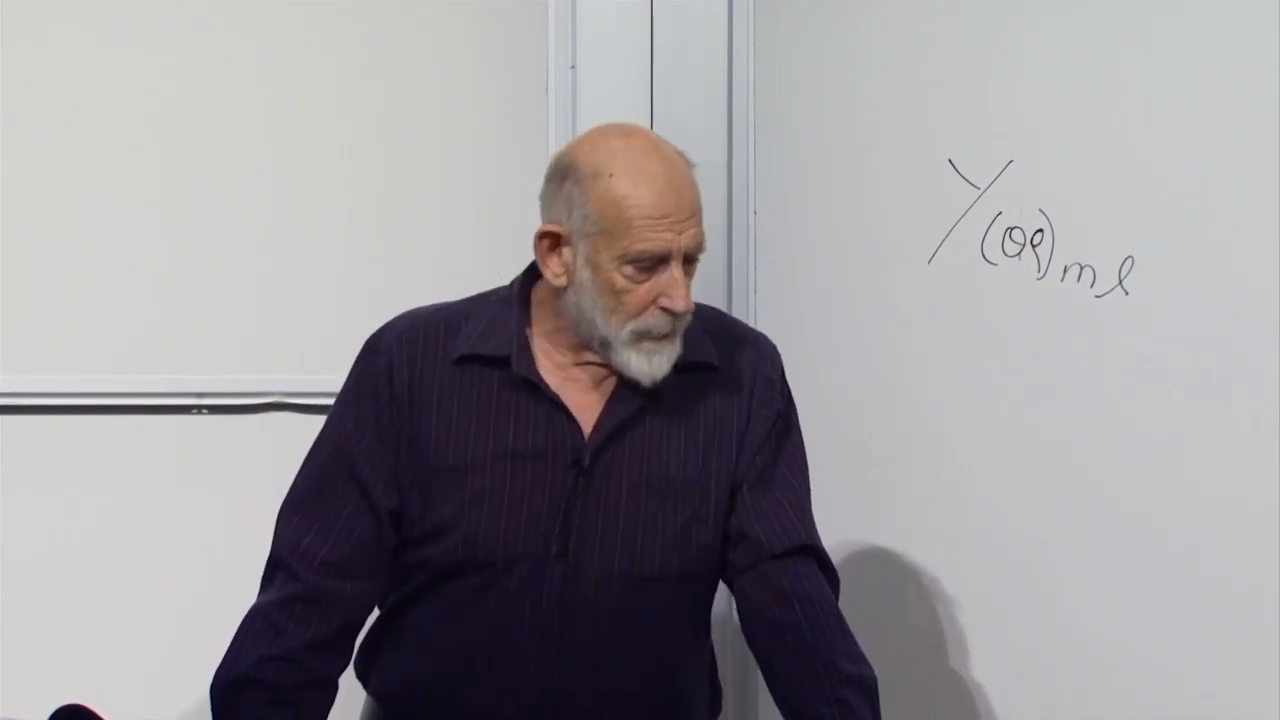
\includegraphics[width=0.9\linewidth]{lecture_03_frame_02.png}\caption{Với mômen động lượng cổ điển cố định, Hamiltonian xuyên tâm gồm động năng xuyên tâm, số hạng ly tâm \(L^2/(2mr^2)\) và thế tâm \(V(r)\).}\lectureframe{00:47:15}\end{figure}

Số hạng \(1/r^2\) là hàng rào ly tâm. Nó tăng lên khi hạt tiến gần gốc tọa độ, nên lực tương ứng hướng ra ngoài. Với các lực hút kiểu Coulomb đang xét, quỹ đạo có \(L\neq0\) sẽ lượn quanh tâm thay vì đi tới tâm. Khi \(L=0\), hàng rào không còn.

Với thế Coulomb hút,
\begin{equation}
V(r)=-\frac{\kappa}{r},
\end{equation}
số hạng ly tâm chiếm ưu thế khi \(r\) nhỏ, còn số hạng Coulomb giảm chậm hơn và chiếm ưu thế khi \(r\) lớn. Khi \(L\neq0\), tổng hai số hạng có một cực tiểu. Chuyển động tại cực tiểu có bán kính không đổi, nên là chuyển động tròn. Chuyển động liên kết với năng lượng cao hơn cực tiểu nhưng thấp hơn ngưỡng thoát dao động giữa bán kính nhỏ nhất và lớn nhất; trong bài toán Coulomb, đó là các dao động xuyên tâm của quỹ đạo elip.

\section{Phương trình xuyên tâm rút gọn}

Trong cơ học lượng tử, phần góc của trạng thái có mômen động lượng quỹ đạo xác định là một điều hòa cầu. Viết trạng thái đã tách biến dưới dạng
\begin{equation}
\Psi_{n_r\ell m}(r,\theta,\phi)
=\frac{u_{n_r\ell}(r)}{r}\,
Y_{\ell m}(\theta,\phi).
\end{equation}
Toán tử góc \(L^2\) có trị riêng
\begin{equation}
L^2Y_{\ell m}
=\hbar^2\ell(\ell+1)Y_{\ell m}.
\end{equation}
Với một cặp \(n_r,\ell\) cố định, viết gọn \(u_{n_r\ell}(r)\) thành \(u(r)\). Phương trình còn lại cho hàm xuyên tâm rút gọn là
\begin{equation}
\begin{aligned}
&-\frac{\hbar^2}{2m}\frac{d^2u}{dr^2}
+\frac{\hbar^2\ell(\ell+1)}{2mr^2}u(r)\\
&\qquad+V(r)u(r)=E_{n_r\ell}\,u(r).
\end{aligned}
\end{equation}

\editorialnote{Phương trình chỉ chứa đạo hàm bậc hai một chiều thuần túy sử dụng hàm xuyên tâm rút gọn \(u=rR\). Vì vậy, \(\psi(r)\) trong phương trình trên bảng của bài giảng tương ứng với \(u(r)\), còn thừa số xuyên tâm thông thường trong \(\Psi=R(r)Y_{\ell m}\) là \(R=u/r\). Quy ước này tránh xem \(-i\hbar\,d/dr\) như một toán tử động lượng xuyên tâm Hermite độc lập trên không gian Hilbert xuyên tâm ba chiều.}

Phương trình xuyên tâm rút gọn được trình bày trên bảng bên dưới.\footnote{Khung hình nguồn: \texttt{\detokenize{lecture_03_frame_03.png}}, tại \(00{:}54{:}32\) trong video bài giảng.}

\begin{figure}[htbp]\centering
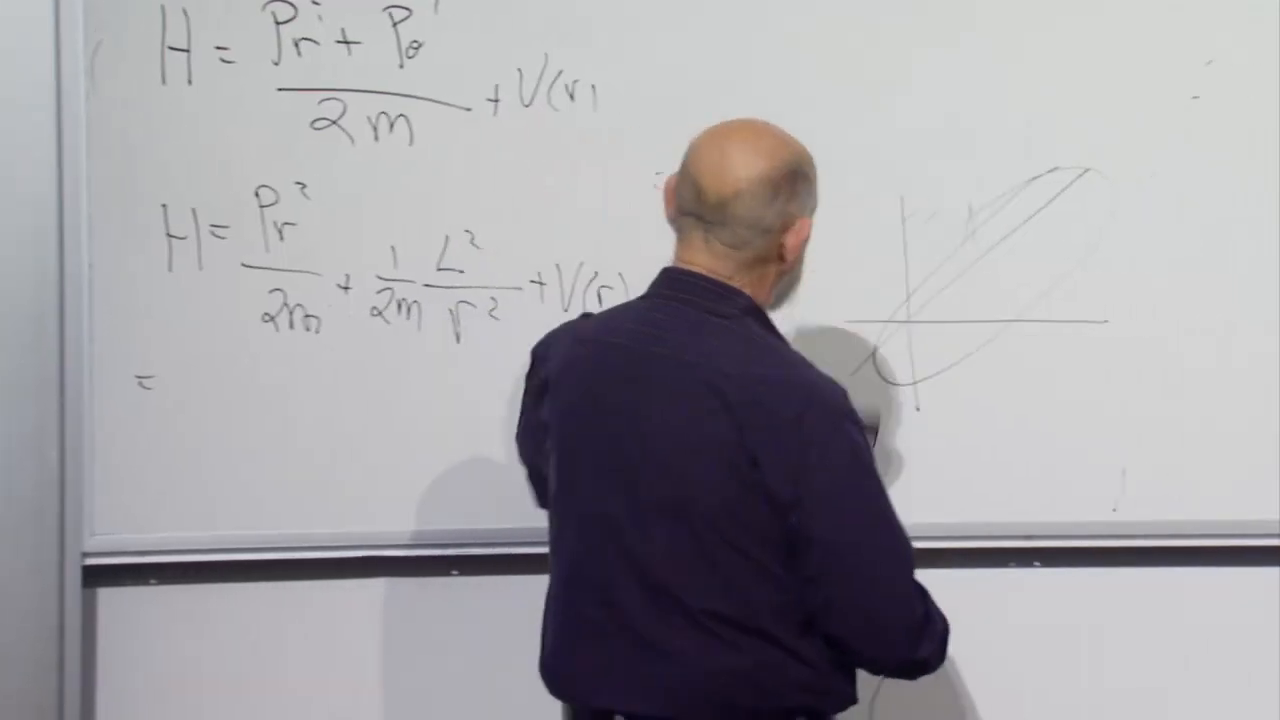
\includegraphics[width=0.9\linewidth]{lecture_03_frame_03.png}\caption{Với \(\ell\) cố định, hàm sóng xuyên tâm rút gọn thỏa mãn phương trình Schr\"odinger một chiều, có số hạng ly tâm tỷ lệ với \(\ell(\ell+1)/r^2\).}\lectureframe{00:54:32}\end{figure}

Cấu trúc góc ba chiều được gói gọn trong tham số \(\ell\). Số lượng tử từ \(m\) không xuất hiện trong phương trình xuyên tâm.

\begin{classroomqa}\lecturetimestamp{00:55:34}\audiencequestion{Với một \(\ell\) cho trước, \(2\ell+1\) trạng thái từ có cùng năng lượng không?}\lecturerresponse{Có, với điều kiện trạng thái riêng xuyên tâm cũng được giữ cố định. Với mỗi \(u_{n_r\ell}\) đã chọn, mọi giá trị \(m=-\ell,\ldots,\ell\) đều có cùng năng lượng vì \(m\) không xuất hiện trong phương trình xuyên tâm. Nói chung, các trạng thái riêng xuyên tâm khác nhau ứng với cùng \(\ell\) có năng lượng khác nhau.}\end{classroomqa}

\begin{classroomqa}\lecturetimestamp{00:56:03}\audiencequestion{Vì sao có thể thay \(L^2\) bằng \(\hbar^2\ell(\ell+1)\), và \(\ell\) liên hệ thế nào với các giá trị được phép của \(m\)?}\lecturerresponse{Số \(\ell\) dùng để ký hiệu một đa tuyến mômen động lượng và là giá trị \(m\) lớn nhất của nó. Mọi trạng thái trong đa tuyến đó đều có cùng trị riêng của \(L^2\), là \(\hbar^2\ell(\ell+1)\), nên ta thay trị riêng ấy vào phương trình xuyên tâm.}\end{classroomqa}

Các nghiệm tường minh bằng hàm đặc biệt không cần thiết cho lập luận hiện tại. Điều quan trọng là cách tổ chức các nghiệm.

\section{Nút xuyên tâm và các mức năng lượng}

Với \(\ell\) cố định, phương trình xuyên tâm rút gọn là một bài toán trị riêng thông thường một chiều. Các trạng thái liên kết được xếp theo số nút bên trong. Trạng thái xuyên tâm thấp nhất không có nút bên trong, trạng thái kế tiếp có một nút, còn trạng thái sau đó có hai nút. Nhiều nút hơn nghĩa là hàm sóng biến thiên nhanh hơn; hàm sóng biến thiên nhanh hơn thì động lượng lớn hơn, do đó động năng cũng lớn hơn.

Mỗi giá trị \(\ell\) xác định một toán tử xuyên tâm khác nhau vì số hạng ly tâm thay đổi theo \(\ell\). Do đó, các \(\ell=0,1,2,\ldots\) tạo thành những tháp mức xuyên tâm riêng biệt. Số hạng ly tâm dương đẩy các mức lên cao hơn khi mômen động lượng tăng. Mỗi trị riêng xuyên tâm ứng với \(\ell\) cố định đều có một đa tuyến từ với số chiều
\begin{equation}
2\ell+1.
\end{equation}
Các mức \(\ell=0\) là đơn tuyến, các mức \(\ell=1\) là tam tuyến, còn các mức \(\ell=2\) là ngũ tuyến. Đây là các độ suy biến do đối xứng quay bảo đảm; một đối xứng bổ sung cũng có thể khiến các trạng thái ứng với những giá trị \(\ell\) khác nhau suy biến cùng mức năng lượng.

Với các thế kiểu nguyên tử thỏa mãn \(V(r)\to0\) khi \(r\) lớn, quy ước chọn ngưỡng thoát là \(E=0\). Các trạng thái năng lượng âm tạo thành phổ liên kết rời rạc. Tại và phía trên \(E=0\), ta gặp phổ liên tục tán xạ. Nhận định này phụ thuộc vào hành vi của thế khi \(r\) lớn, và không áp dụng cho thế tâm giam hãm.

\section{Sự suy biến đặc biệt của thế Coulomb}

Thế Coulomb phi tương đối tính chính xác có thêm một sự trùng khớp giữa các mức năng lượng. Trạng thái xuyên tâm thấp nhất ứng với \(\ell=1\) có cùng năng lượng với trạng thái kích thích thứ nhất ứng với \(\ell=0\). Trạng thái \(\ell=1\) kế tiếp trùng mức với trạng thái kích thích thứ hai ứng với \(\ell=0\), còn trạng thái thấp nhất ứng với \(\ell=2\) cũng cùng mức với chúng. Quy luật này tiếp tục ở các tháp mức xuyên tâm và mômen động lượng cao hơn.

\begin{classroomqa}\lecturetimestamp{01:09:57}\audiencequestion{Sự suy biến Coulomb bổ sung này có cho thấy một đối xứng khác không?}\lecturerresponse{Có. Đây là một đối xứng bổ sung khác thường của thế Coulomb chính xác. Những thay đổi nhỏ của thế sẽ phá vỡ sự trùng khớp này; ta không trình bày cách suy ra nó ở đây.}\end{classroomqa}

Do đó, độ suy biến của các lớp vỏ quỹ đạo là
\begin{equation}
1,\qquad 4,\qquad 9,\qquad 16,\qquad \ldots
\end{equation}
trước khi tính đến spin electron.

\begin{classroomqa}\lecturetimestamp{01:11:46}\audiencequestion{Độ suy biến này mô tả nguyên tử hydro hay chỉ đúng với bài toán Coulomb lý tưởng?}\lecturerresponse{Nguyên tử hydro thỏa mãn kết quả này với độ chính xác rất cao, nhưng không hoàn toàn chính xác. Các hiệu chỉnh tương đối tính và kích thước hữu hạn của hạt nhân làm biến dạng quy luật Coulomb lý tưởng.}\end{classroomqa}

Hạt nhân điểm tạo ra thế \(1/r\) chính xác. Hạt nhân có điện tích phân bố trong một thể tích nhỏ tạo ra thế hơi khác khi electron xuyên vào thể tích đó; ngay cả sai khác nhỏ này cũng làm mất một phần suy biến đặc biệt.

Spin cũng chưa được tính đến. Nếu tính hai trạng thái spin của electron, số trạng thái trong mỗi lớp vỏ tăng gấp đôi, thành
\begin{equation}
2,\qquad 8,\qquad 18,\qquad 32,\qquad \ldots
\end{equation}
trước khi xét đến các độ tách mức bổ sung trong mô tả nguyên tử đầy đủ hơn.

\section{Trở lại phương trình Descartes}

Phương trình ban đầu dẫn đến bài toán xuyên tâm là phương trình Schr\"odinger ba chiều không phụ thuộc thời gian:
\begin{equation}
\begin{aligned}
-\frac{\hbar^2}{2m}\nabla^2\Psi+V(r)\Psi&=E\Psi,\\
\nabla^2&=\frac{\partial^2}{\partial x^2}
+\frac{\partial^2}{\partial y^2}
+\frac{\partial^2}{\partial z^2},\\
r&=\sqrt{x^2+y^2+z^2}.
\end{aligned}
\end{equation}
Chuyển sang tọa độ xuyên tâm và góc, rồi chọn một trạng thái riêng của \(L^2\).
Thay \(L^2\) bằng \(\hbar^2\ell(\ell+1)\) sẽ rút phương trình đạo hàm riêng thành phương trình vi phân thường theo tọa độ xuyên tâm đã nêu ở trên.

\begin{classroomqa}\lecturetimestamp{01:16:42}\audiencequestion{Có thể dùng những sai lệch so với phổ Coulomb lý tưởng để xác định kích thước hạt nhân không?}\lecturerresponse{Không thể chỉ dựa vào phép so sánh đơn giản này. Trước hết phải tính đến các hiệu chỉnh khác lớn hơn nhiều. Ở đây nhắc đến kích thước hạt nhân vì đó là ví dụ trực tiếp cho thấy thế Coulomb của hạt nhân điểm có thể sai khác như thế nào.}\end{classroomqa}

\begin{classroomqa}\lecturetimestamp{01:17:09}\audiencequestion{Khác biệt chính giữa số hạng mômen động lượng cổ điển và lượng tử là gì?}\lecturerresponse{Trong cơ học cổ điển, \(L^2\) là bình phương thông thường của độ lớn một vectơ được bảo toàn. Trong một đa tuyến quỹ đạo lượng tử, trị riêng của nó là \(\hbar^2\ell(\ell+1)\), chứ không đơn giản là \(\hbar^2\ell^2\). Số hạng bổ sung xuất hiện do các thành phần mômen động lượng không giao hoán với nhau.}\end{classroomqa}

\begin{classroomqa}\lecturetimestamp{01:17:58}\audiencequestion{Hàm sóng của trạng thái liên kết có miền hỗ trợ compact không?}\lecturerresponse{Không. Chúng vươn ra xa tâm tùy ý. Với các trạng thái liên kết nguyên tử đang xét, biên độ giảm theo hàm mũ ở khoảng cách lớn, nên xác suất trở nên không đáng kể nhưng không triệt tiêu bên ngoài bất kỳ bán kính hữu hạn nào.}\end{classroomqa}

\begin{classroomqa}\lecturetimestamp{01:18:48}\audiencequestion{Khi \(\ell=0\) làm mất giếng ly tâm, điểm cân bằng ổn định sẽ ra sao?}\lecturerresponse{Không còn cực tiểu do sự cạnh tranh giữa hàng rào ly tâm và lực hút tạo ra. Trong mô hình lý tưởng Coulomb điểm, chuyển động cổ điển hướng về tâm kỳ dị. Trong cơ học lượng tử, trạng thái thấp nhất không thể đồng thời có vị trí xác định chính xác tại tâm và động lượng bằng không, nên hàm sóng thấp nhất có độ trải rộng không gian hữu hạn.}\end{classroomqa}

\editorialnote{Với thế tâm chính quy, quỹ đạo cổ điển có mômen động lượng bằng không có thể tiếp tục đi qua gốc tọa độ. Còn với thế Coulomb điểm lý tưởng, \(r=0\) là một điểm kỳ dị va chạm; muốn tiếp tục quỹ đạo cổ điển thì cần thêm một quy tắc xác định.}

Phép rút gọn cổ điển đặt một quỹ đạo duy nhất vào một mặt phẳng, nhưng không thể áp dụng tương tự cho hàm sóng lượng tử. Một trạng thái quỹ đạo lượng tử trải rộng trong không gian ba chiều. Toán tử góc đầy đủ là \(L^2=L_x^2+L_y^2+L_z^2\), và trị riêng của nó giữ nguyên kết quả ba chiều \(\hbar^2\ell(\ell+1)\).

\begin{classroomqa}\lecturetimestamp{01:21:30}\audiencequestion{Vì sao bài toán lượng tử vẫn là bài toán ba chiều sau khi quỹ đạo cổ điển đã được đặt vào một mặt phẳng?}\lecturerresponse{Chỉ quỹ đạo cổ điển được đặt vào một mặt phẳng cố định bằng cách chọn hệ tọa độ vuông góc với vectơ mômen động lượng bảo toàn của nó. Hàm sóng lượng tử tồn tại trong không gian ba chiều. Các thành phần mômen động lượng còn lại vẫn hiện diện thông qua \(L^2\), đó là lý do phương trình xuyên tâm chứa \(\ell(\ell+1)\) chứ không chỉ chứa bình phương của một thành phần duy nhất.}\end{classroomqa}

\begin{classroomqa}\lecturetimestamp{01:22:54}\audiencequestion{Mọi bài toán lượng tử đều có toán tử nâng và hạ không?}\lecturerresponse{Không. Chúng chỉ xuất hiện trong một số trường hợp đặc biệt thuận lợi. Mômen động lượng là một trường hợp như vậy, và dao động tử điều hòa là một trường hợp khác. Trường hợp dao động tử đặc biệt hữu ích vì chuyển động quanh một cân bằng bền thường gần đúng là dao động điều hòa, kể cả các dao động xuyên tâm nhỏ quanh cực tiểu của thế hiệu dụng.}\end{classroomqa}

Đến đây, ta tạm gác bài toán nguyên tử và chuyển sang dao động tử điều hòa, ví dụ tiếp theo về phổ được xác định bằng các toán tử bậc thang.

\section{Dao động nhỏ và dao động tử điều hòa}

Gần một vị trí cân bằng bền, một độ dời đủ nhỏ thường tạo ra dao động điều hòa. Thế xuyên tâm hiệu dụng khi mômen động lượng khác không là một ví dụ: chuyển động xuyên tâm gần đáy giếng thế gần đúng là dao động điều hòa.

Xét dao động tử một chiều có khối lượng bằng đơn vị. Gọi \(x\) là độ dời so với vị trí cân bằng và viết hằng số lò xo dưới dạng \(k=\omega^2\). Hamiltonian cổ điển là
\begin{equation}
H=\frac{p^2}{2}+\frac{\omega^2x^2}{2}.
\end{equation}
Các phương trình Hamilton cho
\begin{equation}
\dot{x}=\frac{\partial H}{\partial p}=p,
\qquad
\dot{p}=-\frac{\partial H}{\partial x}=-\omega^2x,
\end{equation}
và do đó
\begin{equation}
\ddot{x}=-\omega^2x.
\end{equation}
Vậy \(\omega\) là tần số dao động cổ điển.

\section{Phân tích thành nhân tử và năng lượng điểm không}

Trong cơ học lượng tử,
\begin{equation}
[x,p]=i\hbar.
\end{equation}
Hamiltonian là tổng các bình phương, gợi ý cách phân tích thành nhân tử sau:
\begin{align}
\frac{1}{2}(p+i\omega x)(p-i\omega x)
&=\frac{1}{2}\left(p^2+\omega^2x^2+i\omega[x,p]\right) \\
&=\frac{1}{2}\left(p^2+\omega^2x^2-\hbar\omega\right).
\end{align}
Do đó,
\begin{equation}
H=\frac{1}{2}(p+i\omega x)(p-i\omega x)
+\frac{1}{2}\hbar\omega.
\end{equation}
Số hạng cộng thêm \(\hbar\omega/2\) là năng lượng điểm không.

Trong cơ học cổ điển, năng lượng thấp nhất đạt được khi \(x=p=0\). Trong cơ học lượng tử, không trạng thái nào có thể đồng thời xác định chính xác cả vị trí lẫn động lượng tại không. Hơn nữa, hai số hạng \(p^2/2\) và \(\omega^2x^2/2\) đều dương và không thể triệt tiêu lẫn nhau. Vì vậy, năng lượng trạng thái cơ bản khác không là điều không thể tránh khỏi.

Trong phép tính dùng thang toán tử, tạm thời có thể bỏ qua hằng số cộng chung rồi khôi phục lại ở cuối.

\begin{classroomqa}\lecturetimestamp{01:36:10}\audiencequestion{Dấu dương của số hạng năng lượng điểm không có cho ta biết thêm điều gì không?}\lecturerresponse{Hamiltonian của dao động tử là toán tử dương: nó là tổng các bình phương dương, nên năng lượng không thể âm.}\end{classroomqa}

\section{Thang dao động tử}

Đưa vào các toán tử không thứ nguyên\footnote{Trong đoạn \(01{:}37\)--\(01{:}42\), phép tính dùng \(\hbar=1\). Trong các định nghĩa đã chuẩn hóa dưới đây, thừa số \(\hbar\) được khôi phục để \(A_\pm\) không thứ nguyên và giao hoán tử của chúng bằng đơn vị.}
\begin{equation}
A_+=\frac{p+i\omega x}{\sqrt{2\hbar\omega}},
\qquad
A_-=\frac{p-i\omega x}{\sqrt{2\hbar\omega}}.
\end{equation}
Chúng là các toán tử liên hợp Hermite:
\begin{equation}
A_+^\dagger=A_-.
\end{equation}
Giao hoán tử của chúng là
\begin{align}
[A_-,A_+]
&=\frac{1}{2\hbar\omega}
\left([p,i\omega x]+[-i\omega x,p]\right) \\
&=1.
\end{align}

Định nghĩa
\begin{equation}
N=A_+A_-.
\end{equation}
Khi đó, Hamiltonian là
\begin{equation}
H=\hbar\omega\left(N+\frac{1}{2}\right).
\end{equation}
Vì thế, việc tìm phổ năng lượng quy về tìm các trị riêng của \(N\).

Giả sử
\begin{equation}
N|n\rangle=n|n\rangle.
\end{equation}
Các giao hoán tử với \(N\) là\footnote{Các bước trung gian tại \(01{:}45{:}37\)--\(01{:}48{:}10\) được dựng lại trực tiếp từ các hệ thức đã nêu \(N=A_+A_-\) và \([A_-,A_+]=1\).}
\begin{align}
[N,A_+]
&=A_+[A_-,A_+]=A_+, \\
[N,A_-]
&=[A_+,A_-]A_-=-A_-.
\end{align}
Suy ra
\begin{align}
N\bigl(A_+|n\rangle\bigr)
&=(n+1)A_+|n\rangle, \\
N\bigl(A_-|n\rangle\bigr)
&=(n-1)A_-|n\rangle.
\end{align}
Vậy \(A_+\) làm tăng trị riêng của \(N\) thêm một đơn vị, còn \(A_-\) làm giảm nó đi một đơn vị, miễn là vectơ thu được khác không.

Toán tử \(N\) không âm:
\begin{equation}
\langle\psi|N|\psi\rangle
=\langle\psi|A_+A_-|\psi\rangle
=\|A_-|\psi\rangle\|^2
\geq0.
\end{equation}
Vì vậy, quá trình hạ không thể tiếp tục đến các trị riêng âm. Ở trạng thái đáy \(|b\rangle\), quá trình phải kết thúc:
\begin{equation}
A_-|b\rangle=0.
\end{equation}

Với các trạng thái riêng đã chuẩn hóa, chuẩn của chúng xác định các hệ số trong thang:
\begin{align}
\|A_-|n\rangle\|^2
&=\langle n|A_+A_-|n\rangle=n, \\
\|A_+|n\rangle\|^2
&=\langle n|A_-A_+|n\rangle=n+1.
\end{align}
Do đó, có thể chọn pha sao cho
\begin{equation}
A_-|n\rangle=\sqrt{n}\,|n-1\rangle,
\qquad
A_+|n\rangle=\sqrt{n+1}\,|n+1\rangle.
\end{equation}

\begin{classroomqa}\lecturetimestamp{01:52:42}\audiencequestion{Nếu \(A_-\) hạ một trạng thái rồi \(A_+\) nâng nó trở lại, thì \(A_+A_-\) tạo ra trị riêng \(n\) như thế nào?}\lecturerresponse{Tác dụng của các toán tử bậc thang có kèm theo các thừa số chuẩn hóa. Tác dụng trước hết của \(A_-\) cho thừa số \(\sqrt n\), còn tác dụng của \(A_+\) lên trạng thái thu được cho thêm thừa số \(\sqrt n\). Tích của chúng là \(n\).}\end{classroomqa}

Thật vậy,
\begin{equation}
A_+A_-|n\rangle
=\sqrt n\,A_+|n-1\rangle
=n|n\rangle.
\end{equation}

\begin{classroomqa}\lecturetimestamp{01:55:52}\audiencequestion{Trị riêng thấp nhất của \(N\) nhất thiết bằng không, hay có thể dương?}\lecturerresponse{Nó phải bằng không, và phổ của \(N\) gồm các số nguyên không âm. Tuy nhiên, ta chưa đưa ra chứng minh cho kết luận về đầu mút này.}\end{classroomqa}

\editorialnote{Gọi \(|b\rangle\) là trạng thái thấp nhất. Vì phép hạ phải kết thúc nên \(A_-|b\rangle=0\). Suy ra ngay \(N|b\rangle=A_+A_-|b\rangle=0\), do đó trị riêng thấp nhất của \(N\) bằng không.}

Bắt đầu từ trạng thái thấp nhất này rồi áp dụng \(A_+\), ta được
\begin{equation}
n=0,1,2,\ldots.
\end{equation}
Khôi phục số hạng cộng thêm điểm không, các mức năng lượng của dao động tử là
\begin{equation}
E_n=\hbar\omega\left(n+\frac{1}{2}\right),
\qquad n=0,1,2,\ldots.
\end{equation}

Đại số dao động tử sẽ được triển khai thêm và dùng để giải các bài toán lượng tử khác.
\chapter{Hàm sóng của dao động tử, spin một phần hai và sự trao đổi hạt}

\section{Dao động tử ở khắp nơi}

Mọi hệ có trạng thái cân bằng bền đều có thể dao động khi bị dịch chuyển khỏi trạng thái cân bằng đó. Hệ có thể có một hoặc nhiều tần số. Chẳng hạn, dây đàn violin có mode cơ bản và các họa âm bậc cao. Khi gảy dây, ta kích thích một tổ hợp các mode ấy.

Những ví dụ quan trọng hơn ở đây là các trường. Cấu hình cân bằng của trường điện từ là chân không: không có điện trường, không có từ trường và không có dao động điện từ. Đưa bức xạ vào một hốc cộng hưởng hoặc ống dẫn sóng thì trường có thể dao động ở các mode được phép, mỗi mode có tần số riêng. Trong lý thuyết lượng tử, các mode ấy mô tả những tập hợp photon.

Ý tưởng tương tự cũng áp dụng cho tinh thể. Hình dung mỗi nguyên tử là một dao động tử độc lập sẽ gây hiểu lầm. Các nguyên tử tác dụng lực lên nhau, nên khi một nguyên tử dịch chuyển, các nguyên tử lân cận cũng bị ảnh hưởng và một sóng lan truyền qua tinh thể. Các mode chuẩn của chuyển động liên kết đó là những dao động tử điều hòa, còn lượng tử của chúng được gọi là phonon. Photon và phonon là những đối tượng vật lý khác nhau, nhưng cả hai đều dẫn trở lại cùng một đại số dao động tử.

\section{Đại số dao động tử}

Trong phần bàn về dao động tử, lấy khối lượng và hằng số Planck rút gọn bằng một:
\[
m=1,\qquad \hbar=1.
\]
Hamiltonian là
\begin{equation}
H=\frac{p^{2}}{2}+\frac{\omega^{2}x^{2}}{2}.
\end{equation}
Tham số \(\omega\) xác định độ cong của thế năng, đồng thời cũng là tần số dao động.

Định nghĩa các toán tử nâng và hạ như sau:
\begin{equation}
A_{\pm}=\frac{p\pm i\omega x}{\sqrt{2\omega}}.
\end{equation}
Chọn chuẩn hóa sao cho
\begin{equation}
[A_{-},A_{+}]=1.
\end{equation}
Toán tử số là
\begin{equation}
N=A_{+}A_{-}.
\end{equation}
Các phương trình này cùng suy ra rằng \(A_{+}\) làm tăng một đơn vị trị riêng của \(N\), còn \(A_{-}\) làm giảm trị riêng đó một đơn vị. Phổ thu được là
\begin{equation}
n=0,1,2,3,\ldots .
\end{equation}

Nhân hai toán tử bậc thang với nhau cũng cho thấy hiệu chỉnh lượng tử đối với năng lượng cổ điển:
\begin{align}
N
&=\frac{1}{2\omega}(p+i\omega x)(p-i\omega x)\\
&=\frac{1}{2\omega}\left(p^{2}+\omega^{2}x^{2}
 +i\omega[x,p]\right)\\
&=\frac{1}{2\omega}\left(p^{2}+\omega^{2}x^{2}-\omega\right),
\end{align}
trong đó \([x,p]=i\). Do đó,
\begin{equation}
H=\omega\left(N+\frac12\right).
\end{equation}
Nếu hằng số cộng không liên quan đến bài toán, ta có thể dùng Hamiltonian đã dịch:
\begin{equation}
H_{\mathrm{shifted}}=H-\frac{\omega}{2}=\omega N.
\end{equation}
Số hạng \(\omega/2\) là năng lượng điểm không, hay năng lượng trạng thái cơ bản, của dao động tử. Với một mode trường, số hạng tương tự được gọi là năng lượng chân không. Nó phản ánh nguyên lý bất định: không trạng thái nào có thể đồng thời có \(x\) và \(p\) bằng không một cách xác định, nên cả hai số hạng bậc hai dương trong \(H\) không thể cùng có giá trị kỳ vọng bằng không.

\begin{classroomqa}
\lecturetimestamp{00:09:46}
\audiencequestion{Vì sao số không được tính vào phổ của toán tử số?}
\lecturerresponse{Có thể chứng minh điều này một cách tường minh bằng cách dựng hàm sóng trạng thái cơ bản. Phép dựng đó sẽ cho thấy có một trạng thái thỏa \(N=0\).}
\end{classroomqa}

Để bắt đầu phép dựng ấy, thay các vectơ trạng thái bằng các hàm sóng theo vị trí. Các trạng thái riêng năng lượng trở thành
\[
\psi_{0}(x),\ \psi_{1}(x),\ \psi_{2}(x),\ldots,
\]
và các toán tử cơ bản tác dụng như sau:
\begin{equation}
X\longmapsto x,\qquad
P\longmapsto -i\frac{d}{dx}.
\end{equation}
Khi khôi phục \(\hbar\), phép thay thứ hai sẽ là
\(P\mapsto-i\hbar\,d/dx\).

Trước khi giải tìm \(\psi_{0}\), ta có thể trả lời câu hỏi bằng lập luận trừu tượng nhanh hơn. Trên thang rời rạc gồm các trạng thái riêng chuẩn hóa được của dao động tử, \(N=A_{+}A_{-}\) không âm, nên không thể tiếp tục hạ liên tiếp từng đơn vị mãi mãi. Ở điểm cuối---mà hàm sóng chuẩn hóa được sẽ được dựng bên dưới---, phải có một trạng thái, ký hiệu là \(\lvert0\rangle\), sao cho
\begin{equation}
A_{-}\lvert0\rangle=\mathbf 0.
\end{equation}
Nếu không thì \(A_{-}\lvert0\rangle\) sẽ là một trạng thái khác thấp hơn một bậc. Suy ra ngay rằng
\begin{equation}
N\lvert0\rangle
=A_{+}A_{-}\lvert0\rangle
=\mathbf 0
=0\,\lvert0\rangle.
\end{equation}
Vậy trạng thái thấp nhất có trị riêng số bằng không.

\begin{classroomqa}
\lecturetimestamp{00:14:57}
\audiencequestion{Nếu trị riêng bằng không, vế phải có nên chứa một vectơ riêng không?}
\lecturerresponse{Ket \(\lvert0\rangle\) là một vectơ chuẩn hóa khác không có nhãn bằng không. Trong \(N\lvert0\rangle=0\,\lvert0\rangle\), vế phải là vectơ không. Ket trạng thái cơ bản và vectơ không là hai đối tượng khác nhau.}
\end{classroomqa}

\section{Phương trình Schr\"odinger và các nghiệm vật lý}

Giờ hãy trở lại biểu diễn theo vị trí. Phương trình Schr\"odinger không phụ thuộc thời gian là
\begin{equation}
\left[
-\frac12\frac{d^{2}}{dx^{2}}
+\frac12\omega^{2}x^{2}
\right]\psi(x)=E\psi(x).
\end{equation}
Là một phương trình vi phân bậc hai, nó có các nghiệm hình thức ứng với mọi giá trị \(E\). Phần lớn các nghiệm hình thức ấy không phải là trạng thái vật lý của dao động tử. Chúng tăng theo hàm mũ khi \(\lvert x\rvert\) lớn, khiến chuẩn của chúng phân kỳ.

Với một trạng thái liên kết, hàm sóng phải bình phương khả tích:
\begin{equation}
\int_{-\infty}^{\infty}\psi^{*}(x)\psi(x)\,dx<\infty.
\end{equation}
Sau đó có thể chuẩn hóa hàm sóng để tích phân bằng một. Chỉ những giá trị năng lượng đặc biệt mới cho các nghiệm như vậy. Các trạng thái vị trí và động lượng trên đường thẳng vô hạn là những trường hợp ngoại lệ về mặt này, còn các nghiệm dao động tử tăng theo hàm mũ thì đơn giản là bị loại khỏi không gian trạng thái.

\section{Trạng thái cơ bản dạng Gaussian}

Có thể giải phương trình bậc hai, nhưng đại số bậc thang cho một phương trình bậc nhất đơn giản hơn:
\begin{equation}
A_{-}\psi_{0}(x)=0.
\end{equation}
Khi vế phải bằng không, hệ số tổng thể trong \(A_{-}\) không ảnh hưởng, nên phương trình này tương đương với
\begin{equation}
(p-i\omega x)\psi_{0}(x)=0.
\end{equation}
Dùng \(p=-i\,d/dx\), ta được
\begin{equation}
\left(\frac{d}{dx}+\omega x\right)\psi_{0}(x)=0.
\end{equation}

\begin{classroomqa}
\lecturetimestamp{00:22:32}
\audiencequestion{Có thể giải phương trình này bằng phương pháp phân ly biến số không?}
\lecturerresponse{Ở đây chỉ có một biến độc lập, nên không có hai biến để phân ly. Viết dưới dạng \(\psi_{0}'/\psi_{0}=-\omega x\), phương trình có dạng của một đạo hàm logarithm. Điều đó gợi ý biểu diễn hàm sóng dưới dạng hàm mũ.}
\end{classroomqa}

Một cách giải hữu ích là đặt
\begin{equation}
\psi_{0}(x)=e^{f(x)}.
\end{equation}
Khi đó,
\[
\psi_{0}'(x)=f'(x)e^{f(x)},
\]
và thừa số hàm mũ chung triệt tiêu. Phương trình rút gọn thành
\begin{equation}
\frac{df}{dx}+\omega x=0.
\end{equation}

\begin{classroomqa}
\lecturetimestamp{00:26:28}
\audiencequestion{Trong \(f(x)\) có nên có dấu trừ không?}
\lecturerresponse{Có. Vì \(df/dx=-\omega x\), phép tích phân cho một số hạng bậc hai mang dấu âm.}
\end{classroomqa}

Do đó,
\begin{equation}
f(x)=-\frac12\omega x^{2}+C,
\end{equation}
và
\begin{equation}
\psi_{0}(x)\propto e^{-\omega x^{2}/2}.
\end{equation}
Ta chưa xác định hằng số nhân chuẩn hóa. Điều quan trọng là dạng Gaussian: hàm này trơn, tập trung gần gốc tọa độ và giảm nhanh khi \(\lvert x\rvert\) lớn. Rõ ràng nó bình phương khả tích.

Không cần thế đáp án trở lại phương trình bậc hai để tìm năng lượng. Đại số đã cho ta
\begin{equation}
E_{0}=\frac{\omega}{2}.
\end{equation}

\section{Trạng thái kích thích, nút và chuyển động cổ điển}

Trạng thái kích thích thứ nhất thu được bằng cách nâng trạng thái cơ bản:
\begin{equation}
\psi_{1}(x)\propto A_{+}\psi_{0}(x)
\propto(p+i\omega x)e^{-\omega x^{2}/2}.
\end{equation}
Phương trình trạng thái cơ bản cho biết
\[
p\psi_{0}=i\omega x\,\psi_{0}.
\]
Đổi dấu trong toán tử bậc thang biến sự triệt tiêu thành phép cộng:
\begin{equation}
(p+i\omega x)\psi_{0}
=2i\omega x\,\psi_{0}.
\end{equation}
Bỏ qua một hằng số tổng thể,
\begin{equation}
\psi_{1}(x)\propto x\,e^{-\omega x^{2}/2}.
\end{equation}

Hàm sóng này là hàm lẻ:
\begin{equation}
\psi_{1}(-x)=-\psi_{1}(x).
\end{equation}
Mật độ xác suất của nó là hàm chẵn, nhưng có một nút tại gốc tọa độ:
\begin{equation}
\lvert\psi_{1}(0)\rvert^{2}=0.
\end{equation}
Vậy mật độ xác suất của trạng thái kích thích thứ nhất có một nút tại \(x=0\).

Tác dụng lặp lại của \(A_{+}\) cho các đa thức bậc cao hơn nhân với cùng một bao Gaussian.\footnote{Bài giảng nêu các thừa số đa thức bậc cao, nút bổ sung ở mỗi bước và tính chẵn lẻ luân phiên từ \(00{:}34{:}25\) đến \(00{:}35{:}49\). Dạng tích của Gaussian với đa thức được Leonard Susskind và Art Friedman xác nhận trong \emph{Cơ học lượng tử: Những kiến thức tối thiểu} (2014), ở phần bàn về các hàm riêng của dao động tử.} Bỏ qua chuẩn hóa,
\begin{equation}
\psi_{n}(x)=P_{n}(x)e^{-\omega x^{2}/2}.
\end{equation}
Tính chẵn lẻ luân phiên giữa chẵn và lẻ, và mỗi bước làm tăng thêm một nút. Khi \(n\) tăng, hàm sóng trải rộng ra xa gốc hơn và dao động nhanh hơn.

Hai đặc điểm này có ý nghĩa vật lý trực tiếp. Hàm sóng có biên độ đáng kể ở xa gốc hơn tương ứng với thế năng lớn hơn, vì thế năng tăng theo \(x^{2}\). Dao động nhanh trong không gian vị trí báo hiệu động lượng lớn hơn. Một dao động tử kích thích mạnh có khả năng vươn xa tâm hơn; khi đi qua vùng trung tâm, nó mang động lượng lớn hơn và hàm sóng dao động nhanh hơn ở vùng đó.

\begin{classroomqa}
\lecturetimestamp{00:37:18}
\audiencequestion{Khi \(n\) lớn, dao động tử điều hòa có tiến gần đến hành vi cổ điển không?}
\lecturerresponse{Chuyển động cổ điển không được biểu diễn bởi một trạng thái riêng năng lượng dừng duy nhất. Nó xuất hiện trong một gói sóng gồm nhiều mức năng lượng. Chẳng hạn, một Gaussian bị dịch chuyển tiến hóa qua lại như một dao động tử cổ điển, và độ bất định tương đối giảm khi biên độ dao động tăng.}
\end{classroomqa}

Bắt đầu với Gaussian của trạng thái cơ bản rồi dịch chuyển nó khỏi gốc. Gói sóng sau khi dịch chuyển không còn là trạng thái riêng năng lượng nữa; nó là chồng chập của nhiều trạng thái như vậy. Theo phương trình Schr\"odinger phụ thuộc thời gian, các thành phần của gói sóng thu được những pha khác nhau. Gói sóng dao động từ bên này sang bên kia của thế năng, phát triển biến thiên pha nhanh gần tâm và trở nên trơn trở lại gần điểm quay. Biên độ dao động càng lớn so với độ rộng của gói sóng thì chuyển động biểu hiện càng gần với chuyển động cổ điển.

\begin{classroomqa}
\lecturetimestamp{00:39:29}
\audiencequestion{Hàm sóng của trạng thái kích thích thứ hai có đi qua không tại gốc tọa độ không?}
\lecturerresponse{Không. Thừa số đa thức của nó không chỉ gồm \(x^{2}\); nó còn chứa một số hạng hằng, nên hàm sóng không nhất thiết triệt tiêu tại \(x=0\).}
\end{classroomqa}

Lập luận bậc thang cũng giả định rằng \(A_{+}\) và \(A_{-}\) là các toán tử liên hợp Hermite trên miền dao động tử gồm các hàm bình phương khả tích, với điều kiện biên cần thiết để quan hệ liên hợp đúng. Các nghiệm hình thức tăng theo hàm mũ không thuộc miền đó.

\begin{classroomqa}
\lecturetimestamp{00:40:45}
\audiencequestion{Có cách tổng quát nào để nhận biết một Hamiltonian có thể giải được bằng các phương pháp đại số hay không?}
\lecturerresponse{Không có quy tắc tổng quát như vậy. Các ví dụ giải được chính xác rất hiếm. Dao động tử điều hòa và nguyên tử hydro phi tương đối tính lý tưởng là những trường hợp may mắn mà các phương pháp đại số có hiệu quả.}
\end{classroomqa}

\section{Spin một phần hai như động lượng góc}

Spin là động lượng góc do hạt mang, độc lập với chuyển động quỹ đạo của khối tâm. Hạt đứng yên không có động lượng góc quỹ đạo \(\mathbf R\times\mathbf P\), nhưng vẫn có thể có spin. Có thể thử hình dung hạt như một vật nhỏ đang quay, hoặc xem spin là một tính chất lượng tử nội tại. Phát biểu quyết định mang tính toán học: các thành phần spin biến đổi dưới phép quay không gian và tuân theo các hệ thức giao hoán của động lượng góc.

Từ đây trở đi, khôi phục \(\hbar\). Các thành phần động lượng góc thỏa mãn
\begin{equation}
[L_{z},L_{x}]=i\hbar L_{y},
\end{equation}
Hai hệ thức còn lại thu được bằng cách hoán vị vòng. Các ma trận Pauli không thứ nguyên là
\begin{equation}
\begin{aligned}
\sigma_{z}&=
\begin{pmatrix}
1&0\\
0&-1
\end{pmatrix},\\[0.4em]
\sigma_{x}&=
\begin{pmatrix}
0&1\\
1&0
\end{pmatrix},\\[0.4em]
\sigma_{y}&=
\begin{pmatrix}
0&-i\\
i&0
\end{pmatrix}.
\end{aligned}
\end{equation}
Trong cơ sở này, \(\sigma_{z}\) là ma trận đường chéo. Các trị riêng của nó là \(+1\) và
\(-1\).

\begin{classroomqa}
\lecturetimestamp{00:47:35}
\audiencequestion{Trong \(\sigma_x\) có dấu trừ không?}
\lecturerresponse{Không. Hai phần tử ngoài đường chéo của \(\sigma_x\) đều dương.}
\end{classroomqa}

Phép tính trên bảng tại \(00{:}49{:}35\) bắt đầu quá trình nhân từng phần tử.
Thực hiện đầy đủ các phép nhân, ta được
\begin{align}
\sigma_{z}\sigma_{x}
&=
\begin{pmatrix}
0&1\\
-1&0
\end{pmatrix}
=i\sigma_{y},\\
\sigma_{x}\sigma_{z}
&=
\begin{pmatrix}
0&-1\\
1&0
\end{pmatrix}
=-i\sigma_{y}.
\end{align}
Do đó,
\begin{equation}
[\sigma_{z},\sigma_{x}]=2i\sigma_{y}.
\end{equation}
Thừa số hai dư ra được loại bỏ bằng cách định nghĩa các toán tử spin vật lý như sau:\footnote{Phép tính trên bảng bỏ qua \(\hbar\). Ở đây khôi phục đại lượng này để \(S_i\) có đơn vị động lượng góc.}
\begin{equation}
S_{i}=\frac{\hbar}{2}\sigma_{i}.
\end{equation}
Khi đó,
\begin{equation}
[S_{z},S_{x}]=i\hbar S_{y},
\end{equation}
và tương tự với các phép hoán vị vòng. Vì vậy, một nửa các ma trận Pauli, sau khi khôi phục thừa số \(\hbar\), tạo thành một hệ động lượng góc.

Đặt \(\hbar=1\) thì thu được dạng trình bày dưới đây.\footnote{Khung nguồn là \texttt{bài giảng\_04\_khung\_02.png}.}
\begin{figure}[htbp]
\centering
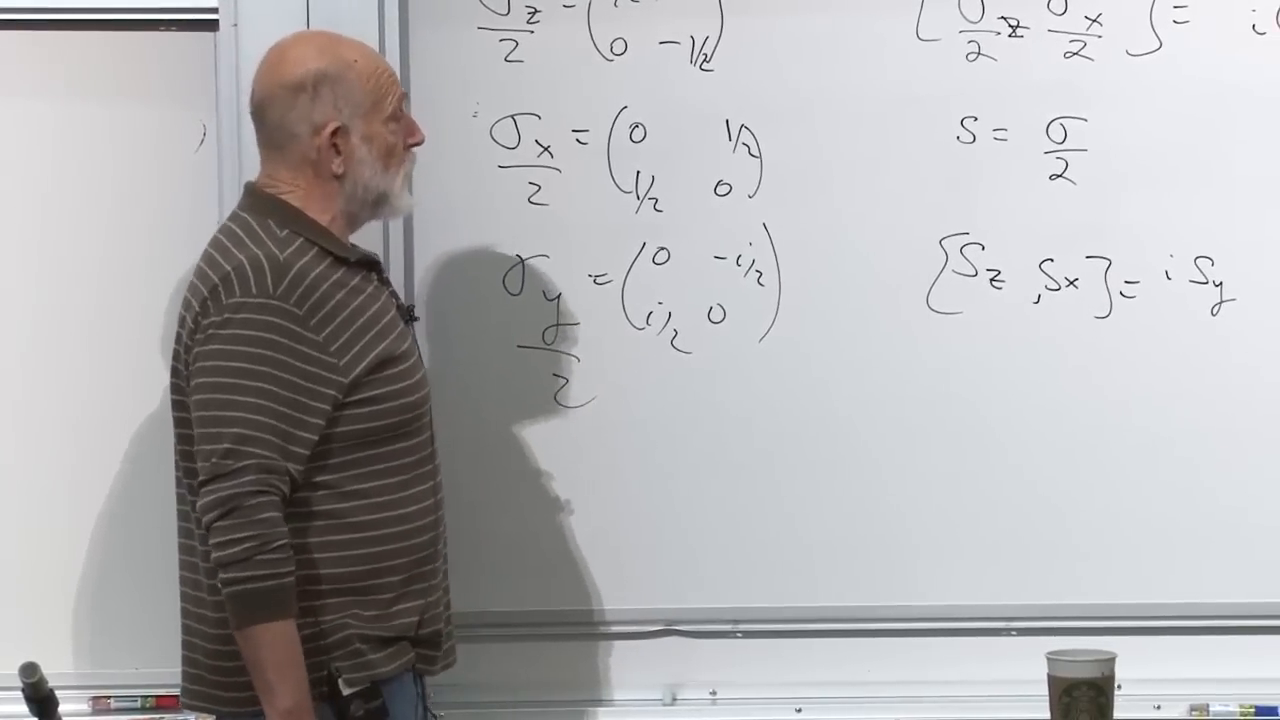
\includegraphics[width=0.9\linewidth]{lecture_04_frame_02.png}
\caption{Trong đơn vị \(\hbar=1\), một nửa các ma trận Pauli là các toán tử động lượng góc spin một phần hai và thỏa mãn \([S_z,S_x]=iS_y\).}
\lectureframe{00:55:41}
\end{figure}

Hai phương trình trị riêng \(S_z\) là
\begin{equation}
S_z\lvert\pm\rangle
=\pm\frac{\hbar}{2}\lvert\pm\rangle.
\end{equation}
Tương đương, số lượng tử từ không thứ nguyên là
\begin{equation}
m_{s}=\pm\frac12,
\qquad
S_{z}\lvert m_{s}\rangle
=m_{s}\hbar\,\lvert m_{s}\rangle.
\end{equation}
Các toán tử nâng và hạ của động lượng góc dịch chuyển \(m\) theo các bước nguyên, nhưng điều đó không có nghĩa là mọi thang đều phải đi qua số không. Các đa tuyến nguyên chứa các giá trị \(m\) nguyên, còn các đa tuyến bán nguyên chứa các giá trị bán nguyên. Với spin một phần hai, thang chỉ có hai thành viên \(m_s=+1/2\) và \(m_s=-1/2\).

Hai trạng thái này tạo thành bộ đôi spin một phần hai. Electron, muon, neutrino và quark là những hạt thuộc các đa tuyến spin bán nguyên như vậy.

\section{Động lượng góc quỹ đạo và spin}

Giờ đây ta có hai loại động lượng góc. Động lượng góc quỹ đạo mô tả chuyển động tương đối so với một gốc tọa độ,
\begin{equation}
\mathbf L=\mathbf R\times\mathbf P,
\end{equation}
trong khi \(\mathbf S\) là spin nội tại. Tổng vectơ của chúng là động lượng góc toàn phần:
\begin{equation}
\mathbf J=\mathbf L+\mathbf S.
\end{equation}

\begin{classroomqa}
\lecturetimestamp{00:56:49}
\audiencequestion{Nếu một hệ có động lượng góc toàn phần \(\mathbf J\), làm thế nào xác định spin \(\mathbf S\) của hệ?}
\lecturerresponse{Thông thường, số lượng tử spin và số lượng tử quỹ đạo được cho riêng. Nếu \(L=0\), toàn bộ động lượng góc là spin. Nếu không, cần dùng các quy tắc lượng tử để cộng động lượng góc; phần này sẽ bàn đến sau.}
\end{classroomqa}

Các quy tắc cộng áp dụng như nhau cho tổng của động lượng góc quỹ đạo với spin, cho hai spin hoặc cho hai động lượng góc quỹ đạo. Hệ tổ hợp có các giá trị động lượng góc toàn phần được phép riêng, nhưng hiện chưa cần đến các quy tắc đó.

\begin{classroomqa}
\lecturetimestamp{00:58:18}
\audiencequestion{Bằng chứng thực nghiệm nào đã dẫn đến việc đưa spin vào lý thuyết?}
\lecturerresponse{Quang phổ học đã cung cấp bằng chứng, nhưng bảng tuần hoàn đem lại một lý do đặc biệt rõ ràng: cấu trúc lớp electron đòi hỏi electron phải có thêm một tính chất hai giá trị.}
\end{classroomqa}

\section{Suy biến kiểu hydro và phép đếm lớp}

Với động lượng góc quỹ đạo, phương trình trị riêng \(L^{2}\) là
\begin{equation}
L^{2}\lvert\ell,m\rangle
=\hbar^{2}\ell(\ell+1)\lvert\ell,m\rangle,
\end{equation}
và một giá trị cố định của \(\ell\) có
\begin{equation}
2\ell+1
\end{equation}
trạng thái từ, tương ứng với \(m=-\ell,-\ell+1,\ldots,\ell\).

Bài toán Coulomb phi tương đối tính lý tưởng có thêm một suy biến. Các mức năng lượng liên kết âm và tiến đến không từ phía dưới, nhưng khi đếm, chỉ cần xét sự trùng mức. Mức \(\ell=1\) thứ nhất trùng với mức \(\ell=0\) kế tiếp; mức \(\ell=2\) thứ nhất nhập vào lớp chính kế tiếp; và quy luật này tiếp diễn.\footnote{\texttt{bài giảng\_04\_khung\_03.png}, \(01{:}02{:}01\); sự trùng mức hoàn chỉnh giữa các lớp chính được trình bày từ \(01{:}02{:}33\) đến \(01{:}04{:}10\).}

\begin{figure}[htbp]
\centering
\begin{tikzpicture}[x=1.55cm,y=1.0cm]
\draw[->] (-0.65,0) -- (-0.65,4.35);
\draw[->] (-0.85,0) -- (4.75,0);
\node at (-0.95,4.08) {\(E\)};
\node at (4.55,-0.28) {\(\ell\)};
\node at (0,-0.30) {\(0\)};
\node at (2,-0.30) {\(1\)};
\node at (4,-0.30) {\(2\)};

\draw (-0.20,0.75) -- (0.20,0.75);

\draw (-0.20,2.00) -- (0.20,2.00);
\foreach \dx in {-0.18,0,0.18}
  \draw (2+\dx-0.06,2.00) -- (2+\dx+0.06,2.00);

\draw (-0.20,3.15) -- (0.20,3.15);
\foreach \dx in {-0.18,0,0.18}
  \draw (2+\dx-0.06,3.15) -- (2+\dx+0.06,3.15);
\foreach \dx in {-0.32,-0.16,0,0.16,0.32}
  \draw (4+\dx-0.05,3.15) -- (4+\dx+0.05,3.15);

\node[anchor=west] at (0.35,0.75) {\(n=1\)};
\node[anchor=west] at (2.35,2.00) {\(n=2\)};
\node[anchor=west] at (4.40,3.15) {\(n=3\)};
\end{tikzpicture}
\caption{Ba lớp Coulomb lý tưởng đầu tiên gồm các đa tuyến quỹ đạo có cùng năng lượng chính: một trạng thái ở lớp thứ nhất, \(1+3\) ở lớp thứ hai và \(1+3+5\) ở lớp thứ ba.}
\lectureframe{01:02:01}
\end{figure}

Trong lớp chính \(n\), các giá trị động lượng góc quỹ đạo được phép là\footnote{Khoảng \(\ell\) gọn này và tổng bên dưới tái dựng sự trùng mức cùng các số đếm \(1,4,9,16,\ldots\) được trình bày từ \(01{:}02{:}33\) đến \(01{:}04{:}10\). Phần đầu của hình phổ xuất hiện trong \texttt{bài giảng\_04\_khung\_03.png} tại \(01{:}02{:}01\).}
\[
\ell=0,1,\ldots,n-1.
\]
Vì vậy, số trạng thái không gian là
\begin{equation}
\sum_{\ell=0}^{n-1}(2\ell+1)=n^{2},
\end{equation}
cho dãy
\begin{equation}
1,\ 4,\ 9,\ 16,\ldots .
\end{equation}
Đây chỉ là phép đếm các trạng thái quỹ đạo. Mỗi trạng thái không gian cho phép hai giá trị spin, nên các tổng tương ứng trong mô hình lý tưởng hóa là
\begin{equation}
2,\ 8,\ 18,\ 32,\ldots=2n^{2}.
\end{equation}

\section{Nguyên lý loại trừ và tính chất hai giá trị của electron}

Xét helium trong gần đúng electron độc lập. Hạt nhân của nó có điện tích proton gấp đôi, làm thay đổi tỉ lệ các mức kiểu hydro và kéo electron vào gần hơn. Tạm bỏ qua tương tác electron--electron, hai electron có thể chiếm orbital không gian thấp nhất và cho một gần đúng ban đầu hợp lý đối với trạng thái cơ bản của helium.

Vì sao không đặt thêm electron thứ ba vào đó? Làm vậy sẽ hạ năng lượng quỹ đạo của nó, nhưng điều này không xảy ra. Hạn chế ấy là nguyên lý loại trừ Pauli: không hai electron nào được chiếm cùng một trạng thái một hạt đầy đủ. Gọi đây là một lực đẩy thông thường sẽ gây hiểu lầm. Đó là một hạn chế đối với các trạng thái lượng tử được phép.

Thoạt nhìn có vẻ mâu thuẫn. Hai electron trong helium quả thật cùng chiếm một orbital không gian. Lời giải là một trạng thái electron đầy đủ chứa nhiều hơn hàm sóng quỹ đạo. Nó còn chứa một bậc tự do có hai giá trị. Gọi hai giá trị ấy là spin lên và spin xuống. Một electron trong orbital thấp nhất có thể ở trạng thái spin lên, electron kia ở trạng thái spin xuống; trạng thái không gian của chúng giống nhau, nhưng trạng thái lượng tử đầy đủ thì khác nhau.

Đến đây, phép đếm bắt đầu tiến lên phía trước đến lithium rồi quay lại. Việc quay lại làm rõ vì sao cần cả nguyên lý loại trừ lẫn spin. Hãy hình dung một quy tắc loại trừ không có spin. Khi đó chỉ một electron có thể chiếm trạng thái không gian thấp nhất. Electron thứ hai phải đi vào một trong bốn trạng thái không gian thuộc lớp chính kế tiếp, tạo ra vài khả năng khác nhau trong khi trạng thái cơ bản helium quan sát được là duy nhất. Phiên bản nguyên lý loại trừ không có spin ấy là sai.

Khôi phục hai giá trị spin. Hai electron lấp đầy orbital thấp nhất với spin ngược chiều nhau. Electron thứ ba, như trong lithium trung hòa, phải đi vào lớp chính kế tiếp. Lớp đó có một trạng thái không gian \(\ell=0\) và ba trạng thái không gian \(\ell=1\). Trước khi tính đến spin, có bốn khả năng.

\begin{classroomqa}
\lecturetimestamp{01:14:58}
\audiencequestion{Các trạng thái \(s\) và \(p\) tạo ra tám khả năng trong lớp kích thích đầu tiên như thế nào?}
\lecturerresponse{Có một trạng thái không gian với \(\ell=0\) và ba trạng thái với \(\ell=1\), tức là có bốn trạng thái không gian. Mỗi trạng thái cho phép hai giá trị spin, nên tổng số là \(2(1+3)=8\).}
\end{classroomqa}

Đây là phép đếm đơn giản giải thích tám vị trí ở hàng thứ hai của bảng tuần hoàn. Đây chủ ý là một mô hình lý tưởng hóa: phần bàn luận sau sẽ làm rõ rằng tương tác electron--electron sớm phá vỡ hình ảnh các lớp hydro độc lập.

Cũng có thể kiểm tra tính chất hai giá trị này dưới góc độ động lượng góc. Spin của electron đi kèm với mômen từ, nên từ trường làm cho hai hình chiếu spin có năng lượng khác nhau. Một mức vốn suy biến khi không có từ trường sẽ tách thành hai mức, đúng như dự đoán đối với một mômen từ nhỏ định hướng song song hoặc ngược chiều với từ trường. Sự tách mức kiểm tra xem bậc tự do hai giá trị được thêm vào có hành xử như động lượng góc hay chỉ là một nhãn nhị phân tùy ý.

\section{Photon, electron và giới hạn của mô hình lớp}

Không phải mọi hạt đều tuân theo cùng một quy tắc chiếm chỗ. Nhiều photon có thể chiếm cùng một mode điện từ; có thể hiểu sóng ánh sáng cổ điển là một trạng thái chứa số lượng lớn photon trong mode đó. Electron thì khác: nguyên lý loại trừ ngăn chúng cùng dồn vào một trạng thái lượng tử đầy đủ. Sự tương phản này dẫn đến phân biệt giữa hai loại thống kê hạt.

\begin{classroomqa}
\lecturetimestamp{01:20:28}
\audiencequestion{Nếu xét một chùm electron tự do thay vì các electron liên kết trong nguyên tử thì sao?}
\lecturerresponse{Quy tắc loại trừ vẫn áp dụng: các electron không thể cùng chiếm một trạng thái lượng tử. Laser có thể đưa nhiều photon vào cùng một mode, nhưng không thể chuẩn bị chùm electron theo cách ấy.}
\end{classroomqa}

Hạn chế này là tính chất của electron, không phải đặc điểm riêng của sự liên kết trong nguyên tử.

\begin{classroomqa}
\lecturetimestamp{01:21:12}
\audiencequestion{Động lượng góc quỹ đạo có nhất thiết là chuyển động quay quanh hạt nhân không?}
\lecturerresponse{Động lượng góc được xác định tương đối với một gốc tọa độ đã chọn. Trong nguyên tử, hạt nhân là gốc tự nhiên, còn hạt tự do có động lượng góc \(\mathbf R\times\mathbf P\) tương đối với gốc tọa độ tùy ý được chọn.}
\end{classroomqa}

Mọi bàn luận về phép quay đều chọn một điểm làm tâm quay. Nguyên tử có một tâm tự nhiên, vì hạt nhân là tâm của thế gần như thế trung tâm. Trong không gian tự do, không có gốc tọa độ nào được ưu tiên, dù ta vẫn có thể tính động lượng góc quanh bất kỳ gốc nào được chọn.

\begin{classroomqa}
\lecturetimestamp{01:22:34}
\audiencequestion{Vì sao bảng tuần hoàn có những hàng lặp lại gồm tám nguyên tố rồi đến những hàng lặp lại gồm mười tám nguyên tố?}
\lecturerresponse{Mô hình lớp electron độc lập đơn giản không giải thích được toàn bộ quy luật. Mô hình nhanh chóng không còn phù hợp vì bỏ qua tương tác giữa các electron.}
\end{classroomqa}

Trong một nguyên tử lớn, các electron ngoài tương tác với đám mây electron bên trong đáng kể cũng như với hạt nhân. Không còn hợp lý nếu xem mỗi electron như thể nó chuyển động độc lập trong trường Coulomb không bị che chắn.

\begin{classroomqa}
\lecturetimestamp{01:23:33}
\audiencequestion{Vì sao kích thước nguyên tử không tăng lên đáng kể khi thêm nhiều electron?}
\lecturerresponse{Thêm electron cũng đồng nghĩa với thêm proton vào hạt nhân. Điện tích hạt nhân tăng lên kéo các electron bên trong về gần hơn, trong khi các electron bên trong che chắn hạt nhân. Theo mô hình đơn giản này, một electron hóa trị ở ngoài sẽ chuyển động trong điện tích hiệu dụng xấp xỉ bằng một.}
\end{classroomqa}

Điện tích hạt nhân tăng lên làm đám mây bên trong co lại. Với nguyên tử có một electron hóa trị ở ngoài, ở khoảng cách lớn, điện tích hạt nhân và các electron bên trong gần như triệt tiêu nhau, khiến electron hóa trị ở trong trường gần giống trường của một điện tích dương đơn vị. Vì vậy, kích thước nguyên tử không đơn giản tăng tỉ lệ với số electron.

\begin{classroomqa}
\lecturetimestamp{01:24:49}
\audiencequestion{Lực đẩy điện có phải là lý do khiến các nguyên tử lân cận cách xa nhau không?}
\lecturerresponse{Không phải chỉ do lực này. Nguyên lý loại trừ Pauli tạo ra một lực đẩy hiệu dụng quan trọng khi các đám mây electron chồng lấn; với nhiều nguyên tử, đây là lý do chủ yếu khiến chúng chống lại sự chồng lấn thêm.}
\end{classroomqa}

Lực đẩy Pauli là hệ quả hiệu dụng của nguyên lý loại trừ, không phải một định luật lực bổ sung.

\begin{classroomqa}
\lecturetimestamp{01:25:23}
\audiencequestion{Nguyên lý loại trừ có phải là một tiên đề riêng không?}
\lecturerresponse{Trong cơ học lượng tử phi tương đối tính, nguyên lý này được đặt làm tiên đề. Trong lý thuyết lượng tử tương đối tính, mối liên hệ spin--thống kê tạo cho nguyên lý một nền tảng sâu xa hơn.}
\end{classroomqa}

\section{Hạt đồng nhất trong cơ học cổ điển và cơ học lượng tử}

Trước khi phát biểu tiên đề đó, hãy xét cách đếm hạt đồng nhất trong cơ học cổ điển. Đặt hai hạt cùng loại vào một tập hợp các hộp. Nếu các hạt bí mật mang tên riêng---Harry và Sally---thì Harry ở hộp thứ nhất và Sally ở hộp thứ hai dường như là một cấu hình khác với Sally ở hộp thứ nhất và Harry ở hộp thứ hai.

Cơ học cổ điển cho phép hình dung như vậy ngay cả khi các nhãn mờ đến mức không thể phát hiện. Ta có thể tưởng tượng trên mỗi hạt có một dấu hiệu yếu tùy ý mà vẫn xem quỹ đạo của chúng là khác nhau. Trong cơ học thống kê cổ điển, người ta thường chọn không tính các hoán vị của những hạt đồng nhất thành cấu hình mới. Với \(N\) hạt, quy ước này cho thừa số quen thuộc \(1/N!\).

Cơ học lượng tử nghiêm ngặt hơn. Về nguyên tắc, hạt đồng nhất không mang nhãn cá thể ẩn để ta có thể theo dõi. Hai electron có thể hoán đổi cho nhau với tư cách electron. Hoán đổi một electron với một photon sẽ tạo ra cấu hình vật lý khác vì chúng là hai loại hạt khác nhau, nhưng hoán đổi hai vị trí electron không thể cho biết electron nào thực ra là electron nào.

Một trạng thái một hạt có hàm sóng
\[
\psi(x)=\langle x\vert\psi\rangle.
\]
Với hai hạt, trạng thái là một hàm của hai đối số vị trí:
\begin{equation}
\psi(x_{1},x_{2}).
\end{equation}
Các chỉ số dưới đánh dấu hai vị trí trong mô tả, không phải hai phương hướng không gian. Bình phương môđun của hàm cho mật độ xác suất vị trí đồng thời.

\section{Toán tử hoán đổi và tiên đề thống kê}

Hoán đổi hai vị trí hạt:
\begin{equation}
\psi(x_{1},x_{2})\longmapsto\psi(x_{2},x_{1}).
\end{equation}
Theo ký hiệu dùng trong phần này, gọi toán tử hoán đổi là \(S\). Ở đây \(S\) ký hiệu phép hoán đổi, không phải vectơ spin \(\mathbf S\). Toán tử tác dụng như sau:
\begin{equation}
(S\psi)(x_{1},x_{2})=\psi(x_{2},x_{1}).
\end{equation}
Một hàm tổng quát của hai biến không nhất thiết đối xứng, nên phép toán này có thể tạo ra một hàm sóng khác.

Hoán đổi hai lần thì khôi phục thứ tự ban đầu:
\begin{equation}
S^{2}=I.
\end{equation}
Phép hoán đổi thuận nghịch và bảo toàn tích vô hướng, nên được biểu diễn bởi một toán tử unita. Nếu \(\psi\) là một vectơ riêng của \(S\) với trị riêng \(\lambda\), thì
\[
S^{2}\psi=\lambda^{2}\psi=\psi,
\]
và do đó
\begin{equation}
\lambda=\pm1.
\end{equation}

Kết luận này xác định hai không gian riêng của phép hoán đổi, nhưng không khẳng định rằng mọi hàm sóng hai hạt bất kỳ đều đã là vectơ riêng của \(S\). Có thể phân tách mọi hàm sóng như vậy thành hai phần,\footnote{Phép phân tích này là sự làm rõ đại số mang tính biên tập về hai không gian riêng được hàm ý bởi \(S^{2}=I\). Lập luận được ghi lại nêu hai trị riêng rồi đưa ra nguyên lý thống kê bổ sung.}\begin{equation}
\psi_{\pm}=\frac12(I\pm S)\psi,
\end{equation}
thỏa mãn
\begin{equation}
S\psi_{\pm}=\pm\psi_{\pm}.
\end{equation}
Do đó
\begin{align}
\psi_{+}(x_{2},x_{1})&=\psi_{+}(x_{1},x_{2}),\\
\psi_{-}(x_{2},x_{1})&=-\psi_{-}(x_{1},x_{2}).
\end{align}

Tiếp theo là một nguyên lý bổ sung, chứ không phải hệ quả chỉ từ \(S^{2}=I\). Đối với các hạt đồng nhất thuộc cùng một loài xác định, các trạng thái được phép hoàn toàn nằm trong một trong hai phân không gian hoán đổi này: hoán đổi một cặp hạt luôn cho lại cùng một hàm sóng, hoặc luôn cho lại hàm sóng đối của nó. Phân không gian \(+1\) là đối xứng, còn phân không gian \(-1\) là phản đối xứng. Bước tiếp theo là diễn giải vật lý hai khả năng này thành hai loại thống kê hạt; phần thảo luận sau sẽ trình bày điều đó.

\chapter{Đối xứng trao đổi, spin và hai dấu trừ}

\section{Sự lấp đầy các lớp và câu hỏi về thống kê spin--}

Phần ôn lại mô hình lớp bắt đầu từ hai tính chất gắn với electron. Electron có spin bằng một phần hai, với hai hình chiếu spin không thứ nguyên
\begin{equation}
m_s=+\frac12,
\qquad
m_s=-\frac12,
\end{equation}
và electron tuân theo nguyên lý loại trừ Pauli. Hai sự kiện này có liên quan, nhưng không phải là cùng một mệnh đề.

Cụm từ ``cùng một trạng thái'' cần được hiểu cẩn thận. Không hai electron nào có thể chiếm cùng một trạng thái một hạt đầy đủ. Tuy vậy, hai electron có thể cùng chiếm một orbital không gian nếu trạng thái spin của chúng khác nhau. Trong gần đúng electron độc lập của helium, cả hai electron đều chiếm orbital không gian thấp nhất, một electron spin hướng lên và electron kia spin hướng xuống. Chính xác hơn, hai khả năng ``electron thứ nhất spin hướng lên, electron thứ hai spin hướng xuống'' và ``electron thứ nhất spin hướng xuống, electron thứ hai spin hướng lên'' thuộc về một trạng thái spin vướng víu của hai electron.

Đây chỉ là gần đúng của mô hình lớp cũ. Mô hình bỏ qua tương tác giữa các electron và được dùng để đếm cho đơn giản. Với lithium, hai electron đầu lấp đầy orbital không gian thấp nhất với spin ngược chiều nhau. Electron thứ ba không thể đi vào một trong hai trạng thái đầy đủ ấy, nên phải chiếm một orbital cao hơn.

Bước tiếp theo là sơ đồ quen thuộc của mômen động lượng quỹ đạo. Các phân lớp có
\begin{equation}
\ell=0,\qquad \ell=1,\qquad \ell=2
\end{equation}
được gọi là các trạng thái \(S\), \(P\) và \(D\). Một giá trị cố định của \(\ell\) có
\begin{equation}
2\ell+1
\end{equation}
trạng thái quỹ đạo, nên
\begin{equation}
\ell=0\Rightarrow 1,
\qquad
\ell=1\Rightarrow 3,
\qquad
\ell=2\Rightarrow 5.
\end{equation}
Bài toán Coulomb còn có các suy biến bổ sung: các mức xuyên tâm thuộc những phân lớp \(\ell\) khác nhau có thể có cùng năng lượng. Trong lập luận về sự lấp đầy lớp, lớp kế tiếp chứa một orbital \(S\) và ba orbital \(P\). Vì vậy, lớp này có
\begin{equation}
1+3=4
\end{equation}
trạng thái không gian. Spin làm số trạng thái tăng gấp đôi:
\begin{equation}
2(1+3)=8.
\end{equation}

Tám trạng thái một electron đầy đủ ấy được lấp đầy theo trình tự đơn giản từ lithium đến neon. Sau lớp kín, sodium lại có một electron ở ngoài cùng, đó là lý do bức tranh thô sơ này khiến nó có vẻ giống lithium. Hóa học không phải là đích đến ở đây. Điều cần thấy là spin bán nguyên và nguyên lý loại trừ xuất hiện cùng nhau.

Photon cho thấy sự tương phản. Chúng có spin nguyên và không tuân theo quy tắc loại trừ. Một sóng điện từ cổ điển tương ứng với nhiều photon cùng chiếm một mode. Boson có thể tích tụ trong một trạng thái chung, còn các fermion đồng nhất không thể cùng chiếm một trạng thái đầy đủ quá một lần. Câu hỏi là liệu hai sự ghép cặp ấy có thể ngược lại hay không: spin bán nguyên mà không có nguyên lý loại trừ, hoặc spin nguyên mà vẫn có nguyên lý loại trừ. Trong không gian ba chiều, hệ thức spin--thống kê cho biết là không. Mệnh đề quen thuộc này cần được nêu kèm điều kiện trong một và hai chiều không gian; ở đây không trình bày chứng minh của kết quả trong lý thuyết trường.

\begin{classroomqa}
\lecturetimestamp{00:11:48}
\audiencequestion{Có số lượng tử boson tối đa nào có thể chiếm một trạng thái không?}
\lecturerresponse{Không. Boson không bị giới hạn số hạt chiếm chỗ và có xu hướng tích tụ trong cùng một trạng thái.}
\end{classroomqa}

\section{Hàm sóng nhiều hạt}

Ta sẽ tiếp cận mối liên hệ này qua hai dấu trừ: một dấu do trao đổi, một dấu do phép quay. Hãy bắt đầu với trao đổi và tạm thời bỏ qua spin.

Gọi \(x_i\) là vị trí của hạt \(i\). Chỉ số dưới là nhãn hạt, không phải thành phần Cartesian; ba tọa độ không gian được gói gọn trong ký hiệu \(x_i\) duy nhất. Cơ sở vị trí cho \(n\) hạt là
\begin{equation}
\lvert x_1,x_2,\ldots,x_n\rangle.
\end{equation}
Với một trạng thái trừu tượng \(\lvert\Psi\rangle\), hàm sóng tọa độ là
\begin{equation}
\psi(x_1,x_2,\ldots,x_n)
=
\langle x_1,x_2,\ldots,x_n\mid\Psi\rangle.
\end{equation}
Bình phương độ lớn của nó,
\begin{equation}
\bigl\lvert\psi(x_1,x_2,\ldots,x_n)\bigr\rvert^2,
\end{equation}
là mật độ xác suất đồng thời để tìm hạt \(1\) tại \(x_1\), hạt \(2\) tại \(x_2\), vân vân.

Giờ giả sử các hạt đồng nhất. Trước hết, hãy hình dung một electron được sơn màu xanh lam và một electron khác màu đỏ. Khi đó, ``electron xanh lam ở \(x_1\), electron đỏ ở \(x_2\)'' có thể phân biệt với ``electron xanh lam ở \(x_2\), electron đỏ ở \(x_1\).'' Electron thực không mang những màu sắc hay nhãn riêng như vậy. Đổi chỗ các nhãn dùng để ghi sổ không thể tạo ra một cấu hình vật lý mới.

Một pha tổng thể không làm thay đổi xác suất hay giá trị kỳ vọng. Vì vậy, với một trạng thái thuộc phân lớp trao đổi xác định, hàm sóng tọa độ có thể thỏa mãn
\begin{equation}
\psi(x_2,x_1)=\eta\,\psi(x_1,x_2),
\qquad
\lvert\eta\rvert=1.
\end{equation}
Áp dụng cùng phép trao đổi hai lần sẽ khôi phục các đối số ban đầu và cho
\begin{equation}
\eta^2=1,
\end{equation}
Do đó, hai trị riêng trao đổi có thể có là
\begin{equation}
\eta=+1
\qquad\hbox{or}\qquad
\eta=-1.
\end{equation}

\editorialnote{Đại số của phép trao đổi kép chỉ xác định các trị riêng khả dĩ sau khi đã giả định trạng thái có tính chất trao đổi xác định. Điều kiện bổ sung rằng các trạng thái được phép của một loài nhất định chỉ thuộc về một phân lớp trao đổi là một quy tắc vật lý; nó không suy ra được chỉ từ \(\eta^2=1\). Điều kiện này cũng áp dụng cho lập luận về nguyên lý loại trừ bên dưới: tính phản đối xứng kéo theo nguyên lý loại trừ sau khi đã chọn phân lớp fermion, nhưng riêng đại số của phép trao đổi không chọn ra phân lớp ấy.}

Với boson, các hàm sóng được phép là đối xứng,
\begin{equation}
\psi_B(x_1,x_2)=\psi_B(x_2,x_1),
\end{equation}
còn với fermion, chúng phản đối xứng,
\begin{equation}
\psi_F(x_1,x_2)=-\psi_F(x_2,x_1).
\end{equation}
Dấu trừ không thể nhận thấy khi nó nhân với toàn bộ trạng thái, nhưng lại quan trọng khi cộng các biên độ. Đó là cách đối xứng trao đổi tạo ra những hệ quả quan sát được.

\section{Tích, tổng và nguyên lý loại trừ}

Trước hết, xét hai hạt được gán vào cùng một orbital một hạt \(\psi_0\). Tích của chúng là
\begin{equation}
\psi_0(x_1)\psi_0(x_2).
\end{equation}
Đổi chỗ tọa độ hạt cho kết quả
\begin{equation}
\psi_0(x_2)\psi_0(x_1)
=
\psi_0(x_1)\psi_0(x_2).
\end{equation}
Giá trị của hàm sóng là các số, không phải toán tử, nên các thừa số giao hoán. Tích ứng với cùng trạng thái là đối xứng. Đây là dạng được phép đối với boson, nhưng không thể mô tả hai fermion đồng nhất.

Tiếp theo, gán các hạt vào những orbital một hạt khác nhau:
\begin{equation}
\psi_0(x_1)\psi_1(x_2).
\end{equation}
Phép trao đổi cho
\begin{equation}
\psi_0(x_2)\psi_1(x_1).
\end{equation}
Với hai hàm khác nhau, tích sau khi đổi chỗ nói chung không bằng biểu thức ban đầu cũng không bằng số đối của nó. Vì vậy, tích đơn thuần không có tính đối xứng trao đổi cần thiết nào. Điều này không cấm một hạt chiếm \(\psi_0\) trong khi hạt kia chiếm \(\psi_1\). Có nghĩa là trạng thái hai hạt phải kết hợp hai cách gán ấy.

Tổ hợp đối xứng là
\begin{equation}
\psi_B^{(01)}(x_1,x_2)
\propto
\psi_0(x_1)\psi_1(x_2)
+
\psi_0(x_2)\psi_1(x_1),
\end{equation}
còn tổ hợp phản đối xứng là
\begin{equation}
\psi_F^{(01)}(x_1,x_2)
\propto
\psi_0(x_1)\psi_1(x_2)
-
\psi_0(x_2)\psi_1(x_1).
\end{equation}
Các dấu tỉ lệ là đủ dùng vì lập luận về trao đổi không cần chuẩn hóa. Cả hai trạng thái đều có một hạt trong mỗi orbital; chúng chỉ khác nhau ở cách kết hợp hai cách gán không thể phân biệt.

Giờ cho hai orbital trùng nhau. Tổ hợp boson trở thành
\begin{align}
\psi_B^{(00)}(x_1,x_2)
&\propto
\psi_0(x_1)\psi_0(x_2)
+
\psi_0(x_2)\psi_0(x_1)\\
&=
2\psi_0(x_1)\psi_0(x_2),
\end{align}
và khác không. Tổ hợp fermion cho
\begin{align}
\psi_F^{(00)}(x_1,x_2)
&\propto
\psi_0(x_1)\psi_0(x_2)
-
\psi_0(x_2)\psi_0(x_1)\\
&=0.
\end{align}
Với quy tắc trao đổi phản đối xứng, nguyên lý loại trừ được suy ra: không tồn tại trạng thái phản đối xứng khác không mà trong đó cả hai fermion cùng ở một trạng thái một hạt.

Đối với trạng thái nhiều hạt, quy tắc này áp dụng cho mọi phép chuyển vị của hai đối số. Phép chuyển vị giữ nguyên hàm sóng boson và đảo dấu hàm sóng fermion. Lặp lại cùng phép chuyển vị thì trong cả hai trường hợp đều trở về như cũ. Điều gây ngạc nhiên là một phép trao đổi đơn lẻ, dù không làm thay đổi nhãn hạt có thể quan sát, lại đổi dấu trạng thái fermion.

\section{Spin trong nhãn đầy đủ của hạt}

Giờ có thể đưa spin trở lại với một thay đổi nhỏ. Biên độ một hạt phụ thuộc vào cả vị trí lẫn nhãn spin rời rạc,
\begin{equation}
\psi(x,\sigma),
\end{equation}
trong đó \(\sigma=+1\) hoặc \(-1\) là nhãn cho kết quả \(\sigma_z\) đã chọn. Bình phương độ lớn là mật độ xác suất đồng thời ứng với vị trí và nhãn spin đã nêu.

Với nhiều hạt, hàm sóng là
\begin{equation}
\psi(x_1,\sigma_1;\,x_2,\sigma_2;\,\ldots).
\end{equation}
Phép trao đổi hoán đổi mọi thứ thuộc về hai hạt, chứ không chỉ vị trí của chúng:
\begin{align}
\psi_B(x_1,\sigma_1;\,x_2,\sigma_2)
&=
+\psi_B(x_2,\sigma_2;\,x_1,\sigma_1),\\
\psi_F(x_1,\sigma_1;\,x_2,\sigma_2)
&=
-\psi_F(x_2,\sigma_2;\,x_1,\sigma_1).
\end{align}
Đây là dạng chính xác của phát biểu mở đầu về mô hình lớp. Hai electron chỉ có thể cùng chiếm một orbital không gian khi các trạng thái đầy đủ của chúng, bao gồm cả spin, khác nhau.

\begin{classroomqa}
\lecturetimestamp{00:34:33}
\audiencequestion{Đối xứng trao đổi có phải là một trường hợp của nhóm hoán vị không?}
\lecturerresponse{Đúng. Trao đổi các hạt là một phép hoán vị, và quy luật biến đổi với dấu cộng hoặc dấu trừ tạo thành một biểu diễn của nhóm hoán vị.}
\end{classroomqa}

\begin{classroomqa}
\lecturetimestamp{00:35:12}
\audiencequestion{Tại sao trong phép dựng trạng thái hai hạt lại dùng tích thay vì tổng các hàm sóng một hạt?}
\lecturerresponse{Tổng mô tả một hạt ở trạng thái chồng chập. Tích thuộc không gian tích tensor hai hạt và mô tả mỗi hạt được gán vào một trạng thái một hạt.}
\end{classroomqa}

Phép trao đổi nhãn đầy đủ được minh họa trên bảng bên dưới.\footnote{Thứ tự của các nhãn vị trí--spin được khôi phục từ khung hình bảng đen còn đọc được và phần giải thích xung quanh, từ 00:33:43 đến 00:34:25.}
\begin{figure}[htbp]
\centering
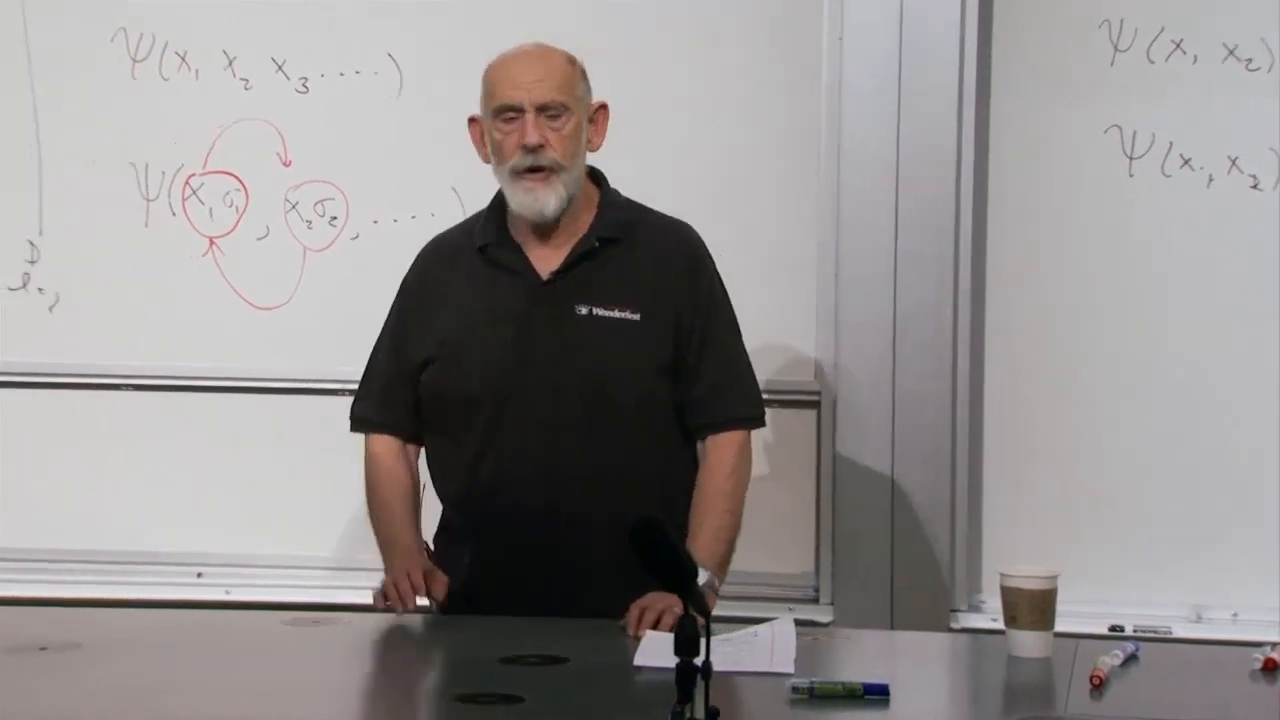
\includegraphics[width=0.9\linewidth]{lecture_05_frame_03.png}
\caption{Trao đổi hai hạt đồng nhất làm hoán đổi các nhãn vị trí--spin đầy đủ của chúng. Trạng thái boson không đổi, còn trạng thái fermion đổi dấu.}
\lectureframe{00:35:25}
\end{figure}

Đây là hai cách dùng tính tuyến tính khác nhau. Với một hạt,
\begin{equation}
\alpha\psi_0(x)+\beta\psi_1(x)
\end{equation}
là trạng thái chồng chập của hai khả năng. Với hai hạt,
\begin{equation}
\psi_0(x_1)\psi_1(x_2)
\end{equation}
là một biên độ tích trong không gian có hai tọa độ hạt. Phép đối xứng hóa hoặc phản đối xứng hóa kết hợp tích ấy với tích tương ứng sau khi trao đổi.

\begin{classroomqa}
\lecturetimestamp{00:36:13}
\audiencequestion{Trao đổi các hạt có tạo ra hiệu ứng giao thoa không?}
\lecturerresponse{Có. Biên độ fermion cùng trạng thái bằng không có thể được hiểu là giao thoa triệt tiêu giữa hai đóng góp sau khi trao đổi.}
\end{classroomqa}

\begin{classroomqa}
\lecturetimestamp{00:37:13}
\audiencequestion{Pauli có suy ra nguyên lý loại trừ bằng chính lập luận đối xứng này không?}
\lecturerresponse{Pauli bắt đầu từ một sự kiện thực nghiệm và tìm ra khuôn khổ toán học để diễn đạt nó. Ban đầu, ông không suy ra nguyên lý loại trừ từ một lý thuyết nền tảng hơn.}
\end{classroomqa}

Tính phản đối xứng cung cấp khuôn khổ toán học để diễn đạt quy tắc loại trừ thực nghiệm.

\begin{classroomqa}
\lecturetimestamp{00:39:01}
\audiencequestion{Giao thoa do trao đổi hạt có liên hệ với giao thoa giữa các đường đi khả dĩ không?}
\lecturerresponse{Có. Trong một lịch sử, hai hạt đi qua mà không cắt nhau; trong lịch sử kia, chúng cắt nhau để đến các đích đã hoán đổi. Các biên độ cộng lại với boson và có thể triệt tiêu với fermion.}
\end{classroomqa}

Phép trao đổi tạo ra dấu trừ thứ nhất. Phép quay tạo ra dấu trừ thứ hai.

\section{Dấu trừ thứ hai: phép quay một góc \texorpdfstring{\(2\pi\)}{2 pi}}

Một vòng quay trọn vẹn có vẻ như chẳng làm gì. Mọi hướng hình học thông thường đều trở về vị trí ban đầu sau một góc \(2\pi\). Tuy nhiên, điều cần trở về như cũ là xác suất và giá trị kỳ vọng. Bản thân vectơ trạng thái có thể trở về cùng với một pha tổng thể, giống như trong phép trao đổi.

\begin{classroomqa}
\lecturetimestamp{00:42:12}
\audiencequestion{Phép quay được thực hiện quanh trục nào, và toán tử sinh là mômen động lượng quỹ đạo, spin hay cả hai?}
\lecturerresponse{Có thể chọn một trục bên ngoài; dưới đây ta chọn trục \(z\). Toán tử sinh là mômen động lượng toàn phần, bao gồm cả phần quỹ đạo lẫn phần spin. Bản thân spin không nhất thiết phải hướng dọc theo trục đã chọn.}
\end{classroomqa}

\editorialnote{Các công thức mômen động lượng trong phần thảo luận này dùng đơn vị \(\hbar=1\), vì thế \(m\) là trị riêng không thứ nguyên của \(J_z\).}

Gọi \(\psi(\theta)\) là trạng thái thu được khi tham số quay tăng dần qua một góc \(\theta\). Theo quy ước dùng ở đây,
\begin{equation}
J_z\psi(\theta)
=
-i\frac{\partial}{\partial\theta}\psi(\theta).
\end{equation}
Với trạng thái có \(J_z\) xác định,
\begin{equation}
J_z\psi(\theta)=m\psi(\theta).
\end{equation}
Kết hợp các phương trình ta được
\begin{equation}
-i\frac{\partial}{\partial\theta}\psi(\theta)
=
m\psi(\theta),
\end{equation}
nghiệm là
\begin{equation}
\psi(\theta)=e^{im\theta}\psi(0).
\end{equation}

Các giá trị được phép của \(m\) là số nguyên hoặc bán nguyên. Do đó,
\begin{equation}
\psi(2\pi)
=
\begin{cases}
+\psi(0), & m\in\mathbb Z,\\[4pt]
-\psi(0), & m\in\mathbb Z+\tfrac12.
\end{cases}
\end{equation}
Sau thêm một vòng quay trọn vẹn,
\begin{equation}
\psi(4\pi)=\psi(0)
\end{equation}
trong cả hai trường hợp. Đây là dấu trừ thứ hai: trạng thái thuộc một đa tuyến mômen động lượng bán nguyên đổi dấu dưới phép quay góc \(2\pi\).

Dấu này không làm thay đổi \(\lvert\psi\rvert^2\), nên không thể quan sát được khi nó nhân với toàn bộ trạng thái. Dù vậy, phép quay góc \(2\pi\) không được biểu diễn bằng toán tử đơn vị trên trạng thái spin bán nguyên. Khác biệt này trở nên quan sát được khi dấu ấy tương đối với một biên độ kết hợp khác.

\section{Các đường đi quay góc \texorpdfstring{\(2\pi\) và \(4\pi\)}{2 pi và 4 pi}}

Có thể làm lộ rõ khác biệt giữa \(2\pi\) và \(4\pi\) mà không cần thêm đại số. Cầm một chiếc cốc bằng một tay rồi xoay trọn một vòng mà không buông tay. Cốc trở lại hướng ban đầu, nhưng cánh tay bị xoắn. Xoay tiếp thêm một vòng nữa thì có thể đưa cánh tay về vị trí ban đầu mà không phải đảo ngược chuyển động của cốc.

Một cách dựng liên quan là đặt một quả cầu trong hộp rồi nối nó với hộp bằng các sợi dây. Xoay quả cầu một góc \(2\pi\) sẽ làm dây rối. Trong không gian ba chiều thông thường, có thể gỡ rối dây ứng với một vòng quay \(4\pi\). Đối tượng cần xét không chỉ là hướng cuối cùng của quả cầu mà còn là đường đi qua không gian các phép quay.

\begin{classroomqa}
\lecturetimestamp{00:54:22}
\audiencequestion{Nếu xoay quả cầu hai vòng quanh cùng một trục thì có thể gỡ rối dây thật không? Việc đó có cần thêm một chiều không gian không?}
\lecturerresponse{Có thể gỡ rối đường đi \(4\pi\) trong không gian ba chiều thông thường. Thời gian tham số hóa chuyển động; nó không phải là một hướng không gian khác. Không thể gỡ rối đường đi \(2\pi\) theo cách này, trong khi có thể gỡ rối đường đi \(4\pi\).}
\end{classroomqa}

Các minh họa phân biệt đường đi \(2\pi\) không tầm thường với đường đi \(4\pi\) có thể gỡ rối, mà không triển khai lý thuyết hình thức về nhóm quay.

\section{Trao đổi và phép quay trong hình ảnh dây đai}

Giờ hai dấu trừ được đặt cạnh nhau. Trao đổi hai fermion đồng nhất làm đổi dấu hàm sóng chung của chúng. Quay một trạng thái spin bán nguyên một góc \(2\pi\) cũng làm đổi dấu trạng thái. Dây đai cho thấy mối liên hệ hình học giữa hai phép biến đổi.

Sắp xếp dây đai sao cho hai đầu dưới của nó đã bị hoán đổi. Nhìn theo cách khác, chính dây đai ấy có một vòng xoắn \(2\pi\). Thực hiện phép trao đổi cùng với phép quay \(2\pi\) sẽ xóa vòng xoắn và để lại dây đai không xoắn. Có thể liên tục biến quá trình kết hợp này về trạng thái không làm gì.\footnote{Trong bài giảng, nhận xét về phép trao đổi--quay được quy cho David Finkelstein. Tư liệu nguồn không nêu ấn phẩm cụ thể nào, nên ở đây tên ông chỉ được giữ lại như một sự quy thuộc.}

\begin{classroomqa}
\lecturetimestamp{01:01:12}
\audiencequestion{Đây chỉ là mệnh đề về cách dây đai nằm trong không gian, chứ không phải mệnh đề về tô pô của hạt, phải không?}
\lecturerresponse{Có thể xem dây đai như lịch sử của hạt trong không thời gian. Khi thời gian tăng theo chiều hướng lên, mặt cắt ngang của nó cho ta các vật thể kiểu hạt. Một cặp được tạo ra, một vật thể quay góc \(2\pi\), rồi hai vật thể đồng nhất được trao đổi. Trong lịch sử đó, các pha do phép quay và phép trao đổi triệt tiêu nhau.}
\end{classroomqa}

Lịch sử này làm rõ việc theo dõi pha. Bắt đầu khi chưa có hạt nào. Tại hai vị trí cách xa nhau, tạo ra một cặp hạt--phản hạt, để lại bốn hạt ở một thời điểm trung gian. Quay một hạt góc \(2\pi\) đồng thời trao đổi hai hạt đồng nhất khác trong cấu hình. Có thể biến dạng toàn bộ lịch sử này thành lịch sử sơ cấp, trong đó một cặp được tạo ra rồi sau đó hủy. Theo cách theo dõi dấu đang bàn đến, lịch sử tầm thường ấy không có pha bổ sung. Nếu \(\eta_{\mathrm{rot}}\) và \(\eta_{\mathrm{ex}}\) lần lượt là hai dấu, sự triệt tiêu được nêu bằng lời có thể viết gọn thành\footnote{Phương trình pha này ghi lại sự triệt tiêu được mô tả từ 01:06:50 đến 01:07:18; bài giảng trình bày phép dựng này như một gợi ý, chứ không phải một chứng minh nghiêm ngặt.}
\begin{equation}
\eta_{\mathrm{rot}}\eta_{\mathrm{ex}}=1.
\end{equation}

\begin{classroomqa}
\lecturetimestamp{01:03:34}
\audiencequestion{Có thể liên hệ phép trao đổi với phép quay bằng cách cho mỗi hạt trong hai hạt chuyển động một góc \(\pi\) rồi định hướng lại chúng không?}
\lecturerresponse{Cách dựng đó có thể phản ánh toán học liên quan, nhưng nó dùng hai phép quay riêng biệt, mỗi phép một góc \(\pi\). Quá trình đang phân tích ở đây chỉ có một phép quay góc \(2\pi\), nên hai lập luận không đồng nhất.}
\end{classroomqa}

Lập luận này dựa vào khả năng tạo ra và hủy các vật thể kiểu hạt. Nó sẽ không có dạng này trong một lý thuyết mà các hạt tồn tại vĩnh viễn. Lập luận cũng không được đưa ra như chứng minh chuẩn của định lý spin--thống kê. Mục đích của nó là chỉ ra một lý do tô pô khiến các dấu do trao đổi và phép quay tương thích với nhau.

\section{Các cấu hình cục bộ, ảnh gương và sự hủy}

Có thể lặp lại phép dựng này với các cấu hình trường định xứ. Giả sử một hay nhiều trường nhận giá trị chân không ở hầu hết mọi nơi, nhưng có hình dạng và cấu trúc khác không trong một vùng nhỏ. Cấu hình định xứ ấy là một cấu hình dạng cục.

Giờ tạo cấu hình thứ hai là ảnh gương thích hợp của cấu hình thứ nhất. Gọi một cấu hình là hạt và cấu hình kia là phản hạt. Đưa chúng lại gần nhau. Các phần tương ứng của hai cấu hình trường gặp nhau và triệt tiêu lẫn nhau. Ở một giai đoạn trung gian, một số phần của các cấu hình dạng cục có thể đã biến mất trong khi những phần khác vẫn còn. Tiếp tục biến dạng sẽ xóa cấu trúc còn lại và đưa các trường trở về cấu hình chân không. Hai vòng xoắn ngược chiều trong dây đai cho ta cùng hình ảnh: đẩy chúng lại gần nhau, chúng sẽ tháo xoắn.

Có thể chạy quá trình này theo chiều ngược lại. Không gian trống có thể sinh ra một cấu hình dạng cục cùng ảnh gương của nó. Ta có thể tạo hai cặp như vậy, quay một cấu hình dạng cục một góc \(2\pi\), trao đổi hai cấu hình dạng cục đồng nhất rồi lại hủy các cặp. Khi đó, sự triệt tiêu giữa phép trao đổi--quay vẫn áp dụng. Đây vẫn là phần mở rộng mang tính trực giác của phép dựng, chứ không phải định lý về mọi kích thích định xứ.

\begin{classroomqa}
\lecturetimestamp{01:11:30}
\audiencequestion{Có hiện thực vật lý nào của những cấu hình trường dạng cục này không?}
\lecturerresponse{Có. Ví dụ gồm hạt nhân trong mô tả kiểu Skyrmion, đơn cực từ và các kích thích trường khác có tính chất như hạt.}
\end{classroomqa}

Hình ảnh các cấu hình dạng cục cùng ảnh gương giúp ta hiểu được phép khái quát hóa. Điều quan trọng không phải là vật thể ban đầu có phải hạt điểm sơ cấp hay không, mà là một kích thích kiểu hạt và đối tác của nó có thể được tạo ra, đưa lại gần nhau rồi hủy một cách liên tục. Đặc điểm đó gợi mở một mối liên hệ rộng hơn giữa phép quay và hành vi trao đổi.

\begin{classroomqa}
\lecturetimestamp{01:16:12}
\audiencequestion{Spin bằng một phần hai có nghĩa là trạng thái chỉ tích lũy một nửa pha quay thông thường phải không?}
\lecturerresponse{Pha theo quy ước này là \(e^{im\theta}\). Với \(m\) bán nguyên, phép quay góc \(2\pi\) cho \(-1\), còn phép quay góc \(4\pi\) cho \(+1\).}
\end{classroomqa}

\section{Dấu tổng thể và thí nghiệm cho kết quả không}

Có thể quan sát dấu trừ do phép quay góc \(2\pi\) không? Trước hết, hãy xét một thí nghiệm mà trong đó không thể quan sát dấu ấy. Giam một electron trong từ trường, để spin của nó đi theo từ trường khi thiết bị được quay chậm một góc \(2\pi\), rồi thả electron vào một thiết bị giao thoa. So sánh với quy trình tương tự nhưng không có phép quay.

Phép quay làm trạng thái biến đổi theo
\begin{equation}
\psi\longmapsto-\psi,
\end{equation}
nhưng dấu trừ nhân với toàn bộ trạng thái. Mọi xác suất đều không đổi, nên mẫu giao thoa cuối cùng không lưu lại dấu vết nào cho biết phép quay sơ bộ có diễn ra hay không. Đây là một thí nghiệm cho kết quả không: pha chung không có gì để giao thoa với nó.

\begin{classroomqa}
\lecturetimestamp{01:20:01}
\audiencequestion{Tại sao phải quay từ trường thật chậm?}
\lecturerresponse{Spin phải tiếp tục đi theo từ trường đang quay. Nếu kéo từ trường quay quá nhanh, spin sẽ không còn duy trì được sự khóa hướng theo nó.}
\end{classroomqa}

\section{Một electron trong hai nhánh kết hợp}

Dấu này trở nên quan sát được khi xét tương đối. Cho một electron đi qua bộ tách chùm. Một phần hàm sóng đi theo đường này, phần còn lại đi theo đường kia:
\begin{equation}
\psi(x)=\psi_1(x)+\psi_2(x).
\end{equation}
Đây là một electron, không phải hai electron. Nó ở trạng thái chồng chập kết hợp của hai khả năng. Cần phân biệt rõ: hai bó sóng không phải là hai hạt độc lập.

Dẫn hai bó sóng vào những vùng riêng biệt có chứa từ trường. Quay từ trường ở một vùng góc \(2\pi\), còn vùng kia giữ nguyên. Với trạng thái spin bán nguyên,
\begin{equation}
\psi_1(x)+\psi_2(x)
\longmapsto
\psi_1(x)-\psi_2(x),
\end{equation}
trong đó nhánh bị quay được gán nhãn \(2\). Giờ dấu này là tương đối. Khi hai bó sóng chồng lấp trở lại, phép cộng trở thành phép trừ. Một điểm giao thoa tăng cường có thể trở thành điểm giao thoa triệt tiêu, thậm chí là một nút.

\begin{classroomqa}
\lecturetimestamp{01:23:46}
\audiencequestion{Nếu chỉ có một electron nhưng hai nhánh hàm sóng, thì cái gì đang được quay?}
\lecturerresponse{Electron ở trạng thái chồng chập kết hợp của hai khả năng định xứ. Một nhánh được quay, nhánh kia thì không. Nếu mở các hộp để biết khả năng nào đã xảy ra, phép đo ấy sẽ phá hủy giao thoa.}
\end{classroomqa}

Mở các hộp ra chỉ cho biết electron duy nhất nằm trong hộp này hay hộp kia. Nếu không thực hiện phép đo đó, cả hai biên độ vẫn còn trong trạng thái. Lặp lại thí nghiệm sẽ tích lũy mẫu giao thoa, mỗi lần phát hiện một electron. Tại nút do dấu trừ tương đối tạo ra, không phát hiện được electron nào.

\section{Tiền động từ và giao thoa hai khe}

Một bố trí sơ đồ thực tế hơn thay cho thí nghiệm với chiếc hộp cần thời gian rất lâu. Tách một sóng electron kết hợp thành hai đường đi. Trên một đường, cho electron đi qua vùng từ trường khi spin ban đầu vuông góc với từ trường. Khi đó spin tiến động. Bằng cách chọn cường độ từ trường và thời gian bay, có thể làm spin ở nhánh đó quay trọn một vòng \(2\pi\), trong khi nhánh kia không trải qua phép quay như vậy.\footnote{Bài giảng nói rằng một thí nghiệm liên quan đến pha spinor đã được thực hiện và mô tả nguyên lý của thí nghiệm, nhưng tư liệu nguồn không xác định bài báo hay thiết bị cụ thể. Vì vậy, phần trình bày ở đây chỉ giới hạn ở phép dựng được nêu trong bài giảng.}

\begin{classroomqa}
\lecturetimestamp{01:27:05}
\audiencequestion{Làm sao xác định được đường đi của electron đơn lẻ?}
\lecturerresponse{Không thể xác định mà không làm hỏng thí nghiệm. Bất kỳ phép đo nào ghi lại đường đi của electron đều phá hủy giao thoa.}
\end{classroomqa}

\begin{classroomqa}
\lecturetimestamp{01:27:50}
\audiencequestion{Chính xác thì một nhánh của hàm sóng là gì, và bộ tách chùm tạo ra hai nhánh bằng cách nào?}
\lecturerresponse{Nhánh là một bó sóng định xứ dọc theo một đường đi. Bộ tách biến sóng tới thành hai bó sóng tách biệt trong không gian; các trường điện hoặc từ có thể dẫn chúng theo những đường khác nhau.}
\end{classroomqa}

Ngoài vùng từ trường, đây là thí nghiệm hai khe. Sóng electron tới tách thành hai bó sóng. Các sóng đi ra lan rộng vào một vùng phát hiện chung, nơi các biên độ chồng lấp. Nếu không có phép quay tương đối, các biên độ ở tâm có thể cộng lại. Phép quay spin góc \(2\pi\) trên một đường đi đảo dấu một biên độ và có thể làm các đóng góp tương ứng triệt tiêu nhau.

\begin{classroomqa}
\lecturetimestamp{01:30:46}
\audiencequestion{Nếu electron đi qua các ống hay khe riêng biệt, làm sao có thể xảy ra giao thoa?}
\lecturerresponse{Phép phát hiện cuối cùng không cho biết đường đi. Hai biên độ sóng đi ra lan rộng và chồng lấp tại đầu dò. Quan sát để biết hạt đã đi theo đường nào sẽ phá hủy giao thoa.}
\end{classroomqa}

\begin{classroomqa}
\lecturetimestamp{01:33:22}
\audiencequestion{Đường kính ống hay khe có phải xấp xỉ bước sóng electron không?}
\lecturerresponse{Với một cách hiện thực hóa thí nghiệm hai khe dựa đúng nghĩa vào nhiễu xạ, khe mở phải đủ nhỏ để tạo ra độ lan rộng cần thiết. Thiết bị đang mô tả chỉ mang tính sơ đồ, không phải một thiết kế thực dụng.}
\end{classroomqa}

\begin{classroomqa}
\lecturetimestamp{01:33:44}
\audiencequestion{Liệu phép quay phân cực của photon một góc tương ứng với \(2\pi\) có khiến hình giao thoa không thay đổi?}
\lecturerresponse{Có. Photon có spin nguyên, nên một phép quay trọn vẹn \(2\pi\) không tạo ra dấu trừ fermion.}
\end{classroomqa}

\begin{classroomqa}
\lecturetimestamp{01:34:12}
\audiencequestion{Thí nghiệm thực tế khác phiên bản lý tưởng hóa ở điểm nào?}
\lecturerresponse{Trong cách dựng lý tưởng, spin được quay đoạn nhiệt. Theo mô tả thực tế, electron chuyển động qua một vùng từ trường và spin của nó tiến động nhanh hơn, nhưng pha đo được vẫn là pha ứng với một vòng quay \(2\pi\).}
\end{classroomqa}

Cách dựng chậm làm nổi bật ý tưởng bằng cách bảo đảm spin đi theo từ trường mà không có chuyển động bổ sung. Cách dựa trên sự tiến động tạo ra cùng dấu tương đối nhờ động lực học. Dù dùng cách nào, hai đường đi phải không còn phân biệt được thì mới có thể xuất hiện hình giao thoa.

\begin{classroomqa}
\lecturetimestamp{01:36:15}
\audiencequestion{Sau bộ tách, có cần cho hai nhánh kết hợp lại không?}
\lecturerresponse{Có. Các gói sóng đi ra phải chồng lấp lên nhau hoặc trải rộng trên cùng một vùng ghi nhận, để biên độ của chúng có thể tạo thành hình giao thoa.}
\end{classroomqa}

\begin{classroomqa}
\lecturetimestamp{01:38:12}
\audiencequestion{Thí nghiệm quay một electron này có phải là hệ quả của nguyên lý loại trừ Pauli không?}
\lecturerresponse{Không. Ở đây chỉ có một electron. Thí nghiệm đo pha spinor khi quay, chứ không đo sự loại trừ hai fermion khỏi cùng một trạng thái.}
\end{classroomqa}

\section{Giao thoa do trao đổi và phép quay tương đối}

Có thể làm lộ dấu trao đổi bằng cùng một phương pháp tổng quát, dù thiết bị được đề xuất phức tạp hơn. Bắt đầu với hai electron và tách hàm sóng chung của chúng thành hai nhánh kết hợp. Vẫn chỉ có hai electron, chứ không phải bốn: cặp electron đi theo một phương án hoặc phương án kia. Ở một nhánh, hoán đổi hai electron; ở nhánh còn lại, giữ nguyên thứ tự của chúng. Sau khi hai nhánh được đưa lại với nhau, dấu trao đổi fermion xuất hiện dưới dạng pha tương đối và có thể làm thay đổi giao thoa.

Đề xuất cuối cùng so sánh trực tiếp hai dấu trừ. Một nhánh nhận pha trao đổi fermion, còn nhánh kia nhận pha tương ứng với phép quay \(2\pi\). Cả hai pha đều bằng \(-1\), nên hiệu ứng tương đối triệt tiêu.\footnote{Bản ghi trong khoảng từ 01:40:26 đến 01:41:15 cho thấy rõ pha trao đổi, pha của phép quay \(2\pi\) và sự triệt tiêu của chúng, nhưng không thể xác định từ phần lời nói hiện có phép quay được gán cụ thể như thế nào.} Bài giảng trình bày đây là một thí nghiệm tư tưởng được đề xuất và cho biết, theo hiểu biết của người nói, thí nghiệm này chưa từng được thực hiện.

\begin{classroomqa}
\lecturetimestamp{01:41:34}
\audiencequestion{Việc quan sát thấy pha trao đổi có thách thức tính không thể phân biệt của hai electron không?}
\lecturerresponse{Không. Tính không thể phân biệt trong cơ học lượng tử tinh tế hơn sự đồng nhất theo nghĩa cổ điển. Nó cho phép vectơ trạng thái đổi dấu khi trao đổi, dù không có nhãn quan sát được nào phân biệt các hạt.}
\end{classroomqa}

Còn một điểm cần lưu ý cuối cùng. Quay toàn bộ một thế giới cô lập qua \(2\pi\) chỉ tạo ra một pha chung, và không thí nghiệm nội tại nào có thể phát hiện được pha đó. Thí nghiệm có thể phát hiện được là phép quay một nhánh kết hợp tương đối với nhánh kia. Vì vậy, điều được quan sát không phải là một dấu tuyệt đối, mà là giao thoa do một dấu tương đối tạo ra.

\chapter{Dao động tử, số chiếm và trường lượng tử đầu tiên}

Lý thuyết trường lượng tử là khuôn khổ của chúng ta để mô tả hầu như toàn bộ vật lý phi hấp dẫn đã biết. Không nên nhầm khẳng định đó với việc cho rằng có thể giải mọi bài toán. Nguyên tử hydro còn xử lý được; đến một nguyên tử như bo, phép tính đã khó hơn nhiều, còn một con người thì vượt xa mọi phép tính lý thuyết trường khả thi. Khuôn khổ này có thể là nền tảng, nhưng các phương trình của nó vẫn cực kỳ khó giải.

Vì vậy, ta sẽ bắt đầu theo cách sơ cấp nhất có thể. Chủ đề này đôi khi được gọi là \emph{lượng tử hóa lần thứ hai}, nhưng tên gọi ấy sẽ chưa có nhiều ý nghĩa cho đến khi ta xây dựng xong bộ công cụ cần thiết. Con đường ngắn nhất không bắt đầu từ một trường tương đối tính, mà từ dao động tử điều hòa. Lò xo không phải là điều cốt yếu. Điều quan trọng là đại số của các toán tử nâng và hạ. Khi lặp lại đại số ấy cho nhiều mode, toán tử nâng sẽ không còn chỉ có nghĩa là ``nâng dao động tử lên một mức'' mà sẽ thực sự có nghĩa là ``tạo ra một hạt.''

\section{Dao động tử dưới góc nhìn đại số}

Với một dao động tử, ký hiệu \(a^\dagger\) là toán tử nâng kích thích, còn \(a\) là toán tử hạ kích thích. Các ký hiệu \(a_+\) và \(a_-\) cũng tương đương, nhưng ký hiệu dấu dagger báo trước cách viết dùng trong lý thuyết trường. Trạng thái đáy thỏa mãn
\begin{equation}
a|0\rangle=0,
\end{equation}
và toán tử số là
\begin{equation}
N=a^\dagger a,
\qquad
N|n\rangle=n|n\rangle.
\end{equation}
Hai toán tử bậc thang là liên hợp Hermite của nhau, và hệ thức giao hoán cốt yếu của chúng là
\begin{equation}
[a,a^\dagger]=1.
\label{eq:l06-single-commutator}
\end{equation}
Đại số nhỏ bé này gần như đã bao quát toàn bộ dao động tử.

Có thể biểu diễn \(a\) và \(a^\dagger\) bằng các tổ hợp tuyến tính thích hợp của vị trí và động lượng. Quy ước cụ thể phụ thuộc vào cách chuẩn hóa \(x\), \(p\), \(m\) và \(\omega\); phát biểu bất biến hữu ích ở đây là \(a^\dagger a\) dựng lại Hamilton của dao động tử bậc hai, ngoại trừ năng lượng điểm không cộng thêm. Do đó
\begin{equation}
H=\hbar\omega\left(N+\frac12\right).
\end{equation}
Trong phần thảo luận này, ta bỏ số hạng hằng và xét
\begin{equation}
H=\hbar\omega N.
\label{eq:l06-one-oscillator-hamiltonian}
\end{equation}
Tần số cho biết cái giá của một kích thích. Nâng \(n\) thêm một mức tốn \(\hbar\omega\); hạ \(n\) một mức giải phóng đúng chừng ấy năng lượng.

\section{Nhiều dao động tử độc lập}

Bây giờ xét nhiều dao động tử và đánh nhãn chúng bằng \(i\). Nhãn này chỉ là một chỉ số, không phải đơn vị ảo. Có thể có hữu hạn hoặc vô hạn mode. Một tập hợp các lò xo độc lập là một hình dung; các mode riêng của dây đàn vĩ cầm lý tưởng là một hình dung khác. Trong các ứng dụng lý thuyết trường, trường hợp có vô hạn mode mới là trường hợp quan trọng.

Tính độc lập có ý nghĩa về mặt toán tử. Các toán tử thuộc về những hệ con thực sự độc lập thì giao hoán với nhau. Nếu không, các đại lượng tương ứng không thể được đo độc lập, và ngay từ đầu các hệ ấy đã không độc lập. Vì vậy, ta có
\begin{align}
[a_i,a_j]&=0, \\
[a_i^\dagger,a_j^\dagger]&=0, \\
[a_i,a_j^\dagger]&=\delta_{ij}.
\label{eq:l06-many-commutators}
\end{align}
Khi \(i\ne j\), mọi thứ thuộc về hai mode đều giao hoán. Khi \(i=j\), dòng cuối rút gọn thành Phương trình~\eqref{eq:l06-single-commutator}.

Mỗi dao động tử có toán tử số riêng và, nói chung, tần số riêng:
\begin{equation}
N_i=a_i^\dagger a_i,
\qquad
H=\sum_i\hbar\omega_i N_i.
\label{eq:l06-many-hamiltonian}
\end{equation}
Một trạng thái riêng đồng thời được đánh nhãn bằng danh sách đầy đủ
\begin{equation}
|n_1,n_2,n_3,\ldots\rangle,
\qquad n_i=0,1,2,\ldots.
\label{eq:l06-occupation-ket}
\end{equation}
Số nguyên \(n_i\) được gọi là \emph{số chiếm} của dao động tử thứ \(i\). Ở giai đoạn này, đó chỉ là thuật ngữ. Chẳng bao lâu nữa, nó sẽ đếm số hạt chiếm một trạng thái một hạt, và tên gọi ấy sẽ đúng theo nghĩa đen.

Trạng thái có mọi số chiếm bằng không là
\begin{equation}
|0\rangle\equiv|0,0,0,\ldots\rangle,
\qquad a_i|0\rangle=0\quad\text{for every }i.
\label{eq:l06-oscillator-vacuum}
\end{equation}

\begin{classroomqa}\lecturetimestamp{00:15:27}\audiencequestion{Một họ dao động tử vô hạn có tương ứng với liên tục các mode của một hệ như dây đàn vĩ cầm không?}\lecturerresponse{Có, đối với dây lý tưởng. Dây thực được cấu tạo từ các nguyên tử, nên các bước sóng đủ ngắn cuối cùng sẽ gặp một ngưỡng cắt vi mô. Dù vậy, mô hình liên tục vẫn gợi ý cho ta tập hợp vô hạn mode được dùng trong lý thuyết trường.}\end{classroomqa}

\section{Vì sao các hệ số bậc thang là căn bậc hai}

Tác dụng của \(a^\dagger\) phải nâng trạng thái riêng của \(N\) lên trạng thái riêng kế tiếp, nhưng điều kiện chuẩn hóa vẫn cho phép có một hệ số:
\begin{equation}
a^\dagger|n\rangle=c_n|n+1\rangle.
\label{eq:l06-unknown-coefficient}
\end{equation}

\begin{figure}[htbp]\centering
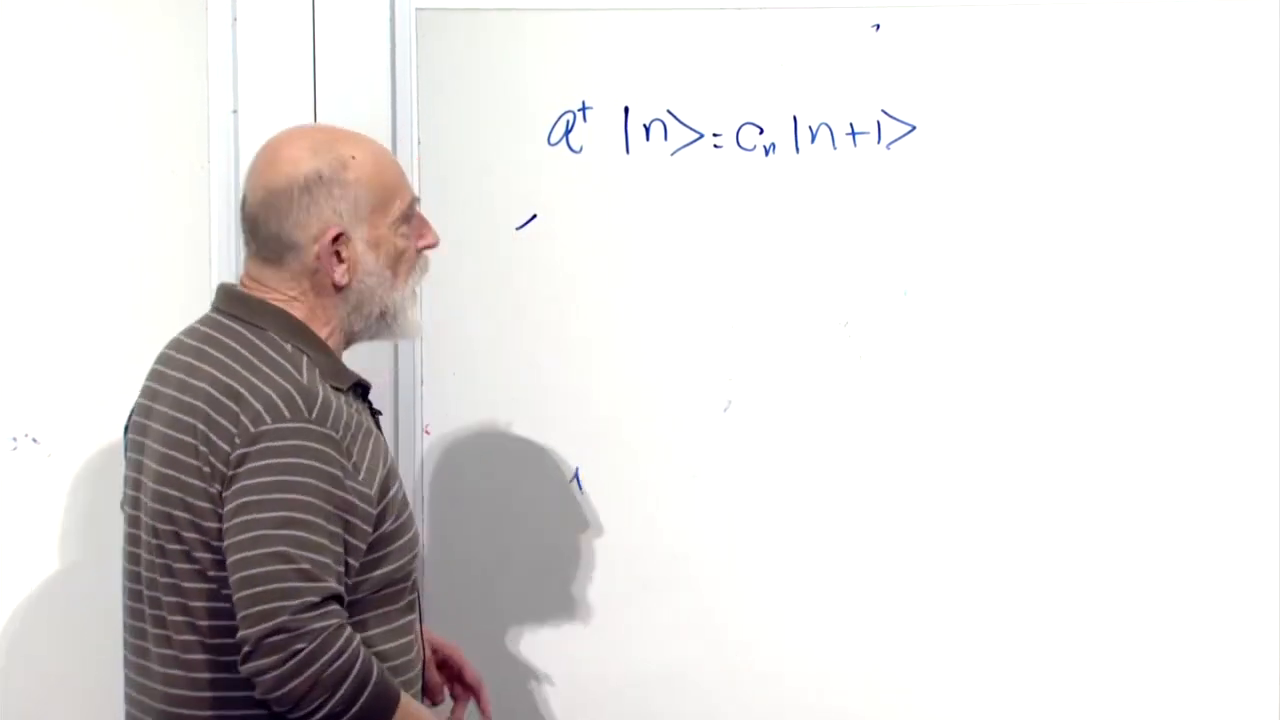
\includegraphics[width=0.9\linewidth]{lecture_06_frame_01.png}\caption{Hệ số bậc thang được đưa vào trước khi suy ra cách chuẩn hóa của nó. Phương trình trên bảng được chép lại trong Phương trình~\eqref{eq:l06-unknown-coefficient}}\lectureframe{00:19:38}\end{figure}

Chọn quy ước pha sao cho \(c_n\) là số thực. Lấy liên hợp Hermite, ta được
\begin{equation}
\langle n|a=c_n\langle n+1|.
\end{equation}
Nhân hai hệ thức với nhau và dùng các trạng thái cơ sở đã chuẩn hóa,
\begin{align}
c_n^2
&=\langle n|aa^\dagger|n\rangle \\
&=\langle n|(a^\dagger a+1)|n\rangle \\
&=\langle n|(N+1)|n\rangle \\
&=n+1.
\end{align}
Suy ra
\begin{equation}
a^\dagger|n\rangle=\sqrt{n+1}\,|n+1\rangle.
\label{eq:l06-raising-rule}
\end{equation}

\begin{classroomqa}\lecturetimestamp{00:22:35}\audiencequestion{Vì sao có thể đặt \(\langle n+1|n+1\rangle=1\) trước khi tìm \(c_n\)}\lecturerresponse{Ngay từ đầu, các vectơ riêng được chọn làm một cơ sở đã chuẩn hóa. Điều kiện chuẩn hóa của chúng không xác định chuẩn hóa của \(a^\dagger|n\rangle\); thông tin còn thiếu ấy chính là hệ số \(c_n\)}\end{classroomqa}

Quy tắc hạ được suy ra tương tự:
\begin{equation}
a|n\rangle=\sqrt n\,|n-1\rangle.
\label{eq:l06-lowering-rule}
\end{equation}
Khi \(n=0\), hệ số tự động triệt tiêu, nên quy tắc này bao gồm cả trường hợp \(a|0\rangle=0\). Với nhiều mode, toán tử chỉ thay đổi số chiếm ở vị trí tương ứng với chính nó:
\begin{align}
a_i^\dagger|n_1,\ldots,n_i,\ldots\rangle
&=\sqrt{n_i+1}\,|n_1,\ldots,n_i+1,\ldots\rangle, \\
a_i|n_1,\ldots,n_i,\ldots\rangle
&=\sqrt{n_i}\,|n_1,\ldots,n_i-1,\ldots\rangle.
\label{eq:l06-multimode-ladders}
\end{align}
Các số chiếm khác không thay đổi.

\section{Hàm sóng không phải là trường lượng tử}

Trước khi định nghĩa trường, ta cần phân biệt nó với hàm sóng quen thuộc. Ba điểm tương phản sẽ dẫn dắt bước chuyển này.

Thứ nhất, hàm sóng của một hạt
\begin{equation}
\psi(x)=\langle x|\psi\rangle
\end{equation}
là một biểu diễn của vectơ trạng thái. Bản thân nó không phải là một đại lượng có thể quan sát. Ta đo vị trí, động lượng, mômen động lượng và các toán tử khác; hàm sóng cung cấp các biên độ dùng để tính xác suất nhận được những kết quả ấy.

Thứ hai, hàm sóng của nhiều hạt phụ thuộc vào vị trí của tất cả các hạt. Với hai hạt có các vectơ vị trí tạm gọi là \(x\) và \(y\),
\begin{equation}
\psi(x,y)=\langle x,y|\psi\rangle.
\end{equation}
Ở đây, \(x\) và \(y\) lần lượt chỉ hai hạt khác nhau; chúng không phải là các thành phần Cartesian thứ \(x\) và thứ \(y\) của cùng một vectơ vị trí. Với \(N\) hạt, trạng thái được biểu diễn bằng
\begin{equation}
\psi(x_1,x_2,\ldots,x_N).
\end{equation}

Thứ ba, hàm sóng này mô tả một số hạt cố định. Hàm sóng của mười lăm hạt có mười lăm đối số vị trí và thuộc về không gian Hilbert của mười lăm hạt. Tự nó, hàm sóng ấy không mô tả một quá trình trong đó số hạt thay đổi từ mười lăm thành mười bốn hoặc mười sáu.

Trường lượng tử đảo ngược những đặc điểm này. Nó là một toán tử chứ không phải một trạng thái, phụ thuộc vào một điểm không gian \(x\), và tác dụng lên một không gian trạng thái chứa mọi sector số hạt. Cụm từ ``một điểm'' có nghĩa là một vectơ vị trí biến thiên tự do. Không có nghĩa là \(x\) đã được gán một giá trị số cụ thể.

Có một điều cần lưu ý, sau này sẽ quan trọng. Trường \(\Psi(x)\) được giới thiệu dưới đây không Hermite, nên theo nghĩa nghiêm ngặt, bản thân nó không phải là đại lượng có thể quan sát. Các tổ hợp Hermite của nó mới là đại lượng có thể quan sát. Vì vậy, phát biểu tạm thời rằng trường có thể đo được được làm chính xác hơn chứ không bị bác bỏ: trường là các hàm nhận giá trị toán tử, còn các tổ hợp Hermite của chúng biểu diễn những đại lượng có thể đo.

\begin{classroomqa}\lecturetimestamp{00:36:52}\audiencequestion{Nếu trường là hàm của một vị trí, vị trí đó có thể biến thiên không? Và \(y\) trong hàm sóng hai hạt đã đi đâu?}\lecturerresponse{Điểm \(x\) biến thiên trên khắp không gian. ``Một vị trí'' có nghĩa là toán tử có một đối số không gian, chứ không phải đối số ấy cố định. Trong \(\psi(x,y)\), các ký hiệu \(x\) và \(y\) chỉ vị trí của hai hạt; tương đương, chúng là \(x_1\) và \(x_2\). Chúng không phải là hai thành phần Cartesian của đối số trường.}\end{classroomqa}

\begin{classroomqa}\lecturetimestamp{00:38:15}\audiencequestion{Hàm sóng của số hạt cố định và cách mô tả bằng trường liên hệ với nhau thế nào, và chúng có mô tả những loại hạt khác nhau không?}\lecturerresponse{Mối liên hệ ấy là cấu trúc cốt lõi sẽ được xây dựng tiếp theo. Các hạt là cùng một loại. Trong bài giảng này, chúng là boson; fermion đòi hỏi một đại số khác.}\end{classroomqa}

\section{Một hạt trong hộp}

Tạm thời quay lại cơ học lượng tử thông thường của một hạt. Đặt một hạt vào hộp một chiều. Khi chỉ có một hạt, sự phân biệt giữa boson và fermion không liên quan: không có hạt giống hệt thứ hai để xét phép hoán đổi hoặc nguyên lý loại trừ.

Gọi
\begin{equation}
\psi_1(x),\ \psi_2(x),\ \psi_3(x),\ldots
\end{equation}
là các hàm riêng năng lượng. Mode thấp nhất là sóng trơn nhất triệt tiêu ở hai vách. Mode kế tiếp có một nút bên trong, còn các mode năng lượng cao hơn dao động nhanh hơn. Trong giếng vuông vô hạn lý tưởng có chiều rộng \(L\), một cơ sở trực chuẩn đã chuẩn hóa thuận tiện là
\begin{equation}
\psi_i(x)=\sqrt{\frac{2}{L}}\sin\!\left(\frac{i\pi x}{L}\right),
\qquad 0<x<L.
\label{eq:l06-box-basis}
\end{equation}
Công thức sin tường minh là một ví dụ chuẩn cho hình phác họa định tính trên bảng; lập luận dưới đây chỉ cần một tập đầy đủ các trạng thái một hạt trực chuẩn.

\begin{figure}[htbp]\centering
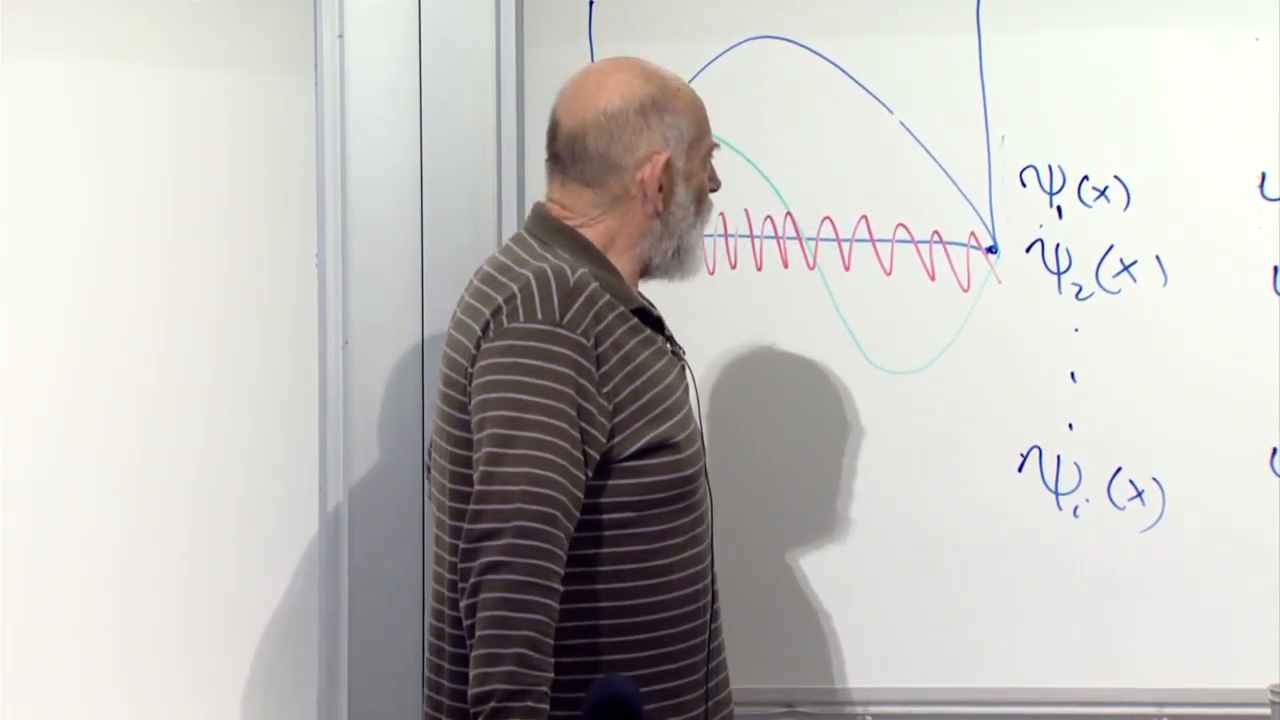
\includegraphics[width=0.9\linewidth]{lecture_06_frame_03.png}\caption{Các mode của hạt trong hộp, sắp theo năng lượng tăng dần. Mode đầu tiên không có nút bên trong, mode thứ hai có một nút, còn các mode bậc cao bị lược đi dao động ngày càng nhanh.}\lectureframe{00:43:10}\end{figure}

Có thể vẽ lại cấu trúc ấy mà không bị hình ảnh trên bảng trực tiếp che khuất:
\begin{figure}[htbp]\centering
\begin{tikzpicture}[x=1cm,y=1cm]
  \draw[thick] (0,0) -- (0,3.8);
  \draw[thick] (7,0) -- (7,3.8);
  \draw[gray!55] (0,2.75) -- (7,2.75);
  \draw[gray!55] (0,1.35) -- (7,1.35);
  \draw[blue!75!black,thick,domain=0:7,samples=120]
    plot (\x,{2.75+0.62*sin(180*\x/7)});
  \draw[teal!70!black,thick,domain=0:7,samples=120]
    plot (\x,{1.35+0.55*sin(360*\x/7)});
  \node[right] at (7.15,3.15) {$\psi_1(x)$};
  \node[right] at (7.15,1.70) {$\psi_2(x)$};
  \node at (3.5,0.45) {$\vdots\quad \psi_i(x)$};
\end{tikzpicture}\caption{Bản dựng lại rõ ràng của hình phác họa định tính các mode trong hộp. Độ dịch theo phương đứng giúp tách các hàm riêng cho dễ nhìn, không phải là một tọa độ vật lý bổ sung.}\end{figure}

Chỉ số \(i\) đánh nhãn một trạng thái một hạt, không phải một hạt và cũng không phải số nút. Với cơ sở trong hộp, \(i\) tình cờ bằng số nút bên trong cộng một. Mỗi trạng thái có năng lượng \(\varepsilon_i\). Theo ký hiệu của bài giảng, ta có thể viết năng lượng này là \(\hbar\omega_i\), hoặc đơn giản là \(\omega_i\) sau khi đặt \(\hbar=1\).

\begin{classroomqa}\lecturetimestamp{00:39:01}\audiencequestion{Giả thiết về tính độc lập trước đó có chính xác không, và chỉ số \(i\) có thể đánh nhãn các trạng thái khả dĩ của electron trong nguyên tử không?}\lecturerresponse{Trong cấu trúc các mode độc lập, các hệ thức giao hoán giữa những mode khác nhau là chính xác. Chỉ số này có thể đánh nhãn các trạng thái một hạt trong nguyên tử. Tuy nhiên, nếu các hạt tương tác thì Hamilton đơn giản của các mode độc lập không còn mô tả đầy đủ hệ nữa.}\end{classroomqa}

\begin{classroomqa}\lecturetimestamp{00:40:34}\audiencequestion{Hạt trong hộp có phải là boson không?}\lecturerresponse{Có thể là boson, nhưng với một hạt thì thống kê không quan trọng. Nguyên lý loại trừ và phép hoán đổi chỉ có ý nghĩa khi có nhiều hơn một hạt giống hệt nhau.}\end{classroomqa}

\section{Từ các mode trong hộp đến không gian Fock}

Bây giờ cho phép có số boson giống hệt nhau bất kỳ trong hộp. Một số \(n_1\) hạt có thể chiếm \(\psi_1\), một số \(n_2\) hạt có thể chiếm \(\psi_2\), vân vân. Vì thế, một trạng thái cơ sở có dạng
\begin{equation}
|n_1,n_2,n_3,\ldots\rangle.
\end{equation}
Đây chính xác là ký hiệu đã dùng cho nhiều dao động tử. Sự tương ứng mang tính cấu trúc: gán một dao động tử cho mỗi trạng thái một hạt, rồi đồng nhất số kích thích của dao động tử với số hạt chiếm trạng thái ấy.

Boson là điều thiết yếu ở đây vì mỗi \(n_i\) có thể là bất kỳ số nguyên không âm nào. Với fermion, mỗi trạng thái một hạt chỉ có thể để trống hoặc được chiếm bởi một hạt, tuyệt đối không thể bị chiếm bởi hai hạt; vì vậy không thể giữ nguyên đại số dao động tử thông thường.

Giờ đây, có thể định nghĩa các toán tử thông qua tác dụng của chúng lên cơ sở số chiếm. Toán tử \(a_i^\dagger\) tạo ra một hạt trong trạng thái một hạt \(i\); toán tử \(a_i\) loại bỏ một hạt:
\begin{align}
a_i^\dagger|n_1,\ldots,n_i,\ldots\rangle
&=\sqrt{n_i+1}\,|n_1,\ldots,n_i+1,\ldots\rangle, \\
a_i|n_1,\ldots,n_i,\ldots\rangle
&=\sqrt{n_i}\,|n_1,\ldots,n_i-1,\ldots\rangle.
\end{align}
Đây không phải là phép ví von được đưa ra sau đó. Đó là định nghĩa của các toán tử tạo và hủy boson trên cơ sở này. Vì cơ sở sinh ra toàn bộ không gian, định nghĩa này xác định tác dụng của chúng lên mọi trạng thái nhờ tính tuyến tính.

\begin{classroomqa}\lecturetimestamp{00:47:11}\audiencequestion{\(n_1,n_2,n_3\) có phải là các trạng thái lượng tử không?}\lecturerresponse{Các nhãn \(1,2,3,\ldots\) xác định các trạng thái một hạt. Các ký hiệu \(n_1,n_2,n_3,\ldots\) là số hạt chiếm những trạng thái ấy. Giữ phân biệt giữa nhãn trạng thái và số chiếm của nó là yêu cầu ký hiệu chính yếu.}\end{classroomqa}

\subsection{Ý nghĩa của căn bậc hai}

Thừa số \(\sqrt{n_i+1}\) không biểu thị một hạt bổ sung hay một quá trình vật lý riêng biệt. Nó giúp toán tử có chuẩn hóa và đại số chính xác. Với một mode,
\begin{align}
a a^\dagger|n\rangle
&=a\bigl(\sqrt{n+1}\,|n+1\rangle\bigr) \\
&=(n+1)|n\rangle,
\end{align}
trong khi
\begin{equation}
a^\dagger a|n\rangle=n|n\rangle.
\end{equation}
Vì thế, hiệu của chúng là \(|n\rangle\), đúng như yêu cầu của \([a,a^\dagger]=1\). Nói gần đúng, mỗi toán tử bậc thang có độ lớn cỡ \(\sqrt n\), vì tích của chúng cho toán tử số có độ lớn cỡ \(n\).

\begin{classroomqa}\lecturetimestamp{00:47:52}\audiencequestion{Thừa số căn bậc hai có ý nghĩa vật lý cụ thể nào?}\lecturerresponse{Chủ yếu, đó là một hệ số chuẩn hóa toán học. Nó bảo đảm các trạng thái số chiếm được chuẩn hóa, \(a^\dagger a\) có trị riêng \(n\), và các toán tử bậc thang thỏa mãn hệ thức giao hoán của dao động tử. Đôi khi, ý nghĩa ta cần chính là ý nghĩa toán học.}\end{classroomqa}

\begin{classroomqa}\lecturetimestamp{00:52:25}\audiencequestion{Các toán tử tạo và hủy có được định nghĩa chỉ thông qua các tính chất và tác dụng của chúng lên cơ sở không?}\lecturerresponse{Đúng vậy. Định nghĩa không nhất thiết phải xuất phát từ một hình dung cơ bản hơn. Giá trị của chúng được đánh giá qua hệ quả. Định nghĩa tác dụng trên một cơ sở đầy đủ xác định toán tử ở mọi nơi, và các định nghĩa này tái tạo những hệ thức giao hoán mong muốn.}\end{classroomqa}

\begin{classroomqa}\lecturetimestamp{00:53:22}\audiencequestion{Vì sao \(a_i\) làm một hạt biến mất thay vì chỉ chuyển nó sang một trạng thái khác?}\lecturerresponse{Vì \(a_i\) được định nghĩa là làm giảm số chiếm của trạng thái \(i\). Câu hỏi hữu ích không phải là vì sao một định nghĩa đúng, mà là vì sao định nghĩa ấy hữu ích. Nó hữu ích vì phát xạ và hấp thụ đòi hỏi các toán tử làm thay đổi số hạt: photon được tạo ra khi bức xạ phát ra và bị hủy khi được hấp thụ.}\end{classroomqa}

Không gian được sinh bởi mọi trạng thái số chiếm được gọi là \emph{không gian Fock}. Không gian này chứa chân không, mọi trạng thái một hạt, mọi trạng thái hai hạt, vân vân, mà không có giới hạn trên cố định:
\begin{equation}
\mathcal F=\mathcal H_0\oplus\mathcal H_1\oplus\mathcal H_2\oplus\cdots.
\label{eq:l06-fock-space}
\end{equation}
Ký hiệu tổng trực tiếp cho thấy điều mà hàm sóng thông thường của \(N\) hạt không thể hiện: mọi sector số hạt đều thuộc về cùng một không gian trạng thái.

\begin{classroomqa}\lecturetimestamp{00:54:56}\audiencequestion{Định nghĩa các toán tử trên các vectơ riêng số chiếm có xác định được chúng trên các vectơ tùy ý không, và từ đó có suy ra các hệ thức giao hoán của dao động tử không?}\lecturerresponse{Chính xác. Các vectơ chiếm số tạo thành một cơ sở, nên tính tuyến tính mở rộng định nghĩa ra toàn bộ không gian Fock. Tác dụng lên cơ sở này xác nhận các hệ thức giao hoán boson. Mỗi trạng thái một hạt được biểu diễn bằng một dao động tử, và số chiếm của dao động tử ấy là số hạt trong trạng thái đó.}\end{classroomqa}

\subsection{Chân không và Hamilton tự do}

Chân không Fock là trạng thái không có hạt trong bất kỳ trạng thái một hạt nào:
\begin{equation}
|0\rangle=|0,0,0,\ldots\rangle,
\qquad a_i|0\rangle=0.
\end{equation}
Từ \emph{trạng thái cơ bản} có thể gây hiểu nhầm ở đây. Trạng thái \emph{một hạt} thấp nhất là mode \(i=1\); chân không Fock không có hạt, kể cả trong mode ấy. Nếu một hạt chiếm mode thấp nhất, \(a_1\) có thể loại bỏ nó và đưa hệ trở về chân không.

\begin{classroomqa}\lecturetimestamp{00:56:19}\audiencequestion{Chân không được mô tả thế nào bằng ngôn ngữ số chiếm? Trạng thái một hạt thấp nhất có bị chiếm không?}\lecturerresponse{Trong chân không, mọi số chiếm đều bằng không và mọi \(a_i\) đều hủy nó. Mode một hạt thấp nhất không bị chiếm trong chân không. Nếu mode ấy bị chiếm, toán tử hủy tương ứng có thể loại bỏ hạt đó.}\end{classroomqa}

Với các hạt không tương tác, năng lượng toàn phần có tính cộng. Nếu một hạt ở trạng thái \(i\) có năng lượng \(\hbar\omega_i\), thì
\begin{align}
H
&=\sum_i \hbar\omega_i N_i \\
&=\sum_i \hbar\omega_i a_i^\dagger a_i.
\label{eq:l06-free-fock-hamiltonian}
\end{align}
Có hai cách diễn giải tương đương. Đó là tổng năng lượng của các dao động tử, mỗi trạng thái một hạt ứng với một dao động tử. Đồng thời, đó cũng là tổng các năng lượng một hạt, mỗi năng lượng được nhân với số hạt mang năng lượng ấy.

Trong ký hiệu lý thuyết trường, \(a_i^\dagger\) thường được gọi là toán tử tạo, còn \(a_i\) là toán tử hủy. Ký hiệu cũ \(a_+\) và \(a_-\) cũng có cùng ý nghĩa.

\section{Giải đáp trước khi xuất hiện trường}

Một số câu hỏi sau giờ nghỉ giúp phân biệt cách ghi sổ dao động tử mới này với một hạt thông thường chuyển động trong thế năng dao động tử.

\begin{classroomqa}\lecturetimestamp{01:06:09}\audiencequestion{Các mức năng lượng của hạt trong hộp không cách đều nhau, vậy dao động tử điều hòa nằm ở đâu?}\lecturerresponse{Các năng lượng một hạt \(\omega_i\) không nhất thiết cách đều nhau. Tuy nhiên, với mỗi mode cố định \(i\), năng lượng của không, một, hai và ba hạt không tương tác trong mode ấy là \(0,\omega_i,2\omega_i,3\omega_i\). Thang số chiếm đó chính là dao động tử. Nó khác với việc đặt một hạt trong thế năng của dao động tử điều hòa.}\end{classroomqa}

\begin{classroomqa}\lecturetimestamp{01:08:38}\audiencequestion{Cấu trúc này có liên hệ với khai triển Fourier không?}\lecturerresponse{Có, và liên hệ rất sâu sắc. Nếu cơ sở một hạt gồm các mode động lượng, thì các hàm mode là sin, cos hoặc hàm mũ phức, còn các \(a_i\) là những đại lượng tương tự hệ số Fourier trong cơ học lượng tử. Cơ sở tổng quát không nhất thiết phải gồm các hàm lượng giác, nhưng logic khai triển vẫn như nhau.}\end{classroomqa}

\begin{classroomqa}\lecturetimestamp{01:09:07}\audiencequestion{Có phải tất cả các hạt đều được gán cùng một năng lượng, và có tính đến tương tác không?}\lecturerresponse{Các hạt chiếm cùng một trạng thái một hạt có cùng năng lượng, còn các hạt ở những trạng thái khác nhau nói chung có năng lượng khác nhau. Hiện tại, các hạt là tự do: chúng không tương tác. Tương tác sẽ bổ sung các số hạng thế năng, khiến Hamilton không còn chỉ là tổng cộng tính trong Phương trình~\eqref{eq:l06-free-fock-hamiltonian}.}\end{classroomqa}

\begin{classroomqa}\lecturetimestamp{01:10:26}\audiencequestion{Nửa lượng tử năng lượng điểm không trong mỗi dao động tử đã đi đâu?}\lecturerresponse{Đó là một hằng số cộng trong Hamilton. Hằng số giao hoán với mọi toán tử, nên không làm thay đổi các phương trình chuyển động Heisenberg; các phép đo thông thường trong vật lý phi hấp dẫn phụ thuộc vào hiệu năng lượng. Hằng số ấy có thể quan trọng trong những mục đích đặc biệt, nhưng không ảnh hưởng đến cấu trúc đang được xây dựng ở đây.}\end{classroomqa}

Lý thuyết tự do đã là một công cụ ghi sổ có sức mạnh khác thường. Nó theo dõi không chỉ nhiều hạt, mà cả những hạt đổi trạng thái, xuất hiện, biến mất hoặc tồn tại trong chồng chập của các tổng số hạt khác nhau. Các toán tử không chỉ là ký hiệu ghi sổ, vì những tổ hợp Hermite thích hợp của chúng có thể được đo; tuy vậy, ghi sổ vẫn là một trực giác ban đầu hữu ích.

\begin{classroomqa}\lecturetimestamp{01:14:03}\audiencequestion{Lý thuyết trường và lý thuyết trường lượng tử bắt nguồn từ đâu trong lịch sử?}\lecturerresponse{Một phác thảo ngắn về lịch sử bắt đầu với hình dung vật lý của Faraday về điện trường và từ trường, cùng các phương trình Maxwell cho trường cổ điển. Planck đưa ra lượng tử năng lượng khi nghiên cứu bức xạ nhiệt; Einstein đồng nhất sự lượng tử hóa với chính trường điện từ và với lượng tử ánh sáng. Heisenberg, Pauli và đặc biệt là Dirac đã góp phần xây dựng khuôn khổ toán tử hiện đại vào khoảng cuối thập niên 1920. Tai biến tử ngoại và mô tả lượng tử của bức xạ là những vấn đề then chốt thuở ban đầu. Đây là phác thảo lịch sử, không phải bản phân định đầy đủ về quyền ưu tiên.}\end{classroomqa}

Mạch lịch sử cũng giải thích vì sao dao động tử liên tục xuất hiện. Bức xạ cổ điển trong một hốc cộng hưởng có thể khai triển thành các mode riêng. Lượng tử hóa những mode ấy biến số kích thích của chúng thành số photon. Các lượng tử toán học chiếm những mode trở thành các hạt vật lý.

\section{Toán tử trường boson}

Gọi \(\{\psi_i(x)\}\) là một cơ sở đầy đủ trực chuẩn của các hàm sóng một hạt. Định nghĩa
\begin{equation}
\boxed{\Psi(x)=\sum_i a_i\,\psi_i(x)}
\label{eq:l06-field-annihilation}
\end{equation}
và liên hợp Hermite của nó
\begin{equation}
\boxed{\Psi^\dagger(x)=\sum_i a_i^\dagger\,\psi_i^*(x)}.
\label{eq:l06-field-creation}
\end{equation}

\begin{figure}[htbp]\centering
\includegraphics[width=0.9\linewidth]{lecture_06_frame_04.png}\caption{Các khai triển mode đầy đủ của trường hủy và liên hợp Hermite của nó. Các Phương trình~\eqref{eq:l06-field-annihilation} và \eqref{eq:l06-field-creation} giữ nguyên cấu trúc toán tử và liên hợp phức khi được trình bày dưới dạng sắp chữ.}\lectureframe{01:25:15}\end{figure}

Với mỗi vị trí cố định \(x\), mỗi \(\psi_i(x)\) là một số phức thông thường. Toàn bộ nội dung toán tử nằm trong \(a_i\) và \(a_i^\dagger\). Khi \(x\) biến thiên, ta thu được một toán tử khác nhau tại mỗi điểm trong không gian. Đó chính là ý nghĩa chính xác của việc \(\Psi\) là một hàm nhận giá trị toán tử.

Nếu các hàm cơ sở là sóng phẳng, các Phương trình~\eqref{eq:l06-field-annihilation} và \eqref{eq:l06-field-creation} là những khai triển Fourier lượng tử: các hệ số Fourier cổ điển đã trở thành toán tử. Trong một chiếc hộp, thay vào đó, cơ sở có thể là các hàm sin trong Phương trình~\eqref{eq:l06-box-basis}. Mọi cơ sở một hạt đầy đủ và trực chuẩn đều dùng được.

Cả \(\Psi\) lẫn \(\Psi^\dagger\) đều không Hermite. Có thể xây dựng các trường quan sát được từ những tổ hợp Hermite như
\begin{equation}
\Psi(x)+\Psi^\dagger(x),
\qquad
i\bigl(\Psi^\dagger(x)-\Psi(x)\bigr),
\end{equation}
và sau này sẽ xây dựng các mật độ quan sát được từ những tích như \(\Psi^\dagger(x)\Psi(x)\). Trước hết, ta cần hiểu hai trường cơ bản này làm gì.

\begin{classroomqa}\lecturetimestamp{01:23:14}\audiencequestion{Làm thế nào vế trái lại có thể là toán tử khi các hàm mode ở vế phải là những hàm sóng thông thường?}\lecturerresponse{Khi đã chọn \(x\), các hàm \(\psi_i(x)\) là những số. Các thừa số \(a_i\) là toán tử. Một số nhân với một toán tử vẫn là toán tử, nên tổng cũng là toán tử. Khi \(x\) biến thiên, ta có cả họ toán tử.}\end{classroomqa}

\section{Trường làm gì}

Trường hủy tác dụng lên chân không lập tức cho kết quả triệt tiêu:
\begin{equation}
\Psi(x)|0\rangle
=\sum_i\psi_i(x)a_i|0\rangle
=0.
\label{eq:l06-field-kills-vacuum}
\end{equation}
Trường tạo cho ta biết nhiều điều hơn hẳn.

Gọi \(|i\rangle\) là trạng thái một hạt có hàm sóng
\begin{equation}
\langle x|i\rangle=\psi_i(x).
\end{equation}
Tính đầy đủ của cơ sở một hạt cho ta
\begin{equation}
\sum_i|i\rangle\langle i|=1.
\label{eq:l06-completeness}
\end{equation}
Áp dụng đồng nhất thức này lên một trạng thái riêng vị trí:
\begin{align}
|x\rangle
&=\sum_i|i\rangle\langle i|x\rangle \\
&=\sum_i\psi_i^*(x)|i\rangle.
\label{eq:l06-position-expansion}
\end{align}
Trong ngôn ngữ Fock, một trạng thái mode một hạt là
\begin{equation}
|i\rangle=a_i^\dagger|0\rangle.
\end{equation}
Thế biểu thức này vào Phương trình~\eqref{eq:l06-position-expansion},
\begin{align}
|x\rangle
&=\sum_i\psi_i^*(x)a_i^\dagger|0\rangle \\
&=\Psi^\dagger(x)|0\rangle.
\label{eq:l06-local-creation}
\end{align}
Vì vậy, \(\Psi^\dagger(x)\) tạo ra một hạt định xứ tại \(x\), còn \(\Psi(x)\) loại bỏ một hạt tại đó. Trạng thái riêng vị trí được định xứ theo hàm delta và là một trạng thái tổng quát, không chuẩn hóa được; muốn có hạt định xứ vật lý, ta lấy trường trung bình theo một gói sóng chuẩn hóa được.\editorialnote{Bài giảng dùng cách diễn đạt lý tưởng bằng trạng thái riêng vị trí. Lưu ý về gói sóng ghi nhận ý nghĩa toán học chuẩn mà không làm thay đổi lập luận.}

\begin{classroomqa}\lecturetimestamp{01:36:26}\audiencequestion{Thông tin xác định loại hạt được tạo ra nằm ở đâu? Trạng thái tại \(x\) có được định xứ theo hàm delta không?}\lecturerresponse{Mỗi loài hạt được gán một trường riêng, nên danh tính của hạt được xác định bởi trường được dùng. Đối số \(x\) xác định vị trí hạt được tạo ra. Trong cơ sở vị trí lý tưởng, trạng thái được tạo ra có độ định xứ theo hàm delta.}\end{classroomqa}

Các ví dụ về loài boson gồm photon, graviton, boson Higgs và gluon, dù các trường thực tế còn mang những chỉ số nội tại. Ngay cả photon cũng cần nhãn phân cực. Ký hiệu trường vô hướng giản lược lược bỏ các nhãn bổ sung ấy để nguyên lý tạo hạt vẫn được thể hiện rõ.

\subsection{Chân không không phải là vectơ không}

Phương trình
\begin{equation}
\Psi(x)|0\rangle=0
\end{equation}
chứa hai đối tượng rất khác nhau cùng được ký hiệu bằng số không. Ket \(|0\rangle\) là chân không: một trạng thái vật lý đã chuẩn hóa, với
\begin{equation}
\langle0|0\rangle=1.
\end{equation}
Kết quả ở vế phải là vectơ không. Chuẩn của nó bằng không; không thể chuẩn hóa nó, và nó không biểu diễn một trạng thái vật lý.

Sự khác nhau trở nên rõ rệt khi xét phép cộng. Cộng vectơ không vào một trạng thái một hạt thì trạng thái không đổi. Cộng chân không vào một trạng thái một hạt thì ta được một chồng chập thực sự của các sector có số hạt khác nhau. Với các hệ số đã chuẩn hóa,
\begin{equation}
|\chi\rangle=\frac{1}{\sqrt2}\bigl(|0\rangle+|1\rangle\bigr)
\end{equation}
có xác suất bằng nhau để có không hạt hoặc một hạt. Trạng thái này không giống \(|1\rangle\).

\begin{classroomqa}
\lecturetimestamp{01:37:23}
\audiencequestion{Nếu không có hạt nào tại \(x\), thì \(\Psi(x)\) có đơn giản là không làm gì không? Kết quả bằng không có nghĩa là gì?}
\lecturerresponse{Nó không trả về trạng thái ban đầu mà trả về vectơ không. Chân không là một trạng thái đã chuẩn hóa, mô tả không gian trống; vectơ không có độ dài bằng không và không mô tả trạng thái vật lý nào. Mọi toán tử tác dụng lên vectơ không đều trả về vectơ không.}
\end{classroomqa}

\begin{classroomqa}
\lecturetimestamp{01:39:00}
\audiencequestion{Điều gì xảy ra nếu cộng chân không, thay vì vectơ không, vào một trạng thái một hạt?}
\lecturerresponse{Ta thu được một chồng chập có biên độ ứng với các số hạt khác nhau. Ngược lại, cộng vectơ không không làm thay đổi trạng thái một hạt. Ký hiệu \(|0\rangle\) chỉ trạng thái không có hạt; nó không có nghĩa là vectơ không.}
\end{classroomqa}

\begin{classroomqa}
\lecturetimestamp{01:41:56}
\audiencequestion{Trong khai triển trường, thứ tự giữa hàm mode và toán tử sinh hoặc hủy có quan trọng không? Các hàm mode có giá trị phức không?}
\lecturerresponse{Hàm mode là một số thông thường nên giao hoán với mọi toán tử; vì vậy thứ tự không quan trọng. Nói chung, các hàm mode có thể nhận giá trị phức; một cơ sở được chọn là thực hay phức tùy thuộc vào bài toán Schr\"odinger một hạt.}
\end{classroomqa}

\subsection{Sự xuất hiện của tính đối xứng boson cho hai hạt}

Để tạo một hạt tại \(x\) và một hạt khác tại \(y\), ta tác dụng hai lần:
\begin{equation}
|x,y\rangle
=\Psi^\dagger(y)\Psi^\dagger(x)|0\rangle.
\label{eq:l06-two-particle-state}
\end{equation}
Hai điểm có thể trùng nhau hoặc khác nhau. Vì các toán tử sinh cơ bản giao hoán với nhau,
\begin{align}
[\Psi^\dagger(x),\Psi^\dagger(y)]
&=\sum_{i,j}\psi_i^*(x)\psi_j^*(y)
[a_i^\dagger,a_j^\dagger] \\
&=0.
\end{align}
Do đó,
\begin{equation}
\Psi^\dagger(y)\Psi^\dagger(x)|0\rangle
=\Psi^\dagger(x)\Psi^\dagger(y)|0\rangle.
\label{eq:l06-boson-exchange}
\end{equation}
Đổi thứ tự hai hạt không làm thay đổi điều gì. Đây chính là tính đối xứng trao đổi của boson. Vì vậy, ta cũng có thể xuất phát từ đại số dao động tử và \emph{suy ra} rằng các hạt được tạo bởi những toán tử sinh giao hoán là boson. Đối với fermion, thay vào đó, ta cần các toán tử phản giao hoán.

\begin{classroomqa}
\lecturetimestamp{01:42:37}
\audiencequestion{Làm thế nào để thêm hạt thứ hai vào trạng thái một hạt?}
\lecturerresponse{Tác dụng thêm một trường sinh. Để thêm hạt tại \(y\), tác dụng \(\Psi^\dagger(y)\) ở bên trái \(\Psi^\dagger(x)\). Kết quả là trạng thái hai hạt trong Phương trình~\eqref{eq:l06-two-particle-state}.}
\end{classroomqa}

\begin{classroomqa}
\lecturetimestamp{01:46:04}
\audiencequestion{Tính giao hoán của hai trường sinh có hoàn toàn tương đương với việc đối xứng hóa trạng thái hai hạt không?}
\lecturerresponse{Đúng vậy. Tính chất này khiến trạng thái có một hạt tại \(x\) và một hạt tại \(y\) đồng nhất với trạng thái thu được khi hoán đổi các nhãn. Đây là tính chất trao đổi định nghĩa các boson đồng nhất.}
\end{classroomqa}

\begin{classroomqa}
\lecturetimestamp{01:46:32}
\audiencequestion{Điều này có nghĩa là các hạt tại \(x\) và \(y\) nhất thiết phải là cùng một loại boson sao?}
\lecturerresponse{Đúng vậy. Các đối số \(x\) và \(y\) là các vị trí, còn một trường mô tả một loại hạt. Các loại hạt khác nhau, cũng như những nhãn bổ sung như hai phân cực của photon, đòi hỏi các thành phần trường riêng biệt.}
\end{classroomqa}

\section{Vì sao số hạt biến thiên lại quan trọng}

Nếu bài toán luôn có chính xác ba mươi bảy hạt, cách mô tả bằng trường chỉ là một cách ghi chép tùy chọn. Sức mạnh thực sự của nó thể hiện khi hạt có thể được phát xạ và hấp thụ, đặc biệt là khi chính số hạt trở thành một biến lượng tử. Không gian Fock cho phép các trạng thái có dạng
\begin{equation}
|\Phi\rangle
=c_0|0\rangle+c_1|1\rangle+c_2|2\rangle+\cdots,
\qquad
\sum_{n=0}^{\infty}|c_n|^2=1.
\end{equation}
Trường laser là một ví dụ quan trọng: nói chung, nó không phải là trạng thái có một số photon xác định duy nhất, mà là chồng chập của nhiều phân khu số hạt.

Mối liên hệ giữa hạt và trường giờ đã được trình bày tường minh. Các toán tử mode đếm và làm thay đổi số hạt trong các trạng thái riêng năng lượng; trường kết hợp những toán tử ấy với một tập hàm sóng đầy đủ để có thể tạo hoặc hủy hạt tại các vị trí xác định. Đại số dao động tử điều hòa đã trở thành ngôn ngữ cơ bản của trường lượng tử boson.
\chapter{Từ hạt đến một trường lượng tử đơn giản}

Hãy cùng xây dựng lại trường lượng tử đơn giản, nhưng từ một góc nhìn hơi khác. Có hai con đường dẫn vào lý thuyết trường lượng tử. Ta có thể bắt đầu từ các hạt rồi tìm hiểu vì sao trường là ngôn ngữ tự nhiên để mô tả chúng; hoặc bắt đầu từ một trường sóng rồi tìm hiểu vì sao các kích thích của nó xuất hiện thành từng lượng tử. Cả hai con đường đều hữu ích. Ở đây, ta đi theo con đường thứ nhất.

Cơ học lượng tử thông thường có thể mô tả một hạt, hai hạt hoặc bất kỳ số hạt cố định nào khác. Tự nhiên không tuân theo giới hạn đó. Số photon trong một căn phòng thay đổi mỗi khi đèn phát ra hoặc hấp thụ bức xạ. Các hạt không bền phân rã. Chẳng hạn, trong phân rã beta,
\begin{equation}
n\longrightarrow p+e^-+\bar{\nu}_e,
\end{equation}
nên số lượng của nhiều loại hạt thay đổi cùng lúc. Vì vậy, ta cần một cơ học lượng tử đủ rộng để bao quát mọi số chiếm khả dĩ và, về sau, cả những quá trình chuyển đổi giữa các số chiếm ấy.

Trước mắt, ta đơn giản hóa rất mạnh. Chỉ có một loại hạt phi tương đối tính. Trước tiên, ta sẽ mở rộng không gian trạng thái để nó chứa được mọi số hạt, rồi sau đó mới bàn đến nhiều loại hạt hơn, tính tương đối tính, tán xạ và phân rã. Phần toán học không đặc biệt khó, nhưng cách nhìn mới khá trừu tượng. Ta nên đi từng bước đủ chậm để ký hiệu không che khuất ý tưởng.

\section{Điểm xuất phát: một hạt}

Bắt đầu với một hạt ở trạng thái \(|\psi\rangle\). Hàm sóng trong không gian vị trí là
\begin{equation}
\psi(x)=\langle x|\psi\rangle.
\label{eq:l07-wavefunction}
\end{equation}
Chữ thường \(\psi\) là một hàm nhận giá trị phức thông thường. Nó chưa phải là trường lượng tử, cũng chưa phải là một toán tử trên không gian trạng thái nhiều hạt.

Quy tắc Born cho biết
\begin{equation}
\rho_\psi(x)=|\psi(x)|^2=\psi^*(x)\psi(x)
\label{eq:l07-born-density}
\end{equation}
là mật độ xác suất tìm thấy hạt tại \(x\). Với một trạng thái đã chuẩn hóa,
\begin{equation}
\int dx\,\psi^*(x)\psi(x)=1.
\label{eq:l07-one-particle-normalization}
\end{equation}
Vế phải là xác suất toàn phần. Vì bài toán này có đúng một hạt nên đại lượng đó cũng tình cờ bằng số hạt. Sự trùng hợp ấy sẽ là một gợi ý hữu ích, dù ở đây nó chỉ là điều hiển nhiên.

\begin{classroomqa}
\lecturetimestamp{00:09:13}
\audiencequestion{Vì sao mật độ xác suất phải có dạng \(\psi^*(x)\psi(x)\)?}
\lecturerresponse{Đó là quy tắc Born, một trong các tiên đề của cơ học lượng tử. Biên độ ứng với kết quả đo vị trí \(x\) là \(\langle x|\psi\rangle\); mật độ xác suất là bình phương môđun của biên độ ấy. Kết quả này không được suy ra từ phép xây dựng trường sẽ dùng sau đây.}
\end{classroomqa}

\section{Các mode, tính trực chuẩn và tính đầy đủ}

Có nhiều cơ sở hữu ích cho không gian Hilbert một hạt. Các trạng thái riêng vị trí tạo thành một cơ sở. Các trạng thái riêng của bất kỳ toán tử Hermite nào cũng tạo thành một cơ sở khác, với những lưu ý thường lệ về suy biến và phổ liên tục. Vì năng lượng sẽ sớm trở nên quan trọng, hãy chọn một tập đầy đủ các trạng thái riêng năng lượng một hạt trực chuẩn,
\begin{equation}
|1\rangle,\ |2\rangle,\ldots,
\qquad
\psi_i(x)=\langle x|i\rangle.
\end{equation}

Bài toán hạt trong hộp giúp hình dung cụ thể chỉ số \(i\). Hàm sóng trạng thái cơ bản không có nút bên trong, trạng thái kế tiếp có một nút, còn các trạng thái cao hơn dao động nhanh hơn. Với giếng thế vuông vô hạn lý tưởng, chúng về cơ bản là các sóng sin.

\begin{figure}[htbp]
\centering
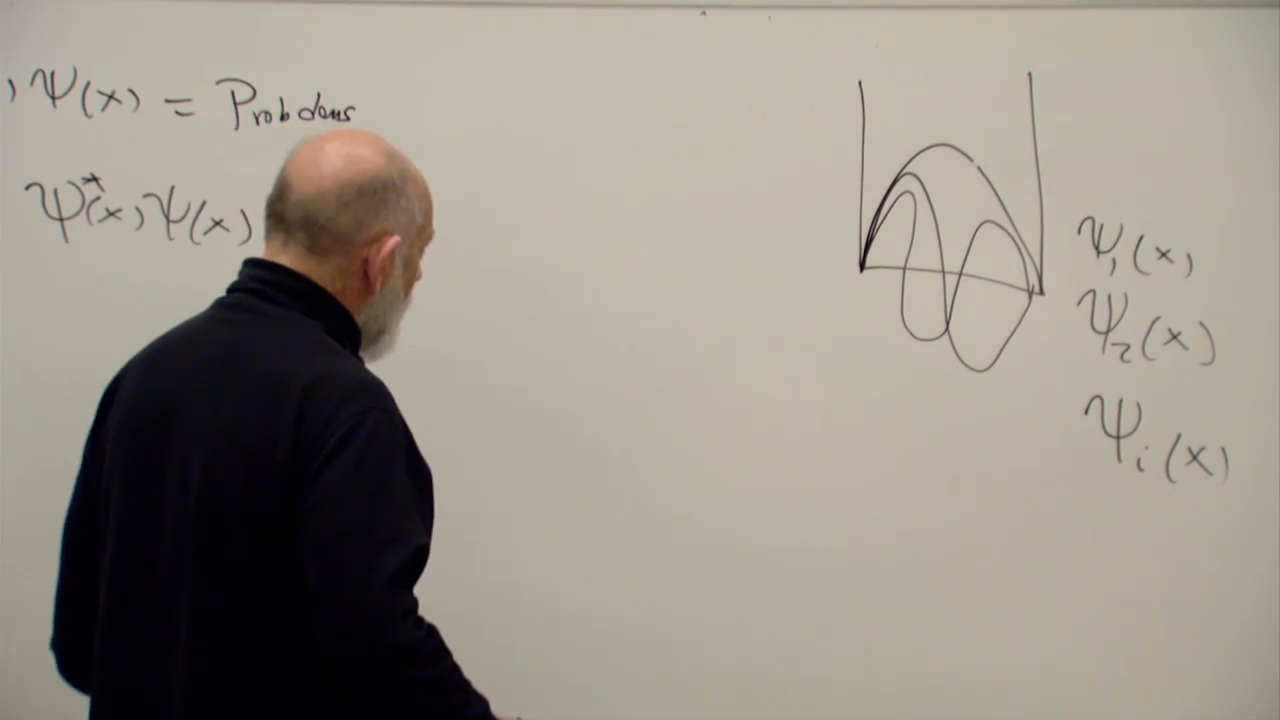
\includegraphics[width=0.94\linewidth]{lecture_07_frame_01.png}
\caption{Các mode trong hộp trên bảng giảng. Ở bên trái còn thấy mật độ Born và điều kiện chuẩn hóa của bài toán một hạt; giếng thế bên phải biểu diễn \(\psi_1(x)\), \(\psi_2(x)\) và ký hiệu tổng quát \(\psi_i(x)\).}
\lectureframe{00:08:25}
\end{figure}

Có thể tách riêng cấu trúc mode tương tự khỏi phần bị che khuất trên bảng trực tiếp:
\begin{figure}[htbp]
\centering
\begin{tikzpicture}[x=1cm,y=1cm]
  \draw[thick] (0,0) -- (0,4.0);
  \draw[thick] (7,0) -- (7,4.0);
  \draw[gray!55] (0,2.85) -- (7,2.85);
  \draw[gray!55] (0,1.35) -- (7,1.35);
  \draw[blue!75!black,thick,domain=0:7,samples=120]
    plot (\x,{2.85+0.62*sin(180*\x/7)});
  \draw[teal!70!black,thick,domain=0:7,samples=120]
    plot (\x,{1.35+0.55*sin(360*\x/7)});
  \node[right] at (7.15,3.20) {$\psi_1(x)$};
  \node[right] at (7.15,1.70) {$\psi_2(x)$};
  \node at (3.5,0.38) {$\vdots\quad\psi_i(x)$};
\end{tikzpicture}
\caption{Bản dựng lại rõ ràng của hình phác họa định tính về hộp. Các độ dời theo phương đứng chỉ nhằm tách hai hàm sóng để dễ quan sát.}
\end{figure}

Tính trực chuẩn được biểu diễn bởi
\begin{equation}
\int dx\,\psi_i^*(x)\psi_j(x)=\delta_{ij}.
\label{eq:l07-orthonormality}
\end{equation}
Nếu \(i=j\), trạng thái được chuẩn hóa và tích phân bằng một. Nếu \(i\ne j\), hai trạng thái trực giao và tích phân bằng không.

Tính đầy đủ cũng quan trọng không kém, được phát biểu như sau:
\begin{equation}
\sum_i |i\rangle\langle i|=\mathbf 1.
\label{eq:l07-resolution}
\end{equation}
Mỗi \(|i\rangle\langle i|\) chiếu lên một hướng của cơ sở; tổng trên toàn bộ cơ sở bằng toán tử đồng nhất. Khi tác dụng lên một vectơ bất kỳ, tổng này chỉ phân tích vectơ đó thành các thành phần rồi ghép lại như cũ.

Bây giờ chèn Phương trình~\eqref{eq:l07-resolution} vào giữa hai trạng thái vị trí:
\begin{align}
\langle y|x\rangle
&=\sum_i\langle y|i\rangle\langle i|x\rangle \\
&=\sum_i\psi_i(y)\psi_i^*(x) \\
&=\delta(y-x).
\label{eq:l07-position-completeness}
\end{align}
Dấu sao phải đặt trên thừa số có thứ tự bra-ket là \(\langle i|x\rangle\). Đảo thứ tự \(x\) và \(y\) sẽ cho dạng phức liên hợp nhưng tương đương. Vì vậy, mọi cơ sở trực chuẩn đầy đủ đều cung cấp một biểu diễn của hàm delta. Các hàm sin, cos, hàm sóng của dao động tử và các hàm riêng năng lượng đều đảm nhiệm cùng vai trò đó.

\begin{classroomqa}
\lecturetimestamp{00:13:43}
\audiencequestion{Trong tổng khai triển theo tính đầy đủ, hàm sóng thứ hai có cần mang dấu phức liên hợp không?}
\lecturerresponse{Có. Với thứ tự \(\langle y|i\rangle\langle i|x\rangle\), các thừa số là \(\psi_i(y)\psi_i^*(x)\). Giữ tường minh thứ tự bra-ket giúp ta không phải đoán vị trí đặt dấu sao và tránh đặt nhầm dấu.}
\end{classroomqa}

Đây là phần toán học một hạt ta cần dùng. Giờ ta chuyển sang không gian trạng thái khác.

\section{Không gian Fock: không gian trạng thái lớn hơn}

Với nhiều hạt đồng nhất, một cơ sở thuận tiện ghi lại số hạt chiếm mỗi mode một hạt:
\begin{equation}
|n_1,n_2,n_3,\ldots\rangle.
\label{eq:l07-fock-basis}
\end{equation}
Số nguyên \(n_i\) là số chiếm của mode \(i\). Ket này không phải là trạng thái một hạt được viết bằng ký hiệu cầu kỳ. Nó thuộc về một không gian Hilbert lớn hơn, chứa khu vực không hạt, mọi trạng thái một hạt, mọi trạng thái hai hạt, v.v. Không gian lớn hơn này được gọi là không gian Fock.

Để thay đổi số chiếm, với mỗi mode, ta đưa vào một toán tử tạo và một toán tử hủy,
\begin{equation}
a_i^\dagger,\qquad a_i.
\end{equation}
Toán tử thứ nhất thêm một hạt vào mode \(i\), còn toán tử thứ hai lấy đi một hạt. Ở giai đoạn này, cách nói theo dao động tử điều hòa chỉ là phương tiện ghi sổ: không nhất thiết phải có một lò xo thực sự đang dao động. Đại số dao động tử cung cấp đúng công cụ cần thiết để nâng và hạ số chiếm.

Toán tử số chiếm của mode là
\begin{equation}
\begin{aligned}
N_i&=a_i^\dagger a_i,\\
N_i|n_1,\ldots,n_i,\ldots\rangle
&=n_i|n_1,\ldots,n_i,\ldots\rangle.
\end{aligned}
\end{equation}
Chân không là
\begin{equation}
|0\rangle\equiv|0,0,0,\ldots\rangle,
\qquad
a_i|0\rangle=0
\quad\text{for every }i.
\label{eq:l07-vacuum}
\end{equation}
Vì thế, trạng thái một hạt trong mode \(i\) là
\begin{equation}
|i\rangle=a_i^\dagger|0\rangle.
\label{eq:l07-mode-created}
\end{equation}
Giờ đây, cùng ký hiệu \(|i\rangle\) có thể được hiểu là một vectơ cơ sở một hạt, hoặc là vectơ đó được nhúng vào khu vực một hạt của không gian Fock. Phép nhúng được cho bởi Phương trình~\eqref{eq:l07-mode-created}; ngữ cảnh xung quanh cho biết ta đang bàn đến không gian nào.

\section{Gộp các mode thành một trường}

Định nghĩa các trường hủy và tạo như sau:
\begin{equation}
\Psi(x)=\sum_i \psi_i(x)a_i,
\qquad
\Psi^\dagger(x)=\sum_i \psi_i^*(x)a_i^\dagger.
\label{eq:l07-field-expansion}
\end{equation}
Chữ hoa ở đây rất quan trọng. Các hàm chữ thường \(\psi_i(x)\) là những số phức; chữ hoa \(\Psi(x)\) là một toán tử trên không gian Fock. Tại mỗi điểm không gian \(x\), Phương trình~\eqref{eq:l07-field-expansion} cho một tổ hợp tuyến tính khác nhau của các toán tử mode. Đó là ý nghĩa của một hàm toán tử theo vị trí.

Với các hạt tự do, các hàm mode có thể là sóng phẳng \(e^{ikx}\). Khi đó, Phương trình~\eqref{eq:l07-field-expansion} là một khai triển Fourier, nhưng các hệ số Fourier là toán tử chứ không phải số. Thuật ngữ cũ gọi các số phức thông thường là số \(c\) và các toán tử lượng tử là số \(q\). Các hàm mode là số \(c\) và giao hoán với mọi thứ; \(a_i\) và \(a_i^\dagger\) mới mang tính chất toán tử.

Cả \(\Psi\) lẫn \(\Psi^\dagger\) đều không là toán tử Hermite. Hai toán tử là liên hợp Hermite của nhau. Hai tổ hợp
\begin{equation}
\Psi+\Psi^\dagger,
\qquad
i(\Psi^\dagger-\Psi)
\label{eq:l07-hermitian-combinations}
\end{equation}
là các toán tử Hermite và có thể biểu diễn các đại lượng quan sát được. Tuy nhiên, trước mắt, các trường hữu ích nhất với vai trò công cụ tạo, hủy và đếm hạt tại từng vị trí.

\begin{classroomqa}
\lecturetimestamp{00:21:05}
\audiencequestion{Một toán tử phụ thuộc vào \(x\) nghĩa là gì?}
\lecturerresponse{Nghĩa là mỗi giá trị của \(x\) xác định một toán tử khác nhau. Sự phụ thuộc không gian nằm trong các hàm mode thông thường, còn mỗi tổ hợp tuyến tính tạo thành tác dụng trên cùng một không gian Fock.}
\end{classroomqa}

\section{Tác dụng của trường tạo}

Một định nghĩa trở nên hữu ích khi ta hỏi nó làm gì. Bắt đầu với một trạng thái riêng vị trí trong khu vực một hạt rồi chèn phân giải đồng nhất:
\begin{align}
|x\rangle
&=\sum_i |i\rangle\langle i|x\rangle \\
&=\sum_i a_i^\dagger|0\rangle\,\psi_i^*(x) \\
&=\Psi^\dagger(x)|0\rangle.
\label{eq:l07-local-creation}
\end{align}
Vậy \(a_i^\dagger\) tạo một hạt ở mode xác định \(i\), còn \(\Psi^\dagger(x)\) tạo một hạt định xứ tại \(x\). Trong cơ sở vị trí lý tưởng hóa, sự định xứ này mang tính phân bố; một phép chuẩn bị vật lý sẽ dùng một gói sóng hẹp, nhưng ý nghĩa đại số vẫn như nhau.

\begin{classroomqa}
\lecturetimestamp{00:24:48}
\audiencequestion{\(\sum_i|i\rangle\langle i|\) có phải là một phép chiếu không?}
\lecturerresponse{Mỗi số hạng là một phép chiếu lên một trạng thái cơ sở. Tổng đầy đủ chính là toán tử đồng nhất và được gọi là phép phân giải đồng nhất. Chèn phép này không làm thay đổi trạng thái, nhưng làm lộ ra các thành phần của trạng thái trong cơ sở đã chọn.}
\end{classroomqa}

Phương trình~\eqref{eq:l07-local-creation} là cách diễn giải trực tiếp đầu tiên của trường theo hạt. Ta không chỉ gắn nhãn không gian cho một toán tử trừu tượng. Ta đã xây dựng phép toán tạo ra một hạt tại điểm không gian đó.

\begin{classroomqa}
\lecturetimestamp{00:28:20}
\audiencequestion{Trường tạo trong không gian vị trí nên mang dấu sao hay dấu dao găm?}
\lecturerresponse{Dùng dấu dao găm cho toán tử liên hợp Hermite. Dấu sao biểu thị phép liên hợp phức của các hàm sóng thông thường \(\psi_i(x)\); dấu dao găm được đặt trên \(a_i^\dagger\) và \(\Psi^\dagger(x)\).}
\end{classroomqa}

\begin{classroomqa}
\lecturetimestamp{00:28:36}
\audiencequestion{Có thể chuyển các toán tử tạo qua các hàm sóng trong khai triển theo mode không?}
\lecturerresponse{Có. Các \(\psi_i(x)\) là số \(c\) nên giao hoán với mọi toán tử. Ta chỉ cần thận trọng khi đổi thứ tự các toán tử không giao hoán, chẳng hạn \(a_i\) và \(a_j^\dagger\).}
\end{classroomqa}

\section{Từ mật độ xác suất đến mật độ hạt}

Giờ ta thử tính toán với trường. Biểu thức tự nhiên đầu tiên là
\begin{equation}
\int dx\,\Psi^\dagger(x)\Psi(x).
\end{equation}
Biểu thức này trông giống tích phân chuẩn hóa một hạt, nhưng giờ các thừa số là toán tử. Thay khai triển theo mode vào mà không đổi thứ tự các thừa số:
\begin{align}
\int dx\,\Psi^\dagger(x)\Psi(x)
&=\int dx
\left(\sum_i a_i^\dagger\psi_i^*(x)\right)\\
&\qquad\times\left(\sum_j a_j\psi_j(x)\right) \\
&=\sum_{i,j}a_i^\dagger a_j
\int dx\,\psi_i^*(x)\psi_j(x) \\
&=\sum_{i,j}a_i^\dagger a_j\,\delta_{ij} \\
&=\sum_i a_i^\dagger a_i.
\label{eq:l07-number-derivation}
\end{align}
Do đó, toán tử tổng số hạt là
\begin{equation}
N=\sum_i N_i
=\int dx\,\Psi^\dagger(x)\Psi(x).
\label{eq:l07-total-number}
\end{equation}
Với các trạng thái đang xét, những kích thích có năng lượng hữu hạn có số chiếm giảm dần về không ở các mode năng lượng đủ cao. Vì vậy, tổng này thông thường hữu hạn dù danh sách các mode khả dĩ là vô hạn.

Hàm dưới dấu tích phân là toán tử mật độ hạt cục bộ:
\begin{equation}
n(x)=\Psi^\dagger(x)\Psi(x).
\label{eq:l07-density}
\end{equation}
Nói chính xác, không thể đo mật độ tại một điểm toán học. Với một miền nhỏ \(R\), ta đo
\begin{equation}
N_R=\int_R dx\,n(x),
\label{eq:l07-regional-number}
\end{equation}
số hạt trong miền đó. Cũng như mọi đại lượng quan sát được trong cơ học lượng tử, \(N_R\) không nhất thiết có một giá trị xác định trong một trạng thái bất kỳ. Các lần chuẩn bị lặp lại có thể cho những kết quả khác nhau.

\begin{classroomqa}
\lecturetimestamp{00:36:27}
\audiencequestion{\(\Psi^\dagger(x)\Psi(x)\) có phải là mật độ xác suất nhiều hạt không?}
\lecturerresponse{Ý nghĩa trực tiếp của biểu thức này là mật độ hạt. Nói chung, biên độ xác suất nhiều hạt phụ thuộc vào tọa độ của mọi hạt. Thay vào đó, tích song tuyến tính cục bộ đếm số hạt trong một miền nhỏ khi được lấy tích phân trên miền ấy.}
\end{classroomqa}

\begin{classroomqa}
\lecturetimestamp{00:38:28}
\audiencequestion{Các toán tử \(a_i\) và \(a_i^\dagger\) chỉ tác dụng lên vectơ trạng thái, chứ không tác dụng lên các hàm sóng một hạt, đúng không?}
\lecturerresponse{Đúng. Chúng tác dụng lên các trạng thái trong không gian Fock, chẳng hạn \(|n_1,n_2,\ldots\rangle\). Các hàm mode một hạt nhân với chúng là những số thông thường, không phải đối tượng mà các toán tử nâng hạ này tác dụng lên.}
\end{classroomqa}

Các ket số chiếm tạo thành một cơ sở, chứ không phải trạng thái tổng quát nhất. Ta có thể lấy tổ hợp chồng chập của chúng, kể cả những tổ hợp trong đó cùng một tổng số hạt được phân bố khác nhau giữa các mode. Với các loại hạt trung hòa như photon, ta cũng có thể lấy chồng chập các trạng thái có tổng số hạt khác nhau. Toán tử trong Phương trình~\eqref{eq:l07-regional-number} vẫn giữ nguyên ý nghĩa thao tác trong mọi trạng thái như vậy.

\begin{classroomqa}
\lecturetimestamp{00:40:01}
\audiencequestion{Nếu chia mật độ hạt cho tổng số hạt, ta có được mật độ xác suất tìm thấy một hạt tại \(x\) không?}
\lecturerresponse{Trong một hệ có \(N\) cố định và số hạt lớn, \(N_R/N\) là tần suất tương đối và thường bám sát mật độ xác suất một hạt rất tốt. Đây không phải là một đẳng thức toán tử đồng nhất một kết quả đo với một xác suất. Số hạt đo được dao động, trong mô hình các hạt độc lập, thường ở mức cỡ \(\sqrt N\); một lần đo ngoại lệ có thể sai khác rất nhiều so với xác suất dù khả năng xảy ra lần đo ấy thấp.}
\end{classroomqa}

\begin{classroomqa}
\lecturetimestamp{00:42:25}
\audiencequestion{Điều gì xảy ra với bảo toàn điện tích khi lấy chồng chập trạng thái một electron và trạng thái không có electron?}
\lecturerresponse{Đó không phải là loại chồng chập dùng cho một khu vực cô lập có điện tích cố định. Có thể lấy chồng chập các phân bố khác nhau miễn là tổng điện tích như nhau. Photon không mang điện tích, nên các khu vực có số photon khác nhau không gây ra vấn đề như vậy. Số electron và positron cũng có thể cùng thay đổi trong khi điện tích thuần vẫn không đổi.}
\end{classroomqa}

\section{Năng lượng của các hạt độc lập}

Đại lượng quan sát được tiếp theo là năng lượng. Trước tiên, xét các hạt không tương tác với nhau. Đây thường là một phép gần đúng tốt trong hệ loãng. Về nguyên tắc, ngay cả photon cũng tương tác thông qua các quá trình bậc cao, nhưng bức xạ thông thường trong phòng thí nghiệm đủ loãng để mô tả bằng các hạt độc lập rất chính xác.

Gọi \(\omega_i\) là năng lượng của một hạt trong mode \(i\), với \(\hbar=1\). Một mode là một trạng thái một hạt. Khi đó, Hamiltonian toàn phần là
\begin{equation}
H=\sum_i\omega_i N_i
=\sum_i\omega_i a_i^\dagger a_i.
\label{eq:l07-mode-hamiltonian}
\end{equation}
Mỗi mode có hạt chiếm đóng góp năng lượng một hạt của nó một lần cho mỗi hạt.

\begin{classroomqa}
\lecturetimestamp{00:48:16}
\audiencequestion{\(\omega_i\) có phải là hàm theo vị trí không?}
\lecturerresponse{Không. Đó là trị riêng năng lượng ứng với mode \(i\). Hàm \(\psi_i(x)\) phụ thuộc vào vị trí; \(\omega_i\) phụ thuộc vào mức năng lượng được chọn.}
\end{classroomqa}

Các giá trị \(\omega_i\) được xác định từ phương trình Schrodinger độc lập thời gian của một hạt. Định nghĩa
\begin{equation}
h=-\frac{\nabla^2}{2m}+V(x).
\label{eq:l07-one-particle-h}
\end{equation}
Khi đó,
\begin{equation}
h\psi_i(x)=\omega_i\psi_i(x).
\label{eq:l07-schrodinger-eigenvalue}
\end{equation}
Trong một chiều, toán tử động lượng là \(p=-i\partial_x\), và \(p^2/(2m)\) trở thành \(-\partial_x^2/(2m)\). Trong ba chiều, ba đạo hàm bậc hai hợp lại thành \(-\nabla^2/(2m)\).

\begin{figure}[htbp]
\centering
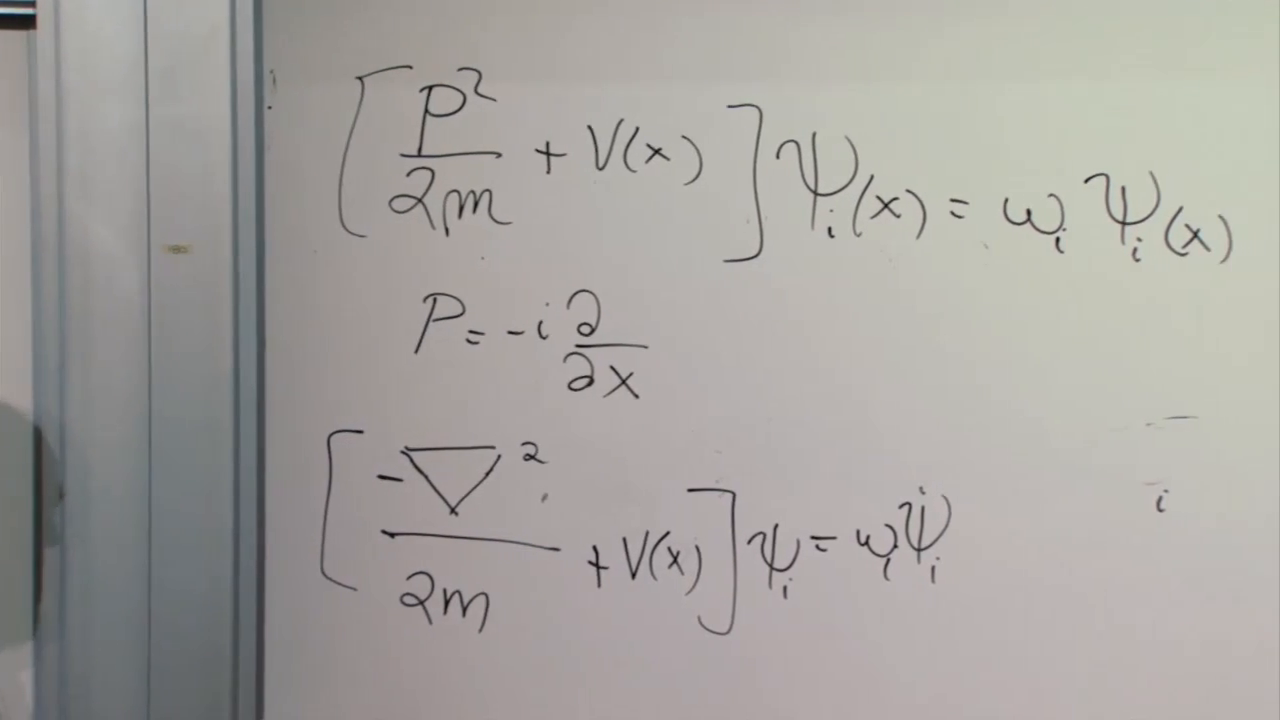
\includegraphics[width=0.94\linewidth]{lecture_07_frame_02.png}
\caption{Đoạn trên bảng chuyển từ \(p^2/(2m)+V(x)\) sang dạng vi phân của phương trình trị riêng Schrodinger một hạt. Phương trình~\eqref{eq:l07-schrodinger-eigenvalue} là bản dựng lại đã được làm rõ.}
\lectureframe{00:54:10}
\end{figure}

Với một hàm sóng một hạt chuẩn hóa bất kỳ, giá trị kỳ vọng quen thuộc là
\begin{equation}
\langle h\rangle_\psi
=\int dx\,\psi^*(x)h\psi(x).
\label{eq:l07-one-particle-energy-expectation}
\end{equation}
Công thức nhiều hạt được gợi ý bằng cách thay hàm sóng chữ thường bằng trường có giá trị toán tử. Đây chưa phải là chứng minh; đó là phỏng đoán mà giờ ta sẽ kiểm tra:
\begin{equation}
H=\int dx\,\Psi^\dagger(x)h\Psi(x).
\label{eq:l07-field-hamiltonian}
\end{equation}

\section{Viết đáp án trước, rồi chứng minh}

Thay Phương trình~\eqref{eq:l07-field-expansion} vào Hamiltonian đề xuất:
\begin{align}
\int dx\,\Psi^\dagger h\Psi
&=\int dx
\left(\sum_i a_i^\dagger\psi_i^*(x)\right)
h\left(\sum_j a_j\psi_j(x)\right) \\
&=\sum_{i,j}a_i^\dagger a_j
\int dx\,\psi_i^*(x)h\psi_j(x).
\label{eq:l07-h-expanded}
\end{align}
Toán tử vi phân \(h\) tác dụng lên hàm sóng phụ thuộc \(x\) là \(\psi_j(x)\), chứ không tác dụng lên toán tử mode \(a_j\). Theo phương trình Schrodinger,
\begin{equation}
h\psi_j(x)=\omega_j\psi_j(x).
\end{equation}
Vì thế,
\begin{align}
\int dx\,\Psi^\dagger h\Psi
&=\sum_{i,j}a_i^\dagger a_j\omega_j
\int dx\,\psi_i^*(x)\psi_j(x) \\
&=\sum_{i,j}a_i^\dagger a_j\omega_j\delta_{ij} \\
&=\sum_j\omega_j a_j^\dagger a_j.
\label{eq:l07-h-proof}
\end{align}
Đây chính là Phương trình~\eqref{eq:l07-mode-hamiltonian}. Biểu thức trường cục bộ và tổng năng lượng của mọi hạt là cùng một toán tử.

\begin{figure}[htbp]
\centering
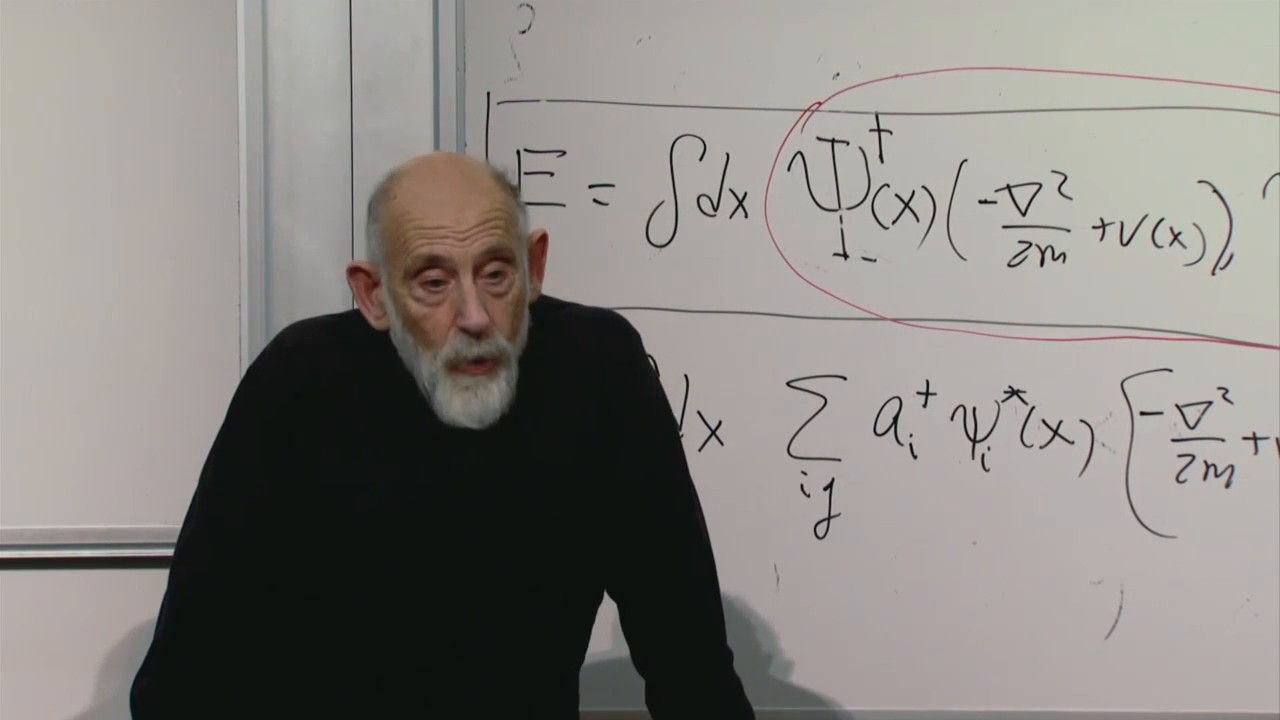
\includegraphics[width=0.94\linewidth]{lecture_07_frame_03.png}
\caption{Hamiltonian trường được nhấn mạnh trên bảng, bên dưới là phần mở đầu chứng minh bằng khai triển theo mode. Khung hình trực tiếp được giữ lại làm tư liệu; các Phương trình~\eqref{eq:l07-field-hamiltonian}--\eqref{eq:l07-h-proof} khôi phục phần biến đổi đại số đầy đủ.}
\lectureframe{01:05:34}
\end{figure}

Trong chứng minh này, không có toán tử tạo nào được đổi chỗ qua một toán tử hủy. Thứ tự \(a_i^\dagger a_j\) được giữ nguyên từ đầu đến cuối. Chỉ các hàm sóng và trị riêng là số \(c\) được tự do chuyển chỗ.

\section{Vì sao đây là một trường?}

Vì sao gọi \(\Psi(x)\) là trường? Vì đó là một đại lượng có giá trị toán tử được xác định tại mọi điểm trong không gian; các tổ hợp Hermite hoặc tích song tuyến tính xây dựng từ nó là những đại lượng quan sát được cục bộ. Mật độ \(n(x)\) và biểu thức năng lượng cục bộ bên dưới là hai ví dụ. Từ «trường» không hàm ý một tiêu chuẩn toán học bổ sung nào khác.

Trường này không phải là trường điện từ. Nó mô tả loại hạt phi tương đối tính đã cung cấp các mode một hạt và Hamiltonian \(p^2/(2m)+V\), chẳng hạn nguyên tử chuyển động chậm, neutron, proton hoặc electron. Các hạt ấy là lượng tử của trường tương ứng, theo cùng nghĩa cấu trúc như photon là lượng tử của trường điện từ.

\begin{classroomqa}
\lecturetimestamp{01:02:45}
\audiencequestion{Trong quá trình chuyển từ hệ nhiều hạt sang công thức ở trên, trường xuất hiện ở đâu?}
\lecturerresponse{Trường xuất hiện trong Phương trình~\eqref{eq:l07-field-expansion}: \(\Psi(x)\) là một toán tử tại mọi điểm trong không gian. Các phép suy ra tiếp theo cho thấy những tích cục bộ của nó đo mật độ hạt và mật độ năng lượng. Sự phụ thuộc vị trí cộng với nội dung toán tử chính là cấu trúc trường đang được xây dựng.}
\end{classroomqa}

\section{Mật độ năng lượng cục bộ}

Phương trình~\eqref{eq:l07-field-hamiltonian} viết năng lượng toàn phần thành tích phân trên không gian,
\begin{equation}
\begin{aligned}
H&=\int dx\,\mathcal H(x),\\
\mathcal H(x)
&=-\frac{1}{2m}\Psi^\dagger(x)\nabla^2\Psi(x)\\
&\quad+V(x)\Psi^\dagger(x)\Psi(x).
\end{aligned}
\label{eq:l07-hamiltonian-density}
\end{equation}
Hàm dưới dấu tích phân là một lựa chọn tự nhiên cho mật độ năng lượng cục bộ của Hamiltonian này. Dạng cục bộ không duy nhất. Chẳng hạn, tích phân từng phần biến số hạng động năng thành
\begin{equation}
\mathcal H_{\rm kin}(x)
=\frac{1}{2m}\nabla\Psi^\dagger(x)\mathbin{\cdot}\nabla\Psi(x)
\label{eq:l07-kinetic-density}
\end{equation}
ngoài một số hạng biên. Với các điều kiện biên thông thường, cả hai biểu thức đều cho cùng một Hamiltonian toàn phần. Đây là sự không đơn nhất nhỏ được nhắc đến trong bài giảng.

\begin{classroomqa}
\lecturetimestamp{01:05:57}
\audiencequestion{Có nhất thiết phải lấy tích phân mật độ năng lượng trên toàn không gian không?}
\lecturerresponse{Lấy tích phân trên toàn không gian cho năng lượng toàn phần. Lấy tích phân trên một miền nhỏ hơn cho năng lượng quy cho miền đó, tùy theo sự không đơn nhất thông thường khi chọn một mật độ cục bộ có tích phân toàn phần bằng cùng Hamiltonian.}
\end{classroomqa}

\begin{classroomqa}
\lecturetimestamp{01:06:25}
\audiencequestion{Chữ hoa \(N_i\) trong công thức năng lượng khác chữ thường \(n_i\) như thế nào?}
\lecturerresponse{\(N_i=a_i^\dagger a_i\) là một toán tử. Số nguyên \(n_i\) là một trong các trị riêng của toán tử ấy trên trạng thái số chiếm. Toán tử tác dụng lên trạng thái; trị riêng của chúng là các số thông thường.}
\end{classroomqa}

\begin{classroomqa}
\lecturetimestamp{01:06:46}
\audiencequestion{Có thể viết bản thân Hamiltonian trường dưới dạng bra hoặc ket trong ký hiệu Dirac không?}
\lecturerresponse{Không. Bra và ket biểu diễn các vectơ trạng thái và các vectơ đối ngẫu của chúng. Trường và Hamiltonian là các toán tử tác dụng lên những trạng thái đó. Giá trị kỳ vọng như \(\langle\Phi|H|\Phi\rangle\) dùng cả hai loại đối tượng và không được đồng nhất chúng với nhau.}
\end{classroomqa}

\section{Khôi phục trường hợp một hạt và tiến gần đến trường cổ điển}

Hình thức luận mở rộng bao hàm cơ học lượng tử một hạt thông thường. Hạn chế không gian Fock vào các trạng thái thỏa mãn
\begin{equation}
N|\Phi\rangle=|\Phi\rangle.
\end{equation}
Trong khu vực đó, phép xây dựng trường tái tạo mọi trạng thái một hạt và mọi dự đoán một hạt. Ta không thay thế lý thuyết cũ; ta nhúng nó vào một không gian còn mô tả được không hạt, hai hạt hoặc số hạt lớn tùy ý.

Ở phía giới hạn kia, một mode được chiếm bởi số boson rất lớn có thể ứng xử gần đúng như một sóng cổ điển. Với những trạng thái kết hợp hoặc bán cổ điển thích hợp, giá trị kỳ vọng
\begin{equation}
\Phi_{\rm cl}(x,t)=\langle\Psi(x,t)\rangle
\end{equation}
tuân theo phương trình có dạng cổ điển
\begin{equation}
i\partial_t\Phi_{\rm cl}(x,t)
=\left(-\frac{\nabla^2}{2m}+V(x)\right)\Phi_{\rm cl}(x,t)
\label{eq:l07-classical-schrodinger}
\end{equation}
đối với lý thuyết phi tương đối tính tự do. Bài giảng nêu mối liên hệ này chứ không suy ra nó. Đây là cầu nối giữa một tập hợp lượng tử và một trường sóng: số chiếm lớn làm giảm các thăng giáng tương đối, khiến những giá trị kỳ vọng thích hợp ứng xử theo cách cổ điển.

Vì vậy, hình thức luận này vừa là công cụ ghi sổ vừa mang nội dung vật lý. Nó sắp xếp mọi khu vực số hạt, đồng thời mô tả giao thoa, vướng víu và sự xuất hiện của sóng cổ điển từ các hạt lượng tử.

\begin{classroomqa}
\lecturetimestamp{01:10:43}
\audiencequestion{Vì sao có thể thao tác với các toán tử tạo và hủy trong tích phân gần như thể chúng là những số thông thường?}
\lecturerresponse{Chúng chưa bao giờ bị đổi chỗ cho nhau. Các hàm mode thông thường giao hoán với chúng, còn các đạo hàm chỉ tác dụng lên những hàm ấy. Chuyển một toán tử hủy qua một toán tử tạo sẽ đòi hỏi dùng giao hoán tử và có thể sinh thêm một số hạng; trong chứng minh này không có bước nào thực hiện phép chuyển đó.}
\end{classroomqa}

\section{Đôi lời về ký hiệu Dirac}

Một phần sự nhầm lẫn có nguồn gốc lịch sử. Hàm sóng một hạt thỏa mãn phương trình sóng và bề ngoài trông giống một trường cổ điển, nhưng đồng thời nó cũng là biên độ xác suất. Lý thuyết lượng tử thời kỳ đầu phải tách biệt hai vai trò ấy, rồi giải thích cách các trường sóng thực sự đo được, chẳng hạn trường điện từ, được cấu thành từ các lượng tử. Không gian Fock và các trường có giá trị toán tử giải quyết mâu thuẫn có vẻ tồn tại này.

Ký hiệu Dirac làm cho sự phân biệt ấy đặc biệt cô đọng. Ket thuộc về một không gian vectơ, bra thuộc về không gian đối ngẫu của nó, còn khi đặt cạnh nhau chúng tạo thành tích trong. Khi đó, phép phân giải
\begin{equation}
\sum_i|i\rangle\langle i|=\mathbf 1
\end{equation}
trở nên gần như tự giải thích. Bài giảng minh họa điều này bằng một giai thoại từ việc dạy cơ học lượng tử cho các nhà toán học: nội dung toán học vốn đã quen thuộc, nhưng ký hiệu khiến các phép biến đổi thường lệ trở nên sáng tỏ đến mức cấu trúc dường như mới mẻ. Ý ở đây không phải là một ngành thiếu khái niệm đó. Mà là ký hiệu được chọn khéo có thể khiến ta khó nhầm lẫn các phép toán hợp lệ.

Bài học ấy quan trọng ở đây. Giờ ta có một số toán tử phân biệt:
\begin{itemize}
\item \(h\) tác dụng lên các hàm sóng một hạt như một toán tử vi phân;
\item \(a_i\) và \(a_i^\dagger\) tác dụng lên các trạng thái số chiếm trong không gian Fock;
\item \(\Psi(x)\), \(\Psi^\dagger(x)\), \(N\) và \(H\) cũng tác dụng lên không gian Fock.
\end{itemize}
Khai triển trong Phương trình~\eqref{eq:l07-field-expansion} nối hai bối cảnh đầu tiên mà không nhập chúng làm một.

\begin{classroomqa}
\lecturetimestamp{01:18:16}
\audiencequestion{Các trường chỉ là hình thức luận để mô tả tập hợp các hạt thôi sao?}
\lecturerresponse{Chúng là một hình thức luận, nhưng không phải hình thức luận rỗng. Các đại lượng quan sát được cục bộ của chúng có thể đo được; các hạt là hạt lượng tử có giao thoa và vướng víu, chứ không phải những viên bi cổ điển. Các toán tử trường mã hóa chính xác những tính chất tập thể có thể đo được ấy.}
\end{classroomqa}

\section{Lưu ý về tính tương đối tính và ví dụ bên lề về điện từ}

Phép xây dựng từ đầu đến đây là phi tương đối tính. Trong vật lý tương đối tính, động lượng vẫn là một nhãn tốt cho hạt, nhưng việc định xứ vị trí hạt thật sắc nét phức tạp hơn nhiều. Vì vậy, mật độ số photon cục bộ nhìn chung không phải là một đại lượng gọn gàng như \(n(x)\) trong trường hợp phi tương đối tính. Mật độ năng lượng vẫn được xác định tốt và là đại lượng quan sát được cục bộ an toàn hơn.

Bài giảng đưa ra một phép tương tự điện từ hữu ích, được nói rõ là mang tính trực giác. Gộp điện trường và từ trường thành vectơ phức
\begin{equation}
\mathbf F=\mathbf E+i\mathbf B,
\qquad
\mathbf F^*=\mathbf E-i\mathbf B.
\label{eq:l07-riemann-silberstein}
\end{equation}
Khi đó,
\begin{equation}
\mathbf F^*\mathbin{\cdot}\mathbf F
=\mathbf E^2+\mathbf B^2,
\label{eq:l07-em-density}
\end{equation}
tỷ lệ với mật độ năng lượng điện từ theo hệ đơn vị thông thường. Đây không phải là mật độ xác suất photon theo nghĩa đen. Nên xem nó như một biến trường gọn có bình phương độ lớn đo mật độ năng lượng, hoặc nói không chính thức là mật độ photon có trọng số bằng năng lượng photon.

\begin{classroomqa}
\lecturetimestamp{01:19:10}
\audiencequestion{Có thể đồng nhất mật độ photon với cường độ điện trường không?}
\lecturerresponse{Chỉ theo nghĩa định tính và cần thận trọng. Với photon tương đối tính, số hạt cục bộ không phải là khái niệm được ưu tiên. Khẳng định vững chắc là \(E^2+B^2\) tỷ lệ với mật độ năng lượng, còn tổ hợp phức \(\mathbf E+i\mathbf B\) gộp các phương trình Maxwell thành một dạng giống phương trình Schrodinger.}
\end{classroomqa}

\begin{classroomqa}
\lecturetimestamp{01:20:09}
\audiencequestion{Vì sao hạt tương đối tính có thể có động lượng xác định nhưng vị trí lại thành vấn đề?}
\lecturerresponse{Động lượng là nhãn gọn gàng cho các biểu diễn một hạt tương đối tính, trong khi việc định xứ nghiêm ngặt xung đột với sự tạo hạt và mô tả bằng trường tương đối tính. Bài giảng này không triển khai lý thuyết đó; lưu ý này đánh dấu giới hạn của cách diễn giải mật độ phi tương đối tính đang dùng.}
\end{classroomqa}

\section{Thứ tự toán tử và hằng số năng lượng trạng thái cơ bản}

Không thể tùy tiện đổi thứ tự toán tử. Với các mode boson,
\begin{equation}
a_i a_i^\dagger=a_i^\dagger a_i+1.
\end{equation}
Vì vậy, thay thứ tự chuẩn \(\Psi^\dagger h\Psi\) bằng thứ tự đảo \((h\Psi)\Psi^\dagger\), hoặc bằng biểu thức tương ứng đã lấy tích phân một cách thích hợp, sẽ cộng thêm phần đóng góp của giao hoán tử. Trong cơ sở mode, đó là một tổng cộng thêm một lượng tử năng lượng cho mỗi mode. Đây là hằng số năng lượng trạng thái cơ bản hay năng lượng điểm không; trong giới hạn liên tục, cần có phép điều chuẩn. Bài giảng không bàn tiếp vấn đề đó ở đây, mà chỉ lưu ý rằng hai thứ tự không bằng nhau.

\begin{classroomqa}
\lecturetimestamp{01:22:04}
\audiencequestion{Khi hoán đổi \(\Psi\) và \(\Psi^\dagger\) trong Hamiltonian, điều gì xảy ra?}
\lecturerresponse{Phải tính đến giao hoán tử của chúng. Vì vậy, đảo thứ tự sẽ tạo thêm một đóng góp vào năng lượng trạng thái cơ bản, không phụ thuộc vào trạng thái, chứ không cho lại cùng một biểu thức. Hamiltonian được viết theo thứ tự chuẩn tắc, \(\Psi^\dagger h\Psi\).}
\end{classroomqa}

\section{Động lượng: phép thử cuối cùng}

Những phút cuối cùng nhắc lại phép nâng cấp ấy thêm một lần nữa. Với một hạt,
\begin{equation}
\langle p\rangle_\psi
=\int dx\,\psi^*(x)\left(-i\partial_x\right)\psi(x).
\label{eq:l07-one-particle-momentum}
\end{equation}
Thay hàm sóng bằng trường, ta thu được toán tử động lượng toàn phần
\begin{equation}
P=\int dx\,\Psi^\dagger(x)\left(-i\partial_x\right)\Psi(x),
\label{eq:l07-field-momentum}
\end{equation}
hay, trong không gian ba chiều,
\begin{equation}
\mathbf P=\int d^3x\,\Psi^\dagger(\mathbf x)
\left(-i\boldsymbol\nabla\right)\Psi(\mathbf x).
\end{equation}
Các trường mang động lượng. Một laser đủ mạnh truyền động lượng cho một bức tường và tác dụng lực lên nó; trong mô tả lượng tử, động lượng của trường là tổng động lượng của các photon.

Phương trình~\eqref{eq:l07-field-momentum} là một toán tử, không phải giá trị kỳ vọng. Khi đã cho một trạng thái trong không gian Fock \(|\Phi\rangle\), ta có thể tính
\begin{equation}
\langle P\rangle_\Phi=\langle\Phi|P|\Phi\rangle.
\end{equation}
Cần có cả toán tử lẫn trạng thái mới xác định được giá trị kỳ vọng. Nhầm lẫn giữa đại lượng quan sát được với giá trị trung bình của nó sẽ xóa nhòa chính sự phân biệt mà bài giảng đã làm sáng tỏ.

\begin{classroomqa}
\lecturetimestamp{01:26:02}
\audiencequestion{Động lượng trường được viết ở đây đã là động lượng trung bình chưa?}
\lecturerresponse{Chưa. Đây là toán tử Hermite biểu diễn đại lượng quan sát được. Hãy cho một trạng thái rồi đặt toán tử vào giữa bra và ket của trạng thái ấy để thu được giá trị kỳ vọng; kết quả đo vẫn có thể dao động quanh giá trị trung bình đó.}
\end{classroomqa}

Đây là điểm dừng tự nhiên. Bắt đầu từ các hạt, ta đã xây dựng các trường tạo và hủy cục bộ, dùng chúng để đếm hạt, rồi viết lại tổng năng lượng và động lượng của từng hạt dưới dạng các toán tử trường. Bước tiếp theo không phải là một thay đổi ký hiệu khác. Đó là dùng các toán tử trường để biểu diễn những quá trình vật lý: hạt phân rã, hạt tán xạ và các loài hạt biến đổi thành nhau.
\chapter{Pha trộn, dao động, mômen lưỡng cực điện và toán tử trường}

Ta bắt đầu hơi lệch khỏi chủ đề đã thông báo, với một câu hỏi về neutrino. Có bằng chứng cho thấy neutrino có khối lượng và các loại neutrino pha trộn với nhau. Nếu khối lượng của chúng không hoàn toàn bằng nhau, làm thế nào một loại có thể biến đổi thành loại khác mà không vi phạm định luật bảo toàn năng lượng?

Câu hỏi này gợi ra một mô hình thường gặp trong cơ học lượng tử: trạng thái dùng để chuẩn bị hoặc phát hiện một hệ không nhất thiết là trạng thái chéo hóa Hamiltonian của hệ. Trạng thái có năng lượng xác định chỉ thu nhận một pha. Còn trạng thái được chuẩn bị dưới dạng chồng chập của nhiều mức năng lượng sẽ biến đổi vì các thành phần của nó thu nhận những pha khác nhau. Sự khác biệt ấy sẽ dẫn ta từ giếng thế đôi đến dao động neutrino và sự tiến động spin. Sau một đoạn xen kẽ về mômen lưỡng cực điện của electron, ta sẽ quay lại lượng tử hóa lần hai và thấy cùng cấu trúc Fourier vị trí--động lượng ở cấp độ toán tử.

\section{Vấn đề thực sự là sự pha trộn}

Neutrino không nhất thiết đều có cùng khối lượng. Các trạng thái riêng năng lượng không pha trộn với nhau; mỗi trạng thái tiến hóa độc lập. Điều ta gọi là \emph{loại} hay hương vị của neutrino gắn với cách nó được tạo ra và được phát hiện; một trạng thái hương vị có thể là tổ hợp tuyến tính của các trạng thái riêng năng lượng-khối lượng. Có thể biểu diễn sơ đồ như sau:
\begin{equation}
|\text{type}\rangle = \sum_n c_n |E_n\rangle .
\end{equation}
Vì vậy, phát biểu đúng không phải là các trạng thái riêng năng lượng biến đổi thành nhau, mà là những trạng thái được gọi là ``neutrino electron'' hoặc ``neutrino muon'' bản thân chúng không nhất thiết là trạng thái riêng năng lượng.

\begin{classroomqa}
\lecturetimestamp{00:00:09}
\audiencequestion{Nếu neutrino có khối lượng khác nhau, chúng có thể pha trộn như thế nào trong khi năng lượng vẫn được bảo toàn?}
\lecturerresponse{Các trạng thái riêng năng lượng-khối lượng không biến đổi thành nhau. Các trạng thái hương vị electron, muon và tau là những tổ hợp tuyến tính khác nhau của các trạng thái riêng ấy. Mỗi thành phần khối lượng tiến hóa với pha riêng của nó; sự giao thoa làm thay đổi xác suất hương vị mà không vi phạm định luật bảo toàn năng lượng.}
\end{classroomqa}

Có rất nhiều ví dụ về cấu trúc này. Ví dụ dễ thấy nhất bắt đầu với một hạt trong giếng thế đôi đối xứng.

\section{Giếng thế đôi đối xứng và các trạng thái định xứ gần đúng}

Xét một hạt chuyển động trong thế năng giếng đôi đối xứng, với một hàng rào cao ngăn cách hai cực tiểu. Nếu hàng rào cao vô hạn, hai giếng trái và phải sẽ hoàn toàn tách rời. Ta có thể giải bài toán cho giếng bên trái như thể giếng bên phải không tồn tại, và tương tự cho giếng bên phải. Khi đó, các hàm sóng trạng thái cơ bản gần đúng sẽ là trạng thái định xứ bên trái \(\psi_L\) và trạng thái định xứ bên phải \(\psi_R\), cả hai có cùng năng lượng \(E\).

Trong mỗi giếng cô lập, trạng thái cơ bản có những tính chất định tính quen thuộc: trơn, không có nút và có năng lượng thấp nhất có thể khi hạt bị giam giữ. Hãy hình dung hàng rào cao ở giữa như một bức tường gạch. Coi hàng rào là vô hạn chỉ là một phép gần đúng, nhưng phép gần đúng này cho ta một cặp trạng thái định xứ hữu ích để bắt đầu.

\begin{figure}
\centering
\begin{adjustbox}{max width=\linewidth}
\begin{tikzpicture}[x=0.8cm,y=0.8cm]
\begin{scope}[shift={(-5.8,0)}]
\draw (-4,2.7) .. controls (-3.35,1.2) and (-2.55,-0.45) .. (-2.0,-0.72)
      .. controls (-1.35,-0.95) and (-0.7,0.65) .. (0,2.05)
      .. controls (0.7,0.65) and (1.35,-0.95) .. (2.0,-0.72)
      .. controls (2.55,-0.45) and (3.35,1.2) .. (4,2.7);
\draw[dashed] (-4,-0.10) -- (4,-0.10);
\node at (-3.55,-0.48) {$E$};
\draw[line width=0.9pt] (-4,-0.02) .. controls (-3.2,-0.02) and (-2.7,0.30) .. (-2.15,0.95)
      .. controls (-1.55,1.30) and (-1.15,0.35) .. (-0.55,-0.06)
      .. controls (0.15,-0.14) and (0.9,-0.15) .. (4,-0.15);
\node at (-2.15,1.35) {$\psi_L$};
\end{scope}
\begin{scope}[shift={(5.8,0)}]
\draw (-4,2.7) .. controls (-3.35,1.2) and (-2.55,-0.45) .. (-2.0,-0.72)
      .. controls (-1.35,-0.95) and (-0.7,0.65) .. (0,2.05)
      .. controls (0.7,0.65) and (1.35,-0.95) .. (2.0,-0.72)
      .. controls (2.55,-0.45) and (3.35,1.2) .. (4,2.7);
\draw[dashed] (-4,-0.10) -- (4,-0.10);
\node at (-3.55,-0.48) {$E$};
\draw[line width=0.9pt] (-4,-0.02) .. controls (-3.2,-0.01) and (-2.7,0.30) .. (-2.15,0.95)
      .. controls (-1.6,1.28) and (-1.1,0.25) .. (-0.30,-0.08)
      .. controls (0.35,-0.12) and (0.85,-0.12) .. (1.35,0.35)
      .. controls (1.9,0.88) and (2.35,1.15) .. (2.85,0.55)
      .. controls (3.2,0.05) and (3.55,-0.12) .. (4,-0.15);
\end{scope}
\end{tikzpicture}
\end{adjustbox}
\caption{Bản vẽ lại rõ nét các phác họa đầu tiên trên bảng. Hình bên trái là trạng thái thử chỉ nằm ở một phía \(\psi_L\), thu được bằng cách giả sử hàng rào hiệu dụng là vô hạn. Ở hình bên phải, cùng hàm sóng được kéo dài đối xứng qua hàng rào, minh họa sự rò qua hàng rào tuy nhỏ nhưng khác không; chính sự rò này cuối cùng tạo nên trạng thái cơ bản chẵn thực sự.}
\end{figure}

Tuy nhiên, trong cơ học lượng tử, hàng rào không thực sự vô hạn. Hàm sóng trong vùng hàng rào không chính xác bằng không; nó chỉ rất nhỏ. Sự rò rất nhỏ này chính là mấu chốt. Nó biến mô tả gần đúng trái-phải thành một bài toán pha trộn thực sự.

\section{Các trạng thái riêng parity và độ tách mức hàm mũ}

Mô tả định xứ giờ đây bị ngắt quãng bởi một định lý: nếu thế năng đối xứng, các hàm riêng năng lượng chính xác có thể được chọn sao cho chúng đối xứng hoặc phản đối xứng qua phép phản xạ.

\begin{theorem}
Nếu \(V(x)=V(-x)\) trong một chiều, thì có thể chọn các hàm riêng của Hamiltonian thỏa mãn một trong hai điều kiện
\[
\psi(x)=\psi(-x)
\qquad \text{or} \qquad
\psi(x)=-\psi(-x).
\]
\end{theorem}

Giờ là phần hiệu chỉnh. Các trạng thái một phía \(\psi_L\) và \(\psi_R\) không đối xứng cũng không phản đối xứng, nên chúng không thể là trạng thái riêng chính xác của Hamiltonian đầy đủ. Chúng chỉ là các trạng thái gần đúng tốt khi hàng rào cao. Các trạng thái riêng thực sự là những tổ hợp đối xứng và phản đối xứng,
\begin{align}
\psi_+ &= \frac{\psi_L+\psi_R}{\sqrt{2}},\\
\psi_- &= \frac{\psi_L-\psi_R}{\sqrt{2}}.
\end{align}
Dùng ký hiệu sẽ giữ nguyên trên bảng, ta ký hiệu năng lượng của chúng là
\begin{align}
H\psi_+ &= (E_1-\epsilon)\psi_+,\\
H\psi_- &= (E_1+\epsilon)\psi_-.
\end{align}
Do đó, độ tách mức tổng cộng là
\begin{equation}
\Delta E = (E_1+\epsilon)-(E_1-\epsilon)=2\epsilon .
\end{equation}

\begin{figure}[htbp]
\centering
\includegraphics[width=0.92\linewidth]{lecture_08_frame_02.png}
\caption{Hàm sóng được kéo dài đối xứng trong thế giếng đôi. Biên độ dưới hàng rào nhỏ nhưng khác không; đây là nguồn gốc của độ tách mức.}
\lectureframe{00:06:19}
\end{figure}

\begin{figure}
\centering
\begin{tikzpicture}[x=1cm,y=1cm]
\draw[->] (0,0) -- (0,3);
\node[left] at (0,2.8) {energy};
\draw (-0.35,1.60) -- (0.35,1.60);
\node[left] at (-0.45,1.60) {$\psi_L,\psi_R$};
\node at (1.7,1.60) {$\Longrightarrow$};
\draw (3.0,1.32) -- (3.75,1.32);
\draw (3.0,1.88) -- (3.75,1.88);
\draw[dashed] (2.8,1.60) -- (3.95,1.60);
\node[right] at (3.9,1.32) {$\psi_+,\ E_1-\epsilon$};
\node[right] at (3.9,1.88) {$\psi_-,\ E_1+\epsilon$};
\node[below] at (3.37,1.60) {$E_1$};
\end{tikzpicture}
\caption{Lập luận trên bảng về độ tách mức do xuyên hầm. Các trạng thái trái và phải gần đúng gần suy biến, nhưng các trạng thái riêng chẵn và lẻ chính xác bị tách nhau một lượng nhỏ \(2\epsilon\).}
\end{figure}

Thứ tự các mức thể hiện điểm cốt yếu về mặt vật lý. Trạng thái đối xứng có năng lượng thấp hơn một chút vì nó trơn hơn trong vùng hàng rào; cho phép hàm sóng rò qua và tiếp tục đối xứng làm giảm năng lượng một lượng rất nhỏ. Trạng thái phản đối xứng có năng lượng cao hơn một chút vì trạng thái kích thích thứ nhất trong một chiều có một nút, và trong bài toán đối xứng này nút nằm ở trung điểm. Độ cong tăng thêm làm tăng động năng.

Hiệu ứng này rất nhỏ, nhỏ theo hàm mũ của chiều rộng và chiều cao hàng rào. Ở đây ta không cần công thức WKB tường minh; điều quan trọng là độ tách mức có thật nhưng rất nhỏ. Cũng cần nhớ rằng dấu tổng thể của hàm sóng không mang thông tin vật lý. Thay \(\psi_-\) bằng \(-\psi_-\) không làm thay đổi trạng thái.

\section{Sự tiến hóa theo thời gian và dao động trái-phải}

Giờ hãy đặt câu hỏi về động lực học: điều gì xảy ra nếu ta đặt một hạt vào giếng bên trái? Đây là bước quyết định, vì dao động là biểu hiện phụ thuộc thời gian của chính hiện tượng pha trộn ấy.

Các hệ thức ngược là
\begin{align}
\psi_L &= \frac{\psi_+ + \psi_-}{\sqrt{2}},\\
\psi_R &= \frac{\psi_+ - \psi_-}{\sqrt{2}}.
\end{align}
Vậy trạng thái ban đầu định xứ bên trái là
\begin{equation}
\psi(0)=\psi_L=\frac{\psi_+ + \psi_-}{\sqrt{2}}.
\end{equation}
Đây không phải trạng thái riêng năng lượng, nên nó phải tiến hóa một cách không tầm thường.

Ta dùng quy ước Schr\"odinger chuẩn \(e^{-iEt}\). Một pha chung không gây ra hiệu ứng quan sát được; chỉ có pha tương đối giữa hai thành phần năng lượng mới có thể chuyển xác suất từ giếng này sang giếng kia.

Theo quy ước đó,
\begin{equation}
\psi(t)=\frac{1}{\sqrt{2}}\left(e^{-i(E_1-\epsilon)t}\psi_+ + e^{-i(E_1+\epsilon)t}\psi_-\right).
\end{equation}
Đây là phiên bản đã chỉnh lý của công thức trên bảng. Bây giờ ta đặt pha chung ra ngoài:
\begin{equation}
\psi(t)=\frac{e^{-iE_1 t}}{\sqrt{2}}\left(e^{i\epsilon t}\psi_+ + e^{-i\epsilon t}\psi_-\right).
\end{equation}
Một pha giờ quay theo một chiều quanh đường tròn đơn vị, pha kia quay theo chiều ngược lại. Trạng thái chỉ thay đổi vì hai pha này lệch nhịp với nhau.

Để thấy rõ dao động trái-phải, thay các định nghĩa của \(\psi_\pm\) vào biểu thức:
\begin{align}
\psi(t)
&= \frac{e^{-iE_1 t}}{2}
\left[e^{i\epsilon t}(\psi_L+\psi_R)+e^{-i\epsilon t}(\psi_L-\psi_R)\right] \\
&= \frac{e^{-iE_1 t}}{2}
\left[(e^{i\epsilon t}+e^{-i\epsilon t})\psi_L+(e^{i\epsilon t}-e^{-i\epsilon t})\psi_R\right] \\
&= e^{-iE_1 t}\left[\psi_L\cos(\epsilon t)+i\,\psi_R\sin(\epsilon t)\right].
\end{align}
Đây là phần suy diễn có lời giải then chốt của chương. Trong phép gần đúng hai trạng thái, với \(\psi_L\) và \(\psi_R\) trực chuẩn, xác suất là
\begin{equation}
P_L(t)=\cos^2(\epsilon t),
\qquad
P_R(t)=\sin^2(\epsilon t).
\end{equation}
Vì vậy, hệ dao động. Ở những thời điểm trung gian, trạng thái thực sự là một chồng chập; chẳng hạn, khi \(\epsilon t=\pi/4\), xác suất ở hai phía bằng nhau. Các pha tiến hóa liên tục, và trạng thái định xứ cũng thay đổi liên tục theo chúng.

Phần suy diễn trên bảng xác định thời điểm đầu tiên mà dấu tương đối đổi chiều. Ta tìm thời điểm sao cho
\begin{equation}
e^{-i\epsilon t}=-\,e^{i\epsilon t},
\end{equation}
đây là mốc dễ thấy trên bảng. Nhân hai vế ta được
\begin{equation}
e^{2i\epsilon t}=-1.
\end{equation}
Ở lần đầu tiên điều này xảy ra,
\begin{equation}
2\epsilon t=\pi,
\qquad\text{so}\qquad
t_{L\to R}=\frac{\pi}{2\epsilon}.
\end{equation}

\begin{figure}[htbp]
\centering
\includegraphics[width=0.94\linewidth]{lecture_08_frame_05.png}
\caption{Tính toán pha tương đối trên bảng. Hai thành phần năng lượng trở nên ngược pha khi \(e^{2i\epsilon t}=-1\), cho thời gian chuyển trạng thái lần đầu \(2\epsilon t=\pi\). Phần suy diễn được trình bày bằng chữ dùng nhất quán quy ước pha Schr\"odinger.}
\lectureframe{00:17:52}
\end{figure}
Tại thời điểm đó,
\begin{equation}
\psi(t_{L\to R}) \propto \frac{\psi_+-\psi_-}{\sqrt{2}}=\psi_R.
\end{equation}
Pha tổng thể không quan trọng. Điều cốt yếu là hạt ban đầu được đặt ở bên trái đã tiến hóa thành trạng thái định xứ bên phải. Sau một khoảng thời gian bằng như vậy nữa, nó lại dao động trở về. Pha trộn và dao động luôn đi cùng nhau.

Phương trình rất rõ ràng: \(\epsilon\) nhỏ thì dao động chậm và thời gian chuyển trạng thái dài. Không trạng thái định xứ nào có năng lượng xác định, nhưng hai thành phần năng lượng chính xác vẫn bảo toàn năng lượng và tiến hóa đúng như dự kiến.

\section{Các phép tương tự với neutrino, amoniac và spin}

Giếng đôi cung cấp cho ta khuôn mẫu để hiểu câu hỏi ban đầu về neutrino. Neutrino được tạo ra cùng với một electron được gọi là neutrino electron; neutrino được tạo ra cùng với một muon được gọi là neutrino muon. Các nhãn hương vị này mô tả các kênh tạo ra và phát hiện neutrino. Một cơ sở khác gồm các trạng thái có khối lượng xác định, và do đó có năng lượng hạt tự do xác định khi động lượng cố định.

Trong mô hình minh họa đơn giản nhất gồm hai trạng thái pha trộn cực đại,
\begin{equation}
|\nu_e\rangle \sim \frac{|m_1\rangle+|m_2\rangle}{\sqrt{2}},
\qquad
|\nu_\mu\rangle \sim \frac{|m_1\rangle-|m_2\rangle}{\sqrt{2}},
\end{equation}
trong đó các trạng thái riêng khối lượng đóng vai trò của \(\psi_+\) và \(\psi_-\), còn các trạng thái hương vị đóng vai trò của \(\psi_L\) và \(\psi_R\). Sự pha trộn neutrino thực tế dùng một ma trận pha trộn không tầm thường thay cho các hệ số bằng nhau này, nhưng cơ chế đã thể hiện rõ ở đây.

Neutrino electron được tạo ra trong một quá trình có electron tham gia, cũng như một hạt có thể được đặt vào giếng bên trái. Trong một quãng đường ngắn, hai thành phần khối lượng của nó tích lũy các pha gần như bằng nhau, nên khi tương tác, nó vẫn được nhận diện là có hương vị electron. Sau khi truyền đi một quãng đường dài, các pha của chúng tách biệt. Khi đó, tương tác dòng tích điện về sau có thể tạo ra muon thay vì electron: trạng thái đã có thêm thành phần hương vị muon. Lặp lại thí nghiệm ở các khoảng cách hoặc năng lượng khác nhau sẽ cho thấy dao động.

Điều này không mâu thuẫn với định luật bảo toàn năng lượng. Các trạng thái riêng năng lượng-khối lượng làm đúng như những gì được kỳ vọng ở trạng thái riêng. Chính chồng chập hương vị mới tiến hóa. Trong giới hạn tương đối tính, pha tương đối quan sát được phụ thuộc vào hiệu bình phương khối lượng, có dạng sơ đồ như sau
\begin{equation}
\Delta\phi_{ij}\simeq \frac{\Delta m_{ij}^{,2}L}{2E}.
\end{equation}
Do đó, dao động cho thấy không phải mọi khối lượng neutrino đều giống hệt nhau; ít nhất hai trạng thái riêng khối lượng có khối lượng khác nhau.

\begin{classroomqa}
\lecturetimestamp{00:24:06}
\audiencequestion{Điều gì quyết định độ tách nhỏ \(\epsilon\) trong ví dụ giếng đôi?}
\lecturerresponse{Độ tách này phụ thuộc vào khối lượng hạt, cũng như chiều cao và chiều rộng của hàng rào. Xuyên hầm phụ thuộc theo hàm mũ vào những đặc điểm ấy, nên chỉ cần thay đổi hàng rào vừa phải cũng có thể làm thay đổi lớn theo tỷ lệ của \(\epsilon\).}
\end{classroomqa}

\begin{classroomqa}
\lecturetimestamp{00:24:26}
\audiencequestion{Hiện tượng dao động này đã thực sự được quan sát chưa?}
\lecturerresponse{Có. Độ tách mức do xuyên hầm được quan sát trong các hệ lượng tử thông thường, còn dao động hương vị được quan sát ở neutrino. Cơ chế vi mô khác nhau, nhưng cả hai đều thể hiện cùng kiểu tiến hóa pha của hệ hai trạng thái.}
\end{classroomqa}

\begin{classroomqa}
\lecturetimestamp{00:24:34}
\audiencequestion{Dao động neutrino liên hệ thế nào với khối lượng neutrino?}
\lecturerresponse{Các trạng thái riêng truyền đi có khối lượng khác nhau nên tích lũy các pha khác nhau. Sự giao thoa giữa chúng làm thay đổi thành phần hương vị. Trong mô tả tương đối tính thực tế, hiệu bình phương khối lượng mới chi phối dao động, chứ không phải khối lượng của một hạt biến thiên theo thời gian theo nghĩa đen.}
\end{classroomqa}

\begin{classroomqa}
\lecturetimestamp{00:25:02}
\audiencequestion{Khối lượng neutrino chỉ là lý thuyết đang chiếm ưu thế, hay là sự thật thực nghiệm?}
\lecturerresponse{Dao động là sự thật thực nghiệm và đòi hỏi các hiệu khối lượng khác không. Thang khối lượng tuyệt đối là một đại lượng riêng biệt và khó đo hơn, nhưng bức tranh tối giản trong đó mọi neutrino đều không có khối lượng đã bị thực nghiệm bác bỏ.}
\end{classroomqa}

\subsection{Sự nghịch đảo của amoniac: một hàng rào theo nghĩa đen}

Phân tử amoniac, \(\mathrm{NH}_3\), có dạng chóp tam giác: ba nguyên tử hydro nằm trên một mặt phẳng, còn nitơ ở một phía của mặt phẳng đó. Có một cấu hình tương đương trong đó nitơ ở phía bên kia. Hai cấu hình định xứ này không phải các trạng thái dừng chính xác. Nitơ có thể xuyên hầm qua mặt phẳng hydro, tạo ra các trạng thái riêng năng lượng đối xứng và phản đối xứng, cùng độ tách mức nghịch đảo nhỏ. Đây là nguồn gốc vật lý của chính toán học ấy trong maser amoniac.

\begin{classroomqa}
\lecturetimestamp{00:25:11}
\audiencequestion{Trong amoniac, hàng rào có phải là cấu hình trong đó nitơ đi qua mặt phẳng hydro không?}
\lecturerresponse{Đúng. Năng lượng phân tử đạt cực tiểu ở mỗi cấu hình dạng chóp, còn cấu hình phẳng có năng lượng cao hơn. Xuyên hầm qua cấu hình đó ghép nối hai phía.}
\end{classroomqa}

\begin{classroomqa}
\lecturetimestamp{00:27:10}
\audiencequestion{Hàng rào vật lý tương ứng giữa neutrino electron và neutrino muon là gì?}
\lecturerresponse{Không có hàng rào không gian theo nghĩa đen. Phép tương tự ở đây là về mặt đại số: một tương tác ngoài đường chéo trong Hamiltonian neutrino làm pha trộn cơ sở hương vị. Trong amoniac, tương tác đó bắt nguồn từ xuyên hầm; với neutrino, nó là một phần của cấu trúc khối lượng và pha trộn.}
\end{classroomqa}

\subsection{Sự tiến động spin: pha trộn không cần xuyên hầm}

Ta đã gặp cùng một cấu trúc đại số ở spin. Xét hai trạng thái \(|\uparrow_z\rangle\) và \(|\downarrow_z\rangle\). Khi không có từ trường, chúng suy biến. Bây giờ bật từ trường theo hướng \(x\). Các trạng thái riêng năng lượng không còn là các trạng thái riêng \(z\), mà là các trạng thái phân cực theo \(x\). Dùng tạm các tên trái--phải trên bảng,
\begin{align}
|L_x\rangle &= \frac{|\uparrow_z\rangle+|\downarrow_z\rangle}{\sqrt{2}},\\
|R_x\rangle &= \frac{|\uparrow_z\rangle-|\downarrow_z\rangle}{\sqrt{2}}.
\end{align}
Đây là các trạng thái tương tự trực tiếp với \(\psi_+\) và \(\psi_-\). Mômen từ song song và đối song song với từ trường có năng lượng hơi khác nhau. Nếu các năng lượng ấy là \(E\mp\epsilon\), thì spin ban đầu hướng lên tiến hóa như sau
\begin{equation}
|\uparrow_z,t\rangle
= e^{-iEt}\left[\cos(\epsilon t)\,|\uparrow_z\rangle
+ i\sin(\epsilon t)\,|\downarrow_z\rangle\right].
\end{equation}
Đây là cùng công thức như với giếng đôi, chỉ khác là giờ đây sự tiến hóa liên tục là sự tiến động spin quanh trục \(x\). Bắt đầu từ \(+z\), spin đi qua các hướng ngang, đạt \(-z\) sau nửa chu kỳ tiến động, rồi trở lại sau nửa chu kỳ nữa. Phép đo \(S_z\) vẫn chỉ cho kết quả lên hoặc xuống; trạng thái spin biến thiên liên tục quyết định xác suất thu được mỗi kết quả. Cơ chế này không cần xuyên hầm. Điều kiện duy nhất là Hamiltonian phải chéo trong một cơ sở khác với cơ sở dùng để chuẩn bị trạng thái.

\begin{classroomqa}
\lecturetimestamp{00:32:25}
\audiencequestion{Trong bức tranh này, neutrino tau ra sao?}
\lecturerresponse{Nó cũng pha trộn. Bài toán thực có ba trạng thái hương vị và ba trạng thái khối lượng, nên một ma trận pha trộn ba nhân ba thay cho phép quay hai trạng thái. Nguyên lý giao thoa pha vẫn không đổi.}
\end{classroomqa}

\begin{classroomqa}
\lecturetimestamp{00:32:57}
\audiencequestion{Ngay sau khi áp dụng từ trường ngang, spin vẫn hướng lên chứ, và nó có thể hướng về phía chúng ta hoặc ra xa chúng ta không?}
\lecturerresponse{Trong khoảng thời gian rất ngắn, gần như chắc chắn spin vẫn hướng lên, với xác suất hướng xuống nhỏ. Trạng thái tiến động liên tục quanh trục từ trường và đi qua các hướng ngang \(\pm y\), đồng thời vẫn vuông góc với từ trường hướng theo \(x\) nếu ban đầu nó vuông góc với từ trường. Phép đo theo bất kỳ trục tùy chọn nào vẫn cho một trong các trị riêng rời rạc của trục đó.}
\end{classroomqa}

\begin{classroomqa}
\lecturetimestamp{00:34:30}
\audiencequestion{Có phải ta chọn từ trường yếu để spin không bao giờ hướng dọc theo từ trường không?}
\lecturerresponse{Không. Hình học của chuyển động là hệ quả của sự tiến động quanh trục từ trường, chứ không phải do từ trường yếu. Từ trường yếu chỉ làm độ tách năng lượng và tần số tiến động nhỏ đi, khiến dao động chậm, tương tự ví dụ neutrino.}
\end{classroomqa}

Độ mạnh pha trộn neutrino và khối lượng nhỏ của neutrino là những tham số mà Mô hình Chuẩn tối giản theo cách xây dựng ban đầu không giải thích được nguồn gốc sâu xa. Vì thế, khối lượng neutrino cho thấy vật lý vượt ra ngoài mô hình tối giản ấy, dù thang đo quan sát được rất nhỏ và có thể phản ánh vật lý ở một thang năng lượng rất xa.

\begin{classroomqa}
\lecturetimestamp{00:36:27}
\audiencequestion{Có phải nhờ hiện tượng dao động mà ta biết neutrino có khối lượng không?}
\lecturerresponse{Đây là bằng chứng trực tiếp có tính quyết định cho thấy các thành phần truyền đi có khối lượng khác nhau. Nếu mọi thành phần liên quan đều chính xác không có khối lượng và suy biến, chúng sẽ không tích lũy pha tương đối phụ thuộc khối lượng, và sẽ không có kiểu dao động hương vị trong chân không này.}
\end{classroomqa}

\begin{classroomqa}
\lecturetimestamp{00:37:57}
\audiencequestion{Sau nửa chu kỳ, neutrino có nên biểu hiện một nửa như hương vị electron và một nửa như hương vị muon không?}
\lecturerresponse{Trong mô hình lý tưởng đối xứng hai trạng thái, xác suất bằng nhau xuất hiện tại một phần tư chu kỳ xác suất đầy đủ, còn sự chuyển đổi hoàn toàn xảy ra tại cực đại đầu tiên. Dao động ba hương vị thực có các góc pha trộn không bằng nhau, nhiều tần số, các ràng buộc spin-độ xoắn và hiệu ứng vật chất, nên sự chuyển đổi đối xứng hoàn toàn không phải là trường hợp tổng quát.}
\end{classroomqa}

\begin{classroomqa}
\lecturetimestamp{00:38:36}
\audiencequestion{Nếu các thành phần khối lượng khác nhau, vận tốc của neutrino Mặt Trời có nhất thiết phải thay đổi để bảo toàn động lượng không?}
\lecturerresponse{Trạng thái hương vị là chồng chập kết hợp của các thành phần có khối lượng cố định; khối lượng của nó không phải một đại lượng cổ điển dao động theo thời gian. Trong mô tả thường dùng với động lượng bằng nhau, các thành phần có năng lượng và vận tốc nhóm hơi khác nhau; còn trong mô tả năng lượng bằng nhau, chúng có động lượng hơi khác nhau. Nếu được xử lý nhất quán, cả hai quy ước đều cho cùng pha dao động quan sát được.}
\end{classroomqa}

Sự tiến hóa pha này đã giải quyết sự thiếu hụt neutrino Mặt Trời từng được phát hiện trước đây. Các máy dò đời đầu chủ yếu nhạy với neutrino electron, nên neutrino rời Mặt Trời dưới dạng hương vị electron có thể đến nơi một phần mang hương vị muon hoặc tau và không được ghi nhận qua kênh đó. Tính toán chi tiết về Mặt Trời bao gồm sự pha trộn ba hương vị và hiệu ứng vật chất, nhưng bài học khái niệm đã có trong giếng đôi: việc chuẩn bị và sự truyền đi sử dụng các cơ sở khác nhau.

\section{Đoạn xen kẽ: mômen lưỡng cực điện, tính đối xứng và khẳng định ``“Hình cầu electron”''}

Vì ta đang bàn về hiện tượng học hạt, hãy tạm rời toán học hình thức. Một bài viết đại chúng mô tả giới hạn mới về mômen lưỡng cực điện của electron bằng cách nói rằng electron đã được chứng minh là hình cầu. Khẩu hiệu ấy nhập nhằng ba câu hỏi khác nhau: mômen lưỡng cực điện đo đại lượng gì, tính đối xứng quay có nghĩa gì đối với một trạng thái lượng tử, và thí nghiệm thực sự đã đặt ra giới hạn nào.

\subsection{Đại lượng nào đã được đo?}

Đại lượng được đo, hay đúng hơn là được đặt giới hạn, là mômen lưỡng cực điện của electron. Với các điện tích tách rời \(\pm q\), mômen lưỡng cực là
\begin{equation}
\mathbf d = q\,\boldsymbol{\ell},
\end{equation}
trong đó \(\boldsymbol{\ell}\) là vectơ phân cách. Mômen lưỡng cực khác không có nghĩa là phân bố điện tích bị lệch so với một tâm nào đó.

Tuy nhiên, với electron, câu hỏi thích hợp không chỉ là điện tích có lệch tâm theo một hướng tùy ý nào đó hay không. Electron có spin, do đó có một trục. Nó cũng có mômen từ. Câu hỏi có ý nghĩa vật lý là liệu có tương quan giữa độ lệch của điện tích và trục ấy hay không:
\begin{equation}
\mathbf d_e \parallel \boldsymbol{\mu}_e
\qquad \text{or equivalently} \qquad
\mathbf d_e \parallel \mathbf S .
\end{equation}
Đó chính là điều được gọi là mômen lưỡng cực điện của electron. Về mặt khái niệm, ta xét xem đặt một electron phân cực spin trong điện trường có làm tách hai định hướng spin hay không:
\begin{equation}
H_{\mathrm{EDM}}=-\mathbf d_e\cdot \mathbf E,
\qquad
\mathbf d_e=d_e\frac{\mathbf S}{|\mathbf S|}.
\end{equation}
Thí nghiệm thực tế trên bàn thí nghiệm tinh vi hơn nhiều so với hình dung một electron trần nằm giữa hai bản tụ điện, nhưng đây là ý tưởng về tính đối xứng và độ dịch chuyển năng lượng mà thí nghiệm khai thác.

\subsection{Vì sao không có mômen lưỡng cực điện không đồng nghĩa với hình cầu}

Điều chỉnh đầu tiên rất cơ bản. Một vật có thể không có mômen lưỡng cực mà vẫn không có dạng cầu. Một ellipsoid có tâm trùng với tâm điện tích có lượng điện tích ở mỗi phía bằng nhau nên không có lưỡng cực, nhưng vẫn có thể có mômen tứ cực. Một phân bố phức tạp hơn nữa có thể không có mômen lưỡng cực cũng không có mômen tứ cực, nhưng vẫn có mômen đa cực bậc cao hơn. Đo một hệ số đa cực không thể xác định toàn bộ hình dạng.

Trong cơ học lượng tử, từ ``hình dạng'' trở nên tinh tế hơn. Hãy hình dung một phân tử giống quả tạ gồm hai nguyên tử, với độ dài liên kết gần như cố định. Bỏ qua dao động xuyên tâm và chỉ xét chuyển động quay. Các trạng thái quay được xác định bởi mômen động lượng. Nếu phân tử là boson, trạng thái quay thấp nhất có \(J=0\). Vì mômen động lượng sinh ra phép quay,
\begin{equation}
\begin{gathered}
J=0 \quad\Longrightarrow\\
\text{rotationally invariant ground state.}
\end{gathered}
\end{equation}
trạng thái lượng tử bất biến qua phép quay, dù mọi hình dung theo một định hướng xác định đều trông như quả tạ. Có thể mô tả trạng thái này là chồng chập kết hợp của mọi định hướng. Gọi trạng thái là ``hình cầu'' hữu ích đối với một số phép đo nhưng có thể gây hiểu lầm đối với những phép đo khác.

Hãy chụp nhanh một ảnh. Chụp nhanh ở đây là phép đo định hướng; phép đo định hướng đủ chính xác đưa hệ vào trạng thái định xứ theo góc. Trạng thái như vậy không thể đồng thời có mômen động lượng xác định. Đây là dạng quay của nguyên lý bất định vị trí--động lượng: định xứ góc tất yếu làm xuất hiện độ trải của mômen động lượng, do đó kích thích chuyển động quay.

Với một vật quay cứng,
\begin{equation}
E_J=\frac{J(J+1)}{2I},
\end{equation}
như vậy năng lượng cần để phân giải cấu trúc phụ thuộc vào mômen quán tính \(I\). Một quả tạ dùng trong phòng tập có \(I\) rất lớn và các mức quay cách nhau cực kỳ sít; ánh sáng thông thường có thể dễ dàng làm nhiễu nó đủ để bộc lộ một định hướng. Các mức của phân tử cách nhau xa hơn. Các mức của hadron gọn đặc còn cách xa hơn nhiều. Nếu đầu dò không đủ năng lượng để kích thích cấu trúc quay đầu tiên có thể phân giải, các phép đo lặp lại chỉ thấy trạng thái cơ bản đã lấy trung bình theo phép quay.

Có thể hình dung meson một cách sơ lược như một hệ hai hạt gồm quark--phản quark. Các kích thích quỹ đạo đầu tiên cần năng lượng hàng trăm triệu electron vôn hoặc hơn, cao hơn rất nhiều so với năng lượng của photon quang học. Vì thế, đầu dò năng lượng thấp không thể chụp nhanh để thấy định hướng bên trong. ``Có hình cầu hay không'' một phần phụ thuộc vào trạng thái được chuẩn bị và một phần vào độ phân giải của thiết bị.

Electron làm vấn đề này rõ hơn. Đây là hạt có spin-\(\tfrac12\), chứ không phải một đại lượng vô hướng quay. Trạng thái phân cực spin mang một trục và một mômen từ. Hình dung quen thuộc về điện tích quay quanh trục ấy chỉ là một cách diễn giải gợi hình---hạt Dirac dạng điểm không thực sự là một quả cầu nhỏ đang quay---nhưng cách hình dung này nhắc đúng rằng mômen từ đổi chiều khi spin đổi chiều. Câu hỏi về mômen lưỡng cực điện là liệu độ lệch của điện tích có tương quan với chính trục ấy hay không. Kết quả bằng không không biến electron thành một quả cầu cổ điển.

\begin{classroomqa}
\lecturetimestamp{00:57:30}
\audiencequestion{Nếu một phần điện tích của electron bị dịch chuyển, điều đó có vi phạm tính lượng tử hóa điện tích không?}
\lecturerresponse{Không. Tính lượng tử hóa điện tích ấn định tổng điện tích. Mômen lưỡng cực liên quan đến mômen không gian bậc nhất của phân bố điện tích đó, hoặc tương đương là một tương tác được phép giữa hạt điểm với điện trường; nó không đòi hỏi tổng điện tích phải thay đổi một lượng phân số.}
\end{classroomqa}

\begin{classroomqa}
\lecturetimestamp{00:58:00}
\audiencequestion{Mômen lưỡng cực điện có bị lý thuyết trường lượng tử cấm không?}
\lecturerresponse{Bản thân lý thuyết trường lượng tử không cấm chúng. Chúng bị cấm khi một số đối xứng rời rạc nhất định là chính xác. Khi các đối xứng ấy bị vi phạm, toán tử mômen lưỡng cực điện được phép xuất hiện, dù hệ số của nó có thể cực kỳ nhỏ.}
\end{classroomqa}

\subsection{Tính chẵn lẻ và phép đảo ngược thời gian}

Nội dung thực sự của phần thảo luận về mômen lưỡng cực điện là tính đối xứng. Dưới phép biến đổi chẵn lẻ, mômen lưỡng cực điện biến đổi như một vectơ cực thông thường, còn mômen từ biến đổi như một vectơ trục:
\begin{align}
P:\qquad &\mathbf d_e \to -\mathbf d_e,
&\boldsymbol{\mu}_e \to \boldsymbol{\mu}_e .
\end{align}
Dưới phép đảo ngược thời gian, dòng điện tuần hoàn xác định mômen từ đổi chiều, còn độ lệch tĩnh của điện tích thì không:
\begin{align}
T:\qquad &\mathbf d_e \to \mathbf d_e,
&\boldsymbol{\mu}_e \to -\boldsymbol{\mu}_e .
\end{align}
Vì vậy, một mômen lưỡng cực điện khác không, song song với trục spin của electron, bị cấm nếu đối xứng chẵn lẻ là chính xác, và cũng bị cấm nếu đối xứng đảo ngược thời gian là chính xác:
\begin{equation}
(P\ \text{exact}) \Rightarrow \mathbf d_e=0,
\qquad
(T\ \text{exact}) \Rightarrow \mathbf d_e=0.
\end{equation}

Cần nói rõ hình học ở đây. Mômen từ được tạo ra bởi dòng điện chạy thành vòng. Phép phản xạ gương đảo chiều các vectơ cực thông thường, nhưng giữ nguyên vectơ trục vuông góc với vòng dây đó. Độ dời điện tích dọc theo trục thì đổi chiều. Vì vậy, electron có \(\mathbf d_e\) song song với \(\boldsymbol\mu_e\) sẽ bị phản xạ thành electron có cùng chiều mômen từ nhưng quan hệ giữa mômen điện và mômen từ thì ngược lại. Nếu đối xứng chẵn lẻ là chính xác và chỉ có một loại electron, thì hai mô tả này phải biểu diễn cùng một hạt; chỉ \(d_e=0\) là phù hợp.

Phép đảo ngược thời gian dẫn đến cùng kết luận theo một cách khác. Chiếu cuộn phim ngược chiều thời gian làm dòng điện đổi chiều, do đó \(\boldsymbol\mu_e\) cũng đổi chiều, nhưng không làm độ dời điện tích tĩnh chuyển động. Một trạng thái có hai mômen song song biến thành trạng thái có hai mômen ngược chiều. Đối xứng đảo ngược thời gian chính xác cũng sẽ đòi hỏi \(d_e=0\).

\begin{figure}[htbp]\centering
\begin{tikzpicture}[>=Stealth,scale=0.95]
  \node[font=\bfseries] at (1.0,2.25) {original};
  \draw[->,very thick,blue!70!black] (0.65,0) -- (0.65,1.65);
  \draw[->,very thick,red!75!black] (1.35,0) -- (1.35,1.65);
  \node[blue!70!black,below] at (0.65,0) {$\boldsymbol\mu$};
  \node[red!75!black,below] at (1.35,0) {$\mathbf d$};

  \node[font=\bfseries] at (4.5,2.25) {parity};
  \draw[->,very thick,blue!70!black] (4.15,0) -- (4.15,1.65);
  \draw[->,very thick,red!75!black] (4.85,1.65) -- (4.85,0);
  \node[blue!70!black,below] at (4.15,0) {$\boldsymbol\mu$};
  \node[red!75!black,below] at (4.85,0) {$-\mathbf d$};

  \node[font=\bfseries] at (8.0,2.25) {time reversal};
  \draw[->,very thick,blue!70!black] (7.65,1.65) -- (7.65,0);
  \draw[->,very thick,red!75!black] (8.35,0) -- (8.35,1.65);
  \node[blue!70!black,below] at (7.65,0) {$-\boldsymbol\mu$};
  \node[red!75!black,below] at (8.35,0) {$\mathbf d$};
\end{tikzpicture}\caption{Phép kiểm tra đối xứng được dựng lại từ lập luận trên bảng. Phép biến đổi chẵn lẻ đảo chiều mômen lưỡng cực điện nhưng không đảo chiều mômen từ dạng vectơ trục; phép đảo ngược thời gian đảo chiều mômen từ nhưng không đảo chiều độ dời điện tích tĩnh. Nếu một trong hai đối xứng là chính xác, mômen lưỡng cực điện vĩnh cửu song song với spin sẽ bị cấm.}\end{figure}

\begin{figure}[htbp]\centering
\includegraphics[width=0.94\linewidth]{lecture_08_frame_06.png}\caption{Các hình phác họa trục từ và độ dời điện tích đặt cạnh nhau trong phần lập luận về phép đảo ngược thời gian. Sơ đồ TikZ gọn ở trên tách riêng nội dung của phép biến đổi khỏi phần bảng trực tiếp đã bị xóa một phần.}\lectureframe{01:06:10}\end{figure}

\begin{classroomqa}\lecturetimestamp{01:06:38}\audiencequestion{Khi đảo ngược thời gian, cả dòng điện lẫn điện tích có đổi chiều không?}\lecturerresponse{Dòng điện đổi chiều vì vận tốc đổi chiều; bản thân điện tích thì không. Phép liên hợp điện tích \(C\), chứ không phải phép đảo ngược thời gian \(T\), làm điện tích đổi dấu.}\end{classroomqa}

\begin{classroomqa}\lecturetimestamp{01:07:01}\audiencequestion{Tính phản đơn nhất của phép đảo ngược thời gian có nghĩa là cơ học lượng tử phi tương đối tính không bất biến dưới phép đảo ngược thời gian không?}\lecturerresponse{Không. Tính phản đơn nhất chính là cách biểu diễn nhất quán phép đảo ngược thời gian trong cơ học lượng tử: phép này lấy liên hợp phức các biên độ và đảo chiều động lượng cùng spin. Một Hamiltonian cụ thể có bất biến hay không là câu hỏi riêng.}\end{classroomqa}

\begin{classroomqa}\lecturetimestamp{01:07:19}\audiencequestion{Thảo luận về mômen lưỡng cực điện có đòi hỏi electron phải có thể tích hữu hạn, thay vì là hạt điểm không?}\lecturerresponse{Không. Hamiltonian hiệu dụng cho hạt điểm có thể chứa \(-d_e\,\widehat{\mathbf S}\!\cdot\!\mathbf E\). Thực nghiệm khảo sát xem các hướng spin đối nhau có nhận những mức năng lượng trong điện trường khác nhau hay không; không cần phân giải một đám mây điện tích mở rộng theo nghĩa đen.}\end{classroomqa}

Đối xứng chẵn lẻ không phải là đối xứng của tương tác yếu; đối xứng này bị vi phạm mạnh nhất có thể trong các tương tác chiral của chúng. Phép đảo ngược thời gian cũng không phải đối xứng chính xác, nhưng mức vi phạm đã biết trong Mô hình Chuẩn chỉ đóng góp vào mômen lưỡng cực điện của electron ở mức cực kỳ nhỏ. Có thể tính được một đóng góp khác không từ Mô hình Chuẩn, nhưng nó thấp hơn rất nhiều so với độ nhạy đang được bàn đến. Vì vậy, kết quả bằng không vẫn phù hợp với Mô hình Chuẩn, đồng thời hạn chế các phần mở rộng---chẳng hạn như siêu đối xứng và các tương tác mới khác---có thể tạo ra vi phạm phép đảo ngược thời gian lớn hơn nhiều.

Ý tưởng thực nghiệm cơ bản rất đơn giản. Từ trường cho thấy mômen lưỡng cực từ thông qua sự tách mức giữa các hướng spin. Điện trường sẽ cho thấy mômen lưỡng cực điện thông qua độ dịch chuyển năng lượng bổ sung có tương quan với spin. Các thực nghiệm chính xác trong thực tế sử dụng nguyên tử hoặc phân tử, thời gian tiền hành kết hợp dài, đảo chiều các trường đặt vào và kiểm soát cẩn thận các hiệu ứng hệ thống, thay vì dùng một electron đơn lẻ trong một thiết bị đơn giản hóa.

\begin{classroomqa}\lecturetimestamp{01:11:02}\audiencequestion{Cuộc tìm kiếm mômen lưỡng cực điện là thực nghiệm va chạm năng lượng cao hay thực nghiệm với các vật thể vật chất?}\lecturerresponse{Đó là thực nghiệm vật lý chính xác ở quy mô bàn, sử dụng các electron liên kết trong môi trường nguyên tử hoặc phân tử được kiểm soát, cùng với điện trường và từ trường. Năng lượng của thực nghiệm thấp, nhưng độ nhạy với những độ dịch chuyển cực nhỏ vi phạm đối xứng giúp thăm dò gián tiếp vật lý mới ở năng lượng cao.}\end{classroomqa}

\begin{classroomqa}\lecturetimestamp{01:12:21}\audiencequestion{Kết quả bằng không có hạn chế những biến đổi nào của Mô hình Chuẩn vẫn còn khả dĩ không?}\lecturerresponse{Về nguyên tắc là có: mỗi mô hình dự đoán một hệ số, do đó ứng với một vùng tham số nào đó. Để xác định giới hạn loại trừ bằng số cụ thể cần phép tính chuyên sâu, nhưng lập luận tổng quát thì chắc chắn---mức độ phù hợp với Mô hình Chuẩn càng cao thì càng ít dư địa cho những phương án khác dự đoán mômen lưỡng cực điện lớn.}\end{classroomqa}

\begin{classroomqa}\lecturetimestamp{01:13:09}\audiencequestion{Đối xứng đảo ngược thời gian có cần thiết để bảo toàn thông tin lượng tử không?}\lecturerresponse{Không. Tiến hóa thời gian đơn nhất bảo toàn thông tin ngay cả khi Hamiltonian không bất biến dưới phép \(T\). Hạt trong từ trường cố định là một ví dụ quen thuộc: trong các hình ảnh quay ngược thời gian, từ trường xác định một hướng, trừ khi chính từ trường cũng được đảo chiều; tuy vậy, tiến hóa lượng tử vẫn đơn nhất. Theo các giả thiết thông thường của lý thuyết trường lượng tử Lorentz bất biến và định xứ, phép biến đổi kết hợp \(CPT\) là một đối xứng, nhưng đó không phải điều bảo đảm tính đơn nhất.}\end{classroomqa}

Giờ có thể kết thúc giờ giải lao. Phép đo cho kết quả bằng không cho biết chưa phát hiện mômen lưỡng cực điện của electron ở độ nhạy đã nêu. Kết quả đó không cho biết electron là hình cầu, cũng không bác bỏ Mô hình Chuẩn; nó khiến một số đề xuất mở rộng mô hình này khó đứng vững hơn.

\section{Trở lại lượng tử hóa lần hai: biến đổi Fourier, các mode động lượng và tính định xứ}

Chúng ta đang học về lượng tử hóa lần hai. Hãy bắt đầu lại từ tốn, với một sự thật quen thuộc về hàm sóng một hạt thông thường, rồi mở rộng sang các toán tử. Mối liên hệ với biến đổi Fourier là chính xác và đơn giản.

\subsection{Từ không gian vị trí sang không gian động lượng}

Chữ thường \(\psi\), chứ không phải chữ hoa \(\Psi\), là hàm sóng của một hạt. Trong không gian vị trí,
\begin{equation}
P(x)=|\psi(x)|^2
\end{equation}
là mật độ xác suất tìm thấy hạt tại vị trí \(x\). Hàm sóng trong không gian động lượng là biến đổi Fourier của hàm sóng đó,
\begin{equation}
\tilde{\psi}(p)=\int dx\,\psi(x)\,\frac{e^{-ipx}}{\sqrt{2\pi}},
\end{equation}
và hệ thức nghịch đảo là
\begin{equation}
\psi(x)=\int dp\,\tilde{\psi}(p)\,\frac{e^{ipx}}{\sqrt{2\pi}}.
\end{equation}
Khi đó,
\begin{equation}
P(p)=|\tilde{\psi}(p)|^2
\end{equation}
là mật độ xác suất ứng với động lượng \(p\).

Ta dùng \(\hbar=1\). Hai phép biến đổi là nghịch đảo của nhau: biết một hàm sóng thì xác định được hàm còn lại, trong khi bình phương môđun của mỗi hàm trả lời một câu hỏi đo lường khác nhau.

Đối với hạt tự do,
\begin{equation}
H=\frac{p^2}{2m},
\end{equation}
nên các trạng thái riêng động lượng cũng là trạng thái riêng năng lượng, và hàm sóng của chúng trong không gian vị trí là sóng phẳng,
\begin{equation}
\psi_p(x)\propto e^{ipx}.
\end{equation}
Đây là điểm xuất phát cho phiên bản lượng tử hóa lần hai.

\begin{figure}[htbp]\centering
\includegraphics[width=0.94\linewidth]{lecture_08_frame_07.png}\caption{Cặp Fourier giữa vị trí--động lượng cho hàm sóng một hạt. Cần phân biệt chữ thường \(\psi\) với toán tử trường chữ hoa được giới thiệu tiếp theo.}\lectureframe{01:20:00}\end{figure}

\subsection{Toán tử trường trong không gian vị trí và không gian động lượng}

Giờ hãy quay lại toán tử trường. Trên bảng, các thành phần hủy và tạo được viết lần lượt là \(\Psi_-(x)\) và \(\Psi_+(x)\). Tạm thời giữ ký hiệu đó,
\begin{align}
\Psi_-(x) &= \sum_i a_i\,\psi_i(x),\\
\Psi_+(x) &= \sum_i a_i^\dagger\,\psi_i^*(x).
\end{align}
Ở đây, \(\psi_i(x)\) là hàm sóng một hạt thông thường của mode thứ \(i\), còn \(a_i\) và \(a_i^\dagger\) lần lượt hủy và tạo hạt trong mode đó. Từ đây trở đi, tiện hơn là đổi tên thành
\[
\Psi(x)\equiv \Psi_-(x),
\qquad
\Psi^\dagger(x)\equiv \Psi_+(x).
\]

Đối với hạt tự do, nhãn mode rời rạc \(i\) được thay bằng nhãn động lượng liên tục \(p\). Dùng các sóng phẳng \(e^{ipx}\), ta thu được các công thức khai triển chuẩn
\begin{align}
\Psi(x) &= \int \frac{dp}{\sqrt{2\pi}}\,a(p)\,e^{ipx},\\
\Psi^\dagger(x) &= \int \frac{dp}{\sqrt{2\pi}}\,a^\dagger(p)\,e^{-ipx}.
\end{align}
Đây là các công thức tương ứng của phép biến đổi Fourier đối với toán tử trường. Có thể lấy biến đổi ngược như trước:
\begin{align}
a(p) &= \int \frac{dx}{\sqrt{2\pi}}\,\Psi(x)\,e^{-ipx},\\
a^\dagger(p) &= \int \frac{dx}{\sqrt{2\pi}}\,\Psi^\dagger(x)\,e^{ipx}.
\end{align}
Các thừa số \(1/\sqrt{2\pi}\) là quy ước được chọn để phép biến đổi thuận và nghịch có cùng hệ số chuẩn hóa.

Nội dung khái niệm rất đơn giản. \(\Psi^\dagger(x)\) tạo một hạt tại vị trí \(x\), còn \(a^\dagger(p)\) tạo một hạt có động lượng \(p\). Các toán tử tạo trong không gian vị trí và không gian động lượng là những cặp liên hợp Fourier, cũng như \(\psi(x)\) và \(\tilde{\psi}(p)\) là các cặp liên hợp Fourier trong cơ học lượng tử thông thường.

Nếu không có hạt nào mang động lượng \(p\), thì \(a(p)\) hủy trạng thái đó. Nếu có các hạt mang động lượng ấy, toán tử sẽ loại bỏ một hạt với hệ số số chiếm thông thường. Tương tự, \(\Psi(x)\) loại bỏ một hạt tại \(x\), theo nghĩa phân phối hoặc sau khi được làm trơn thành một bó sóng. Mỗi loài hạt cần toán tử trường riêng; một trường không thể tạo ra mọi loại hạt.

\subsection{Các giao hoán tử boson và tính độc lập của các phép đo ở những vị trí cách nhau}

Có thể suy ra trực tiếp sự thật tiếp theo từ các định nghĩa. Đối với boson,
\begin{equation}
[a_i,a_j^\dagger]=\delta_{ij},
\qquad
[a_i,a_j]=0,
\qquad
[a_i^\dagger,a_j^\dagger]=0.
\end{equation}
Trong trường hợp liên tục,
\begin{equation}
[a(p),a^\dagger(p')]=\delta(p-p').
\end{equation}
Giờ hãy tính giao hoán tử trường tại cùng thời điểm từ khai triển rời rạc:
\begin{align}
[\Psi(x),\Psi^\dagger(y)]
&= \sum_{i,j}\psi_i(x)\psi_j^*(y)\,[a_i,a_j^\dagger] \\
&= \sum_i \psi_i(x)\psi_i^*(y) \\
&= \delta(x-y),
\end{align}
trong đó bước cuối cùng dùng tính đầy đủ của cơ sở một hạt. Tương tự,
\begin{equation}
[\Psi(x),\Psi(y)]=0,
\qquad
[\Psi^\dagger(x),\Psi^\dagger(y)]=0.
\end{equation}

\begin{figure}[htbp]\centering
\includegraphics[width=0.94\linewidth]{lecture_08_frame_08.png}\caption{Giao hoán tử của các mode và biểu thức tương ứng trong không gian vị trí trên bảng. Tính đầy đủ biến \(\delta_{ij}\) thành phân phối delta không gian \(\delta(x-y)\).}\lectureframe{01:31:00}\end{figure}

Điểm quan trọng không chỉ là \(\Psi\) không phải toán tử Hermite. Hãy định nghĩa các thành phần cầu phương Hermite
\begin{equation}
Q(x)=\frac{\Psi(x)+\Psi^\dagger(x)}{\sqrt{2}},
\qquad
P(x)=\frac{\Psi(x)-\Psi^\dagger(x)}{i\sqrt{2}}.
\end{equation}
Giao hoán tử tại cùng một điểm của chúng kế thừa phân phối delta. Vì vậy, hai thành phần cầu phương địa phương liên hợp với nhau theo cùng nghĩa như vị trí và động lượng liên hợp với nhau. Cố làm một thành phần xác định thật chính xác sẽ gây ra độ bất định ở thành phần kia.

\begin{classroomqa}\lecturetimestamp{01:32:03}\audiencequestion{Hàm delta có nghĩa gì khi \(x=y\)? Giao hoán tử có lớn ở mọi nơi không?}\lecturerresponse{Delta là một phân phối, không phải hàm thông thường có giá trị hữu hạn tại từng điểm. Nó triệt tiêu khi các đối số cách nhau và chỉ cho kết quả hữu hạn sau khi tích phân với một hàm thử. Làm trơn các trường trên một vùng hữu hạn của đầu dò sẽ biến kỳ dị hình thức tại cùng một điểm thành giao hoán tử chính tắc hữu hạn thông thường của hai mode.}\end{classroomqa}

Tuy nhiên, khi \(x\neq y\), giao hoán tử tại cùng thời điểm bằng không. Có thể thực hiện độc lập các phép toán được định xứ trong hai vùng rời nhau: đo trường ở đây không tạo ra một cú hích lượng tử lên trường ở kia. Đây là tiền thân phi tương đối tính tại cùng thời điểm của tính vi nhân quả tương đối tính. Trong lý thuyết tương đối tính, các đại lượng quan sát vật lý địa phương giao hoán tại những khoảng cách kiểu không gian, nơi không tín hiệu ánh sáng nào có thể nối hai sự kiện.

Sự đối lập với các đại lượng quan sát không giao hoán đã quá quen thuộc. Vì \([x,p]=i\), phép đo vị trí chính xác làm nhiễu động lượng, còn trạng thái có động lượng chính xác thì trải rộng trong không gian vị trí. Vì các thành phần spin khác nhau không giao hoán, việc chuẩn bị chính xác một thành phần khiến thành phần khác trở nên bất định. Giao hoán tử khác không giữa các đại lượng quan sát địa phương cách xa nhau, tương tự, sẽ có nghĩa là một phép toán ở vùng này làm nhiễu vùng kia, trái với tính độc lập nhân quả bắt buộc.

\begin{classroomqa}\lecturetimestamp{01:37:51}\audiencequestion{Các thực nghiệm EPR và thực nghiệm về vướng víu có cho thấy một phép đo ở đây ảnh hưởng đến phép đo ở xa không?}\lecturerresponse{Chúng cho thấy các tương quan, chứ không phải ảnh hưởng nhân quả có thể điều khiển. Các kết quả đo vướng víu vi phạm tính phân tích nhân tử kiểu cổ điển, nhưng không thể thay đổi thống kê cục bộ tại đầu dò ở xa bằng cách lựa chọn hay thực hiện phép đo ở đây. Tính giao hoán của các đại lượng quan sát cách nhau kiểu không gian là phát biểu bằng toán tử đứng sau tính độc lập không truyền tín hiệu ấy.}\end{classroomqa}

Lần tới, đại số sẽ thay đổi. Các toán tử tạo và hủy fermion tuân theo các hệ thức phản giao hoán. Nếu hiểu theo nghĩa đen, các trường fermion tại những điểm cách nhau không giao hoán, nên bản thân các trường không thể được diễn giải trực tiếp như các đại lượng quan sát boson. Các đại lượng quan sát fermion vật lý là những tổ hợp chẵn---mật độ, dòng điện, tensor ứng suất---và các đại lượng quan sát địa phương ấy khôi phục tính giao hoán cần có tại khoảng cách kiểu không gian. Đó là điểm khởi đầu cho phiên bản fermion của lượng tử hóa lần hai.

\chapter{Trường lượng tử cục bộ và phương trình Dirac một chiều}

Ta đã làm quen với trường lượng tử thông qua các lượng tử của chúng, các toán tử sinh và hủy, cùng Hamiltonian đơn giản nhất cho các hạt phi tương đối tính. Giờ đây, ta sẽ vận dụng bộ công cụ ấy. Trước hết, thay vì chỉ khẳng định, ta sẽ thấy Hamiltonian cục bộ theo không gian bảo toàn động lượng như thế nào. Sau đó, ta sẽ dùng tích các trường để mô tả tán xạ và phân rã, đồng thời theo dõi cách tác dụng lặp lại của Hamiltonian tạo nên những bước đầu của lý thuyết nhiễu loạn bằng giản đồ. Chỉ sau đó ta mới chuyển sang bài toán fermion đã hứa. Lối vào rõ ràng nhất chưa phải là trường fermion, mà là phương trình Dirac một chiều.

\section{Nhắc lại Hamiltonian trường}

Viết Hamiltonian cho một loài hạt phi tương đối tính như sau:
\begin{equation}
H_0=\int dx\,
\psi^\dagger(x)
\left[-\frac{\partial_x^2}{2m}+V(x)\right]
\psi(x).
\label{eq:l9-nonrel-hamiltonian}
\end{equation}
Ký hiệu trông như chỉ áp dụng trong một chiều, nhưng không gì trong lập luận mở đầu phụ thuộc vào hạn chế đó: trong ba chiều, \(x\) có thể chỉ vectơ \(\mathbf{x}\), \(dx\) chỉ \(d^3x\), còn \(-\partial_x^2\) chỉ \(-\nabla^2\).

Toán tử \(\psi^\dagger(x)\) tạo một hạt tại \(x\), còn \(\psi(x)\) hủy một hạt tại đó. Tích được sắp thứ tự chuẩn tắc của chúng,
\begin{equation}
n(x)=\psi^\dagger(x)\psi(x)
\end{equation}
là mật độ số cục bộ. Vì thế, số hạng thế năng có dạng
\begin{equation}
H_V=\int dx\,V(x)n(x).
\end{equation}
Đây chính xác là cách viết cho một khí cổ điển: đếm các hạt gần \(x\), gán cho mỗi hạt thế năng \(V(x)\), rồi cộng trên toàn không gian. Ở giai đoạn này, các hạt không tương tác với nhau. Chúng có thể chịu tác động của một thế năng áp đặt từ bên ngoài, nhưng ngoài ra Hamiltonian chỉ là tổng các năng lượng một hạt độc lập.

Ta có thể giản lược bài toán rồi quay lại điểm xuất phát. Chọn thế năng là hằng số, \(V(x)=V_0\). Thế năng hằng không gây lực, nhưng ý nghĩa toán tử của nó rất rõ ràng:
\begin{equation}
\begin{aligned}
H_V&=V_0\int dx\,\psi^\dagger(x)\psi(x)=V_0N,\\
N&=\int dx\,n(x).
\end{aligned}
\end{equation}
Nó cộng thêm cùng một năng lượng cho mỗi hạt. Để giữ năng lượng nghỉ trong mô tả phi tương đối tính, chọn \(V_0=mc^2\). Khi đó, số hạng này tính một năng lượng nghỉ cho mỗi hạt. Ta giữ lại hằng số vốn khá tẻ nhạt này vì nó bảo toàn tính bất biến tịnh tiến và làm cho phép đếm số hạt hiện rõ.

\section{Hamiltonian như một quy tắc cập nhật}

Bảo toàn động lượng có nghĩa là gì? Ta nên diễn đạt câu trả lời qua tác dụng của Hamiltonian. Để tránh dùng \(\psi\) cùng lúc cho toán tử trường, hàm sóng một hạt và trạng thái nhiều hạt, ta ký hiệu trạng thái nhiều hạt là \(\lvert\Phi(t)\rangle\). Trong một khoảng thời gian ngắn \(\epsilon\),
\begin{equation}
\lvert\Phi(t+\epsilon)\rangle
=\left(1-i\epsilon H+O(\epsilon^2)\right)
\lvert\Phi(t)\rangle,
\label{eq:l9-short-update}
\end{equation}
trong đó \(\hbar=1\). Số hạng thứ nhất là trạng thái không đổi; hiệu chỉnh đầu tiên do \(H\) sinh ra. Lặp đi lặp lại phép cập nhật này sẽ cho phương trình Schr\"odinger.

Giờ đây, bảo toàn động lượng có ý nghĩa cụ thể. Nếu trạng thái ban đầu có tổng động lượng xác định \(P\), thì \(H\lvert\Phi\rangle\) cũng phải có cùng tổng động lượng ấy. Các tính chất khác có thể thay đổi, và từng hạt có thể trao đổi động lượng, nhưng Hamiltonian không thể đưa trạng thái sang một phân khu có tổng \(P\) khác. Ta có thể kiểm tra trực tiếp điều này bằng cách viết lại Hamiltonian trong cơ sở động lượng.

\section{Tích phân không gian thành hàm delta động lượng}

Chọn quy ước Fourier
\begin{align}
\psi(x)&=\int\frac{dp}{\sqrt{2\pi}}\,a(p)e^{ipx},\\
\psi^\dagger(x)&=\int\frac{dq}{\sqrt{2\pi}}\,a^\dagger(q)e^{-iqx}.
\label{eq:l9-field-fourier}
\end{align}
Toán tử \(a(p)\) hủy một hạt có động lượng \(p\).
Toán tử \(a^\dagger(q)\) tạo một hạt có động lượng \(q\). Việc dùng các ký hiệu khác nhau là thiết yếu: hai động lượng được lấy tích phân độc lập cho đến khi tích phân không gian liên hệ chúng với nhau.

Bắt đầu với số hạng số hạt:
\begin{align}
N
&=\int dx\,\psi^\dagger(x)\psi(x)\\
&=\int\frac{dp\,dq}{2\pi}\,
a^\dagger(q)a(p)
\int dx\,e^{i(p-q)x}.
\end{align}
Tích phân còn lại là
\begin{equation}
\int dx\,e^{i(p-q)x}=2\pi\delta(p-q).
\end{equation}
Khi \(p\ne q\), pha dao động và các đóng góp dương, âm triệt tiêu nhau. Khi \(p=q\), pha hoàn toàn không dao động. Phân bố delta Dirac là đối tượng chính xác kết hợp hai sự thật đó. Do đó,
\begin{align}
N
&=\int dp\,dq\,a^\dagger(q)a(p)\delta(p-q)\\
&=\int dp\,a^\dagger(p)a(p).
\label{eq:l9-number-momentum}
\end{align}
Toán tử hủy một hạt có động lượng \(p\) rồi tạo lại một hạt đúng cùng động lượng ấy. Yếu tố quyết định là tích phân theo \(x\): nó tạo ra hàm delta buộc động lượng đi vào phải bằng động lượng đi ra.

\begin{classroomqa}\lecturetimestamp{00:17:02}\audiencequestion{Vô hạn xuất hiện khi \(p=q\) đã đi đâu?}\lecturerresponse{Không thể dùng hàm delta bằng cách lấy giá trị chiều cao của nó. Đây là một phân bố được định nghĩa thông qua phép tích phân: \(\int dk\,\delta(k)f(k)=f(0)\). Cụm từ ``cao vô hạn và hẹp vô hạn'' chỉ nhắc ta rằng trọng số tích phân của nó bằng một. Ở đây, nó yêu cầu ta đặt \(p-q=0\), và không còn kết quả vô hạn nào.}\end{classroomqa}

Cơ chế tương tự áp dụng cho một đơn thức cục bộ tổng quát hơn nhiều. Giả sử một số hạng chứa vài trường hủy và vài trường tạo, có thể thuộc những loài khác nhau, nhưng tất cả đều được tính tại cùng một điểm và tích phân theo điểm đó:
\begin{equation}
\int dx\,
\prod_{r=1}^{n} \psi_{i_r}^\dagger(x)
\prod_{s=1}^{m} \psi_{j_s}(x).
\end{equation}
Gọi động lượng của các hạt bị hủy là \(p_s\) và của các hạt được tạo là \(q_r\). Khai triển Fourier cho
\begin{equation}
\int dx\,
e^{i(\sum_s p_s-\sum_r q_r)x}
=2\pi\,
\delta\!\left(\sum_s p_s-\sum_r q_r\right).
\label{eq:l9-total-momentum-delta}
\end{equation}
Kết quả không ghép \(p_1\) với \(q_1\), \(p_2\) với \(q_2\), vân vân. Nó chỉ áp đặt điều kiện
\begin{equation}
\sum_{\mathrm{annihilated}}p
=
\sum_{\mathrm{created}}q.
\end{equation}
Đó chính là quy tắc cần có cho một tương tác: động lượng riêng lẻ có thể thay đổi, nhưng tổng động lượng thì không. Phát biểu sâu xa hơn là tính bất biến tịnh tiến. Một mật độ cục bộ được tích phân với cùng trọng số tại mọi điểm không có gốc tọa độ ưu tiên, và biến đổi Fourier của nó mang theo hàm delta bảo toàn động lượng tương ứng.

\begin{classroomqa}\lecturetimestamp{00:23:04}\audiencequestion{Số hạng Hamiltonian được đề xuất có thực sự là tích của tất cả các toán tử trường ấy không? Vì sao ta lại viết tích như vậy?}\lecturerresponse{Đúng vậy. Tích này chỉ rõ những hạt nào bị loại bỏ và những hạt nào được tạo ra tại cùng một điểm. Động cơ vật lý của nó sẽ đến từ các quá trình tán xạ hoặc phân rã quan sát được; ta xác lập lập luận về động lượng trước để có thể nhận ra ngay các tương tác ấy.}\end{classroomqa}

\section{Động năng trong không gian động lượng và không gian vị trí}

Giờ hãy áp dụng cùng bộ công cụ cho số hạng đạo hàm. Đạo hàm tác dụng lên sóng phẳng:
\begin{equation}
-\partial_x^2 e^{ipx}=p^2e^{ipx}.
\end{equation}
Do đó,
\begin{align}
H_{\mathrm{kin}}
&=\int dx\,\psi^\dagger(x)
\left(-\frac{\partial_x^2}{2m}\right)\psi(x)\\
&=\int dp\,\frac{p^2}{2m}\,a^\dagger(p)a(p).
\label{eq:l9-kinetic-momentum}
\end{align}
Một lần nữa, tích phân không gian buộc động lượng đi vào và đi ra bằng nhau. Thừa số mới \(p^2/2m\) chỉ đơn giản gán trọng số là động năng của mỗi mode cho số hạt trong mode đó.

\begin{classroomqa}\lecturetimestamp{00:24:46}\audiencequestion{Lấy đạo hàm sóng phẳng hai lần có phải cho dấu trừ không?}\lecturerresponse{Đúng, \(\partial_x^2e^{ipx}=-p^2e^{ipx}\). Hamiltonian vốn đã chứa dấu trừ bù lại, nên \(-\partial_x^2\) có trị riêng dương \(p^2\).}\end{classroomqa}

\begin{classroomqa}\lecturetimestamp{00:27:20}\audiencequestion{Động năng chỉ được bảo toàn khi thế năng là hằng số thôi sao?}\lecturerresponse{Đúng. Khi không có thế năng phụ thuộc vị trí, không có lực và động năng được bảo toàn riêng. Trong một thế năng ngoài không hằng, động năng và thế năng có thể trao đổi với nhau, trong khi Hamiltonian toàn phần vẫn được bảo toàn nếu nó không phụ thuộc tường minh vào thời gian.}\end{classroomqa}

\begin{classroomqa}\lecturetimestamp{00:27:42}\audiencequestion{\(\psi^\dagger\psi\) có vai trò gì trong Hamiltonian động năng biểu diễn theo động lượng?}\lecturerresponse{Đó là toán tử đếm. Tích mode \(a^\dagger(p)a(p)\) đếm số hạt có động lượng \(p\), còn thừa số \(p^2/2m\) gán động năng thích hợp cho mỗi hạt.}\end{classroomqa}

Có một cách thứ hai để thấy tính dương. Tích phân từng phần một lần và bỏ qua số hạng biên, ta được
\begin{align}
\int dx\,\psi^\dagger(-\partial_x^2)\psi
&=\int dx\,(\partial_x\psi^\dagger)(\partial_x\psi).
\label{eq:l9-positive-kinetic}
\end{align}
Với các trường triệt tiêu đủ nhanh ở vô cực, hoặc với điều kiện biên tuần hoàn, phần biên bằng không. Kết quả có dạng bình phương môđun và không âm. Nó cũng cho thấy một kiểu biểu thức thường gặp trong lý thuyết trường: năng lượng chứa bình phương các đạo hàm không gian của trường.

\section{Tương tác tiếp xúc cục bộ}

Giờ hãy giao cho các tích trường một nhiệm vụ vật lý. Xét hai loài hạt, ta tạm gọi là electron và proton để hình dung cho quen thuộc. Trước mắt, chúng được cố ý mô hình hóa không đúng thực tế: cả hai đều được mô tả bằng các toán tử boson, còn tương tác Coulomb thực sự bị bỏ qua. Hamiltonian tự do của chúng là
\begin{equation}
H_0=\int dx\left[
\psi_e^\dagger\left(-\frac{\partial_x^2}{2m_e}\right)\psi_e
+
\psi_p^\dagger\left(-\frac{\partial_x^2}{2m_p}\right)\psi_p
\right].
\end{equation}
Thêm tương tác mô hình
\begin{equation}
H_{\mathrm{contact}}
=g\int dx\,
\psi_e^\dagger(x)\psi_p^\dagger(x)
\psi_e(x)\psi_p(x).
\label{eq:l9-contact}
\end{equation}
Đọc biểu thức từ phải sang trái. Nó tìm một electron và một proton tại cùng điểm \(x\), hủy cả hai rồi tạo lại chúng tại điểm ấy. Nếu hai hạt không ở cùng nhau, số hạng cục bộ này cho kết quả bằng không. Nếu các đường thế giới của chúng gặp nhau, nó có thể làm thay đổi động lượng riêng lẻ của chúng mà vẫn bảo toàn tổng động lượng. Vì vậy, nó đóng vai trò như một thế tán xạ lý tưởng hóa có tầm tác dụng bằng không.

\begin{figure}[htbp]\centering
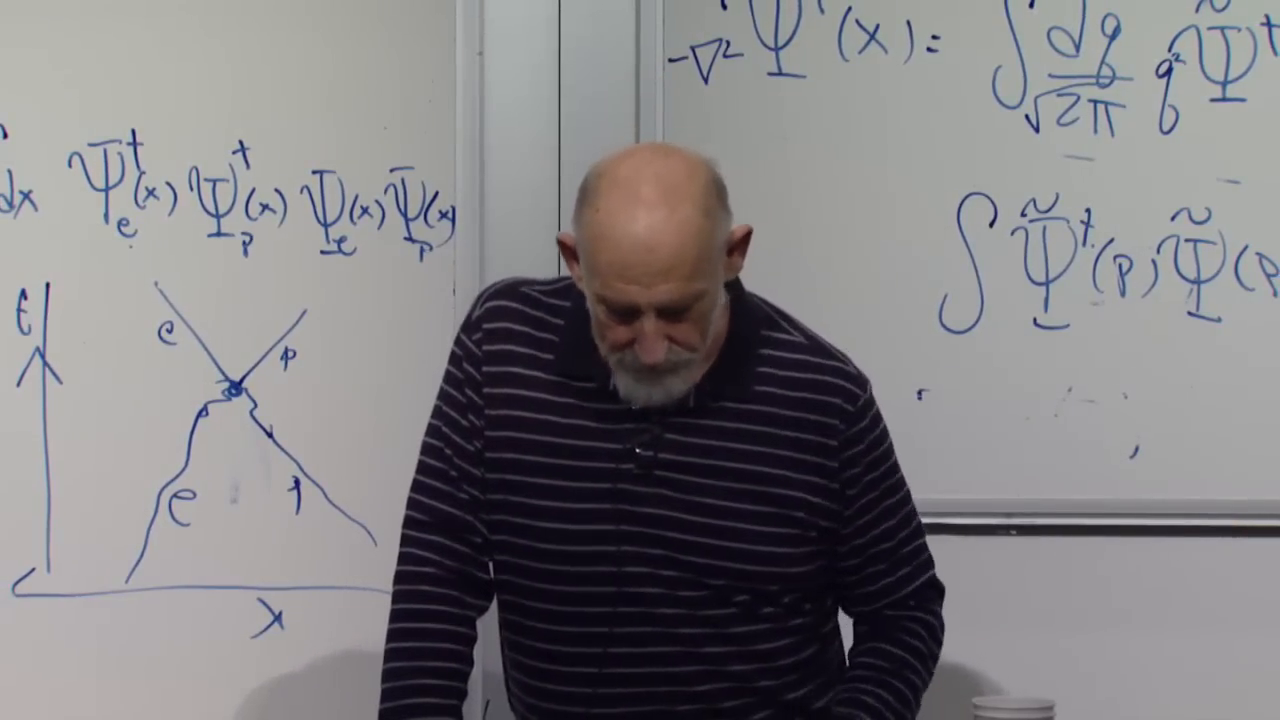
\includegraphics[width=0.94\linewidth]{lecture_09_frame_02.png}\caption{Tương tác tiếp xúc trên bảng. Bốn toán tử trường cục bộ được viết phía trên hình phác không thời gian; điểm gặp nhau là nơi duy nhất tương tác lý tưởng hóa này tác dụng.}\lectureframe{00:35:36}\end{figure}

\begin{figure}[htbp]\centering
\begin{tikzpicture}[x=1.2cm,y=1.0cm,>=Latex]
\draw[->] (-3.0,0) -- (3.0,0) node[right] {$x$};
\draw[->] (0,-0.2) -- (0,4.2) node[above] {$t$};
\coordinate (v) at (0,2.0);
\fill (v) circle (1.8pt);
\draw[thick,->] (-2.2,0.4) -- (v);
\draw[thick,->] (2.0,0.4) -- (v);
\draw[thick,->] (v) -- (-1.6,3.7);
\draw[thick,->] (v) -- (2.2,3.7);
\node[left] at (-1.65,0.7) {$e$};
\node[right] at (1.55,0.7) {$p$};
\node[left] at (-1.15,3.3) {$e$};
\node[right] at (1.65,3.3) {$p$};
\node[right] at (0.12,2.05) {$g$};
\end{tikzpicture}\caption{Bản dựng lại rõ ràng hình ảnh tán xạ cục bộ. Đỉnh là cách viết tắt cho toán tử trong Phương trình~\eqref{eq:l9-contact}, chứ không phải định luật va chạm cổ điển.}\end{figure}

Electron và proton thực tương tác từ xa thông qua thế Coulomb. Mô hình tiếp xúc chỉ là bước đầu ngắn gọn: nếu thực nghiệm cho thấy hai loài hạt chỉ tán xạ khi chúng chồng lấp, thì Phương trình~\eqref{eq:l9-contact} là dạng số hạng ta sẽ đưa vào Hamiltonian.

\begin{classroomqa}\lecturetimestamp{00:35:40}\audiencequestion{Vì sao toán tử tán xạ này lại nằm trong Hamiltonian nếu năng lượng không thay đổi?}\lecturerresponse{Hamiltonian vừa là toán tử năng lượng, vừa là toán tử sinh ra sự biến đổi của trạng thái. Thế năng giữa hai hạt gây ra tán xạ trong quá trình tiến hóa theo thời gian. Bảo toàn năng lượng toàn phần không có nghĩa là trạng thái, hay động lượng riêng lẻ của các hạt, không đổi.}\end{classroomqa}

Điều này cho ta một quy tắc thực hành. Trước hết, hãy tìm hiểu từ thực nghiệm những quá trình cục bộ mà các hạt có thể trải qua. Sau đó, mã hóa các quá trình ấy trong toán tử cập nhật trạng thái. Tích các trường không phải là phép biến đổi đại số để trang trí: các thừa số có dấu dagơ và không có dấu dagơ chỉ rõ loài hạt nào xuất hiện và biến mất.

\section{Phân rã, quá trình nghịch đảo và tính Hermite}

Giả sử buồng bọt cho thấy một vệt của loài \(A\) kết thúc tại một điểm, từ đó xuất hiện các vệt \(B\) và \(C\). Quá trình cục bộ là
\begin{equation}
A\longrightarrow B+C.
\end{equation}
Toán tử thực hiện quá trình đó là
\begin{equation}
V=g\int dx\,
\psi_B^\dagger(x)\psi_C^\dagger(x)\psi_A(x).
\label{eq:l9-decay-half}
\end{equation}
Trường hủy loại bỏ \(A\); hai trường tạo sinh ra \(B\) và \(C\) tại cùng một điểm. Tích phân với trọng số bằng nhau trên mọi \(x\) biểu thị tính bất biến tịnh tiến không gian và lập tức cho
\begin{equation}
p_A=p_B+p_C.
\end{equation}

Hamiltonian phải là toán tử Hermite. Điều này khiến \(e^{-itH}\) là toán tử đơn nhất và bảo toàn xác suất toàn phần. Phương trình~\eqref{eq:l9-decay-half} tự nó không phải Hermite, nên ta phải thêm toán tử liên hợp của nó:
\begin{equation}
H_{\mathrm{int}}
=\int dx\left[
g\,\psi_B^\dagger\psi_C^\dagger\psi_A
+g^*\,\psi_A^\dagger\psi_C\psi_B
\right](x).
\label{eq:l9-hermitian-vertex}
\end{equation}
Với hằng số tương tác thực \(g\), hai hệ số bằng nhau. Liên hợp Hermite đảo thứ tự toán tử, đồng thời hoán đổi các trường có dấu dagơ và không có dấu dagơ. Trong mô hình đồ chơi boson này, các trường thuộc những loài khác nhau giao hoán, nên việc đảo thứ tự không gây thêm phức tạp nào.

Số hạng thứ hai thực hiện quá trình nghịch đảo,
\begin{equation}
B+C\longrightarrow A.
\end{equation}
Vì thế, Hamiltonian kín và đơn nhất cho phép phân rã cũng chứa biên độ tái hợp. Điều đó không bảo đảm cả hai chiều đều xảy ra với mọi tập động lượng ngoài được chọn; các định luật bảo toàn năng lượng và những định luật khác có thể khiến một chiều không thể xảy ra về mặt động học. Điều đó có nghĩa là cả toán tử tương tác lẫn toán tử liên hợp của nó đều thuộc về động lực học.

\begin{classroomqa}\lecturetimestamp{00:42:48}\audiencequestion{Có ngoại lệ nào cho quy tắc rằng quá trình nghịch đảo cũng được phép xảy ra không?}\lecturerresponse{Không, nếu xét ở cấp Hamiltonian của một hệ kín Hermite: tương tác liên hợp là bắt buộc. Một phản ứng ngược cụ thể vẫn có thể bị cấm bởi động học hoặc một số lượng tử được bảo toàn khác, nhưng phần tử ma trận liên hợp vẫn hiện diện.}\end{classroomqa}

Số \(g\) là hằng số tương tác. Nếu \(g\) nhỏ, các hạt gặp nhau sẽ tương tác yếu; nếu nó lớn, biên độ chuyển tiếp lớn hơn. Các hằng số tương tác thường là những tham số được đo trong thực nghiệm, dù các đối xứng có thể liên hệ một số hằng số tưởng như khác nhau.

Cùng quy tắc biểu đạt này cũng mô tả được những phản ứng phức tạp hơn. Trong phân rã beta,
\begin{equation}
n\longrightarrow p+e^-+\bar\nu_e,
\end{equation}
một số hạng cục bộ sơ đồ chứa bốn trường: một trường hủy neutron, ba trường tạo proton, electron và phản neutrino electron, cùng với quá trình liên hợp Hermite. Chỉ vậy cũng đủ để thấy một tập nhỏ các đơn thức toán tử bắt đầu định hình một lý thuyết trường lượng tử như thế nào.

\section{Vì sao bình phương Hamiltonian lại quan trọng}

Công thức thời gian ngắn \eqref{eq:l9-short-update} chỉ giữ lại bậc nhất theo \(\epsilon\). Khai triển đầy đủ là
\begin{equation}
e^{-i\epsilon H}
=1-i\epsilon H-\frac{\epsilon^2}{2}H^2
+\frac{i\epsilon^3}{3!}H^3+\cdots.
\label{eq:l9-exponential}
\end{equation}
Ở bậc hai, Hamiltonian tác dụng hai lần. Đây là nguồn gốc đại số của những hình ảnh quá trình tổ hợp đầu tiên.

Với đỉnh \(A\leftrightarrow B+C\), một lần tác dụng có thể kết hợp \(B+C\) thành \(A\), còn lần thứ hai có thể phân rã \(A\) đó trở lại thành \(B+C\):
\begin{equation}
B+C\longrightarrow A\longrightarrow B+C.
\label{eq:l9-bc-scattering}
\end{equation}
Đóng góp thuần là một biên độ tán xạ \(B+C\to B+C\). Trạng thái trung gian \(A\) không phải là một sự kiện quan sát được bổ sung; nó chỉ trạng thái được lấy tổng qua giữa hai lần tương tác tác dụng.

\begin{classroomqa}\lecturetimestamp{00:49:54}\audiencequestion{Trường \(C\) trong tích toán tử bậc hai được viết trên bảng có cần mang dấu dagơ không?}\lecturerresponse{Có, thứ tự toán tử phải khớp với trình tự đã nêu. Đỉnh thứ nhất hủy \(B\) và \(C\), đồng thời tạo \(A\); đỉnh thứ hai hủy \(A\) rồi tạo lại \(B\) và \(C\). Viết đúng các dấu dagơ tương ứng sẽ khôi phục cách diễn giải ấy.}\end{classroomqa}

\begin{figure}[htbp]\centering
\includegraphics[width=0.94\linewidth]{lecture_09_frame_05.png}\caption{Hai chiều của đỉnh cơ bản \(A\leftrightarrow B+C\) trên bảng. Đặt chúng cạnh nhau là cách biểu diễn trực quan tắt gọn cho quá trình bậc hai trong Phương trình~\eqref{eq:l9-bc-scattering}.}\lectureframe{00:48:56}\end{figure}

Giờ thêm một hạt \(B\) làm nhân chứng. Một lần tương tác cho phép \(A\) phát ra \(C\) và biến thành \(B\); lần tương tác sau cho phép \(C\) ấy kết hợp với \(B\) ban đầu để tạo thành \(A\). Các hạt ngoài vẫn là \(A+B\), nhưng động lượng của chúng có thể thay đổi. Ta mô tả đây là tán xạ \(A\) và \(B\) thông qua trao đổi \(C\).

\begin{figure}[htbp]\centering
\includegraphics[width=0.94\linewidth]{lecture_09_frame_06.png}\caption{Cách dựng quá trình trao đổi trên bảng. Giản đồ bên phải nối hai đỉnh cơ bản bằng một đường \(C\) nội tại, trong khi các hạt \(A\) và \(B\) bên ngoài tán xạ.}\lectureframe{00:51:22}\end{figure}

\begin{figure}[htbp]\centering
\begin{tikzpicture}[x=1.1cm,y=1cm,>=Latex]
\draw[->] (-3.7,-0.2) -- (-3.7,4.2) node[above] {$t$};
\coordinate (v1) at (-0.9,1.25);
\coordinate (v2) at (0.9,2.95);
\fill (v1) circle (1.7pt);
\fill (v2) circle (1.7pt);
\draw[thick,->] (-2.6,0.2) -- (v1) node[midway,below left] {$A$};
\draw[thick,->] (2.6,0.2) -- (v2) node[midway,below right] {$B$};
\draw[thick,->] (v1) -- (-2.4,4.0) node[midway,left] {$B$};
\draw[thick,->] (v2) -- (2.5,4.0) node[midway,right] {$A$};
\draw[thick,->,dashed] (v1) -- (v2) node[midway,above left] {$C$};
\node[below] at (0,-0.05) {$A+B\rightarrow A+B$};
\end{tikzpicture}\caption{Bản dựng lại rõ ràng quá trình trao đổi \(C\). Mỗi chấm đóng góp một thừa số \(g\), nên số hạng bậc hai này tỷ lệ với \(g^2\).}\end{figure}

Mỗi điểm tương tác cục bộ được gọi là một đỉnh. Mỗi đỉnh đóng góp một thừa số bằng hằng số tương tác của nó, vì thế đóng góp có hai đỉnh chứa \(g^2\), đóng góp có ba đỉnh chứa \(g^3\), vân vân. Do đó, một số hạng duy nhất trong Hamiltonian tương quan hóa được cả một họ phản ứng lớn. Đây là một lý do khiến lý thuyết trường lượng tử mạnh mẽ đến vậy: một số ít tương tác cục bộ có thể sắp xếp một lượng dữ liệu tán xạ khổng lồ.

\begin{classroomqa}\lecturetimestamp{00:53:14}\audiencequestion{Quá trình \(A\to B+C\to A\) được gọi là gì?}\lecturerresponse{Đó là một đóng góp tự năng. Một \(A\) được đo không chỉ là trạng thái cơ sở một hạt trần; trạng thái tương tác còn có biên độ cho các thành phần \(B+C\) lân cận. Tán xạ với trạng thái ấy có thể cho thấy cấu trúc đã được bao quanh đó.}\end{classroomqa}

Điện động lực học lượng tử đưa ra ví dụ quen thuộc. Một đỉnh electron--photon cục bộ có thể hủy một electron, tạo lại một electron và tạo ra một photon. Ở bậc hai, electron có thể phát ra rồi tái hấp thụ một photon. Ta dễ bị cám dỗ kể lại điều này như một đoạn phim tí hon, nhưng ý nghĩa chặt chẽ của nó chỉ là một số hạng trong khai triển nhiễu loạn. Electron vật lý là một trạng thái đã được bao quanh, có các thành phần chứa photon.

Ước lượng trong lớp học rằng thành phần này là ``khoảng một phần trăm'' cho thấy quy mô do hằng số cấu trúc tinh tế quyết định, \(\alpha_{\mathrm{em}}\simeq 1/137\). Xác suất chính xác cho một thành phần Fock chứa photon phụ thuộc vào độ phân giải năng lượng và cách định nghĩa trạng thái tương tác; đó không phải là thuộc tính một phần trăm phổ quát của một electron cô lập. Phát biểu vững chắc là tương tác làm thay đổi cấu trúc đo được của electron.

\section{Giản đồ cho biết điều gì và không cho biết điều gì}

Các giản đồ là cách viết tắt phục vụ tính toán cho các lũy thừa của Hamiltonian tương tác. Chúng không phải những diễn biến cổ điển đáng tin cậy, trong đó một hạt chắc chắn thực hiện sự kiện này rồi đến sự kiện khác. Việc nhìn vào bên trong để quyết định phương án trung gian nào đã ``thực sự xảy ra'' sẽ làm thay đổi thí nghiệm và phá hủy tổng kết hợp, cũng như trong giao thoa lượng tử thông thường.

\begin{classroomqa}\lecturetimestamp{00:56:52}\audiencequestion{Tại đỉnh đầu tiên, cả năng lượng lẫn động lượng có được bảo toàn không?}\lecturerresponse{Trong cách xây dựng Hamiltonian tại thời điểm bằng nhau được thực hiện ở đây, tích phân không gian lập tức tạo ra một hàm delta động lượng. Tích phân theo thời gian chưa tạo ra hàm delta năng lượng cho phép chèn riêng lẻ đó. Biên độ tán xạ đầy đủ bất biến tịnh tiến theo thời gian bảo toàn năng lượng toàn phần, còn các đường nội tại không nhất thiết tuân theo hệ thức trên vỏ của các hạt quan sát được. Trong ngôn ngữ giản đồ hiệp biến, bốn động lượng được bảo toàn tại mỗi đỉnh, nhưng các hạt nội tại có thể nằm ngoài vỏ.}\end{classroomqa}

Năng lượng dường như bị thiếu trong hình dung ngây thơ về một đỉnh là lời nhắc khác rằng không được bỏ qua năng lượng tương tác. Hamiltonian toàn phần không chỉ là tổng năng lượng của các hạt tự do. Nếu thấy khó hiểu, hãy quay lại Phương trình~\eqref{eq:l9-exponential}: hình vẽ biểu diễn một số hạng trong khai triển tiến hóa đơn nhất theo thời gian. Công cụ giản đồ Feynman đầy đủ cung cấp cách sắp thứ tự thời gian, các hàm truyền, phép tích phân và các hệ số đối xứng một cách có hệ thống, nhưng vật lý cơ bản bắt đầu từ đây.

Một câu hỏi mở rộng diễn giải giản đồ quá sát nghĩa khi so sánh photon phát ra với điện trường bao quanh một electron chuyển động chậm.

\begin{classroomqa}\lecturetimestamp{00:58:26}\audiencequestion{Điện trường của electron ở khoảng cách xa có thực sự do các photon bức xạ tạo ra không? Điều đó liên hệ thế nào với giao thoa và hiệu ứng Aharon--Bohm?}\lecturerresponse{Trường tĩnh hoặc trường cảm ứng không phải là dòng photon bức xạ thực. Điện động lực học lượng tử mô tả cả bức xạ lẫn sự bao quanh điện từ của electron bằng cùng một trường, nhưng các trạng thái lượng tử và động học tương ứng khác nhau. Với electron siêu tương đối tính, một số thành phần trường có thể được xem hữu ích như một dòng photon gần thực; với electron chậm, hình dung quỹ đạo photon theo nghĩa đen là không phù hợp. Giao thoa hai khe và hiệu ứng Aharon--Bohm cũng là những hiện tượng trường phi cổ điển, nhưng chúng không biến giản đồ tự năng này thành một đoạn phim cơ học.}\end{classroomqa}

\begin{classroomqa}\lecturetimestamp{01:01:28}\audiencequestion{Chính xác thì vì sao mô hình cổ điển của giản đồ lại thất bại?}\lecturerresponse{Vì phép tính cộng kết hợp các biên độ của mọi phương án trung gian được phép. Kinh nghiệm khiến các hình vẽ trở nên trực quan, nhưng ý nghĩa theo nghĩa đen của chúng không bao giờ vượt quá khai triển toán tử định nghĩa chúng. Chúng là cách tính gọn cho \(H^2,H^3,\ldots\), chứ không phải bản ghi những sự kiện trung gian đã được quan sát.}\end{classroomqa}

\begin{classroomqa}\lecturetimestamp{01:03:04}\audiencequestion{Tương tác Coulomb thông thường có thể xuất hiện như giới hạn cổ điển của quá trình trao đổi photon không?}\lecturerresponse{Có. Tính biên độ thích hợp do photon trung gian và lấy giới hạn tĩnh phi tương đối tính sẽ cho thế Coulomb. Phép suy dẫn này phức tạp hơn phần phác họa toán tử ở đây, và cũng không nên được hiểu là photon thực sự nhảy giữa hai hạt cổ điển.}\end{classroomqa}

\begin{classroomqa}\lecturetimestamp{01:03:44}\audiencequestion{Các hằng số tương tác có được tính từ tích các trường không?}\lecturerresponse{Thông thường, giá trị số của chúng là dữ liệu đầu vào từ thực nghiệm. Đối xứng có thể ràng buộc chúng hoặc liên hệ các hằng số vốn dĩ sẽ độc lập. Khi một quan hệ như vậy dự đoán độ mạnh tương đối của những phản ứng khác nhau và thực nghiệm xác nhận điều đó, sự phù hợp đặc biệt có ý nghĩa.}\end{classroomqa}

\begin{classroomqa}\lecturetimestamp{01:04:48}\audiencequestion{Đối xứng ngẫu nhiên khác đối xứng chuẩn tắc như thế nào về vai trò?}\lecturerresponse{Đối xứng chuẩn tắc trực tiếp ràng buộc cấu trúc được phép và các quan hệ giữa những hằng số tương tác. Đối xứng ngẫu nhiên không được áp đặt ở cấp cơ bản, mà xuất hiện vì mọi tương tác được phép ở bậc thấp hơn tình cờ đều tôn trọng nó. Đối xứng ấy vẫn có thể dẫn đến những hệ quả quan trọng, dù nguồn gốc và độ bền vững khác với đối xứng chuẩn tắc.}\end{classroomqa}

Tạm thời, thế là đủ về lý thuyết trường phi tương đối tính. Ta đã hứa sẽ nói về fermion. Thay vì lượng tử hóa lần hai chúng ngay lập tức, trước hết ta sẽ tìm hiểu phương trình một hạt tương đối tính mà các toán tử trường của chúng phải thỏa mãn.

\section{Vì sao electron cần đến thuyết tương đối}

Bắt đầu với một chiều không gian. Đây không phải là hạn chế thực tế, nhưng nó loại bỏ sự phức tạp hình học của spin trong ba chiều mà vẫn giữ nguyên phần đại số cốt yếu. Electron đủ nhẹ để hiệu ứng tương đối tính quan trọng ngay cả trong nguyên tử. Trong nguyên tử hydro, tốc độ đặc trưng của nó cỡ
\begin{equation}
v\sim\alpha_{\mathrm{em}}c\approx 0.007c,
\end{equation}
xấp xỉ một phần trăm tốc độ ánh sáng. Với các electron lớp trong của nguyên tử nặng, thang ước lượng trở thành \(v\sim Z\alpha_{\mathrm{em}}c\), nên hiệu chỉnh tương đối tính có thể đáng kể. Dù động lực quyết định là sự tò mò lịch sử hay độ chính xác trong vật lý nguyên tử, một phương trình kiểu Schr\"odinger tương đối tính vẫn cần thiết về mặt vật lý.

Cách lượng tử hóa thông thường bắt đầu từ hệ thức cổ điển giữa năng lượng và động lượng. Trong giới hạn phi tương đối tính,
\begin{equation}
E=\frac{p^2}{2m},
\end{equation}
và các phép thay thế
\begin{equation}
E\mapsto i\partial_t,
\qquad
p\mapsto-i\partial_x
\end{equation}
cho
\begin{equation}
i\partial_t\varphi(x,t)
=-\frac{1}{2m}\partial_x^2\varphi(x,t).
\end{equation}

Thuyết tương đối thay vào đó cho hệ thức, với \(c=1\),
\begin{equation}
E^2=p^2+m^2.
\label{eq:l9-rel-dispersion}
\end{equation}

\begin{figure}[htbp]\centering
\includegraphics[width=0.94\linewidth]{lecture_09_frame_07.png}\caption{Bước chuyển trên bảng từ \(E=p^2/2m\) sang hệ thức tương đối tính \(E^2=p^2+m^2\), với \(c=1\).}\lectureframe{01:10:30}\end{figure}

Áp dụng các phép thay thế vào hệ thức bình phương cho
\begin{equation}
-\partial_t^2\varphi
=\left(-\partial_x^2+m^2\right)\varphi,
\label{eq:l9-klein-gordon}
\end{equation}
hoặc tương đương
\begin{equation}
\left(\partial_t^2-\partial_x^2+m^2\right)\varphi=0.
\end{equation}
Đây là phương trình Klein--Gordon. Đây là một phương trình trường tương đối tính hoàn toàn có ý nghĩa, đặc biệt đối với các trường spin không. Nhưng phương trình electron ta cần phải bậc nhất theo thời gian,
\begin{equation}
i\partial_t\Psi=H\Psi,
\end{equation}
để chính \(H\), chứ không chỉ \(H^2\), sinh ra sự tiến hóa.

Về hình thức, ta có thể chọn
\begin{equation}
H=\sqrt{-\partial_x^2+m^2}.
\end{equation}
Căn bậc hai có thể được định nghĩa rõ ràng trong không gian động lượng, nơi nó nhân với \(\sqrt{p^2+m^2}\), nhưng trong không gian vị trí, nó là một toán tử giả vi phân phi cục bộ. Toán tử này có ý nghĩa kỹ thuật, nhưng không hữu ích về mặt thẩm mỹ cho phương trình cục bộ mà ta đang tìm. Vì vậy, ta bắt đầu lại.

\section{Sóng không khối lượng chuyển động sang phải}

Trước hết, xét một hạt không khối lượng chuyển động sang phải. Năng lượng dương và động lượng của nó thỏa mãn
\begin{equation}
E=p
\qquad (c=1).
\end{equation}
Lượng tử hóa cho
\begin{equation}
i\partial_t\psi=-i\partial_x\psi,
\end{equation}
hoặc
\begin{equation}
(\partial_t+\partial_x)\psi=0.
\label{eq:l9-right-mover}
\end{equation}
Mọi nghiệm đều có dạng
\begin{equation}
\psi(x,t)=f(x-t).
\end{equation}
Dạng sóng giữ nguyên hình dạng và chuyển động sang phải với tốc độ ánh sáng.

Hai khó khăn xuất hiện ngay lập tức. Thứ nhất, nếu cho phép Phương trình~\eqref{eq:l9-right-mover} tác dụng lên các mode Fourier tùy ý, động lượng âm có năng lượng \(E=p<0\), nên Hamiltonian không bị chặn dưới. Nếu tự áp đặt điều kiện \(p>0\), ta chỉ giữ lại các sóng chuyển động sang phải, và đó vẫn chưa phải lý thuyết electron mà ta cần. Thứ hai, phương trình này chỉ cho phép chuyển động theo một chiều: nó không chứa electron thông thường chuyển động sang trái. Trước hết, ta sẽ giải quyết vấn đề trái-phải, còn để nguyên các năng lượng âm.

\section{Hai thành phần và ma trận alpha}

Đưa vào hai biên độ,
\begin{equation}
\Psi(x,t)=
\begin{pmatrix}
\psi_1(x,t)\\[3pt]
\psi_2(x,t)
\end{pmatrix},
\end{equation}
trong đó \(\psi_1\) chuyển động sang phải và \(\psi_2\) chuyển động sang trái trong giới hạn không khối lượng:
\begin{align}
(\partial_t+\partial_x)\psi_1&=0,
&
(\partial_t-\partial_x)\psi_2&=0.
\end{align}
Cơ học lượng tử cũng cho phép chồng chập tùy ý của hai thành phần này. Vì vậy, một hạt có thể có biên độ ứng với cả hai hướng, thay vì mang một nhãn cổ điển được chọn một lần rồi giữ nguyên.

Bậc tự do hai trị bổ sung này giống spin về mặt đại số, nhưng trong một chiều nó không phải là mômen động lượng thông thường. Định nghĩa
\begin{equation}
\alpha=
\begin{pmatrix}
1&0\\
0&-1
\end{pmatrix}
=\sigma_3.
\label{eq:l9-alpha}
\end{equation}
Các vectơ riêng ứng với trị riêng \(+1\) của nó chọn thành phần truyền sang phải, còn các vectơ riêng ứng với trị riêng \(-1\) chọn thành phần truyền sang trái. Trong lý thuyết không khối lượng, Hamiltonian có dạng đơn giản
\begin{equation}
H=\alpha p,
\end{equation}
và hai phương trình hợp thành
\begin{equation}
i\partial_t\Psi=-i\alpha\partial_x\Psi.
\label{eq:l9-massless-dirac}
\end{equation}

\begin{classroomqa}
\lecturetimestamp{01:22:44}
\audiencequestion{Ma trận đường chéo phân biệt hai thành phần có tên gọi là gì?}
\lecturerresponse{Nếu xét như một ma trận Pauli, đó là \(\sigma_3\), chứ không phải \(\sigma_1\). Trong ký hiệu Dirac dùng cho cấu trúc đang xét, ta gọi nó là \(\alpha\). Đại số của nó chính là đại số Pauli quen thuộc, dù ở đây nhãn vật lý là chiều truyền chứ không phải mômen động lượng spin.}
\end{classroomqa}

\begin{classroomqa}
\lecturetimestamp{01:23:32}
\audiencequestion{Trong ba chiều, khi hướng là một vectơ, cấu trúc này có ý nghĩa hình học rõ hơn không?}
\lecturerresponse{Có. Bài toán ba chiều cần một ma trận cho mỗi phương không gian và dẫn đến cấu trúc spinor phong phú hơn. Dù vậy, mô hình một chiều vẫn chính xác trong phạm vi của nó và tách riêng đại số trái-phải cốt yếu mà không có phần phức tạp bổ sung đó.}
\end{classroomqa}

\begin{figure}[htbp]
\centering
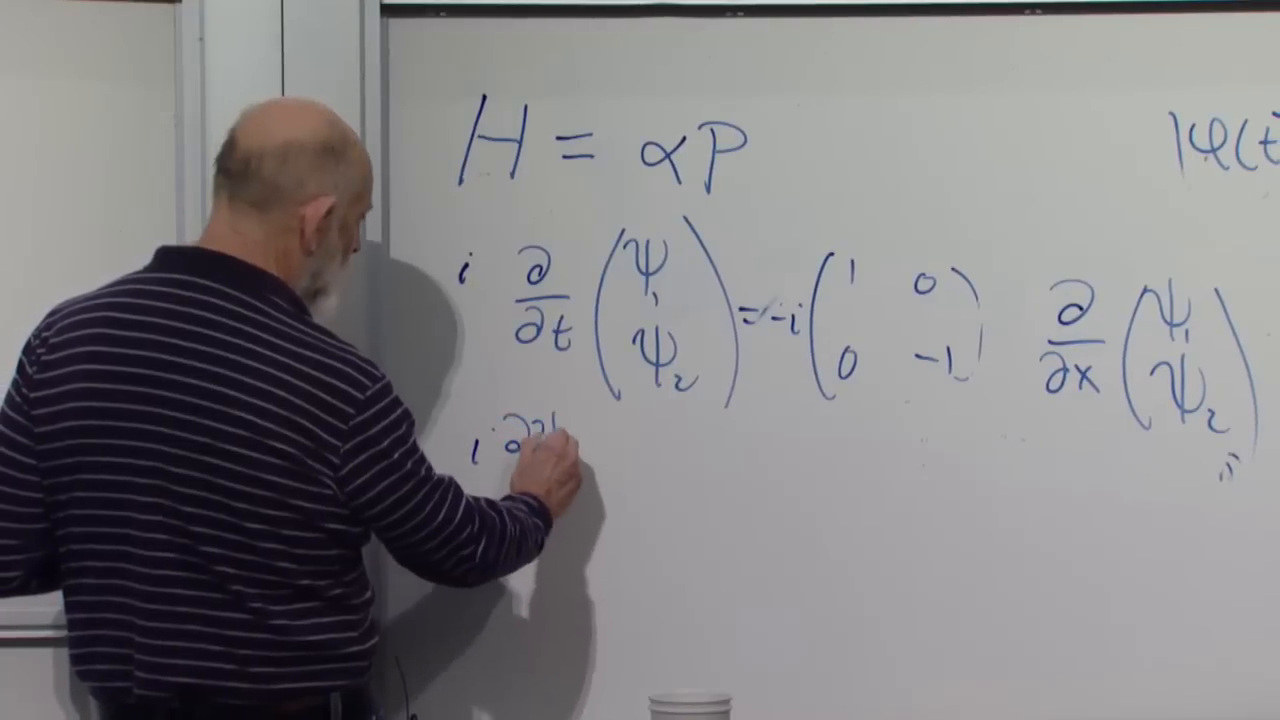
\includegraphics[width=0.94\linewidth]{lecture_09_frame_03.png}
\caption{Phương trình hai thành phần không khối lượng trên bảng: \(H=\alpha P\), trong đó ma trận đường chéo gán chiều truyền ngược nhau cho \(\psi_1\) và \(\psi_2\).}
\lectureframe{01:26:00}
\end{figure}

Bài toán chỉ có một chiều truyền đã được giải quyết. Phổ năng lượng âm vẫn còn đó, và ta phát hiện ra khiếm khuyết thứ ba: hai thành phần vẫn không có khối lượng và truyền đi với tốc độ ánh sáng. Bước tiếp theo phải đưa năng lượng nghỉ vào và ghép hai chiều truyền với nhau.

\section{Thêm khối lượng và khám phá đại số Dirac}

Thêm số hạng đơn giản tổng quát nhất tỉ lệ với khối lượng,
\begin{equation}
H=\alpha p+\beta m,
\label{eq:l9-dirac-hamiltonian}
\end{equation}
trong đó \(\beta\) chỉ tác động lên chỉ số hai thành phần. Số hạng này có thể là ma trận đơn vị hoặc một ma trận khác; ta để hệ thức tán sắc tương đối tính quyết định.

Vì \(H^2\) phải bằng \(p^2+m^2\), hãy bình phương phương trình ~\eqref{eq:l9-dirac-hamiltonian}:
\begin{align}
H^2
&=(\alpha p+\beta m)^2\\
&=\alpha^2p^2+\beta^2m^2
+(\alpha\beta+\beta\alpha)pm.
\label{eq:l9-square-dirac}
\end{align}
Các ma trận giao hoán với \(p\) vì chúng tác động lên không gian nội tại hai thành phần, còn \(p\) tác động lên hàm sóng không gian. Để khớp với phương trình ~\eqref{eq:l9-rel-dispersion}, cần có
\begin{equation}
\alpha^2=\mathbb{1},
\qquad
\beta^2=\mathbb{1},
\qquad
\{\alpha,\beta\}
=\alpha\beta+\beta\alpha=0.
\label{eq:l9-dirac-algebra}
\end{equation}
Điều kiện thứ nhất đã được thỏa mãn với \(\alpha=\sigma_3\). Mọi ma trận Pauli khác đều phản giao hoán với nó và bình phương thành ma trận đơn vị. Chọn
\begin{equation}
\beta=
\begin{pmatrix}
0&1\\
1&0
\end{pmatrix}
=\sigma_1.
\label{eq:l9-beta}
\end{equation}
Việc chọn \(\sigma_1\) thay vì \(\sigma_2\) chỉ là quy ước cơ sở; cả hai đều hiện thực hóa cùng một đại số sau một phép đổi cơ sở unita.

\begin{classroomqa}
\lecturetimestamp{01:33:00}
\audiencequestion{Dirac có đơn giản là nhận ra các ma trận Pauli thỏa mãn những điều kiện đại số này không?}
\lecturerresponse{Phép suy dẫn trong lịch sử được thực hiện trực tiếp trong ba chiều và đưa vào các ma trận thỏa mãn những hệ thức cần thiết. Khi đã viết ra các điều kiện, đại số Pauli cho thấy ngay nghiệm một chiều: chọn hai ma trận Pauli khác nhau.}
\end{classroomqa}

\begin{classroomqa}
\lecturetimestamp{01:34:24}
\audiencequestion{Đây có phải là tham số vận tốc tương đối tính \(\beta\) không?\(v/c\)}
\lecturerresponse{Không. Đây là một ma trận tác động lên các thành phần spinor. Chữ cái được dùng lại chỉ là ký hiệu của Dirac; nó không liên quan gì đến đại lượng động học \(v/c\).}
\end{classroomqa}

Trong ba chiều không gian, các ma trận \(2\times2\) là không đủ để tạo thành tập đầy đủ các ma trận phản giao hoán cần thiết. Ta sẽ xét việc mở rộng đó sau. Trong một chiều, các phương trình ~\eqref{eq:l9-alpha} và \eqref{eq:l9-beta} là đủ.

\section{Phương trình Dirac một chiều có ghép nối}

Thay \(p=-i\partial_x\) vào, ta thu được phương trình Dirac một chiều ở dạng Hamiltonian:
\begin{equation}
i\partial_t\Psi
=\left(-i\alpha\partial_x+\beta m\right)\Psi.
\label{eq:l9-one-dimensional-dirac}
\end{equation}
Vì \(\alpha\) là ma trận đường chéo nên số hạng đạo hàm giữ hai thành phần tách biệt. Vì \(\beta\) là ma trận ngoài đường chéo nên số hạng khối lượng hoán đổi chúng cho nhau. Viết riêng từng thành phần,
\begin{align}
i\partial_t\psi_1
&=-i\partial_x\psi_1+m\psi_2,
\label{eq:l9-dirac-component-one}\\
i\partial_t\psi_2
&=+i\partial_x\psi_2+m\psi_1.
\label{eq:l9-dirac-component-two}
\end{align}

\begin{figure}[htbp]
\centering
\includegraphics[width=0.94\linewidth]{lecture_09_frame_08.png}
\caption{Các phương trình thành phần có ghép nối trên bảng. Dấu đạo hàm trái ngược nhau biểu thị chuyển động sang phải và sang trái; số hạng khối lượng ngoài đường chéo hoán đổi \(\psi_1\) và \(\psi_2\).}
\lectureframe{01:37:44}
\end{figure}

Các thành phần không còn tiến hóa độc lập ngay khi \(m\ne0\). Bình phương phương trình bậc nhất thu lại toán tử Klein--Gordon trên mỗi thành phần,
\begin{equation}
\left(\partial_t^2-\partial_x^2+m^2\right)\psi_a=0,
\qquad a=1,2,
\end{equation}
và sóng phẳng thỏa mãn \(E^2=p^2+m^2\). Vận tốc nhóm của chúng là
\begin{equation}
v_g=\frac{dE}{dp}=\frac{p}{E},
\end{equation}
độ lớn của vận tốc này nhỏ hơn một khi khối lượng khác không.

Mối liên hệ giữa khối lượng và sự trộn lẫn trái-phải không phải là ngẫu nhiên. Một hạt chuyển động sang phải không khối lượng vẫn chuyển động sang phải dưới mọi phép biến đổi Lorentz chính tắc; không người quan sát nào chuyển động dưới ánh sáng có thể vượt qua ánh sáng rồi đảo chiều truyền của nó. Một hạt có khối lượng có thể được đưa về trạng thái nghỉ, rồi được quan sát từ một hệ quy chiếu chuyển động nhanh hơn theo cùng chiều, trong đó vận tốc của nó có vẻ như đã đảo chiều. Vì vậy, lý thuyết tương đối tính có khối lượng không thể giữ các khu vực trái và phải tách biệt vĩnh viễn. Số hạng khối lượng ngoài đường chéo tạo ra chính xác sự ghép nối cần thiết.

\begin{classroomqa}
\lecturetimestamp{01:40:01}
\audiencequestion{Sự hoán đổi hai thành phần có phải là dao động chiral không?}
\lecturerresponse{Trong cơ sở một chiều này, \(\alpha\) phân biệt hai chiều chiral không khối lượng. Số hạng khối lượng nằm ngoài đường chéo và trộn lẫn chúng, vì thế tính chiral không còn được bảo toàn. Theo nghĩa đó, số hạng khối lượng là nguồn gốc của dao động chiral.}
\end{classroomqa}

\begin{classroomqa}
\lecturetimestamp{01:40:46}
\audiencequestion{Vì sao phương trình của fermion lại phải là căn bậc hai của phương trình boson?}
\lecturerresponse{Không nên hiểu vấn đề theo cách đó. Hệ thức tán sắc \(E^2=p^2+m^2\) áp dụng cho mọi hạt tương đối tính tự do, bất kể thống kê. Toán tử Dirac tình cờ cho ta một phép phân tích nhân tử dạng ma trận của toán tử Klein--Gordon, nhưng quan hệ đại số đó không suy ra fermion từ boson.}
\end{classroomqa}

\begin{classroomqa}
\lecturetimestamp{01:41:31}
\audiencequestion{Có thể phân tích phương trình thành các nhân tử vô hướng đơn giản, tách riêng phần truyền sang trái và sang phải không?}
\lecturerresponse{Chỉ trong giới hạn không khối lượng thì hai phương trình chiral mới tách thành các nhân tử vô hướng độc lập. Khi \(m\ne0\), phép phân tích nhân tử hữu ích có dạng ma trận: chính các ma trận phản giao hoán \(\alpha\) và \(\beta\) loại bỏ số hạng chéo không mong muốn.}
\end{classroomqa}

\begin{classroomqa}
\lecturetimestamp{01:42:04}
\audiencequestion{Hai phương trình có ghép nối này đã cấu thành phương trình Dirac chưa?}
\lecturerresponse{Đúng. Kết hợp lại, chúng là phương trình Dirac trong một chiều không gian, tương đương với dạng gọn ở phương trình ~\eqref{eq:l9-one-dimensional-dirac}. Có thể thu được một ký hiệu hiệp biến đối xứng hơn bằng cách nhân với \(\beta\), nhưng ta sẽ để dạng đó lại phần sau.}
\end{classroomqa}

Cố ý còn để dở hai việc. Cấu trúc này chưa loại bỏ năng lượng âm; nó cung cấp nghiệm năng lượng âm trong cả hai khu vực có hướng truyền, khiến vấn đề ấy trở nên rõ ràng hơn chứ không bớt đi. Và lý thuyết vẫn chỉ tồn tại trong một chiều không gian. Diễn giải các nghiệm năng lượng âm và mở rộng đại số ma trận lên \(3+1\) chiều là những bước tiếp theo.

\chapter{Các fermion, ma trận Dirac và biển Dirac}

Biển Dirac là đích đến của chúng ta, nhưng con đường dẫn tới đó cũng quan trọng. Trước khi xét năng lượng âm trong lý thuyết electron tương đối tính, ta cần hai công cụ. Trước hết là đại số toán tử phân biệt fermion với boson. Tiếp theo là ôn lại phương trình Dirac một chiều, nơi có thể thấy rõ từng bước mở rộng hàm sóng mà không bị vướng vào hình học của ba chiều không gian. Khi đã có những công cụ ấy, phương trình ba chiều sẽ buộc ta phải có một cấu trúc ma trận riêng, và phần mở đầu bàn về các trạng thái fermion đầy và trống sẽ trở lại như chìa khóa để hiểu positron.

Ta dùng \(c=\hbar=1\). Chữ \(P\) viết hoa ký hiệu toán tử động lượng, chữ \(p\) viết thường ký hiệu trị riêng động lượng, còn các ký hiệu in đậm là phiên bản ba chiều của chúng.

\section{Trao đổi được biểu diễn bằng đại số toán tử}

Xét hai hạt giống hệt nhau, một hạt ở \(x\) và hạt kia ở \(y\). Các nhãn \(x\) và \(y\) chỉ các vị trí đầy đủ; chúng không phải là hai tọa độ Descartes của cùng một hạt. Tác dụng hai toán tử tạo lên chân không cho ta
\begin{equation}
\lvert x,y\rangle
=
\psi^\dagger(x)\psi^\dagger(y)\lvert0\rangle.
\label{eq:l10-two-particle-state}
\end{equation}

Đối với boson, đổi chỗ hai vị trí không làm thay đổi trạng thái:
\begin{equation}
\lvert x,y\rangle=\lvert y,x\rangle.
\end{equation}
Phát biểu toán tử bảo đảm tính đối xứng này là
\begin{equation}
\psi^\dagger(x)\psi^\dagger(y)
=
\psi^\dagger(y)\psi^\dagger(x).
\label{eq:l10-boson-exchange}
\end{equation}
Hai toán tử tạo boson giao hoán, nên ta có thể đảo thứ tự của chúng mà không làm thay đổi trạng thái được tạo ra.

Đối với fermion, phép đổi chỗ làm đổi dấu:
\begin{equation}
\lvert x,y\rangle=-\lvert y,x\rangle.
\label{eq:l10-fermion-state-exchange}
\end{equation}
Dấu tổng thể của một vectơ trạng thái riêng lẻ không phải là đại lượng quan sát được, nhưng dấu tương đối giữa các khả năng thì có thể quan sát được, vì vậy phải giữ nhất quán dấu trừ này. Phương trình~\eqref{eq:l10-fermion-state-exchange} đòi hỏi
\begin{equation}
\psi^\dagger(x)\psi^\dagger(y)
=
-\,\psi^\dagger(y)\psi^\dagger(x).
\label{eq:l10-fermion-operator-exchange}
\end{equation}

\begin{figure}[htbp]
\centering
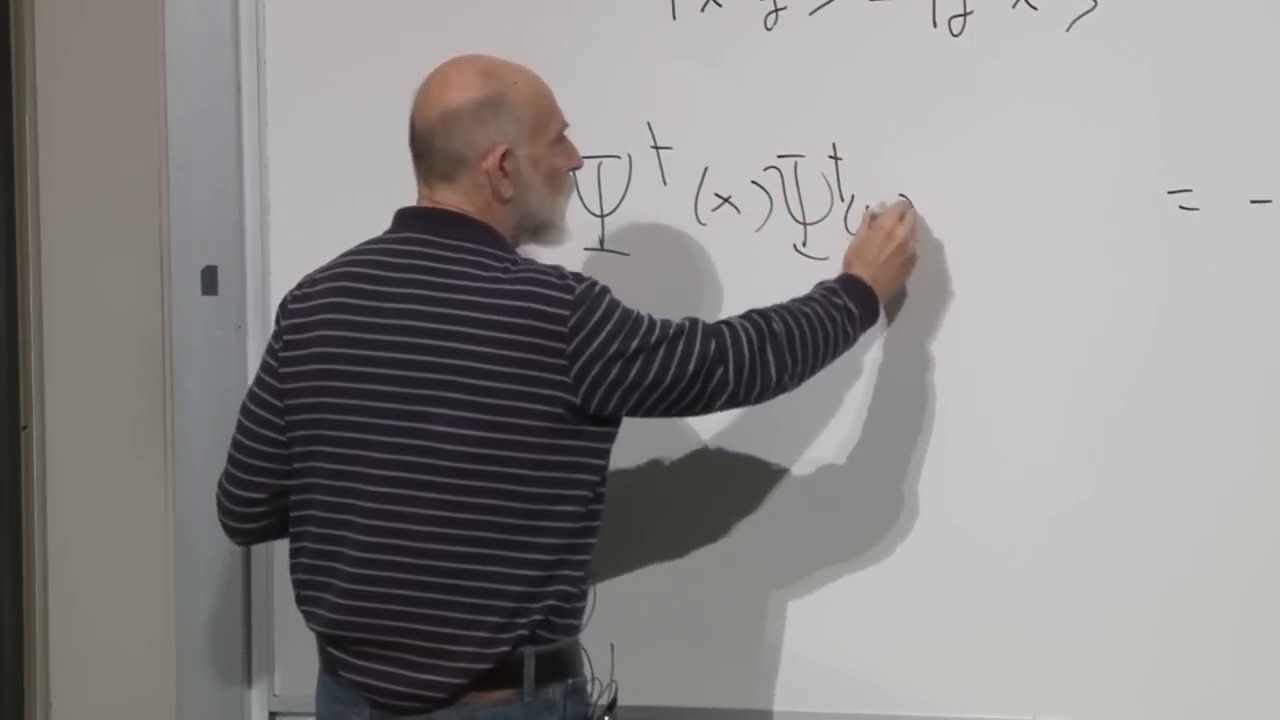
\includegraphics[width=0.94\linewidth]{lecture_10_figure_02.png}
\caption{Quan hệ trên bảng biểu diễn phép trao đổi fermion. Đổi chỗ các toán tử tạo làm đổi dấu trạng thái hai hạt.}
\lectureframe{00:05:50}
\end{figure}

Với hai toán tử bất kỳ \(A\) và \(B\), ta định nghĩa phản giao hoán tử là
\begin{equation}
\{A,B\}:=AB+BA.
\end{equation}
Do đó, quy tắc trao đổi là
\begin{equation}
\{\psi^\dagger(x),\psi^\dagger(y)\}=0.
\label{eq:l10-creation-anticommutator}
\end{equation}
Đại số trường fermion tương ứng thay các giao hoán tử của boson bằng phản giao hoán tử. Cần phân biệt hai cách dùng từ này: các toán tử trường phản giao hoán do thống kê Fermi, còn các ma trận sau này sẽ phản giao hoán để triệt tiêu các số hạng chéo trong hệ thức tán sắc tương đối tính.

Bây giờ đặt \(y=x\) trong Eq.~\eqref{eq:l10-creation-anticommutator}. Hai tích trở thành như nhau:
\begin{align}
0
&=\{\psi^\dagger(x),\psi^\dagger(x)\}\\
&=2\,\psi^\dagger(x)\psi^\dagger(x).
\end{align}
Vậy
\begin{equation}
\bigl(\psi^\dagger(x)\bigr)^2=0.
\label{eq:l10-exclusion}
\end{equation}
Cố tạo hai fermion giống hệt nhau trong cùng một trạng thái một hạt sẽ cho vectơ không. Đó là nguyên lý loại trừ ở dạng toán tử.

\begin{figure}[htbp]
\centering
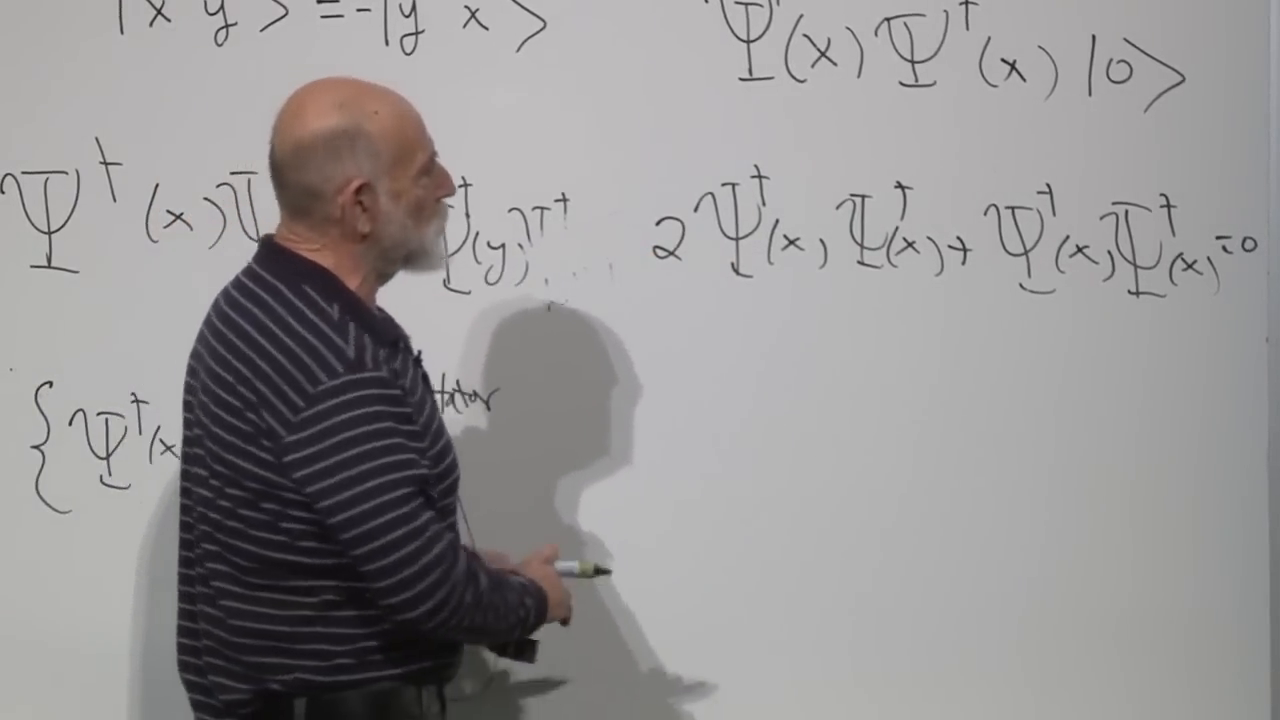
\includegraphics[width=0.94\linewidth]{lecture_10_figure_03.png}
\caption{Trường hợp hai trạng thái bằng nhau trên bảng. Tích lặp của các toán tử tạo xuất hiện hai lần nên phải triệt tiêu.}
\lectureframe{00:08:04}
\end{figure}

\begin{figure}[htbp]
\centering
\begin{adjustbox}{max width=\linewidth}
\begin{tikzpicture}[node distance=1.25cm,>=Latex]
\node[draw,rounded corners,align=center,inner sep=7pt] (a)
  {$\{\psi^\dagger(x),\psi^\dagger(x)\}=0$};
\node[draw,rounded corners,align=center,inner sep=7pt,right=of a] (b)
  {$2(\psi^\dagger(x))^2=0$};
\node[draw,rounded corners,align=center,inner sep=7pt,right=of b] (c)
  {$(\psi^\dagger(x))^2=0$};
\draw[->,thick] (a) -- (b);
\draw[->,thick] (b) -- (c);
\end{tikzpicture}
\end{adjustbox}
\caption{Lập luận về nguyên lý loại trừ được dựng lại đầy đủ, không có phần trung gian trên bảng đã bị xóa dở.}
\end{figure}

\section{Vì sao trạng thái đầy và trống đối xứng với nhau đối với fermion}

Có một khác biệt thứ hai giữa toán tử boson và fermion, tinh tế hơn nguyên lý loại trừ và về sau sẽ rất quan trọng. Với một mode boson,
\begin{equation}
[a,a^\dagger]=1,
\qquad
n=0,1,2,\ldots.
\end{equation}
Đổi thứ tự \(a\) và \(a^\dagger\) làm đổi dấu giao hoán tử. Ngay cả khi chỉ gọi các toán tử là \(A\) và \(B\), đại số vẫn cho ta biết thứ tự nào làm tăng số chiếm và thứ tự nào làm giảm nó.

Thang số chiếm của boson còn có một chiều xác định. Toán tử hủy cuối cùng đi tới \(\lvert0\rangle\) và tác dụng lên đó cho kết quả không, trong khi toán tử tạo có thể tiếp tục mãi:
\begin{align}
a\lvert0\rangle&=0,\\
a^\dagger\lvert n\rangle&\propto\lvert n+1\rangle,
\qquad n=0,1,2,\ldots.
\end{align}
Lật ngược thang này không cho lại cùng một phổ. Thang có đáy nhưng không có đỉnh.

Với một mode fermion,
\begin{equation}
\{a,a^\dagger\}=1,
\qquad
a^2=(a^\dagger)^2=0,
\qquad
n=0,1.
\label{eq:l10-fermion-mode}
\end{equation}
Toán tử tạo đưa trạng thái trống thành trạng thái đầy rồi dừng lại:
\begin{equation}
a^\dagger\lvert0\rangle=\lvert1\rangle,
\qquad
a^\dagger\lvert1\rangle=0.
\end{equation}
Toán tử hủy thực hiện quá trình ngược lại:
\begin{equation}
a\lvert1\rangle=\lvert0\rangle,
\qquad
a\lvert0\rangle=0.
\end{equation}
Chỉ có hai trạng thái, nên sơ đồ đối xứng khi đổi trạng thái đầy với trạng thái trống và đổi \(a\) với \(a^\dagger\). Các toán tử vẫn mang ý nghĩa vật lý khác nhau, nhưng đại số của chúng không còn ưu tiên toán tử này là toán tử tạo và toán tử kia là toán tử hủy. Sự đối xứng hình thức này là mầm mống của cách diễn giải lại theo hạt và lỗ trống.

\begin{classroomqa}
\lecturetimestamp{00:13:54}
\audiencequestion{Nếu \((a^\dagger)^2=0\), điều đó có mâu thuẫn không, hay nó hàm ý rằng \(a^\dagger=0\)?}
\lecturerresponse{Không phải cả hai. Một toán tử khác không có thể có bình phương bằng không. Ở đây, \(a^\dagger\) biến \(\lvert0\rangle\) thành \(\lvert1\rangle\), nhưng không có trạng thái khả dĩ nào phía trên \(\lvert1\rangle\), nên tác dụng toán tử ấy hai lần cho kết quả không. Lập luận tương tự cho ta \(a^2=0\).}
\end{classroomqa}

Hãy tạm ghi nhớ sự đối xứng giữa trạng thái đầy và trống này. Khi một electron năng lượng âm bị lấy đi, toán tử hủy sẽ được đổi tên thành toán tử tạo positron. Đó không phải là thay đổi ký hiệu tùy tiện; phép đổi tên này sử dụng đúng đại số fermion hai trạng thái đã thiết lập ở đây.

\section{Cấu tạo phương trình Dirac một chiều}

Giờ hãy trở lại với một hạt trong một chiều không gian. Phương trình sóng tương đối tính bậc nhất đơn giản nhất là
\begin{equation}
i\partial_t\psi=-\,i\partial_x\psi.
\label{eq:l10-right-mover}
\end{equation}
Với \(P=-i\partial_x\), ta có
\begin{equation}
H=P.
\end{equation}
Trạng thái riêng động lượng có \(E=p\), và vận tốc nhóm của nó là
\begin{equation}
v_g=\frac{dE}{dp}=1.
\end{equation}
Động lượng dương hay âm, và do đó năng lượng dương hay âm, vẫn cho một sóng truyền cứng sang phải. Dấu của \(p\) làm thay đổi dạng pha, chứ không làm đổi hướng truyền.

Một hạt có khối lượng phải có khả năng chuyển động theo cả hai hướng. Đưa vào thành phần thứ hai thỏa mãn
\begin{equation}
H\psi_1=P\psi_1,
\qquad
H\psi_2=-P\psi_2.
\label{eq:l10-two-directions}
\end{equation}
Thành phần thứ nhất truyền sang phải; thành phần thứ hai truyền sang trái. Gom chúng thành một cột,
\begin{equation}
\Psi=
\begin{pmatrix}
\psi_1\\
\psi_2
\end{pmatrix},
\end{equation}
và định nghĩa
\begin{equation}
\alpha=
\begin{pmatrix}
1&0\\
0&-1
\end{pmatrix}.
\end{equation}
Cả hai phương trình trở thành
\begin{equation}
H\Psi=\alpha P\Psi.
\label{eq:l10-massless-one-d}
\end{equation}
Cái giá phải trả để bao gồm cả hai hướng là một bậc tự do nội tại hai giá trị mới.

Chỉ riêng hướng chuyển động không tạo ra khối lượng. Đưa vào ma trận thứ hai,
\begin{equation}
\beta=
\begin{pmatrix}
0&1\\
1&0
\end{pmatrix},
\end{equation}
và thử
\begin{equation}
H=\alpha P+\beta m.
\label{eq:l10-massive-one-d}
\end{equation}
Các ma trận thỏa mãn
\begin{equation}
\alpha^2=\beta^2=\mathbb{1},
\qquad
\{\alpha,\beta\}=0.
\label{eq:l10-one-d-algebra}
\end{equation}
Bình phương Hamiltonian cho ta
\begin{align}
H^2
&=(\alpha P+\beta m)^2\\
&=\alpha^2P^2+\beta^2m^2
  +(\alpha\beta+\beta\alpha)Pm\\
&=P^2+m^2.
\label{eq:l10-one-d-dispersion}
\end{align}
Phản giao hoán tử trong Eq.~\eqref{eq:l10-one-d-algebra} loại bỏ số hạng không mong muốn tuyến tính theo cả \(P\) lẫn \(m\).

Ma trận ngoài đường chéo \(\beta\) ghép hai thành phần có hướng truyền khác nhau. Có thể hình dung số hạng khối lượng liên tục trộn các biên độ truyền sang phải và truyền sang trái. Không nên hiểu hình dung này theo nghĩa đen rằng hạt nảy qua lại trên một đường vi mô, nhưng nó giúp nắm được vì sao gói sóng có khối lượng có thể có tốc độ trung bình nhỏ hơn tốc độ ánh sáng và có thể có hệ quy chiếu nghỉ, trong khi một thành phần chiral không khối lượng cô lập thì không thể.

\begin{classroomqa}
\lecturetimestamp{00:23:37}
\audiencequestion{Việc đưa vào cả hai thành phần có cách diễn giải vật lý sâu hơn nào không?}
\lecturerresponse{Có, nhưng cách diễn giải ấy sẽ hiện rõ hơn trong ba chiều. Ở giai đoạn này, chúng đơn thuần là hai thành phần cần có để mô tả hai hướng truyền ngược nhau và cho phép có ghép khối lượng ngoài đường chéo. Cách diễn giải về sau là tính thuận tay, hay tính chiral.}
\end{classroomqa}

\section{Ba chiều buộc ta phải dùng ma trận Pauli}

Trong ba chiều không gian, động lượng là một vectơ. Một Hamiltonian tuyến tính theo động lượng và là vô hướng dưới phép quay gợi ý cần có một vectơ khác, lần này là vectơ có các thành phần là ma trận:
\begin{equation}
H=\boldsymbol{\alpha}\cdot\mathbf P
=\alpha_xP_x+\alpha_yP_y+\alpha_zP_z.
\label{eq:l10-three-d-ansatz}
\end{equation}

\begin{figure}[htbp]
\centering
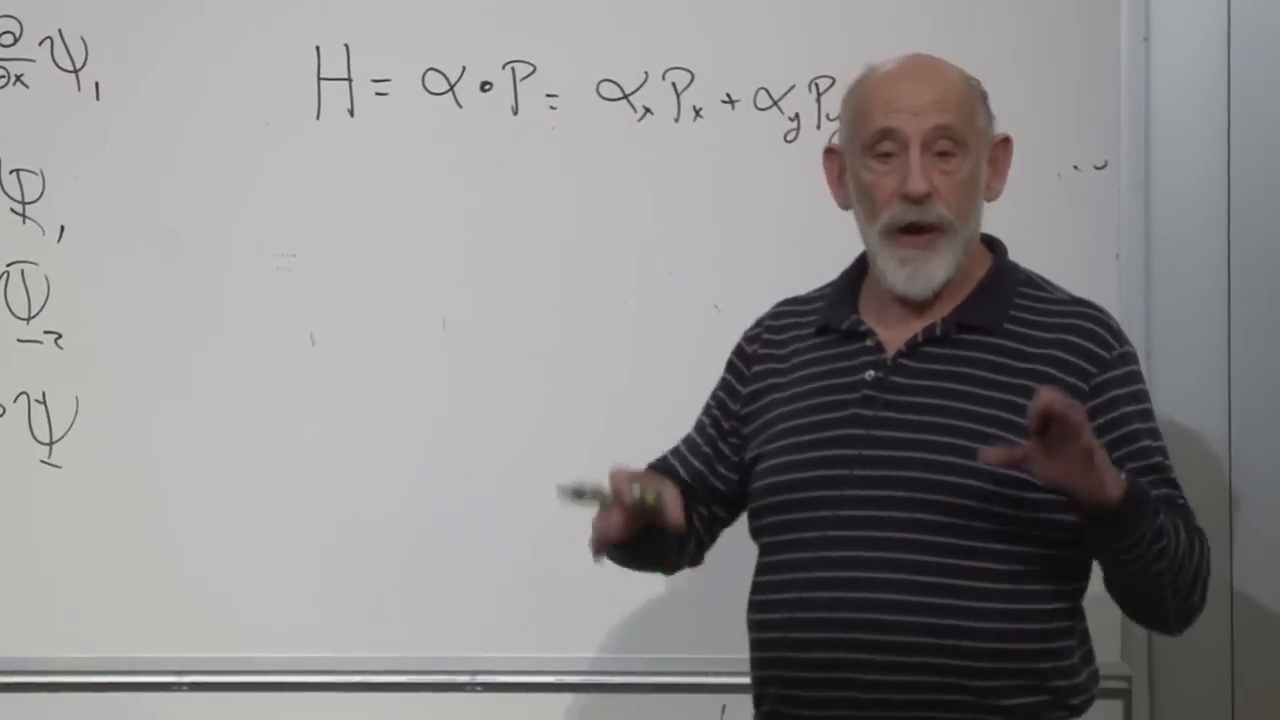
\includegraphics[width=0.94\linewidth]{lecture_10_figure_04.png}
\caption{Dạng giả thiết không khối lượng ba chiều \(H=\boldsymbol{\alpha}\cdot\mathbf P\) tại thời điểm một ma trận được mở rộng thành một vectơ gồm ba ma trận.}
\lectureframe{00:26:00}
\end{figure}

Bắt đầu lại với trường hợp không khối lượng. Ta yêu cầu
\begin{equation}
H^2=\mathbf P^2=P_x^2+P_y^2+P_z^2.
\end{equation}
Khai triển bình phương của Eq.~\eqref{eq:l10-three-d-ansatz},
\begin{align}
H^2
&=\alpha_x^2P_x^2+\alpha_y^2P_y^2\\
&\quad+\alpha_z^2P_z^2\\
&\quad+\{\alpha_x,\alpha_y\}P_xP_y\\
&\quad+\{\alpha_x,\alpha_z\}P_xP_z\\
&\quad+\{\alpha_y,\alpha_z\}P_yP_z.
\end{align}
Các số hạng đường chéo có dạng đúng nếu
\begin{equation}
\alpha_x^2=\alpha_y^2=\alpha_z^2=\mathbb{1},
\end{equation}
và mọi số hạng chéo triệt tiêu nếu
\begin{equation}
\{\alpha_i,\alpha_j\}=0,
\qquad i\ne j.
\label{eq:l10-alpha-anticommutation}
\end{equation}

Ba ma trận \(2\times2\) quen thuộc thực hiện đúng điều này:
\begin{equation}
\sigma_x=
\begin{pmatrix}
0&1\\
1&0
\end{pmatrix},
\quad
\sigma_y=
\begin{pmatrix}
0&-i\\
i&0
\end{pmatrix},
\quad
\sigma_z=
\begin{pmatrix}
1&0\\
0&-1
\end{pmatrix}.
\label{eq:l10-pauli-matrices}
\end{equation}
Vậy một nghiệm là
\begin{equation}
\alpha_i=\sigma_i,
\qquad
H=\boldsymbol{\sigma}\cdot\mathbf P.
\label{eq:l10-weyl-hamiltonian}
\end{equation}

\begin{figure}[htbp]
\centering
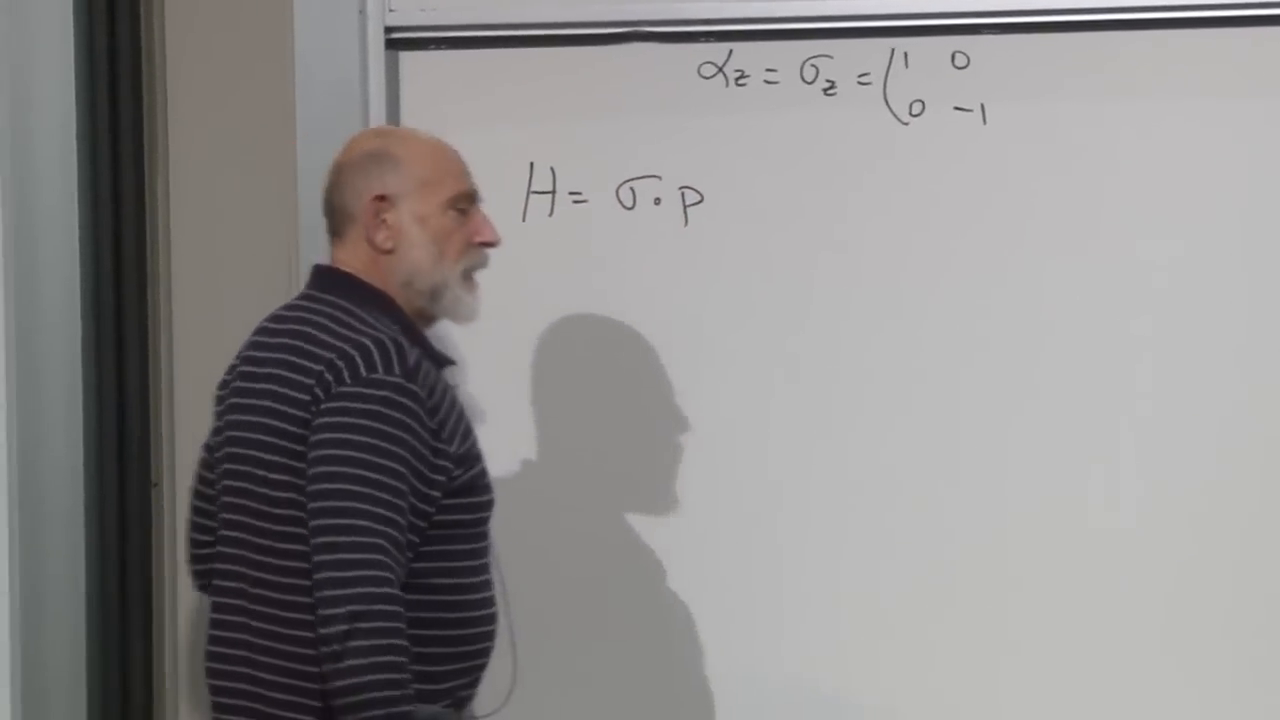
\includegraphics[width=0.94\linewidth]{lecture_10_figure_05.png}
\caption{Hamiltonian không khối lượng dạng gọn \(H=\boldsymbol{\sigma}\cdot\mathbf P\), với \(\alpha_z=\sigma_z\) vẫn được ghi rõ phía trên.}
\lectureframe{00:28:16}
\end{figure}

Với một trạng thái riêng động lượng,
\begin{equation}
\boldsymbol{\sigma}\cdot\mathbf p
=
|\mathbf p|\,\boldsymbol{\sigma}\cdot\widehat{\mathbf p}.
\end{equation}
Toán tử \(\boldsymbol{\sigma}\cdot\widehat{\mathbf p}\) có các trị riêng \(+1\) và \(-1\), nên
\begin{equation}
E=\pm|\mathbf p|.
\end{equation}
Trong lý thuyết hai thành phần này, với năng lượng dương, bậc tự do Pauli định hướng song song với động lượng; với năng lượng âm, nó định hướng ngược chiều. Hướng này bị ràng buộc, chứ không phải là hướng spin có thể điều chỉnh độc lập khi dấu năng lượng đã cố định.

\begin{classroomqa}
\lecturetimestamp{00:30:10}
\audiencequestion{Spin có tự xuất hiện từ phương trình Dirac không, hay được đưa vào vì ta đã biết electron có mômen từ?}
\lecturerresponse{Ở đây, “tự xuất hiện” có nghĩa là “suy ra như một hệ quả”, chứ không phải “biến mất”. Điểm xuất phát là yêu cầu một Hamiltonian tuyến tính theo động lượng, có bình phương bằng \(\mathbf P^2\). Các số thông thường không thể thỏa mãn đại số cần thiết, nhưng ma trận Pauli thì có thể. Vì vậy, cấu trúc hai thành phần của chúng xuất hiện ngay trong quá trình tuyến tính hóa. Điều này không chứng minh rằng hạt nào cũng phải có spin; nó chỉ nói rằng các hạt được mô tả bằng phương trình kiểu Dirac này mang bậc tự do spinor tương ứng.}
\end{classroomqa}

Đây là một trong những bài học cốt lõi của phép dựng này. Các ma trận không phải những nhãn trang trí được thêm vào sau khi tìm ra phương trình tương đối tính. Chính nỗ lực lấy căn bậc hai địa phương của hệ thức tán sắc tương đối tính đã dẫn đến chúng.

\section{Vì sao khối lượng đòi hỏi bốn thành phần}

Hãy thử lặp lại phép dựng khối lượng một chiều mà không mở rộng lý thuyết \(2\times2\):
\begin{equation}
H=\boldsymbol{\sigma}\cdot\mathbf P+\beta m.
\label{eq:l10-failed-mass}
\end{equation}
Giả sử \(\beta^2=\mathbb{1}\). Bình phương chứa các số hạng mong muốn \(\mathbf P^2+m^2\), nhưng còn có cả
\begin{equation}
m\sum_i\{\sigma_i,\beta\}P_i.
\end{equation}
Để loại bỏ số hạng này, một ma trận \(\beta\) phải thỏa mãn
\begin{equation}
\{\sigma_x,\beta\}
=
\{\sigma_y,\beta\}
=
\{\sigma_z,\beta\}
=0.
\label{eq:l10-impossible-beta}
\end{equation}
Không có ma trận \(2\times2\) nào làm được điều đó. Ma trận đơn vị giao hoán với cả ba ma trận Pauli, còn mọi ma trận \(2\times2\) không vết đều là tổ hợp tuyến tính của các ma trận Pauli. Bất kỳ tổ hợp nào như vậy cũng không phản giao hoán với thành phần song song với nó. Đại số \(2\times2\) không có ma trận độc lập thứ tư với tính chất cần thiết.

Giải pháp là mở rộng spinor. Bốn ma trận phản giao hoán đôi một và có bình phương bằng ma trận đơn vị chỉ xuất hiện lần đầu trong một biểu diễn phức \(4\times4\). Không chọn kích thước ma trận này vì không-thời gian có bốn chiều; đây là không gian ma trận nhỏ nhất có thể hiện thực hóa đại số cần thiết.

Có nhiều biểu diễn tương đương. Phép đổi cơ sở đơn nhất của spinor làm thay đổi các phần tử của mọi ma trận mà không làm thay đổi bất kỳ dự đoán vật lý nào. Điều quan trọng là tập hợp các hệ thức trừu tượng
\begin{equation}
\{\alpha_i,\alpha_j\}=2\delta_{ij}\mathbb{1},
\qquad
\{\alpha_i,\beta\}=0,
\qquad
\beta^2=\mathbb{1}.
\label{eq:l10-dirac-algebra}
\end{equation}

\begin{classroomqa}
\lecturetimestamp{00:37:38}
\audiencequestion{Có thể xem \(\beta\) là thành phần thời gian \(\alpha_t\) không?}
\lecturerresponse{Không thể làm vậy một cách trực tiếp. Ba ma trận \(\alpha_i\) không hợp với \(\beta\) thành bốn thành phần của một vectơ Lorentz duy nhất. Thay vào đó, trong ký hiệu hiệp biến, ta định nghĩa \(\beta=\gamma^0\) và \(\alpha_i=\gamma^0\gamma^i\); bốn ma trận \(\gamma^\mu\) thỏa mãn đại số Clifford của không-thời gian.}
\end{classroomqa}

Một biểu diễn khối thuận tiện là
\begin{equation}
\alpha_i=
\begin{pmatrix}
\sigma_i&0\\
0&-\sigma_i
\end{pmatrix},
\qquad
\beta=
\begin{pmatrix}
0&I_2\\
I_2&0
\end{pmatrix}.
\label{eq:l10-block-representation}
\end{equation}
Các ma trận Pauli trong các khối đường chéo bảo đảm các \(\alpha_i\) phản giao hoán đôi một. Các khối đơn vị ngoài đường chéo trong \(\beta\) bảo đảm \(\beta\) phản giao hoán với mọi \(\alpha_i\).

\begin{figure}[htbp]
\centering
\includegraphics[width=0.94\linewidth]{lecture_10_figure_06.png}
\caption{Biểu diễn khối \(4\times4\) trên bảng. Các phương trình phía trên ghi lại các phản giao hoán tử cần có; toàn bộ ma trận được viết thành ký hiệu trong Eq.~\eqref{eq:l10-block-representation}.}
\lectureframe{00:41:10}
\end{figure}

Giờ đây Hamiltonian có khối lượng là
\begin{equation}
H=\boldsymbol{\alpha}\cdot\mathbf P+\beta m
=
\begin{pmatrix}
\boldsymbol{\sigma}\cdot\mathbf P&mI_2\\
mI_2&-\boldsymbol{\sigma}\cdot\mathbf P
\end{pmatrix}.
\label{eq:l10-massive-dirac}
\end{equation}
Dùng Eq.~\eqref{eq:l10-dirac-algebra},
\begin{equation}
H^2=\mathbf P^2+m^2.
\end{equation}
Vì vậy, cấu trúc bốn thành phần không phải phần bổ sung tùy chọn. Đó là cấu trúc nhỏ nhất cho phép đồng thời có động lượng ba chiều và số hạng khối lượng mà vẫn giữ phương trình ở bậc nhất.

\section{Tính chiral và ý nghĩa của các thành phần bổ sung}

Phép mở rộng đã bổ sung khác biệt vật lý nào? Hãy bắt đầu với khối trên không khối lượng,
\begin{equation}
H_R=\boldsymbol{\sigma}\cdot\mathbf P,
\end{equation}
và khối dưới không khối lượng,
\begin{equation}
H_L=-\boldsymbol{\sigma}\cdot\mathbf P.
\end{equation}
Đối với các trạng thái năng lượng dương, spin của khối thứ nhất song song với động lượng, còn spin của khối thứ hai ngược chiều với động lượng. Đó là hai độ xoắn đối nhau. Trong lý thuyết không khối lượng, độ xoắn bất biến dưới các phép biến đổi Lorentz chính tắc, vì không quan sát viên nào có thể vượt một hạt chuyển động như ánh sáng rồi đảo chiều động lượng của nó mà vẫn giữ nguyên spin. Do đó, hai khối mô tả hai khu vực chiral đối nhau.

\begin{classroomqa}
\lecturetimestamp{00:41:28}
\audiencequestion{Trong một chiều, cần thêm một bậc tự do nhị phân để đưa khối lượng vào. Trong ba chiều, khác biệt vật lý tương ứng là gì?}
\lecturerresponse{Đó là tính thuận tay của spinor. Hai khối \(2\times2\) có quan hệ giữa spin và động lượng ngược nhau. Một khối thuận tay phải, khối kia thuận tay trái. Lý thuyết \(4\times4\) chứa cả hai.}
\end{classroomqa}

Số hạng khối lượng trong Eq.~\eqref{eq:l10-massive-dirac} nằm ngoài đường chéo. Nó chuyển biên độ của khối trên sang khối dưới và ngược lại:
\begin{equation}
\beta m
\begin{pmatrix}
\Psi_R\\
\Psi_L
\end{pmatrix}
=
m
\begin{pmatrix}
\Psi_L\\
\Psi_R
\end{pmatrix}.
\end{equation}
Vì vậy, khối lượng là sự ghép nối giữa hai tính chiral đối nhau.

\begin{classroomqa}
\lecturetimestamp{00:43:58}
\audiencequestion{Một hạt không khối lượng có thể đổi tính chiral không?}
\lecturerresponse{Không, với Hamiltonian tự do không khối lượng được trình bày ở đây. Hai khối không ghép với nhau, nên trạng thái ban đầu thuận tay phải hoặc trái sẽ giữ nguyên như vậy. Chính số hạng khối lượng ngoài đường chéo làm trộn chúng khi \(m\ne0\).}
\end{classroomqa}

Cách diễn đạt này chính xác đối với biểu diễn khối, nhưng không nên đẩy quá xa hình ảnh một hạt lật cơ học qua lại giữa hai mũi tên. Phát biểu vật lý ở đây là sự ghép nối ma trận trong phương trình sóng.

\begin{classroomqa}
\lecturetimestamp{00:44:50}
\audiencequestion{Các ma trận này có được hàm chứa trong quaternion không?}
\lecturerresponse{Các ma trận Pauli có liên hệ chặt chẽ với các đơn vị quaternion: bình phương của các ma trận \(-i\sigma_i\) bằng \(-\mathbb{1}\) và phép nhân của chúng tuân theo quy tắc quaternion, tùy theo quy ước định hướng. Các ma trận Dirac đầy đủ đòi hỏi đại số Clifford lớn hơn, và không cần đến mối liên hệ với quaternion cho lập luận tiếp theo.}
\end{classroomqa}

\begin{classroomqa}
\lecturetimestamp{00:46:34}
\audiencequestion{Nếu spin là mômen động lượng, ở đây có số hạng năng lượng riêng nào gắn với nó không?}
\lecturerresponse{Không có số hạng hạt tự do độc lập nào được thêm vào. Cấu trúc spinor đã đi vào Hamiltonian động năng thông qua các ma trận. Ghép spin với một từ trường ngoài sẽ đưa thêm các số hạng tương tác, nhưng đó là một bài toán khác.}
\end{classroomqa}

\section{Các ma trận alpha biểu diễn vận tốc, không phải spin}

Mỗi \(\alpha_i\) có hai trị riêng \(+1\) và hai trị riêng \(-1\). Các thành phần khác nhau không giao hoán, nên không thể đồng thời đo chính xác tất cả chúng. Để xác định một thành phần biểu diễn đại lượng nào, hãy dùng phương trình Heisenberg. Với toán tử \(L\) không phụ thuộc tường minh vào thời gian,
\begin{equation}
\dot L=i[H,L].
\label{eq:l10-heisenberg}
\end{equation}
Quy ước dấu ở đây được xác định theo sự tiến hóa Schr\"odinger \(e^{-iHt}\).

Áp dụng Eq.~\eqref{eq:l10-heisenberg} cho toán tử vị trí \(x\). Các ma trận tác dụng lên các chỉ số spinor và giao hoán với vị trí, trong khi chỉ có \(P_x\) không giao hoán với \(x\):
\begin{align}
\dot x
&=i[\boldsymbol{\alpha}\cdot\mathbf P+\beta m,x]\\
&=i\alpha_x[P_x,x]\\
&=\alpha_x,
\label{eq:l10-velocity}
\end{align}
vì \([P_x,x]=-i\). Do đó, \(\alpha_x\) là thành phần \(x\) của toán tử vận tốc; tương tự,
\begin{equation}
\dot{\mathbf x}=\boldsymbol{\alpha}.
\end{equation}

\begin{classroomqa}
\lecturetimestamp{00:51:50}
\audiencequestion{Phép đo một thành phần vận tốc có thực sự chỉ cho kết quả \(+1\) hoặc \(-1\) không?}
\lecturerresponse{Có, đối với toán tử tức thời \(\alpha_i\) trong đơn vị \(c=1\). Một trạng thái tổng quát không nhất thiết là trạng thái riêng, nên giá trị kỳ vọng của nó có thể nằm ở bất kỳ đâu giữa hai giá trị ấy. Gói sóng được truyền đi một cách liên tục có vận tốc trung bình nhỏ hơn tốc độ ánh sáng khi hạt có khối lượng.}
\end{classroomqa}

Vận tốc không được bảo toàn:
\begin{equation}
\dot\alpha_x=i[H,\alpha_x]\ne0.
\end{equation}
Các số hạng chứa \(\alpha_y\), \(\alpha_z\) và \(\beta\) không giao hoán với \(\alpha_x\). Vì vậy, trạng thái gồm cả thành phần năng lượng dương lẫn âm sẽ biểu hiện một đóng góp dao động nhanh trong vị trí. Hiện tượng này là \emph{chuyển động run}, nghĩa đen là chuyển động rung lắc.

Sau khi lấy trung bình trên khoảng thời gian dài hơn nhiều so với chu kỳ dao động nhanh, vận tốc tương đối tính kỳ vọng là
\begin{equation}
\overline{\mathbf v}=\frac{\mathbf p}{E},
\end{equation}
Với electron chuyển động chậm, biểu thức này rút gọn thành \(\mathbf p/m\).

\begin{classroomqa}
\lecturetimestamp{00:54:40}
\audiencequestion{Electron tự do run mà không chịu lực ngoài thì có vi phạm định luật Newton không?}
\lecturerresponse{Không. Tính bất biến tịnh tiến bảo toàn động lượng, nên \(\dot{\mathbf P}=0\). Toán tử vận tốc Dirac không đơn giản là \(\mathbf P/m\), và thành phần dao động nhanh của nó có thể thay đổi trong khi động lượng vẫn không đổi. Chuyển động lấy trung bình theo thời gian tuân theo hệ thức hạt tự do như dự kiến.}
\end{classroomqa}

\begin{classroomqa}
\lecturetimestamp{00:55:22}
\audiencequestion{Vận tốc có luôn bằng \(c\) không?}
\lecturerresponse{Phép đo tức thời của một \(\alpha_i\) có các trị riêng \(\pm c\), nhưng gói sóng có khối lượng nói chung là một chồng chập và có giá trị kỳ vọng dưới tốc độ ánh sáng. Vận tốc nhóm trung bình của nó là \(\mathbf p/E\).}
\end{classroomqa}

\begin{classroomqa}
\lecturetimestamp{00:55:30}
\audiencequestion{Có thể hình dung dao động này là do khối lượng làm vận tốc biến đổi không?}
\lecturerresponse{Không. Khối lượng là một tham số cố định. Dao động phát sinh từ các toán tử vận tốc và Hamiltonian không giao hoán, hay tương đương từ sự giao thoa giữa các vùng năng lượng, chứ không phải do khối lượng dao động.}
\end{classroomqa}

\begin{classroomqa}
\lecturetimestamp{00:56:22}
\audiencequestion{Phép đo tức thời có thể cho thấy vận tốc hướng theo một chiều, ngay cả khi chuyển động trung bình hướng theo chiều khác không?}
\lecturerresponse{Có. Toán tử thành phần có hai trị riêng xác định, còn các phép đo lặp lại hoặc lấy trung bình theo thời gian cho ta độ trôi liên tục hơn.}
\end{classroomqa}

Cũng cần dùng từ spin một cách cẩn trọng. Các \(\alpha_i\) biến đổi như những thành phần của vận tốc, một vectơ thông thường. Toán tử spin thực sự trong biểu diễn này là
\begin{equation}
\mathbf S=\frac12\boldsymbol{\Sigma},
\qquad
\Sigma_i=
\begin{pmatrix}
\sigma_i&0\\
0&\sigma_i
\end{pmatrix}.
\label{eq:l10-spin-operator}
\end{equation}
Nó khác \(\alpha_i\) ở dấu của khối dưới. Các ma trận có liên hệ chặt chẽ với nhau, nhưng vận tốc và spin không phải cùng một đại lượng quan sát được.

\section{Năng lượng âm và chân không có năng lượng thấp nhất}

Vấn đề năng lượng âm đã xuất hiện ngay cả trước khi có toàn bộ bộ máy ma trận này. Hãy trở lại với sóng truyền sang phải một chiều,
\begin{equation}
H=P.
\end{equation}
Vì \(p\) chạy trên toàn bộ trục số thực nên \(E=p\) không bị chặn dưới.

Chân không không thể chỉ có nghĩa là trạng thái không có hạt. Nó phải là trạng thái mà từ đó không thể lấy thêm năng lượng ra. Nếu trong trạng thái trống, ta có thể thêm một hạt năng lượng âm để hạ năng lượng, rồi thêm hạt khác và cứ tiếp tục vô hạn, thì trạng thái trống ấy không phải là chân không bền vững.

Thống kê Fermi đưa ra một lối thoát mang tính lịch sử. Đặt một electron vào mỗi trạng thái năng lượng âm. Mỗi electron được thêm vào làm giảm tổng năng lượng, nhưng nguyên lý loại trừ chỉ cho phép một electron trong mỗi trạng thái một hạt. Khi mọi trạng thái năng lượng âm đã đầy, không electron nào khác có thể rơi vào vùng ấy. Dirac đồng nhất cấu hình đầy này với chân không.

Cách dựng tương tự sẽ thất bại đối với boson. Một trạng thái có thể chứa số boson tùy ý, nên một mode boson năng lượng âm có thể hấp thụ hạt không giới hạn. Giới hạn fermion \(n=0,1\) được giới thiệu ở đầu bài giảng chính là điều ngăn năng lượng tiếp tục giảm mãi.

\begin{figure}[htbp]
\centering
\includegraphics[width=0.94\linewidth]{lecture_10_figure_07.png}
\caption{Hình ảnh biển Dirac mang tính lịch sử trên bảng: một thang các mức năng lượng âm được lấp đầy tới đường phân chia, bên trên là các trạng thái năng lượng dương.}
\lectureframe{01:02:45}
\end{figure}

\begin{figure}[htbp]
\centering
\begin{adjustbox}{max width=\linewidth}
\begin{tikzpicture}[x=1.05cm,y=0.72cm,>=Latex]
\draw[->] (0,-4.8) -- (0,4.8) node[above] {$E$};
\draw[thick] (-2.9,0) -- (3.2,0) node[right] {$E=0$};
\foreach \y in {-4,-3.3,...,-0.5} {
  \draw (-2.3,\y) -- (2.3,\y);
  \foreach \x in {-1.8,-1.2,...,1.8} {
    \fill[blue!65!black] (\x,\y) circle (1.6pt);
  }
}
\foreach \y in {0.8,1.6,...,4.0} {
  \draw (-2.3,\y) -- (2.3,\y);
}
\draw[red,very thick] (0.6,-2.6) circle (5pt);
\draw[red,->,very thick] (0.6,-2.35) .. controls (1.4,-0.4) and (1.2,1.6) .. (1.5,2.4);
\fill[red] (1.5,2.4) circle (2.5pt);
\node[right,red] at (0.85,-2.6) {hole};
\node[right,red] at (1.7,2.4) {$e^-$};
\node[left] at (-2.5,-2.2) {filled negative-energy states};
\end{tikzpicture}
\end{adjustbox}
\caption{Bản dựng lại rõ ràng về kích thích phía trên biển đầy: đưa một electron năng lượng âm lên cao hơn để lại một lỗ trống năng lượng dương.}
\end{figure}

Hình ảnh biển là cách diễn đạt mang tính lịch sử cho một phép sắp xếp lại toán tử đúng đắn. Không nên nhầm điện tích và năng lượng vô hạn của nó theo nghĩa đen với những đại lượng quan sát được trực tiếp; cách trình bày hiện đại sẽ loại bỏ nhu cầu hình dung electron vật chất lấp đầy không gian.

\section{Lỗ trống là positron}

Khi mọi trạng thái năng lượng âm đều đã bị chiếm, có thể tạo ra hai loại kích thích. Ta có thể thêm một electron năng lượng dương phía trên biển. Hoặc ta có thể lấy đi một electron năng lượng âm và để lại một lỗ trống.

Lỗ trống mang điện tích ngược dấu với electron bị thiếu. Lấy đi điện tích \(-e\) làm điện tích thay đổi một lượng \(+e\). Lỗ trống cũng có năng lượng kích thích dương. Nếu electron bị lấy đi có \(E_-<0\), thì năng lượng đo tương đối với chân không đầy thay đổi một lượng
\begin{equation}
E_{\mathrm{hole}}=-E_->0.
\end{equation}
Lỗ trống là một kích thích có năng lượng dương và điện tích dương: positron.

Một photon có thể kích thích electron trong biển lên một trạng thái năng lượng dương. So với chân không, trạng thái cuối chứa một electron và một positron. Trong giản đồ có thứ tự thời gian, theo quy ước ta vẽ dòng số electron hướng lên đối với electron, còn đường biểu diễn positron có mũi tên ngược chiều. Các mũi tên biểu thị dòng số fermion hoặc dòng điện tích; chúng không phải những vectơ vận tốc cổ điển nhỏ bé.

\begin{classroomqa}
\lecturetimestamp{01:05:14}
\audiencequestion{Hình ảnh này có đòi hỏi số electron và positron bằng nhau không?}
\lecturerresponse{Không phải trong một trạng thái bất kỳ. Bắt đầu từ chân không và tạo một cặp trung hòa thì có một hạt mỗi loại, nhưng một trạng thái có thể vốn đã chứa số electron dư hoặc số positron dư. Bảo toàn điện tích ràng buộc các phản ứng; nó không đòi hỏi mọi trạng thái khả dĩ phải có số lượng hai loại hạt bằng nhau.}
\end{classroomqa}

Ban đầu Dirac chưa biết rằng lỗ trống sẽ là một hạt có khối lượng bằng khối lượng electron và chỉ khác về điện tích cùng các số lượng tử cộng tính khác. Phương trình và phép dựng lỗ trống đã dẫn đến dự đoán ấy trước khi positron được đưa vào danh mục hạt quen thuộc.

\section{Một trường fermion chứa cả electron lẫn positron}

Toán tử trường đưa hình ảnh mang tính lịch sử này vào đại số hiện đại. Tạm thời bỏ qua các chỉ số spinor, hệ số chuẩn hóa và sự phụ thuộc thời gian. Một trường một chiều có thể được khai triển dưới dạng sơ đồ như sau:
\begin{equation}
\psi(x)
\sim
\int_{-\infty}^{\infty}dp\,a(p)e^{ipx}.
\label{eq:l10-full-field-integral}
\end{equation}
Với hệ thức tán sắc của sóng truyền sang phải \(E=p\), \(p\) dương ứng với năng lượng dương, còn \(p\) âm ứng với năng lượng âm. Tách tích phân:
\begin{equation}
\psi(x)
\sim
\int_0^\infty dp\,a(p)e^{ipx}
+
\int_{-\infty}^0 dp\,a(p)e^{ipx}.
\end{equation}
Trong số hạng thứ hai, đặt \(p=-q\), với \(q>0\), rồi diễn giải lại phép hủy electron năng lượng âm trong trạng thái đầy thành phép tạo positron:
\begin{equation}
b^\dagger(q):=a(-q).
\end{equation}
Khi đó
\begin{equation}
\psi(x)
\sim
\int_0^\infty dp\,
\left[
a(p)e^{ipx}
+
b^\dagger(p)e^{-ipx}
\right].
\label{eq:l10-electron-positron-split}
\end{equation}
Dấu chính xác của các pha sóng phẳng phụ thuộc vào quy ước không-thời gian; nội dung bất biến là \(\psi\) chứa một toán tử hủy electron và một toán tử tạo positron.

\begin{figure}[htbp]
\centering
\includegraphics[width=0.94\linewidth]{lecture_10_figure_08.png}
\caption{Tích phân trường được tách thành các vùng năng lượng dương và âm. Dòng dưới đổi nhãn toán tử electron năng lượng âm thành toán tử tạo positron.}
\lectureframe{01:11:35}
\end{figure}

Đây là lúc sự đối xứng giữa trạng thái đầy và trống trong Eq.~\eqref{eq:l10-fermion-mode} phát huy tác dụng. Đối với fermion, đại số toán tử cho phép đổi nhãn như vậy mà không làm thay đổi cấu trúc phản giao hoán.

Một tương tác điện từ dạng sơ đồ có dạng
\begin{equation}
H_{\mathrm{int}}
\sim
\int dx\,\psi^\dagger(x)\psi(x)A(x),
\label{eq:l10-qed-schematic}
\end{equation}
trong đó \(A\) ký hiệu trường photon. Vì mỗi trường fermion đều chứa các thành phần electron và positron, một toán tử địa phương duy nhất chứa một số kênh:
\begin{align}
e^-&\longrightarrow e^-+\gamma,\\
e^-+e^+&\longrightarrow\gamma,\\
\gamma&\longrightarrow e^-+e^+,
\end{align}
cùng với các quá trình ngược và quá trình bắt chéo tương ứng. Bảo toàn năng lượng-động lượng quyết định kênh nào có thể xảy ra về mặt động học trong một môi trường cụ thể. Chẳng hạn, một photon thực cô lập trong chân không không thể tạo ra một cặp nếu không có hạt khác nhận động lượng giật lùi, dù đỉnh tương tác địa phương vẫn hiện diện.

\begin{figure}[htbp]
\centering
\includegraphics[width=0.94\linewidth]{lecture_10_figure_09.png}
\caption{Bảng đặt cạnh nhau quá trình phát xạ electron, hủy cặp và tương tác dạng sơ đồ \(\psi^\dagger\psi A\). Các lựa chọn khác nhau từ cùng những toán tử trường tạo ra các kênh khác nhau.}
\lectureframe{01:13:30}
\end{figure}

Vì vậy, một tích trường gọn duy nhất tổ chức được nhiều phản ứng thoạt nhìn có vẻ khác nhau. Về sau, Feynman đã đưa ra các quy tắc giản đồ có hệ thống để tính biên độ, nhưng phần lớn cấu trúc toán tử đã hiện rõ ở đây.

\section{Cách diễn đạt chân không hiện đại và phép tương tự biển Fermi}

\begin{classroomqa}
\lecturetimestamp{01:14:20}
\audiencequestion{Các nhà vật lý hiện đại mô tả điều này thế nào mà không xem chân không là một biển Dirac theo nghĩa đen?}
\lecturerresponse{Họ thực hiện trực tiếp phép diễn giải lại toán tử. Phép hủy electron năng lượng âm được đổi tên thành phép tạo positron năng lượng dương, còn chân không được định nghĩa là trạng thái bị mọi toán tử hủy electron và positron triệt tiêu. Cách trình bày thu được đối xứng giữa hạt và phản hạt, không cần đến một biển vật chất.}
\end{classroomqa}

Biển Dirac trong lịch sử vẫn hữu ích vì logic của nó có một phép tương tự cô đọng trong vật chất ngưng tụ. Trong tinh thể, một số electron cố định lấp đầy các trạng thái một hạt có năng lượng thấp nhất cho đến mức Fermi. Trạng thái cơ bản đã lấp đầy không phải là trống rỗng. Khi đưa một electron lên trên mức đó, một trạng thái bên dưới mức ấy bị bỏ trống. So với nền đã lấp đầy, lỗ trống mang năng lượng kích thích dương và có thể hoạt động như một hạt tải điện dương.

Có những khác biệt quan trọng. Lỗ trống trong chất rắn tồn tại trong một môi trường, còn khối lượng hiệu dụng và đáp ứng điện tích của nó phụ thuộc vào cấu trúc vùng năng lượng. Positron là một phản hạt sơ cấp trong trường lượng tử tương đối tính. Dù vậy, đại số hạt-lỗ trống chung khiến phép tương tự này rất hữu ích.

\begin{classroomqa}
\lecturetimestamp{01:17:14}
\audiencequestion{Lý thuyết Klein--Gordon cho boson có gặp phải sự sụp đổ dây chuyền xuống các trạng thái năng lượng âm tương tự không?}
\lecturerresponse{Không. Trường Klein--Gordon phức được lượng tử hóa đúng cách được mô tả bằng các hạt và phản hạt có năng lượng dương, không cần lấp đầy một biển boson. Phương trình bậc hai và cấu trúc chính tắc của nó khác với cách xây dựng Hamiltonian Dirac, vì vậy lập luận lịch sử về biển fermion không thể áp dụng nguyên vẹn ở đây.}
\end{classroomqa}

\begin{classroomqa}
\lecturetimestamp{01:17:30}
\audiencequestion{Spin một của boson bắt nguồn từ đâu?}
\lecturerresponse{Không bắt nguồn từ phép tuyến tính hóa bằng ma trận Pauli được dùng ở đây. Trường spin một có quy luật biến đổi Lorentz và phương trình trường riêng. Phép suy dẫn hiện tại giải thích cấu trúc spinor của fermion Dirac, chứ không phải mọi spin hạt có thể có.}
\end{classroomqa}

\begin{classroomqa}
\lecturetimestamp{01:17:46}
\audiencequestion{Vì sao thống kê Fermi là thiết yếu đối với nghiệm năng lượng âm?}
\lecturerresponse{Vì nguyên lý loại trừ giới hạn mỗi trạng thái chỉ chứa một electron. Khi mọi trạng thái năng lượng âm đã có electron chiếm giữ, không electron nào có thể rơi thêm vào đó. Số hạt boson chiếm giữ không có giới hạn như vậy, nên một biển boson năng lượng âm theo nghĩa đen vẫn không có đáy.}
\end{classroomqa}

\begin{classroomqa}
\lecturetimestamp{01:20:02}
\audiencequestion{Electron và positron có đơn giản là một bậc tự do nhị phân khác, giống như điện tích không?}
\lecturerresponse{Xét về phép đếm trạng thái, trường Dirac có khối lượng có hai trạng thái spin electron và hai trạng thái spin positron, nên hai nhãn nhị phân là một cách ghi nhớ hữu ích. Nhưng hạt và phản hạt không phải là một qubit nội tại có thể quay độc lập của một electron: mọi electron đều có điện tích \(-e\), mọi positron đều có điện tích \(+e\), và sự phân biệt này xuất hiện từ các sector tần số dương và âm sau khi lượng tử hóa.}
\end{classroomqa}

Biển vô hạn đặt ra câu hỏi cuối cùng.

\begin{classroomqa}
\lecturetimestamp{01:20:54}
\audiencequestion{Biển Dirac vô hạn có tạo ra hằng số vũ trụ vô hạn không?}
\lecturerresponse{Điều này làm lộ rõ vấn đề năng lượng chân không. Các mode năng lượng điểm không của boson đóng góp \(+\tfrac12\hbar\omega\), còn các mode fermion đóng góp với dấu ngược lại. Có thể xảy ra những sự triệt tiêu hình thức nếu các phổ khớp nhau, nhưng phổ electron và photon không khớp nhau, nên dự kiến sẽ còn lại một phần dư khổng lồ. Khi không có hấp dẫn, có thể trừ đi một hằng số khỏi Hamiltonian vì chỉ các hiệu năng lượng mới có ý nghĩa. Khi có hấp dẫn, năng lượng chân không tuyệt đối cũng gây hấp dẫn, nên phép trừ trở thành một vấn đề vật lý chứ không còn chỉ là thao tác ghi sổ.}
\end{classroomqa}

Lần trở lại cuối cùng là với ý nghĩa của khối lượng.

\begin{classroomqa}
\lecturetimestamp{01:22:56}
\audiencequestion{Ta có thể nói thêm điều gì về mối liên hệ giữa khối lượng với các thành phần tay trái và tay phải?}
\lecturerresponse{Phát biểu chính xác đã có trong Hamiltonian: số hạng ngoài đường chéo \(m\beta\) thực hiện phép biến đổi từ khối chiral này sang khối kia. Mọi hình dung cơ học hơn về sự lật vi mô chỉ là tùy chọn và không tránh khỏi thiếu đầy đủ.}
\end{classroomqa}
\end{document}